\documentclass[twoside]{book}

% Packages required by doxygen
\usepackage{fixltx2e}
\usepackage{calc}
\usepackage{doxygen}
\usepackage[export]{adjustbox} % also loads graphicx
\usepackage{graphicx}
\usepackage[utf8]{inputenc}
\usepackage{makeidx}
\usepackage{multicol}
\usepackage{multirow}
\PassOptionsToPackage{warn}{textcomp}
\usepackage{textcomp}
\usepackage[nointegrals]{wasysym}
\usepackage[table]{xcolor}

% Font selection
\usepackage[T1]{fontenc}
\usepackage[scaled=.90]{helvet}
\usepackage{courier}
\usepackage{amssymb}
\usepackage{sectsty}
\renewcommand{\familydefault}{\sfdefault}
\allsectionsfont{%
  \fontseries{bc}\selectfont%
  \color{darkgray}%
}
\renewcommand{\DoxyLabelFont}{%
  \fontseries{bc}\selectfont%
  \color{darkgray}%
}
\newcommand{\+}{\discretionary{\mbox{\scriptsize$\hookleftarrow$}}{}{}}

% Page & text layout
\usepackage{geometry}
\geometry{%
  a4paper,%
  top=2.5cm,%
  bottom=2.5cm,%
  left=2.5cm,%
  right=2.5cm%
}
\tolerance=750
\hfuzz=15pt
\hbadness=750
\setlength{\emergencystretch}{15pt}
\setlength{\parindent}{0cm}
\setlength{\parskip}{3ex plus 2ex minus 2ex}
\makeatletter
\renewcommand{\paragraph}{%
  \@startsection{paragraph}{4}{0ex}{-1.0ex}{1.0ex}{%
    \normalfont\normalsize\bfseries\SS@parafont%
  }%
}
\renewcommand{\subparagraph}{%
  \@startsection{subparagraph}{5}{0ex}{-1.0ex}{1.0ex}{%
    \normalfont\normalsize\bfseries\SS@subparafont%
  }%
}
\makeatother

% Headers & footers
\usepackage{fancyhdr}
\pagestyle{fancyplain}
\fancyhead[LE]{\fancyplain{}{\bfseries\thepage}}
\fancyhead[CE]{\fancyplain{}{}}
\fancyhead[RE]{\fancyplain{}{\bfseries\leftmark}}
\fancyhead[LO]{\fancyplain{}{\bfseries\rightmark}}
\fancyhead[CO]{\fancyplain{}{}}
\fancyhead[RO]{\fancyplain{}{\bfseries\thepage}}
\fancyfoot[LE]{\fancyplain{}{}}
\fancyfoot[CE]{\fancyplain{}{}}
\fancyfoot[RE]{\fancyplain{}{\bfseries\scriptsize Generated by Doxygen }}
\fancyfoot[LO]{\fancyplain{}{\bfseries\scriptsize Generated by Doxygen }}
\fancyfoot[CO]{\fancyplain{}{}}
\fancyfoot[RO]{\fancyplain{}{}}
\renewcommand{\footrulewidth}{0.4pt}
\renewcommand{\chaptermark}[1]{%
  \markboth{#1}{}%
}
\renewcommand{\sectionmark}[1]{%
  \markright{\thesection\ #1}%
}

% Indices & bibliography
\usepackage{natbib}
\usepackage[titles]{tocloft}
\setcounter{tocdepth}{3}
\setcounter{secnumdepth}{5}
\makeindex

% Custom commands
\newcommand{\clearemptydoublepage}{%
  \newpage{\pagestyle{empty}\cleardoublepage}%
}

\usepackage{caption}
\captionsetup{labelsep=space,justification=centering,font={bf},singlelinecheck=off,skip=4pt,position=top}

%===== C O N T E N T S =====

\begin{document}

% Titlepage & ToC
\pagenumbering{alph}
\begin{titlepage}
\vspace*{7cm}
\begin{center}%
{\Large Enocean \\[1ex]\large 1.\+0 }\\
\vspace*{1cm}
{\large Generated by Doxygen 1.8.12}\\
\end{center}
\end{titlepage}
\clearemptydoublepage
\pagenumbering{roman}
\tableofcontents
\clearemptydoublepage
\pagenumbering{arabic}

%--- Begin generated contents ---
\chapter{Namespace Index}
\section{Packages}
Here are the packages with brief descriptions (if available)\+:\begin{DoxyCompactList}
\item\contentsline{section}{{\bf ch} }{\pageref{namespacech}}{}
\item\contentsline{section}{{\bf ch.\+bfh} }{\pageref{namespacech_1_1bfh}}{}
\item\contentsline{section}{{\bf ch.\+bfh.\+gr33nopo55um} }{\pageref{namespacech_1_1bfh_1_1gr33nopo55um}}{}
\item\contentsline{section}{{\bf ch.\+bfh.\+gr33nopo55um.\+enocean} }{\pageref{namespacech_1_1bfh_1_1gr33nopo55um_1_1enocean}}{}
\item\contentsline{section}{{\bf ch.\+bfh.\+gr33nopo55um.\+enocean.\+application} }{\pageref{namespacech_1_1bfh_1_1gr33nopo55um_1_1enocean_1_1application}}{}
\item\contentsline{section}{{\bf ch.\+bfh.\+gr33nopo55um.\+enocean.\+helper} }{\pageref{namespacech_1_1bfh_1_1gr33nopo55um_1_1enocean_1_1helper}}{}
\item\contentsline{section}{{\bf ch.\+bfh.\+gr33nopo55um.\+enocean.\+persistence} }{\pageref{namespacech_1_1bfh_1_1gr33nopo55um_1_1enocean_1_1persistence}}{}
\item\contentsline{section}{{\bf ch.\+bfh.\+gr33nopo55um.\+enocean.\+telegram} }{\pageref{namespacech_1_1bfh_1_1gr33nopo55um_1_1enocean_1_1telegram}}{}
\item\contentsline{section}{{\bf ch.\+bfh.\+gr33nopo55um.\+enocean.\+test} }{\pageref{namespacech_1_1bfh_1_1gr33nopo55um_1_1enocean_1_1test}}{}
\end{DoxyCompactList}

\chapter{Hierarchical Index}
\section{Class Hierarchy}
This inheritance list is sorted roughly, but not completely, alphabetically\+:\begin{DoxyCompactList}
\item \contentsline{section}{All}{\pageref{classAll}}{}
\item \contentsline{section}{An}{\pageref{classAn}}{}
\item \contentsline{section}{Application}{\pageref{classch_1_1bfh_1_1gr33nopo55um_1_1enocean_1_1application_1_1Application}}{}
\item \contentsline{section}{Checksum}{\pageref{classChecksum}}{}
\item \contentsline{section}{Class}{\pageref{classClass}}{}
\item \contentsline{section}{Class}{\pageref{classClass}}{}
\item \contentsline{section}{C\+RC}{\pageref{classch_1_1bfh_1_1gr33nopo55um_1_1enocean_1_1helper_1_1CRC}}{}
\item \contentsline{section}{DB}{\pageref{classDB}}{}
\item \contentsline{section}{diagnosis}{\pageref{classdiagnosis}}{}
\item \contentsline{section}{Encode\+Decode}{\pageref{interfacech_1_1bfh_1_1gr33nopo55um_1_1enocean_1_1telegram_1_1EncodeDecode}}{}
\begin{DoxyCompactList}
\item \contentsline{section}{Telegram\+Header}{\pageref{classch_1_1bfh_1_1gr33nopo55um_1_1enocean_1_1telegram_1_1TelegramHeader}}{}
\begin{DoxyCompactList}
\item \contentsline{section}{Common\+Command}{\pageref{classch_1_1bfh_1_1gr33nopo55um_1_1enocean_1_1telegram_1_1CommonCommand}}{}
\item \contentsline{section}{Dummy}{\pageref{classch_1_1bfh_1_1gr33nopo55um_1_1enocean_1_1telegram_1_1Dummy}}{}
\item \contentsline{section}{Event}{\pageref{classch_1_1bfh_1_1gr33nopo55um_1_1enocean_1_1telegram_1_1Event}}{}
\item \contentsline{section}{Radio802}{\pageref{classch_1_1bfh_1_1gr33nopo55um_1_1enocean_1_1telegram_1_1Radio802}}{}
\item \contentsline{section}{Radio\+E\+R\+P1}{\pageref{classch_1_1bfh_1_1gr33nopo55um_1_1enocean_1_1telegram_1_1RadioERP1}}{}
\item \contentsline{section}{Radio\+E\+R\+P2}{\pageref{classch_1_1bfh_1_1gr33nopo55um_1_1enocean_1_1telegram_1_1RadioERP2}}{}
\item \contentsline{section}{Radio\+Message}{\pageref{classch_1_1bfh_1_1gr33nopo55um_1_1enocean_1_1telegram_1_1RadioMessage}}{}
\item \contentsline{section}{Radio\+Sub\+Tel}{\pageref{classch_1_1bfh_1_1gr33nopo55um_1_1enocean_1_1telegram_1_1RadioSubTel}}{}
\item \contentsline{section}{Remote\+Man\+Command}{\pageref{classch_1_1bfh_1_1gr33nopo55um_1_1enocean_1_1telegram_1_1RemoteManCommand}}{}
\item \contentsline{section}{Response}{\pageref{classch_1_1bfh_1_1gr33nopo55um_1_1enocean_1_1telegram_1_1Response}}{}
\item \contentsline{section}{Smart\+Ack\+Command}{\pageref{classch_1_1bfh_1_1gr33nopo55um_1_1enocean_1_1telegram_1_1SmartAckCommand}}{}
\end{DoxyCompactList}
\end{DoxyCompactList}
\item \contentsline{section}{Enocea\+Listener}{\pageref{classch_1_1bfh_1_1gr33nopo55um_1_1enocean_1_1application_1_1EnoceaListener}}{}
\item \contentsline{section}{E\+R\+P1}{\pageref{classERP1}}{}
\item \contentsline{section}{E\+R\+P2}{\pageref{classERP2}}{}
\item \contentsline{section}{Logic}{\pageref{classLogic}}{}
\item \contentsline{section}{Main}{\pageref{classMain}}{}
\item \contentsline{section}{Physical}{\pageref{classPhysical}}{}
\item \contentsline{section}{Radio}{\pageref{classRadio}}{}
\item \contentsline{section}{Read\+Config}{\pageref{classch_1_1bfh_1_1gr33nopo55um_1_1enocean_1_1helper_1_1ReadConfig}}{}
\item \contentsline{section}{remote}{\pageref{classremote}}{}
\item \contentsline{section}{Seed\+DB}{\pageref{classch_1_1bfh_1_1gr33nopo55um_1_1enocean_1_1persistence_1_1SeedDB}}{}
\item \contentsline{section}{Sender}{\pageref{classch_1_1bfh_1_1gr33nopo55um_1_1enocean_1_1test_1_1Sender}}{}
\item \contentsline{section}{Serveral}{\pageref{classServeral}}{}
\item \contentsline{section}{S\+M\+A\+R\+T\+\_\+\+A\+C\+K\+\_\+\+C\+O\+M\+M\+A\+ND}{\pageref{classSMART__ACK__COMMAND}}{}
\item \contentsline{section}{Store}{\pageref{classch_1_1bfh_1_1gr33nopo55um_1_1enocean_1_1persistence_1_1Store}}{}
\item \contentsline{section}{Telegram\+D\+B\+Factory}{\pageref{classch_1_1bfh_1_1gr33nopo55um_1_1enocean_1_1persistence_1_1TelegramDBFactory}}{}
\item \contentsline{section}{Tester}{\pageref{classch_1_1bfh_1_1gr33nopo55um_1_1enocean_1_1test_1_1Tester}}{}
\item \contentsline{section}{This}{\pageref{classThis}}{}
\item \contentsline{section}{Time}{\pageref{classTime}}{}
\item \contentsline{section}{Time\+Logger}{\pageref{classch_1_1bfh_1_1gr33nopo55um_1_1enocean_1_1helper_1_1TimeLogger}}{}
\item \contentsline{section}{Used}{\pageref{classUsed}}{}
\item \contentsline{section}{When}{\pageref{classWhen}}{}
\end{DoxyCompactList}

\chapter{Class Index}
\section{Class List}
Here are the classes, structs, unions and interfaces with brief descriptions\+:\begin{DoxyCompactList}
\item\contentsline{section}{{\bf All} }{\pageref{classAll}}{}
\item\contentsline{section}{{\bf An} }{\pageref{classAn}}{}
\item\contentsline{section}{{\bf Application} }{\pageref{classch_1_1bfh_1_1gr33nopo55um_1_1enocean_1_1application_1_1Application}}{}
\item\contentsline{section}{{\bf Checksum} }{\pageref{classChecksum}}{}
\item\contentsline{section}{{\bf Class} }{\pageref{classClass}}{}
\item\contentsline{section}{{\bf Class} }{\pageref{classClass}}{}
\item\contentsline{section}{{\bf Common\+Command} }{\pageref{classch_1_1bfh_1_1gr33nopo55um_1_1enocean_1_1telegram_1_1CommonCommand}}{}
\item\contentsline{section}{{\bf C\+RC} }{\pageref{classch_1_1bfh_1_1gr33nopo55um_1_1enocean_1_1helper_1_1CRC}}{}
\item\contentsline{section}{{\bf DB} }{\pageref{classDB}}{}
\item\contentsline{section}{{\bf diagnosis} }{\pageref{classdiagnosis}}{}
\item\contentsline{section}{{\bf Dummy} }{\pageref{classch_1_1bfh_1_1gr33nopo55um_1_1enocean_1_1telegram_1_1Dummy}}{}
\item\contentsline{section}{{\bf Encode\+Decode} }{\pageref{interfacech_1_1bfh_1_1gr33nopo55um_1_1enocean_1_1telegram_1_1EncodeDecode}}{}
\item\contentsline{section}{{\bf Enocea\+Listener} }{\pageref{classch_1_1bfh_1_1gr33nopo55um_1_1enocean_1_1application_1_1EnoceaListener}}{}
\item\contentsline{section}{{\bf E\+R\+P1} }{\pageref{classERP1}}{}
\item\contentsline{section}{{\bf E\+R\+P2} }{\pageref{classERP2}}{}
\item\contentsline{section}{{\bf Event} }{\pageref{classch_1_1bfh_1_1gr33nopo55um_1_1enocean_1_1telegram_1_1Event}}{}
\item\contentsline{section}{{\bf Logic} }{\pageref{classLogic}}{}
\item\contentsline{section}{{\bf Main} }{\pageref{classMain}}{}
\item\contentsline{section}{{\bf Physical} }{\pageref{classPhysical}}{}
\item\contentsline{section}{{\bf Radio} }{\pageref{classRadio}}{}
\item\contentsline{section}{{\bf Radio802} }{\pageref{classch_1_1bfh_1_1gr33nopo55um_1_1enocean_1_1telegram_1_1Radio802}}{}
\item\contentsline{section}{{\bf Radio\+E\+R\+P1} }{\pageref{classch_1_1bfh_1_1gr33nopo55um_1_1enocean_1_1telegram_1_1RadioERP1}}{}
\item\contentsline{section}{{\bf Radio\+E\+R\+P2} }{\pageref{classch_1_1bfh_1_1gr33nopo55um_1_1enocean_1_1telegram_1_1RadioERP2}}{}
\item\contentsline{section}{{\bf Radio\+Message} }{\pageref{classch_1_1bfh_1_1gr33nopo55um_1_1enocean_1_1telegram_1_1RadioMessage}}{}
\item\contentsline{section}{{\bf Radio\+Sub\+Tel} }{\pageref{classch_1_1bfh_1_1gr33nopo55um_1_1enocean_1_1telegram_1_1RadioSubTel}}{}
\item\contentsline{section}{{\bf Read\+Config} }{\pageref{classch_1_1bfh_1_1gr33nopo55um_1_1enocean_1_1helper_1_1ReadConfig}}{}
\item\contentsline{section}{{\bf remote} }{\pageref{classremote}}{}
\item\contentsline{section}{{\bf Remote\+Man\+Command} }{\pageref{classch_1_1bfh_1_1gr33nopo55um_1_1enocean_1_1telegram_1_1RemoteManCommand}}{}
\item\contentsline{section}{{\bf Response} }{\pageref{classch_1_1bfh_1_1gr33nopo55um_1_1enocean_1_1telegram_1_1Response}}{}
\item\contentsline{section}{{\bf Seed\+DB} }{\pageref{classch_1_1bfh_1_1gr33nopo55um_1_1enocean_1_1persistence_1_1SeedDB}}{}
\item\contentsline{section}{{\bf Sender} }{\pageref{classch_1_1bfh_1_1gr33nopo55um_1_1enocean_1_1test_1_1Sender}}{}
\item\contentsline{section}{{\bf Serveral} }{\pageref{classServeral}}{}
\item\contentsline{section}{{\bf S\+M\+A\+R\+T\+\_\+\+A\+C\+K\+\_\+\+C\+O\+M\+M\+A\+ND} }{\pageref{classSMART__ACK__COMMAND}}{}
\item\contentsline{section}{{\bf Smart\+Ack\+Command} }{\pageref{classch_1_1bfh_1_1gr33nopo55um_1_1enocean_1_1telegram_1_1SmartAckCommand}}{}
\item\contentsline{section}{{\bf Store} }{\pageref{classch_1_1bfh_1_1gr33nopo55um_1_1enocean_1_1persistence_1_1Store}}{}
\item\contentsline{section}{{\bf Telegram\+D\+B\+Factory} }{\pageref{classch_1_1bfh_1_1gr33nopo55um_1_1enocean_1_1persistence_1_1TelegramDBFactory}}{}
\item\contentsline{section}{{\bf Telegram\+Header} }{\pageref{classch_1_1bfh_1_1gr33nopo55um_1_1enocean_1_1telegram_1_1TelegramHeader}}{}
\item\contentsline{section}{{\bf Tester} }{\pageref{classch_1_1bfh_1_1gr33nopo55um_1_1enocean_1_1test_1_1Tester}}{}
\item\contentsline{section}{{\bf This} }{\pageref{classThis}}{}
\item\contentsline{section}{{\bf Time} }{\pageref{classTime}}{}
\item\contentsline{section}{{\bf Time\+Logger} }{\pageref{classch_1_1bfh_1_1gr33nopo55um_1_1enocean_1_1helper_1_1TimeLogger}}{}
\item\contentsline{section}{{\bf Used} }{\pageref{classUsed}}{}
\item\contentsline{section}{{\bf When} }{\pageref{classWhen}}{}
\end{DoxyCompactList}

\chapter{File Index}
\section{File List}
Here is a list of all files with brief descriptions\+:\begin{DoxyCompactList}
\item\contentsline{section}{src/ch/bfh/gr33nopo55um/enocean/application/\hyperlink{_application_8java}{Application.\+java} }{\pageref{_application_8java}}{}
\item\contentsline{section}{src/ch/bfh/gr33nopo55um/enocean/application/\hyperlink{_enocea_listener_8java}{Enocea\+Listener.\+java} }{\pageref{_enocea_listener_8java}}{}
\item\contentsline{section}{src/ch/bfh/gr33nopo55um/enocean/helper/\hyperlink{_c_r_c_8java}{C\+R\+C.\+java} }{\pageref{_c_r_c_8java}}{}
\item\contentsline{section}{src/ch/bfh/gr33nopo55um/enocean/helper/\hyperlink{_read_config_8java}{Read\+Config.\+java} }{\pageref{_read_config_8java}}{}
\item\contentsline{section}{src/ch/bfh/gr33nopo55um/enocean/helper/\hyperlink{_seed_d_b_8java}{Seed\+D\+B.\+java} }{\pageref{_seed_d_b_8java}}{}
\item\contentsline{section}{src/ch/bfh/gr33nopo55um/enocean/helper/\hyperlink{_telegram_d_b_factory_8java}{Telegram\+D\+B\+Factory.\+java} }{\pageref{_telegram_d_b_factory_8java}}{}
\item\contentsline{section}{src/ch/bfh/gr33nopo55um/enocean/persistence/\hyperlink{_store_8java}{Store.\+java} }{\pageref{_store_8java}}{}
\item\contentsline{section}{src/ch/bfh/gr33nopo55um/enocean/telegram/\hyperlink{_common_command_8java}{Common\+Command.\+java} }{\pageref{_common_command_8java}}{}
\item\contentsline{section}{src/ch/bfh/gr33nopo55um/enocean/telegram/\hyperlink{_dumy_8java}{Dumy.\+java} }{\pageref{_dumy_8java}}{}
\item\contentsline{section}{src/ch/bfh/gr33nopo55um/enocean/telegram/\hyperlink{_encode_decode_8java}{Encode\+Decode.\+java} }{\pageref{_encode_decode_8java}}{}
\item\contentsline{section}{src/ch/bfh/gr33nopo55um/enocean/telegram/\hyperlink{ch_2bfh_2gr33nopo55um_2enocean_2telegram_2_event_8java}{Event.\+java} }{\pageref{ch_2bfh_2gr33nopo55um_2enocean_2telegram_2_event_8java}}{}
\item\contentsline{section}{src/ch/bfh/gr33nopo55um/enocean/telegram/\hyperlink{_radio802_8java}{Radio802.\+java} }{\pageref{_radio802_8java}}{}
\item\contentsline{section}{src/ch/bfh/gr33nopo55um/enocean/telegram/\hyperlink{_radio_e_r_p1_8java}{Radio\+E\+R\+P1.\+java} }{\pageref{_radio_e_r_p1_8java}}{}
\item\contentsline{section}{src/ch/bfh/gr33nopo55um/enocean/telegram/\hyperlink{_radio_e_r_p2_8java}{Radio\+E\+R\+P2.\+java} }{\pageref{_radio_e_r_p2_8java}}{}
\item\contentsline{section}{src/ch/bfh/gr33nopo55um/enocean/telegram/\hyperlink{ch_2bfh_2gr33nopo55um_2enocean_2telegram_2_radio_message_8java}{Radio\+Message.\+java} }{\pageref{ch_2bfh_2gr33nopo55um_2enocean_2telegram_2_radio_message_8java}}{}
\item\contentsline{section}{src/ch/bfh/gr33nopo55um/enocean/telegram/\hyperlink{ch_2bfh_2gr33nopo55um_2enocean_2telegram_2_radio_sub_tel_8java}{Radio\+Sub\+Tel.\+java} }{\pageref{ch_2bfh_2gr33nopo55um_2enocean_2telegram_2_radio_sub_tel_8java}}{}
\item\contentsline{section}{src/ch/bfh/gr33nopo55um/enocean/telegram/\hyperlink{ch_2bfh_2gr33nopo55um_2enocean_2telegram_2_remote_man_command_8java}{Remote\+Man\+Command.\+java} }{\pageref{ch_2bfh_2gr33nopo55um_2enocean_2telegram_2_remote_man_command_8java}}{}
\item\contentsline{section}{src/ch/bfh/gr33nopo55um/enocean/telegram/\hyperlink{ch_2bfh_2gr33nopo55um_2enocean_2telegram_2_response_8java}{Response.\+java} }{\pageref{ch_2bfh_2gr33nopo55um_2enocean_2telegram_2_response_8java}}{}
\item\contentsline{section}{src/ch/bfh/gr33nopo55um/enocean/telegram/\hyperlink{_smart_ack_command_8java}{Smart\+Ack\+Command.\+java} }{\pageref{_smart_ack_command_8java}}{}
\item\contentsline{section}{src/ch/bfh/gr33nopo55um/enocean/telegram/\hyperlink{_telegram_header_8java}{Telegram\+Header.\+java} }{\pageref{_telegram_header_8java}}{}
\item\contentsline{section}{src/ch/bfh/gr33nopo55um/enocean/test/ch/bfh/gr33nopo55um/enocean/test/\hyperlink{_tester_8java}{Tester.\+java} }{\pageref{_tester_8java}}{}
\item\contentsline{section}{src/it/polito/elite/enocean/enj/application/\hyperlink{_en_j_application_8java}{En\+J\+Application.\+java} }{\pageref{_en_j_application_8java}}{}
\item\contentsline{section}{src/it/polito/elite/enocean/enj/application/devices/\hyperlink{_en_j_persistent_device_set_8java}{En\+J\+Persistent\+Device\+Set.\+java} }{\pageref{_en_j_persistent_device_set_8java}}{}
\item\contentsline{section}{src/it/polito/elite/enocean/enj/communication/\hyperlink{_en_j_connection_8java}{En\+J\+Connection.\+java} }{\pageref{_en_j_connection_8java}}{}
\item\contentsline{section}{src/it/polito/elite/enocean/enj/communication/\hyperlink{_en_j_device_change_type_8java}{En\+J\+Device\+Change\+Type.\+java} }{\pageref{_en_j_device_change_type_8java}}{}
\item\contentsline{section}{src/it/polito/elite/enocean/enj/communication/\hyperlink{_en_j_device_listener_8java}{En\+J\+Device\+Listener.\+java} }{\pageref{_en_j_device_listener_8java}}{}
\item\contentsline{section}{src/it/polito/elite/enocean/enj/communication/\hyperlink{_en_j_teach_in_listener_8java}{En\+J\+Teach\+In\+Listener.\+java} }{\pageref{_en_j_teach_in_listener_8java}}{}
\item\contentsline{section}{src/it/polito/elite/enocean/enj/communication/timing/tasks/\hyperlink{_cancel_teach_in_task_8java}{Cancel\+Teach\+In\+Task.\+java} }{\pageref{_cancel_teach_in_task_8java}}{}
\item\contentsline{section}{src/it/polito/elite/enocean/enj/communication/timing/tasks/\hyperlink{_en_j_device_change_delivery_task_8java}{En\+J\+Device\+Change\+Delivery\+Task.\+java} }{\pageref{_en_j_device_change_delivery_task_8java}}{}
\item\contentsline{section}{src/it/polito/elite/enocean/enj/eep/\hyperlink{_e_e_p_8java}{E\+E\+P.\+java} }{\pageref{_e_e_p_8java}}{}
\item\contentsline{section}{src/it/polito/elite/enocean/enj/eep/\hyperlink{_e_e_p_attribute_8java}{E\+E\+P\+Attribute.\+java} }{\pageref{_e_e_p_attribute_8java}}{}
\item\contentsline{section}{src/it/polito/elite/enocean/enj/eep/\hyperlink{_e_e_p_attribute_change_dispatcher_8java}{E\+E\+P\+Attribute\+Change\+Dispatcher.\+java} }{\pageref{_e_e_p_attribute_change_dispatcher_8java}}{}
\item\contentsline{section}{src/it/polito/elite/enocean/enj/eep/\hyperlink{_e_e_p_attribute_change_listener_8java}{E\+E\+P\+Attribute\+Change\+Listener.\+java} }{\pageref{_e_e_p_attribute_change_listener_8java}}{}
\item\contentsline{section}{src/it/polito/elite/enocean/enj/eep/\hyperlink{_e_e_p_attribute_change_publisher_8java}{E\+E\+P\+Attribute\+Change\+Publisher.\+java} }{\pageref{_e_e_p_attribute_change_publisher_8java}}{}
\item\contentsline{section}{src/it/polito/elite/enocean/enj/eep/\hyperlink{_e_e_p_identifier_8java}{E\+E\+P\+Identifier.\+java} }{\pageref{_e_e_p_identifier_8java}}{}
\item\contentsline{section}{src/it/polito/elite/enocean/enj/eep/\hyperlink{_e_e_p_registry_8java}{E\+E\+P\+Registry.\+java} }{\pageref{_e_e_p_registry_8java}}{}
\item\contentsline{section}{src/it/polito/elite/enocean/enj/eep/\hyperlink{_rorg_8java}{Rorg.\+java} }{\pageref{_rorg_8java}}{}
\item\contentsline{section}{src/it/polito/elite/enocean/enj/eep/eep26/\+A5/\+A502/\hyperlink{_a502_8java}{A502.\+java} }{\pageref{_a502_8java}}{}
\item\contentsline{section}{src/it/polito/elite/enocean/enj/eep/eep26/\+A5/\+A502/\hyperlink{_a50201_8java}{A50201.\+java} }{\pageref{_a50201_8java}}{}
\item\contentsline{section}{src/it/polito/elite/enocean/enj/eep/eep26/\+A5/\+A502/\hyperlink{_a50202_8java}{A50202.\+java} }{\pageref{_a50202_8java}}{}
\item\contentsline{section}{src/it/polito/elite/enocean/enj/eep/eep26/\+A5/\+A502/\hyperlink{_a50203_8java}{A50203.\+java} }{\pageref{_a50203_8java}}{}
\item\contentsline{section}{src/it/polito/elite/enocean/enj/eep/eep26/\+A5/\+A502/\hyperlink{_a50204_8java}{A50204.\+java} }{\pageref{_a50204_8java}}{}
\item\contentsline{section}{src/it/polito/elite/enocean/enj/eep/eep26/\+A5/\+A502/\hyperlink{_a50205_8java}{A50205.\+java} }{\pageref{_a50205_8java}}{}
\item\contentsline{section}{src/it/polito/elite/enocean/enj/eep/eep26/\+A5/\+A502/\hyperlink{_a50206_8java}{A50206.\+java} }{\pageref{_a50206_8java}}{}
\item\contentsline{section}{src/it/polito/elite/enocean/enj/eep/eep26/\+A5/\+A502/\hyperlink{_a50207_8java}{A50207.\+java} }{\pageref{_a50207_8java}}{}
\item\contentsline{section}{src/it/polito/elite/enocean/enj/eep/eep26/\+A5/\+A502/\hyperlink{_a50208_8java}{A50208.\+java} }{\pageref{_a50208_8java}}{}
\item\contentsline{section}{src/it/polito/elite/enocean/enj/eep/eep26/\+A5/\+A502/\hyperlink{_a50209_8java}{A50209.\+java} }{\pageref{_a50209_8java}}{}
\item\contentsline{section}{src/it/polito/elite/enocean/enj/eep/eep26/\+A5/\+A502/\hyperlink{_a5020_a_8java}{A5020\+A.\+java} }{\pageref{_a5020_a_8java}}{}
\item\contentsline{section}{src/it/polito/elite/enocean/enj/eep/eep26/\+A5/\+A502/\hyperlink{_a5020_b_8java}{A5020\+B.\+java} }{\pageref{_a5020_b_8java}}{}
\item\contentsline{section}{src/it/polito/elite/enocean/enj/eep/eep26/\+A5/\+A502/\hyperlink{_a50210_8java}{A50210.\+java} }{\pageref{_a50210_8java}}{}
\item\contentsline{section}{src/it/polito/elite/enocean/enj/eep/eep26/\+A5/\+A502/\hyperlink{_a50211_8java}{A50211.\+java} }{\pageref{_a50211_8java}}{}
\item\contentsline{section}{src/it/polito/elite/enocean/enj/eep/eep26/\+A5/\+A502/\hyperlink{_a50212_8java}{A50212.\+java} }{\pageref{_a50212_8java}}{}
\item\contentsline{section}{src/it/polito/elite/enocean/enj/eep/eep26/\+A5/\+A502/\hyperlink{_a50213_8java}{A50213.\+java} }{\pageref{_a50213_8java}}{}
\item\contentsline{section}{src/it/polito/elite/enocean/enj/eep/eep26/\+A5/\+A502/\hyperlink{_a50214_8java}{A50214.\+java} }{\pageref{_a50214_8java}}{}
\item\contentsline{section}{src/it/polito/elite/enocean/enj/eep/eep26/\+A5/\+A502/\hyperlink{_a50215_8java}{A50215.\+java} }{\pageref{_a50215_8java}}{}
\item\contentsline{section}{src/it/polito/elite/enocean/enj/eep/eep26/\+A5/\+A502/\hyperlink{_a50216_8java}{A50216.\+java} }{\pageref{_a50216_8java}}{}
\item\contentsline{section}{src/it/polito/elite/enocean/enj/eep/eep26/\+A5/\+A502/\hyperlink{_a50217_8java}{A50217.\+java} }{\pageref{_a50217_8java}}{}
\item\contentsline{section}{src/it/polito/elite/enocean/enj/eep/eep26/\+A5/\+A502/\hyperlink{_a50218_8java}{A50218.\+java} }{\pageref{_a50218_8java}}{}
\item\contentsline{section}{src/it/polito/elite/enocean/enj/eep/eep26/\+A5/\+A502/\hyperlink{_a50219_8java}{A50219.\+java} }{\pageref{_a50219_8java}}{}
\item\contentsline{section}{src/it/polito/elite/enocean/enj/eep/eep26/\+A5/\+A502/\hyperlink{_a5021_a_8java}{A5021\+A.\+java} }{\pageref{_a5021_a_8java}}{}
\item\contentsline{section}{src/it/polito/elite/enocean/enj/eep/eep26/\+A5/\+A502/\hyperlink{_a5021_b_8java}{A5021\+B.\+java} }{\pageref{_a5021_b_8java}}{}
\item\contentsline{section}{src/it/polito/elite/enocean/enj/eep/eep26/\+A5/\+A502/\hyperlink{_a50220_8java}{A50220.\+java} }{\pageref{_a50220_8java}}{}
\item\contentsline{section}{src/it/polito/elite/enocean/enj/eep/eep26/\+A5/\+A502/\hyperlink{_a50230_8java}{A50230.\+java} }{\pageref{_a50230_8java}}{}
\item\contentsline{section}{src/it/polito/elite/enocean/enj/eep/eep26/\+A5/\+A502/\hyperlink{_a502_extended_temperature_message_8java}{A502\+Extended\+Temperature\+Message.\+java} }{\pageref{_a502_extended_temperature_message_8java}}{}
\item\contentsline{section}{src/it/polito/elite/enocean/enj/eep/eep26/\+A5/\+A502/\hyperlink{_a502_temperature_message_8java}{A502\+Temperature\+Message.\+java} }{\pageref{_a502_temperature_message_8java}}{}
\item\contentsline{section}{src/it/polito/elite/enocean/enj/eep/eep26/\+A5/\+A504/\hyperlink{_a504_8java}{A504.\+java} }{\pageref{_a504_8java}}{}
\item\contentsline{section}{src/it/polito/elite/enocean/enj/eep/eep26/\+A5/\+A504/\hyperlink{_a50401_8java}{A50401.\+java} }{\pageref{_a50401_8java}}{}
\item\contentsline{section}{src/it/polito/elite/enocean/enj/eep/eep26/\+A5/\+A504/\hyperlink{_a504_temperature_and_humidity_message_8java}{A504\+Temperature\+And\+Humidity\+Message.\+java} }{\pageref{_a504_temperature_and_humidity_message_8java}}{}
\item\contentsline{section}{src/it/polito/elite/enocean/enj/eep/eep26/\+A5/\+A507/\hyperlink{_a507_8java}{A507.\+java} }{\pageref{_a507_8java}}{}
\item\contentsline{section}{src/it/polito/elite/enocean/enj/eep/eep26/\+A5/\+A507/\hyperlink{_a50701_8java}{A50701.\+java} }{\pageref{_a50701_8java}}{}
\item\contentsline{section}{src/it/polito/elite/enocean/enj/eep/eep26/\+A5/\+A507/\hyperlink{_a50701_occupancy_sensing_message_8java}{A50701\+Occupancy\+Sensing\+Message.\+java} }{\pageref{_a50701_occupancy_sensing_message_8java}}{}
\item\contentsline{section}{src/it/polito/elite/enocean/enj/eep/eep26/attributes/\hyperlink{_e_e_p26_default_state_8java}{E\+E\+P26\+Default\+State.\+java} }{\pageref{_e_e_p26_default_state_8java}}{}
\item\contentsline{section}{src/it/polito/elite/enocean/enj/eep/eep26/attributes/\hyperlink{_e_e_p26_dim_level_8java}{E\+E\+P26\+Dim\+Level.\+java} }{\pageref{_e_e_p26_dim_level_8java}}{}
\item\contentsline{section}{src/it/polito/elite/enocean/enj/eep/eep26/attributes/\hyperlink{_e_e_p26_energy_measurement_8java}{E\+E\+P26\+Energy\+Measurement.\+java} }{\pageref{_e_e_p26_energy_measurement_8java}}{}
\item\contentsline{section}{src/it/polito/elite/enocean/enj/eep/eep26/attributes/\hyperlink{_e_e_p26_error_level_8java}{E\+E\+P26\+Error\+Level.\+java} }{\pageref{_e_e_p26_error_level_8java}}{}
\item\contentsline{section}{src/it/polito/elite/enocean/enj/eep/eep26/attributes/\hyperlink{_e_e_p26_handle_rotation_8java}{E\+E\+P26\+Handle\+Rotation.\+java} }{\pageref{_e_e_p26_handle_rotation_8java}}{}
\item\contentsline{section}{src/it/polito/elite/enocean/enj/eep/eep26/attributes/\hyperlink{_e_e_p26_humidity_linear_8java}{E\+E\+P26\+Humidity\+Linear.\+java} }{\pageref{_e_e_p26_humidity_linear_8java}}{}
\item\contentsline{section}{src/it/polito/elite/enocean/enj/eep/eep26/attributes/\hyperlink{_e_e_p26_local_control_8java}{E\+E\+P26\+Local\+Control.\+java} }{\pageref{_e_e_p26_local_control_8java}}{}
\item\contentsline{section}{src/it/polito/elite/enocean/enj/eep/eep26/attributes/\hyperlink{_e_e_p26_over_current_shutdown_8java}{E\+E\+P26\+Over\+Current\+Shutdown.\+java} }{\pageref{_e_e_p26_over_current_shutdown_8java}}{}
\item\contentsline{section}{src/it/polito/elite/enocean/enj/eep/eep26/attributes/\hyperlink{_e_e_p26_over_current_shutdown_reset_8java}{E\+E\+P26\+Over\+Current\+Shutdown\+Reset.\+java} }{\pageref{_e_e_p26_over_current_shutdown_reset_8java}}{}
\item\contentsline{section}{src/it/polito/elite/enocean/enj/eep/eep26/attributes/\hyperlink{_e_e_p26_over_current_switch_off_8java}{E\+E\+P26\+Over\+Current\+Switch\+Off.\+java} }{\pageref{_e_e_p26_over_current_switch_off_8java}}{}
\item\contentsline{section}{src/it/polito/elite/enocean/enj/eep/eep26/attributes/\hyperlink{_e_e_p26_p_i_r_status_8java}{E\+E\+P26\+P\+I\+R\+Status.\+java} }{\pageref{_e_e_p26_p_i_r_status_8java}}{}
\item\contentsline{section}{src/it/polito/elite/enocean/enj/eep/eep26/attributes/\hyperlink{_e_e_p26_power_failure_8java}{E\+E\+P26\+Power\+Failure.\+java} }{\pageref{_e_e_p26_power_failure_8java}}{}
\item\contentsline{section}{src/it/polito/elite/enocean/enj/eep/eep26/attributes/\hyperlink{_e_e_p26_power_failure_detection_8java}{E\+E\+P26\+Power\+Failure\+Detection.\+java} }{\pageref{_e_e_p26_power_failure_detection_8java}}{}
\item\contentsline{section}{src/it/polito/elite/enocean/enj/eep/eep26/attributes/\hyperlink{_e_e_p26_power_measurement_8java}{E\+E\+P26\+Power\+Measurement.\+java} }{\pageref{_e_e_p26_power_measurement_8java}}{}
\item\contentsline{section}{src/it/polito/elite/enocean/enj/eep/eep26/attributes/\hyperlink{_e_e_p26_rocker_switch2_rocker_action_8java}{E\+E\+P26\+Rocker\+Switch2\+Rocker\+Action.\+java} }{\pageref{_e_e_p26_rocker_switch2_rocker_action_8java}}{}
\item\contentsline{section}{src/it/polito/elite/enocean/enj/eep/eep26/attributes/\hyperlink{_e_e_p26_rocker_switch2_rocker_button_count_8java}{E\+E\+P26\+Rocker\+Switch2\+Rocker\+Button\+Count.\+java} }{\pageref{_e_e_p26_rocker_switch2_rocker_button_count_8java}}{}
\item\contentsline{section}{src/it/polito/elite/enocean/enj/eep/eep26/attributes/\hyperlink{_e_e_p26_rocker_switch2_rocker_energy_bow_8java}{E\+E\+P26\+Rocker\+Switch2\+Rocker\+Energy\+Bow.\+java} }{\pageref{_e_e_p26_rocker_switch2_rocker_energy_bow_8java}}{}
\item\contentsline{section}{src/it/polito/elite/enocean/enj/eep/eep26/attributes/\hyperlink{_e_e_p26_supply_voltage_8java}{E\+E\+P26\+Supply\+Voltage.\+java} }{\pageref{_e_e_p26_supply_voltage_8java}}{}
\item\contentsline{section}{src/it/polito/elite/enocean/enj/eep/eep26/attributes/\hyperlink{_e_e_p26_supply_voltage_availability_8java}{E\+E\+P26\+Supply\+Voltage\+Availability.\+java} }{\pageref{_e_e_p26_supply_voltage_availability_8java}}{}
\item\contentsline{section}{src/it/polito/elite/enocean/enj/eep/eep26/attributes/\hyperlink{_e_e_p26_switching_8java}{E\+E\+P26\+Switching.\+java} }{\pageref{_e_e_p26_switching_8java}}{}
\item\contentsline{section}{src/it/polito/elite/enocean/enj/eep/eep26/attributes/\hyperlink{_e_e_p26_temperature_inverse_linear_8java}{E\+E\+P26\+Temperature\+Inverse\+Linear.\+java} }{\pageref{_e_e_p26_temperature_inverse_linear_8java}}{}
\item\contentsline{section}{src/it/polito/elite/enocean/enj/eep/eep26/attributes/\hyperlink{_e_e_p26_temperature_linear_8java}{E\+E\+P26\+Temperature\+Linear.\+java} }{\pageref{_e_e_p26_temperature_linear_8java}}{}
\item\contentsline{section}{src/it/polito/elite/enocean/enj/eep/eep26/attributes/\hyperlink{_e_e_p26_user_interface_mode_8java}{E\+E\+P26\+User\+Interface\+Mode.\+java} }{\pageref{_e_e_p26_user_interface_mode_8java}}{}
\item\contentsline{section}{src/it/polito/elite/enocean/enj/eep/eep26/\+D2/\+D201/\hyperlink{_d201_8java}{D201.\+java} }{\pageref{_d201_8java}}{}
\item\contentsline{section}{src/it/polito/elite/enocean/enj/eep/eep26/\+D2/\+D201/\hyperlink{_d20108_8java}{D20108.\+java} }{\pageref{_d20108_8java}}{}
\item\contentsline{section}{src/it/polito/elite/enocean/enj/eep/eep26/\+D2/\+D201/\hyperlink{_d20109_8java}{D20109.\+java} }{\pageref{_d20109_8java}}{}
\item\contentsline{section}{src/it/polito/elite/enocean/enj/eep/eep26/\+D2/\+D201/\hyperlink{_d2010_a_8java}{D2010\+A.\+java} }{\pageref{_d2010_a_8java}}{}
\item\contentsline{section}{src/it/polito/elite/enocean/enj/eep/eep26/\+D2/\+D201/\hyperlink{_d201_actuator_measurement_response_8java}{D201\+Actuator\+Measurement\+Response.\+java} }{\pageref{_d201_actuator_measurement_response_8java}}{}
\item\contentsline{section}{src/it/polito/elite/enocean/enj/eep/eep26/\+D2/\+D201/\hyperlink{_d201_actuator_status_response_8java}{D201\+Actuator\+Status\+Response.\+java} }{\pageref{_d201_actuator_status_response_8java}}{}
\item\contentsline{section}{src/it/polito/elite/enocean/enj/eep/eep26/\+D2/\+D201/\hyperlink{_d201_default_state_value_8java}{D201\+Default\+State\+Value.\+java} }{\pageref{_d201_default_state_value_8java}}{}
\item\contentsline{section}{src/it/polito/elite/enocean/enj/eep/eep26/\+D2/\+D201/\hyperlink{_d201_dim_mode_8java}{D201\+Dim\+Mode.\+java} }{\pageref{_d201_dim_mode_8java}}{}
\item\contentsline{section}{src/it/polito/elite/enocean/enj/eep/eep26/\+D2/\+D201/\hyperlink{_d201_dim_time_8java}{D201\+Dim\+Time.\+java} }{\pageref{_d201_dim_time_8java}}{}
\item\contentsline{section}{src/it/polito/elite/enocean/enj/eep/eep26/\+D2/\+D201/\hyperlink{_d201_error_level_8java}{D201\+Error\+Level.\+java} }{\pageref{_d201_error_level_8java}}{}
\item\contentsline{section}{src/it/polito/elite/enocean/enj/eep/eep26/\+D2/\+D201/\hyperlink{_d201_unit_of_measure_8java}{D201\+Unit\+Of\+Measure.\+java} }{\pageref{_d201_unit_of_measure_8java}}{}
\item\contentsline{section}{src/it/polito/elite/enocean/enj/eep/eep26/\+D5/\+D500/\hyperlink{_d500_8java}{D500.\+java} }{\pageref{_d500_8java}}{}
\item\contentsline{section}{src/it/polito/elite/enocean/enj/eep/eep26/\+D5/\+D500/\hyperlink{_d50001_8java}{D50001.\+java} }{\pageref{_d50001_8java}}{}
\item\contentsline{section}{src/it/polito/elite/enocean/enj/eep/eep26/\+D5/\+D500/\hyperlink{_d50001_contact_switch_message_8java}{D50001\+Contact\+Switch\+Message.\+java} }{\pageref{_d50001_contact_switch_message_8java}}{}
\item\contentsline{section}{src/it/polito/elite/enocean/enj/eep/eep26/\+F6/\+F602/\hyperlink{_f602_8java}{F602.\+java} }{\pageref{_f602_8java}}{}
\item\contentsline{section}{src/it/polito/elite/enocean/enj/eep/eep26/\+F6/\+F602/\hyperlink{_f60201_8java}{F60201.\+java} }{\pageref{_f60201_8java}}{}
\item\contentsline{section}{src/it/polito/elite/enocean/enj/eep/eep26/\+F6/\+F602/\hyperlink{_f6020102_rocker_switch_message_8java}{F6020102\+Rocker\+Switch\+Message.\+java} }{\pageref{_f6020102_rocker_switch_message_8java}}{}
\item\contentsline{section}{src/it/polito/elite/enocean/enj/eep/eep26/\+F6/\+F602/\hyperlink{_f60202_8java}{F60202.\+java} }{\pageref{_f60202_8java}}{}
\item\contentsline{section}{src/it/polito/elite/enocean/enj/eep/eep26/\+F6/\+F610/\hyperlink{_f610_8java}{F610.\+java} }{\pageref{_f610_8java}}{}
\item\contentsline{section}{src/it/polito/elite/enocean/enj/eep/eep26/\+F6/\+F610/\hyperlink{_f61000_8java}{F61000.\+java} }{\pageref{_f61000_8java}}{}
\item\contentsline{section}{src/it/polito/elite/enocean/enj/eep/eep26/\+F6/\+F610/\hyperlink{_f61001_8java}{F61001.\+java} }{\pageref{_f61001_8java}}{}
\item\contentsline{section}{src/it/polito/elite/enocean/enj/eep/eep26/\+F6/\+F610/\hyperlink{_f610_window_handle_message_8java}{F610\+Window\+Handle\+Message.\+java} }{\pageref{_f610_window_handle_message_8java}}{}
\item\contentsline{section}{src/it/polito/elite/enocean/enj/eep/eep26/telegram/\hyperlink{_e_e_p26_telegram_8java}{E\+E\+P26\+Telegram.\+java} }{\pageref{_e_e_p26_telegram_8java}}{}
\item\contentsline{section}{src/it/polito/elite/enocean/enj/eep/eep26/telegram/\hyperlink{_e_e_p26_telegram_factory_8java}{E\+E\+P26\+Telegram\+Factory.\+java} }{\pageref{_e_e_p26_telegram_factory_8java}}{}
\item\contentsline{section}{src/it/polito/elite/enocean/enj/eep/eep26/telegram/\hyperlink{_e_e_p26_telegram_type_8java}{E\+E\+P26\+Telegram\+Type.\+java} }{\pageref{_e_e_p26_telegram_type_8java}}{}
\item\contentsline{section}{src/it/polito/elite/enocean/enj/eep/eep26/telegram/\hyperlink{_four_b_s_teach_in_telegram_8java}{Four\+B\+S\+Teach\+In\+Telegram.\+java} }{\pageref{_four_b_s_teach_in_telegram_8java}}{}
\item\contentsline{section}{src/it/polito/elite/enocean/enj/eep/eep26/telegram/\hyperlink{_four_b_s_telegram_8java}{Four\+B\+S\+Telegram.\+java} }{\pageref{_four_b_s_telegram_8java}}{}
\item\contentsline{section}{src/it/polito/elite/enocean/enj/eep/eep26/telegram/\hyperlink{_one_b_s_telegram_8java}{One\+B\+S\+Telegram.\+java} }{\pageref{_one_b_s_telegram_8java}}{}
\item\contentsline{section}{src/it/polito/elite/enocean/enj/eep/eep26/telegram/\hyperlink{_r_p_s_telegram_8java}{R\+P\+S\+Telegram.\+java} }{\pageref{_r_p_s_telegram_8java}}{}
\item\contentsline{section}{src/it/polito/elite/enocean/enj/eep/eep26/telegram/\hyperlink{_u_t_e_teach_in_telegram_8java}{U\+T\+E\+Teach\+In\+Telegram.\+java} }{\pageref{_u_t_e_teach_in_telegram_8java}}{}
\item\contentsline{section}{src/it/polito/elite/enocean/enj/eep/eep26/telegram/\hyperlink{_v_l_d_telegram_8java}{V\+L\+D\+Telegram.\+java} }{\pageref{_v_l_d_telegram_8java}}{}
\item\contentsline{section}{src/it/polito/elite/enocean/enj/link/\hyperlink{_en_j_link_8java}{En\+J\+Link.\+java} }{\pageref{_en_j_link_8java}}{}
\item\contentsline{section}{src/it/polito/elite/enocean/enj/link/\hyperlink{_packet_delivery_8java}{Packet\+Delivery.\+java} }{\pageref{_packet_delivery_8java}}{}
\item\contentsline{section}{src/it/polito/elite/enocean/enj/link/\hyperlink{_packet_listener_8java}{Packet\+Listener.\+java} }{\pageref{_packet_listener_8java}}{}
\item\contentsline{section}{src/it/polito/elite/enocean/enj/link/\hyperlink{_packet_queue_item_8java}{Packet\+Queue\+Item.\+java} }{\pageref{_packet_queue_item_8java}}{}
\item\contentsline{section}{src/it/polito/elite/enocean/enj/link/\hyperlink{_packet_receiver_8java}{Packet\+Receiver.\+java} }{\pageref{_packet_receiver_8java}}{}
\item\contentsline{section}{src/it/polito/elite/enocean/enj/link/\hyperlink{_packet_transmitter_8java}{Packet\+Transmitter.\+java} }{\pageref{_packet_transmitter_8java}}{}
\item\contentsline{section}{src/it/polito/elite/enocean/enj/link/serial/\hyperlink{_serial_port_factory_8java}{Serial\+Port\+Factory.\+java} }{\pageref{_serial_port_factory_8java}}{}
\item\contentsline{section}{src/it/polito/elite/enocean/enj/model/\hyperlink{_en_ocean_device_8java}{En\+Ocean\+Device.\+java} }{\pageref{_en_ocean_device_8java}}{}
\item\contentsline{section}{src/it/polito/elite/enocean/enj/util/\hyperlink{_byte_utils_8java}{Byte\+Utils.\+java} }{\pageref{_byte_utils_8java}}{}
\item\contentsline{section}{src/it/polito/elite/enocean/examples/\hyperlink{_simple_contact_switch_listener_8java}{Simple\+Contact\+Switch\+Listener.\+java} }{\pageref{_simple_contact_switch_listener_8java}}{}
\item\contentsline{section}{src/it/polito/elite/enocean/examples/\hyperlink{_simple_device_listener_8java}{Simple\+Device\+Listener.\+java} }{\pageref{_simple_device_listener_8java}}{}
\item\contentsline{section}{src/it/polito/elite/enocean/examples/\hyperlink{_simple_movement_listener_8java}{Simple\+Movement\+Listener.\+java} }{\pageref{_simple_movement_listener_8java}}{}
\item\contentsline{section}{src/it/polito/elite/enocean/examples/\hyperlink{_simple_power_listener_8java}{Simple\+Power\+Listener.\+java} }{\pageref{_simple_power_listener_8java}}{}
\item\contentsline{section}{src/it/polito/elite/enocean/examples/\hyperlink{_simple_rocker_switch_listener_8java}{Simple\+Rocker\+Switch\+Listener.\+java} }{\pageref{_simple_rocker_switch_listener_8java}}{}
\item\contentsline{section}{src/it/polito/elite/enocean/examples/\hyperlink{_simple_temperature_and_humidity_listener_8java}{Simple\+Temperature\+And\+Humidity\+Listener.\+java} }{\pageref{_simple_temperature_and_humidity_listener_8java}}{}
\item\contentsline{section}{src/it/polito/elite/enocean/examples/\hyperlink{_simple_temperature_listener_8java}{Simple\+Temperature\+Listener.\+java} }{\pageref{_simple_temperature_listener_8java}}{}
\item\contentsline{section}{src/it/polito/elite/enocean/examples/\hyperlink{_simple_window_handle_listener_8java}{Simple\+Window\+Handle\+Listener.\+java} }{\pageref{_simple_window_handle_listener_8java}}{}
\item\contentsline{section}{src/it/polito/elite/enocean/examples/\hyperlink{_test_app_8java}{Test\+App.\+java} }{\pageref{_test_app_8java}}{}
\item\contentsline{section}{src/it/polito/elite/enocean/examples/util/\hyperlink{_options_8java}{Options.\+java} }{\pageref{_options_8java}}{}
\item\contentsline{section}{src/it/polito/elite/enocean/protocol/serial/v3/network/crc8/\hyperlink{_crc8_8java}{Crc8.\+java} }{\pageref{_crc8_8java}}{}
\item\contentsline{section}{src/it/polito/elite/enocean/protocol/serial/v3/network/packet/\hyperlink{_e_s_p3_packet_8java}{E\+S\+P3\+Packet.\+java} }{\pageref{_e_s_p3_packet_8java}}{}
\item\contentsline{section}{src/it/polito/elite/enocean/protocol/serial/v3/network/packet/commoncommand/\hyperlink{_co_rd_filter_8java}{Co\+Rd\+Filter.\+java} }{\pageref{_co_rd_filter_8java}}{}
\item\contentsline{section}{src/it/polito/elite/enocean/protocol/serial/v3/network/packet/commoncommand/\hyperlink{_co_rd_idbase_8java}{Co\+Rd\+Idbase.\+java} }{\pageref{_co_rd_idbase_8java}}{}
\item\contentsline{section}{src/it/polito/elite/enocean/protocol/serial/v3/network/packet/commoncommand/\hyperlink{_co_rd_learnmore_8java}{Co\+Rd\+Learnmore.\+java} }{\pageref{_co_rd_learnmore_8java}}{}
\item\contentsline{section}{src/it/polito/elite/enocean/protocol/serial/v3/network/packet/commoncommand/\hyperlink{_co_rd_mem_8java}{Co\+Rd\+Mem.\+java} }{\pageref{_co_rd_mem_8java}}{}
\item\contentsline{section}{src/it/polito/elite/enocean/protocol/serial/v3/network/packet/commoncommand/\hyperlink{_co_rd_mem_address_8java}{Co\+Rd\+Mem\+Address.\+java} }{\pageref{_co_rd_mem_address_8java}}{}
\item\contentsline{section}{src/it/polito/elite/enocean/protocol/serial/v3/network/packet/commoncommand/\hyperlink{_co_rd_numsecuredevice_8java}{Co\+Rd\+Numsecuredevice.\+java} }{\pageref{_co_rd_numsecuredevice_8java}}{}
\item\contentsline{section}{src/it/polito/elite/enocean/protocol/serial/v3/network/packet/commoncommand/\hyperlink{_co_rd_repeater_8java}{Co\+Rd\+Repeater.\+java} }{\pageref{_co_rd_repeater_8java}}{}
\item\contentsline{section}{src/it/polito/elite/enocean/protocol/serial/v3/network/packet/commoncommand/\hyperlink{_co_rd_securedevice_8java}{Co\+Rd\+Securedevice.\+java} }{\pageref{_co_rd_securedevice_8java}}{}
\item\contentsline{section}{src/it/polito/elite/enocean/protocol/serial/v3/network/packet/commoncommand/\hyperlink{_co_rd_security_8java}{Co\+Rd\+Security.\+java} }{\pageref{_co_rd_security_8java}}{}
\item\contentsline{section}{src/it/polito/elite/enocean/protocol/serial/v3/network/packet/commoncommand/\hyperlink{_co_rd_sys_log_8java}{Co\+Rd\+Sys\+Log.\+java} }{\pageref{_co_rd_sys_log_8java}}{}
\item\contentsline{section}{src/it/polito/elite/enocean/protocol/serial/v3/network/packet/commoncommand/\hyperlink{_co_rd_version_8java}{Co\+Rd\+Version.\+java} }{\pageref{_co_rd_version_8java}}{}
\item\contentsline{section}{src/it/polito/elite/enocean/protocol/serial/v3/network/packet/commoncommand/\hyperlink{_co_wr_bist_8java}{Co\+Wr\+Bist.\+java} }{\pageref{_co_wr_bist_8java}}{}
\item\contentsline{section}{src/it/polito/elite/enocean/protocol/serial/v3/network/packet/commoncommand/\hyperlink{_co_wr_filter_add_8java}{Co\+Wr\+Filter\+Add.\+java} }{\pageref{_co_wr_filter_add_8java}}{}
\item\contentsline{section}{src/it/polito/elite/enocean/protocol/serial/v3/network/packet/commoncommand/\hyperlink{_co_wr_filter_del_8java}{Co\+Wr\+Filter\+Del.\+java} }{\pageref{_co_wr_filter_del_8java}}{}
\item\contentsline{section}{src/it/polito/elite/enocean/protocol/serial/v3/network/packet/commoncommand/\hyperlink{_co_wr_filter_del_all_8java}{Co\+Wr\+Filter\+Del\+All.\+java} }{\pageref{_co_wr_filter_del_all_8java}}{}
\item\contentsline{section}{src/it/polito/elite/enocean/protocol/serial/v3/network/packet/commoncommand/\hyperlink{_co_wr_filter_enable_8java}{Co\+Wr\+Filter\+Enable.\+java} }{\pageref{_co_wr_filter_enable_8java}}{}
\item\contentsline{section}{src/it/polito/elite/enocean/protocol/serial/v3/network/packet/commoncommand/\hyperlink{_co_wr_idbase_8java}{Co\+Wr\+Idbase.\+java} }{\pageref{_co_wr_idbase_8java}}{}
\item\contentsline{section}{src/it/polito/elite/enocean/protocol/serial/v3/network/packet/commoncommand/\hyperlink{_co_wr_learnmore_8java}{Co\+Wr\+Learnmore.\+java} }{\pageref{_co_wr_learnmore_8java}}{}
\item\contentsline{section}{src/it/polito/elite/enocean/protocol/serial/v3/network/packet/commoncommand/\hyperlink{_co_wr_mem_8java}{Co\+Wr\+Mem.\+java} }{\pageref{_co_wr_mem_8java}}{}
\item\contentsline{section}{src/it/polito/elite/enocean/protocol/serial/v3/network/packet/commoncommand/\hyperlink{_co_wr_mode_8java}{Co\+Wr\+Mode.\+java} }{\pageref{_co_wr_mode_8java}}{}
\item\contentsline{section}{src/it/polito/elite/enocean/protocol/serial/v3/network/packet/commoncommand/\hyperlink{_co_wr_repeater_8java}{Co\+Wr\+Repeater.\+java} }{\pageref{_co_wr_repeater_8java}}{}
\item\contentsline{section}{src/it/polito/elite/enocean/protocol/serial/v3/network/packet/commoncommand/\hyperlink{_co_wr_reset_8java}{Co\+Wr\+Reset.\+java} }{\pageref{_co_wr_reset_8java}}{}
\item\contentsline{section}{src/it/polito/elite/enocean/protocol/serial/v3/network/packet/commoncommand/\hyperlink{_co_wr_securedevice_del_8java}{Co\+Wr\+Securedevice\+Del.\+java} }{\pageref{_co_wr_securedevice_del_8java}}{}
\item\contentsline{section}{src/it/polito/elite/enocean/protocol/serial/v3/network/packet/commoncommand/\hyperlink{_co_wr_secureservice_add_8java}{Co\+Wr\+Secureservice\+Add.\+java} }{\pageref{_co_wr_secureservice_add_8java}}{}
\item\contentsline{section}{src/it/polito/elite/enocean/protocol/serial/v3/network/packet/commoncommand/\hyperlink{_co_wr_security_8java}{Co\+Wr\+Security.\+java} }{\pageref{_co_wr_security_8java}}{}
\item\contentsline{section}{src/it/polito/elite/enocean/protocol/serial/v3/network/packet/commoncommand/\hyperlink{_co_wr_sleep_8java}{Co\+Wr\+Sleep.\+java} }{\pageref{_co_wr_sleep_8java}}{}
\item\contentsline{section}{src/it/polito/elite/enocean/protocol/serial/v3/network/packet/commoncommand/\hyperlink{_co_wr_subtel_8java}{Co\+Wr\+Subtel.\+java} }{\pageref{_co_wr_subtel_8java}}{}
\item\contentsline{section}{src/it/polito/elite/enocean/protocol/serial/v3/network/packet/commoncommand/\hyperlink{_co_wr_sys_log_8java}{Co\+Wr\+Sys\+Log.\+java} }{\pageref{_co_wr_sys_log_8java}}{}
\item\contentsline{section}{src/it/polito/elite/enocean/protocol/serial/v3/network/packet/commoncommand/\hyperlink{_co_wr_wait_maturity_8java}{Co\+Wr\+Wait\+Maturity.\+java} }{\pageref{_co_wr_wait_maturity_8java}}{}
\item\contentsline{section}{src/it/polito/elite/enocean/protocol/serial/v3/network/packet/event/\hyperlink{it_2polito_2elite_2enocean_2protocol_2serial_2v3_2network_2packet_2event_2_event_8java}{Event.\+java} }{\pageref{it_2polito_2elite_2enocean_2protocol_2serial_2v3_2network_2packet_2event_2_event_8java}}{}
\item\contentsline{section}{src/it/polito/elite/enocean/protocol/serial/v3/network/packet/radio/\hyperlink{_radio_8java}{Radio.\+java} }{\pageref{_radio_8java}}{}
\item\contentsline{section}{src/it/polito/elite/enocean/protocol/serial/v3/network/packet/radioadvanced/\hyperlink{_radio_advanced_8java}{Radio\+Advanced.\+java} }{\pageref{_radio_advanced_8java}}{}
\item\contentsline{section}{src/it/polito/elite/enocean/protocol/serial/v3/network/packet/radiomessage/\hyperlink{it_2polito_2elite_2enocean_2protocol_2serial_2v3_2network_2packet_2radiomessage_2_radio_message_8java}{Radio\+Message.\+java} }{\pageref{it_2polito_2elite_2enocean_2protocol_2serial_2v3_2network_2packet_2radiomessage_2_radio_message_8java}}{}
\item\contentsline{section}{src/it/polito/elite/enocean/protocol/serial/v3/network/packet/radiosubtel/\hyperlink{it_2polito_2elite_2enocean_2protocol_2serial_2v3_2network_2packet_2radiosubtel_2_radio_sub_tel_8java}{Radio\+Sub\+Tel.\+java} }{\pageref{it_2polito_2elite_2enocean_2protocol_2serial_2v3_2network_2packet_2radiosubtel_2_radio_sub_tel_8java}}{}
\item\contentsline{section}{src/it/polito/elite/enocean/protocol/serial/v3/network/packet/remotemancommand/\hyperlink{it_2polito_2elite_2enocean_2protocol_2serial_2v3_2network_2packet_2remotemancommand_2_remote_man_command_8java}{Remote\+Man\+Command.\+java} }{\pageref{it_2polito_2elite_2enocean_2protocol_2serial_2v3_2network_2packet_2remotemancommand_2_remote_man_command_8java}}{}
\item\contentsline{section}{src/it/polito/elite/enocean/protocol/serial/v3/network/packet/response/\hyperlink{it_2polito_2elite_2enocean_2protocol_2serial_2v3_2network_2packet_2response_2_response_8java}{Response.\+java} }{\pageref{it_2polito_2elite_2enocean_2protocol_2serial_2v3_2network_2packet_2response_2_response_8java}}{}
\item\contentsline{section}{src/it/polito/elite/enocean/protocol/serial/v3/network/packet/smartackcommand/\hyperlink{_sa_rd_learnedclients_8java}{Sa\+Rd\+Learnedclients.\+java} }{\pageref{_sa_rd_learnedclients_8java}}{}
\item\contentsline{section}{src/it/polito/elite/enocean/protocol/serial/v3/network/packet/smartackcommand/\hyperlink{_sa_rd_learnmode_8java}{Sa\+Rd\+Learnmode.\+java} }{\pageref{_sa_rd_learnmode_8java}}{}
\item\contentsline{section}{src/it/polito/elite/enocean/protocol/serial/v3/network/packet/smartackcommand/\hyperlink{_sa_wr_clientlearnq_8java}{Sa\+Wr\+Clientlearnq.\+java} }{\pageref{_sa_wr_clientlearnq_8java}}{}
\item\contentsline{section}{src/it/polito/elite/enocean/protocol/serial/v3/network/packet/smartackcommand/\hyperlink{_sa_wr_learnconfirm_8java}{Sa\+Wr\+Learnconfirm.\+java} }{\pageref{_sa_wr_learnconfirm_8java}}{}
\item\contentsline{section}{src/it/polito/elite/enocean/protocol/serial/v3/network/packet/smartackcommand/\hyperlink{_sa_wr_learnmode_8java}{Sa\+Wr\+Learnmode.\+java} }{\pageref{_sa_wr_learnmode_8java}}{}
\item\contentsline{section}{src/it/polito/elite/enocean/protocol/serial/v3/network/packet/smartackcommand/\hyperlink{_sa_wr_postmaster_8java}{Sa\+Wr\+Postmaster.\+java} }{\pageref{_sa_wr_postmaster_8java}}{}
\item\contentsline{section}{src/it/polito/elite/enocean/protocol/serial/v3/network/packet/smartackcommand/\hyperlink{_sa_wr_reclaims_8java}{Sa\+Wr\+Reclaims.\+java} }{\pageref{_sa_wr_reclaims_8java}}{}
\item\contentsline{section}{src/it/polito/elite/enocean/protocol/serial/v3/network/packet/smartackcommand/\hyperlink{_sa_wr_reset_8java}{Sa\+Wr\+Reset.\+java} }{\pageref{_sa_wr_reset_8java}}{}
\end{DoxyCompactList}

\chapter{Namespace Documentation}
\hypertarget{namespacech}{}\section{Package ch}
\label{namespacech}\index{ch@{ch}}
\subsection*{Packages}
\begin{DoxyCompactItemize}
\item 
package \hyperlink{namespacech_1_1bfh}{bfh}
\end{DoxyCompactItemize}

\hypertarget{namespacech_1_1bfh}{}\section{Package ch.\+bfh}
\label{namespacech_1_1bfh}\index{ch.\+bfh@{ch.\+bfh}}
\subsection*{Packages}
\begin{DoxyCompactItemize}
\item 
package \hyperlink{namespacech_1_1bfh_1_1gr33nopo55um}{gr33nopo55um}
\end{DoxyCompactItemize}

\section{Package ch.\+bfh.\+gr33nopo55um}
\label{namespacech_1_1bfh_1_1gr33nopo55um}\index{ch.\+bfh.\+gr33nopo55um@{ch.\+bfh.\+gr33nopo55um}}
\subsection*{Packages}
\begin{DoxyCompactItemize}
\item 
package {\bf enocean}
\end{DoxyCompactItemize}

\hypertarget{namespacech_1_1bfh_1_1gr33nopo55um_1_1enocean}{}\section{Package ch.\+bfh.\+gr33nopo55um.\+enocean}
\label{namespacech_1_1bfh_1_1gr33nopo55um_1_1enocean}\index{ch.\+bfh.\+gr33nopo55um.\+enocean@{ch.\+bfh.\+gr33nopo55um.\+enocean}}
\subsection*{Packages}
\begin{DoxyCompactItemize}
\item 
package \hyperlink{namespacech_1_1bfh_1_1gr33nopo55um_1_1enocean_1_1application}{application}
\item 
package \hyperlink{namespacech_1_1bfh_1_1gr33nopo55um_1_1enocean_1_1helper}{helper}
\item 
package \hyperlink{namespacech_1_1bfh_1_1gr33nopo55um_1_1enocean_1_1persistence}{persistence}
\item 
package \hyperlink{namespacech_1_1bfh_1_1gr33nopo55um_1_1enocean_1_1telegram}{telegram}
\item 
package \hyperlink{namespacech_1_1bfh_1_1gr33nopo55um_1_1enocean_1_1test}{test}
\end{DoxyCompactItemize}

\section{Package ch.\+bfh.\+gr33nopo55um.\+enocean.\+application}
\label{namespacech_1_1bfh_1_1gr33nopo55um_1_1enocean_1_1application}\index{ch.\+bfh.\+gr33nopo55um.\+enocean.\+application@{ch.\+bfh.\+gr33nopo55um.\+enocean.\+application}}
\subsection*{Classes}
\begin{DoxyCompactItemize}
\item 
class {\bf Application}
\item 
class {\bf Enocea\+Listener}
\end{DoxyCompactItemize}

\hypertarget{namespacech_1_1bfh_1_1gr33nopo55um_1_1enocean_1_1helper}{}\section{Package ch.\+bfh.\+gr33nopo55um.\+enocean.\+helper}
\label{namespacech_1_1bfh_1_1gr33nopo55um_1_1enocean_1_1helper}\index{ch.\+bfh.\+gr33nopo55um.\+enocean.\+helper@{ch.\+bfh.\+gr33nopo55um.\+enocean.\+helper}}
\subsection*{Classes}
\begin{DoxyCompactItemize}
\item 
class \hyperlink{classch_1_1bfh_1_1gr33nopo55um_1_1enocean_1_1helper_1_1_c_r_c}{C\+RC}
\item 
class \hyperlink{classch_1_1bfh_1_1gr33nopo55um_1_1enocean_1_1helper_1_1_read_config}{Read\+Config}
\item 
class \hyperlink{classch_1_1bfh_1_1gr33nopo55um_1_1enocean_1_1helper_1_1_seed_d_b}{Seed\+DB}
\item 
class \hyperlink{classch_1_1bfh_1_1gr33nopo55um_1_1enocean_1_1helper_1_1_telegram_d_b_factory}{Telegram\+D\+B\+Factory}
\end{DoxyCompactItemize}

\section{Package ch.\+bfh.\+gr33nopo55um.\+enocean.\+persistence}
\label{namespacech_1_1bfh_1_1gr33nopo55um_1_1enocean_1_1persistence}\index{ch.\+bfh.\+gr33nopo55um.\+enocean.\+persistence@{ch.\+bfh.\+gr33nopo55um.\+enocean.\+persistence}}
\subsection*{Classes}
\begin{DoxyCompactItemize}
\item 
class {\bf Seed\+DB}
\item 
class {\bf Store}
\item 
class {\bf Telegram\+D\+B\+Factory}
\end{DoxyCompactItemize}

\hypertarget{namespacech_1_1bfh_1_1gr33nopo55um_1_1enocean_1_1telegram}{}\section{Package ch.\+bfh.\+gr33nopo55um.\+enocean.\+telegram}
\label{namespacech_1_1bfh_1_1gr33nopo55um_1_1enocean_1_1telegram}\index{ch.\+bfh.\+gr33nopo55um.\+enocean.\+telegram@{ch.\+bfh.\+gr33nopo55um.\+enocean.\+telegram}}
\subsection*{Classes}
\begin{DoxyCompactItemize}
\item 
class \hyperlink{classch_1_1bfh_1_1gr33nopo55um_1_1enocean_1_1telegram_1_1_common_command}{Common\+Command}
\item 
class \hyperlink{classch_1_1bfh_1_1gr33nopo55um_1_1enocean_1_1telegram_1_1_dumy}{Dumy}
\item 
interface {\bfseries Encode\+Decode}
\item 
class \hyperlink{classch_1_1bfh_1_1gr33nopo55um_1_1enocean_1_1telegram_1_1_event}{Event}
\item 
class \hyperlink{classch_1_1bfh_1_1gr33nopo55um_1_1enocean_1_1telegram_1_1_radio802}{Radio802}
\item 
class \hyperlink{classch_1_1bfh_1_1gr33nopo55um_1_1enocean_1_1telegram_1_1_radio_e_r_p1}{Radio\+E\+R\+P1}
\item 
class \hyperlink{classch_1_1bfh_1_1gr33nopo55um_1_1enocean_1_1telegram_1_1_radio_e_r_p2}{Radio\+E\+R\+P2}
\item 
class \hyperlink{classch_1_1bfh_1_1gr33nopo55um_1_1enocean_1_1telegram_1_1_radio_message}{Radio\+Message}
\item 
class \hyperlink{classch_1_1bfh_1_1gr33nopo55um_1_1enocean_1_1telegram_1_1_radio_sub_tel}{Radio\+Sub\+Tel}
\item 
class \hyperlink{classch_1_1bfh_1_1gr33nopo55um_1_1enocean_1_1telegram_1_1_remote_man_command}{Remote\+Man\+Command}
\item 
class \hyperlink{classch_1_1bfh_1_1gr33nopo55um_1_1enocean_1_1telegram_1_1_response}{Response}
\item 
class \hyperlink{classch_1_1bfh_1_1gr33nopo55um_1_1enocean_1_1telegram_1_1_smart_ack_command}{Smart\+Ack\+Command}
\item 
class \hyperlink{classch_1_1bfh_1_1gr33nopo55um_1_1enocean_1_1telegram_1_1_telegram_header}{Telegram\+Header}
\end{DoxyCompactItemize}

\section{Package ch.\+bfh.\+gr33nopo55um.\+enocean.\+test}
\label{namespacech_1_1bfh_1_1gr33nopo55um_1_1enocean_1_1test}\index{ch.\+bfh.\+gr33nopo55um.\+enocean.\+test@{ch.\+bfh.\+gr33nopo55um.\+enocean.\+test}}
\subsection*{Classes}
\begin{DoxyCompactItemize}
\item 
class {\bf Sender}
\item 
class {\bf Tester}
\end{DoxyCompactItemize}

\chapter{Class Documentation}
\section{All}
\label{classAll}\index{All@{All}}


Collaboration diagram for All\+:\nopagebreak
\begin{figure}[H]
\begin{center}
\leavevmode
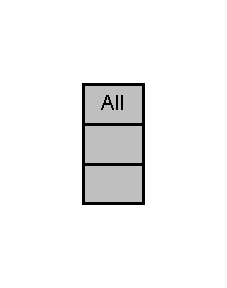
\includegraphics[width=109pt]{d3/d22/classAll__coll__graph}
\end{center}
\end{figure}


\subsection{Detailed Description}
\begin{DoxyAuthor}{Author}
silas \& louis cannot parsed into other tables. 
\end{DoxyAuthor}


The documentation for this class was generated from the following file\+:\begin{DoxyCompactItemize}
\item 
/home/silas/\+Idea\+Projects/\+En\+Ocean/src/ch/bfh/gr33nopo55um/enocean/telegram/{\bf Dummy.\+java}\end{DoxyCompactItemize}

\section{An}
\label{classAn}\index{An@{An}}


Collaboration diagram for An\+:\nopagebreak
\begin{figure}[H]
\begin{center}
\leavevmode
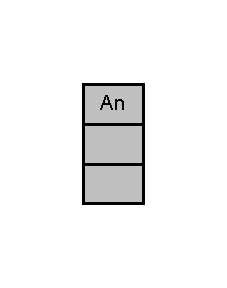
\includegraphics[width=109pt]{d8/d66/classAn__coll__graph}
\end{center}
\end{figure}


\subsection{Detailed Description}
\begin{DoxyAuthor}{Author}
silas \& louis primarily a confirmation for processes and procedures, incl. specific data content. For further informations check Enocean\+Serial\+Protocol v3 
\end{DoxyAuthor}


The documentation for this class was generated from the following file\+:\begin{DoxyCompactItemize}
\item 
/home/silas/\+Idea\+Projects/\+En\+Ocean/src/ch/bfh/gr33nopo55um/enocean/telegram/{\bf Event.\+java}\end{DoxyCompactItemize}

\section{Application}
\label{classch_1_1bfh_1_1gr33nopo55um_1_1enocean_1_1application_1_1Application}\index{Application@{Application}}


Collaboration diagram for Application\+:\nopagebreak
\begin{figure}[H]
\begin{center}
\leavevmode
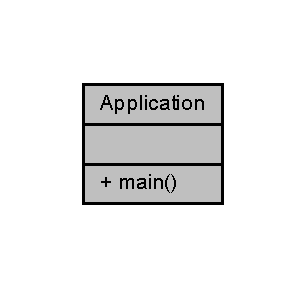
\includegraphics[width=147pt]{d2/d6b/classch_1_1bfh_1_1gr33nopo55um_1_1enocean_1_1application_1_1Application__coll__graph}
\end{center}
\end{figure}
\subsection*{Static Public Member Functions}
\begin{DoxyCompactItemize}
\item 
static void {\bf main} (String args[$\,$])  throws Exception 
\end{DoxyCompactItemize}


\subsection{Detailed Description}


Definition at line {\bf 7} of file {\bf Application.\+java}.



\subsection{Member Function Documentation}
\label{classch_1_1bfh_1_1gr33nopo55um_1_1enocean_1_1application_1_1Application_a75988cf84fc6ee7a2ebff36e363021aa} 
\index{ch\+::bfh\+::gr33nopo55um\+::enocean\+::application\+::\+Application@{ch\+::bfh\+::gr33nopo55um\+::enocean\+::application\+::\+Application}!main@{main}}
\index{main@{main}!ch\+::bfh\+::gr33nopo55um\+::enocean\+::application\+::\+Application@{ch\+::bfh\+::gr33nopo55um\+::enocean\+::application\+::\+Application}}
\subsubsection{main()}
{\footnotesize\ttfamily static void main (\begin{DoxyParamCaption}\item[{String}]{args[$\,$] }\end{DoxyParamCaption}) throws Exception\hspace{0.3cm}{\ttfamily [static]}}



Definition at line {\bf 9} of file {\bf Application.\+java}.



The documentation for this class was generated from the following file\+:\begin{DoxyCompactItemize}
\item 
/home/silas/\+Idea\+Projects/\+En\+Ocean/src/ch/bfh/gr33nopo55um/enocean/application/{\bf Application.\+java}\end{DoxyCompactItemize}

\section{Checksum}
\label{classChecksum}\index{Checksum@{Checksum}}


Collaboration diagram for Checksum\+:\nopagebreak
\begin{figure}[H]
\begin{center}
\leavevmode
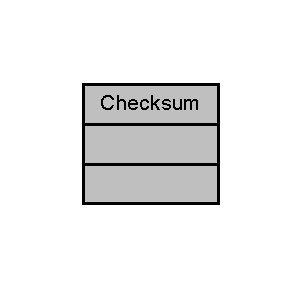
\includegraphics[width=145pt]{d0/d7c/classChecksum__coll__graph}
\end{center}
\end{figure}


\subsection{Detailed Description}
\begin{DoxyAuthor}{Author}
silas 
\end{DoxyAuthor}


The documentation for this class was generated from the following file\+:\begin{DoxyCompactItemize}
\item 
/home/silas/\+Idea\+Projects/\+En\+Ocean/src/ch/bfh/gr33nopo55um/enocean/helper/{\bf C\+R\+C.\+java}\end{DoxyCompactItemize}

\section{Class}
\label{classClass}\index{Class@{Class}}


Collaboration diagram for Class\+:\nopagebreak
\begin{figure}[H]
\begin{center}
\leavevmode
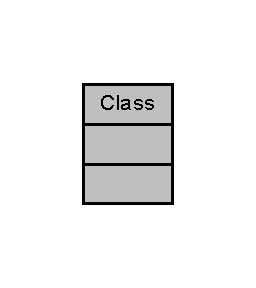
\includegraphics[width=123pt]{d2/d45/classClass__coll__graph}
\end{center}
\end{figure}


\subsection{Detailed Description}
\begin{DoxyAuthor}{Author}
silas the config file 
\end{DoxyAuthor}


The documentation for this class was generated from the following file\+:\begin{DoxyCompactItemize}
\item 
/home/silas/\+Idea\+Projects/\+En\+Ocean/src/ch/bfh/gr33nopo55um/enocean/helper/{\bf Read\+Config.\+java}\end{DoxyCompactItemize}

\section{Class}
\label{classClass}\index{Class@{Class}}


Collaboration diagram for Class\+:\nopagebreak
\begin{figure}[H]
\begin{center}
\leavevmode
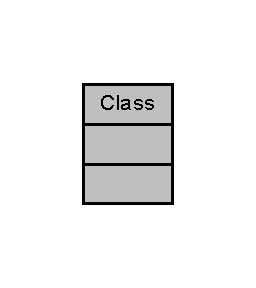
\includegraphics[width=123pt]{d2/d45/classClass__coll__graph}
\end{center}
\end{figure}


\subsection{Detailed Description}
\begin{DoxyAuthor}{Author}
silas the config file 
\end{DoxyAuthor}


The documentation for this class was generated from the following file\+:\begin{DoxyCompactItemize}
\item 
/home/silas/\+Idea\+Projects/\+En\+Ocean/src/ch/bfh/gr33nopo55um/enocean/helper/{\bf Read\+Config.\+java}\end{DoxyCompactItemize}

\section{Common\+Command}
\label{classch_1_1bfh_1_1gr33nopo55um_1_1enocean_1_1telegram_1_1CommonCommand}\index{Common\+Command@{Common\+Command}}


Inheritance diagram for Common\+Command\+:\nopagebreak
\begin{figure}[H]
\begin{center}
\leavevmode
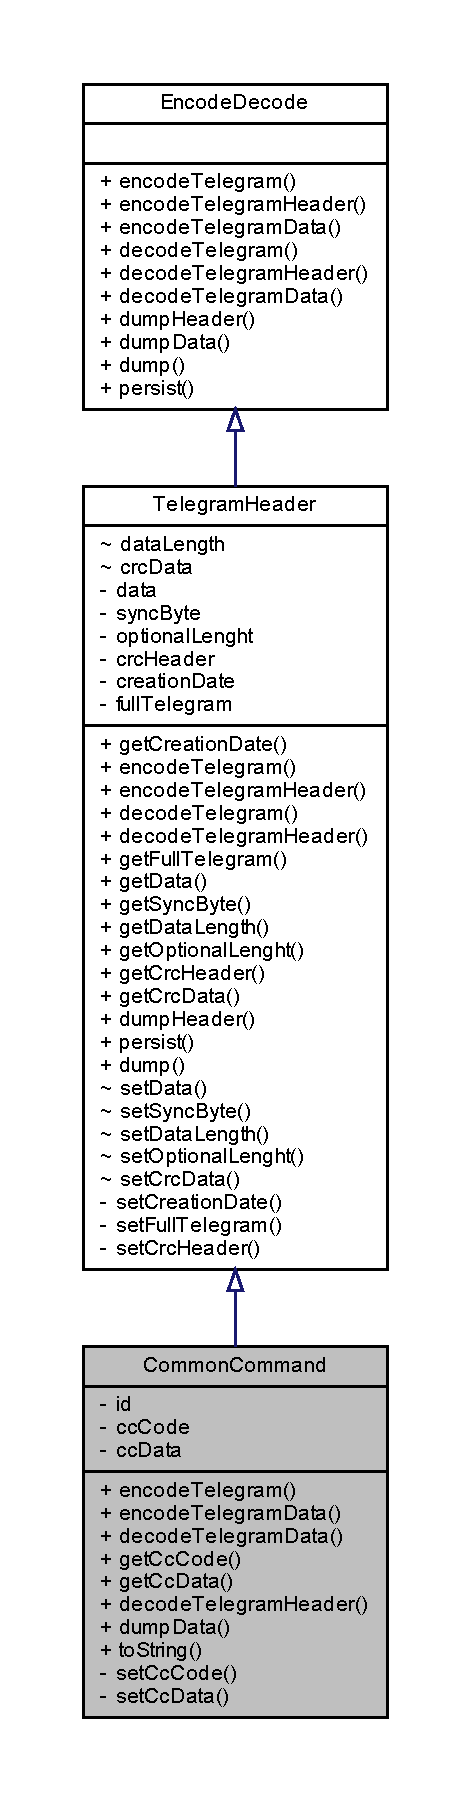
\includegraphics[height=550pt]{da/d47/classch_1_1bfh_1_1gr33nopo55um_1_1enocean_1_1telegram_1_1CommonCommand__inherit__graph}
\end{center}
\end{figure}


Collaboration diagram for Common\+Command\+:\nopagebreak
\begin{figure}[H]
\begin{center}
\leavevmode
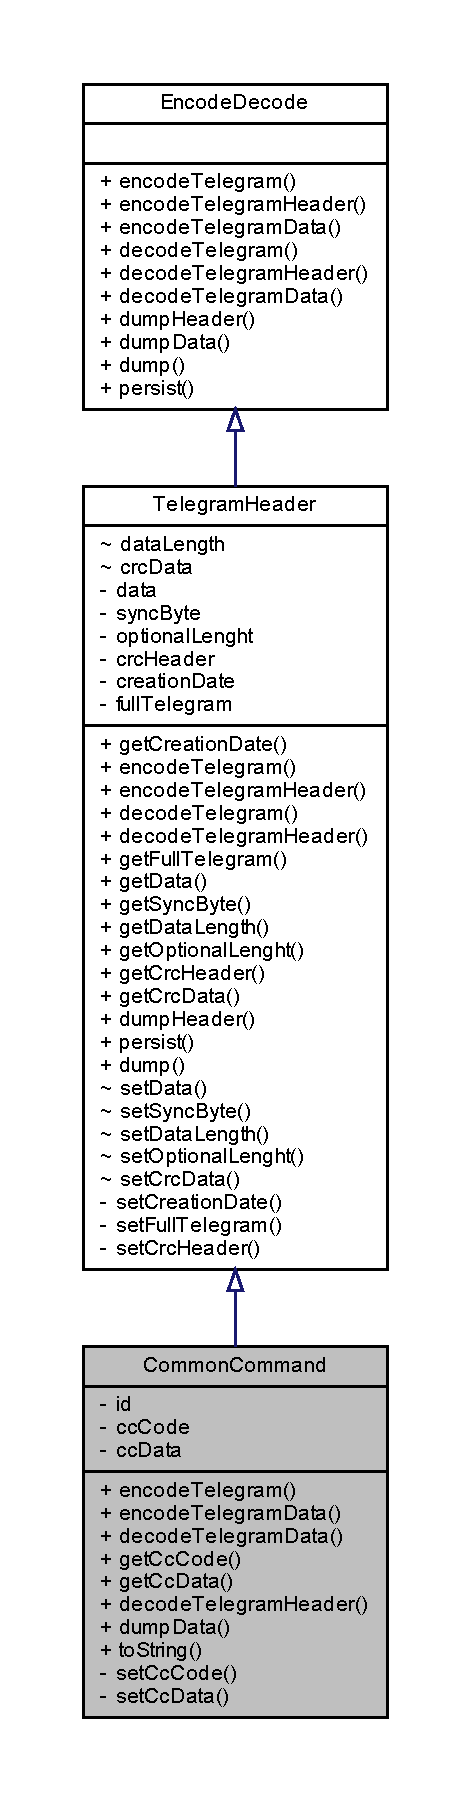
\includegraphics[height=550pt]{db/dee/classch_1_1bfh_1_1gr33nopo55um_1_1enocean_1_1telegram_1_1CommonCommand__coll__graph}
\end{center}
\end{figure}
\subsection*{Public Member Functions}
\begin{DoxyCompactItemize}
\item 
String {\bf encode\+Telegram} ()
\begin{DoxyCompactList}\small\item\em encode\+Telegram provides an example telegram hex for this packet type. \end{DoxyCompactList}\item 
String {\bf encode\+Telegram\+Data} ()
\begin{DoxyCompactList}\small\item\em encode\+Telegram\+Data provides an example data hex for this packet type. \end{DoxyCompactList}\item 
void {\bf decode\+Telegram\+Data} (String hex\+Telegram)
\begin{DoxyCompactList}\small\item\em decode\+Telegram\+Data splits telegram data in parts \end{DoxyCompactList}\item 
int {\bf get\+Cc\+Code} ()
\item 
int {\bf get\+Cc\+Data} ()
\item 
void {\bf decode\+Telegram\+Header} (String hex\+Telegram)
\item 
void {\bf dump\+Data} ()
\begin{DoxyCompactList}\small\item\em dump\+Data Print Data, useful for logs and testing En\+Ocean Telegram \end{DoxyCompactList}\item 
String {\bf to\+String} ()
\end{DoxyCompactItemize}
\subsection*{Private Member Functions}
\begin{DoxyCompactItemize}
\item 
void {\bf set\+Cc\+Code} (int {\bf cc\+Code})
\item 
void {\bf set\+Cc\+Data} (int {\bf cc\+Data})
\end{DoxyCompactItemize}
\subsection*{Private Attributes}
\begin{DoxyCompactItemize}
\item 
Long {\bf id}
\item 
int {\bf cc\+Code}
\item 
int {\bf cc\+Data}
\end{DoxyCompactItemize}
\subsection*{Additional Inherited Members}


\subsection{Detailed Description}


Definition at line {\bf 14} of file {\bf Common\+Command.\+java}.



\subsection{Member Function Documentation}
\label{classch_1_1bfh_1_1gr33nopo55um_1_1enocean_1_1telegram_1_1CommonCommand_aa581cac5c3efd3142ffa8482079031e9} 
\index{ch\+::bfh\+::gr33nopo55um\+::enocean\+::telegram\+::\+Common\+Command@{ch\+::bfh\+::gr33nopo55um\+::enocean\+::telegram\+::\+Common\+Command}!decode\+Telegram\+Data@{decode\+Telegram\+Data}}
\index{decode\+Telegram\+Data@{decode\+Telegram\+Data}!ch\+::bfh\+::gr33nopo55um\+::enocean\+::telegram\+::\+Common\+Command@{ch\+::bfh\+::gr33nopo55um\+::enocean\+::telegram\+::\+Common\+Command}}
\subsubsection{decode\+Telegram\+Data()}
{\footnotesize\ttfamily void decode\+Telegram\+Data (\begin{DoxyParamCaption}\item[{String}]{hex\+Telegram }\end{DoxyParamCaption})}



decode\+Telegram\+Data splits telegram data in parts 


\begin{DoxyParams}{Parameters}
{\em hex\+Telegram} & En\+Ocean Telegram \\
\hline
\end{DoxyParams}


Implements {\bf Encode\+Decode} \doxyref{}{p.}{d1/d8c/interfacech_1_1bfh_1_1gr33nopo55um_1_1enocean_1_1telegram_1_1EncodeDecode_aa581cac5c3efd3142ffa8482079031e9}.



Definition at line {\bf 40} of file {\bf Common\+Command.\+java}.

Here is the call graph for this function\+:\nopagebreak
\begin{figure}[H]
\begin{center}
\leavevmode
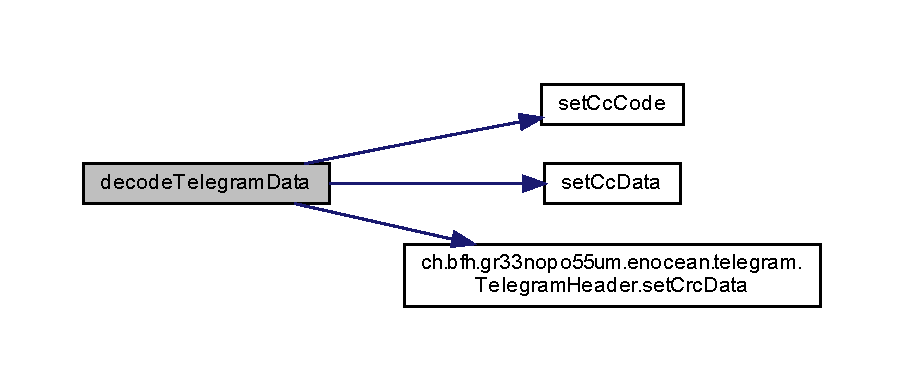
\includegraphics[width=350pt]{d6/d3b/classch_1_1bfh_1_1gr33nopo55um_1_1enocean_1_1telegram_1_1CommonCommand_aa581cac5c3efd3142ffa8482079031e9_cgraph}
\end{center}
\end{figure}
\label{classch_1_1bfh_1_1gr33nopo55um_1_1enocean_1_1telegram_1_1CommonCommand_a5e4622b1b692320953715a4f2dc064aa} 
\index{ch\+::bfh\+::gr33nopo55um\+::enocean\+::telegram\+::\+Common\+Command@{ch\+::bfh\+::gr33nopo55um\+::enocean\+::telegram\+::\+Common\+Command}!decode\+Telegram\+Header@{decode\+Telegram\+Header}}
\index{decode\+Telegram\+Header@{decode\+Telegram\+Header}!ch\+::bfh\+::gr33nopo55um\+::enocean\+::telegram\+::\+Common\+Command@{ch\+::bfh\+::gr33nopo55um\+::enocean\+::telegram\+::\+Common\+Command}}
\subsubsection{decode\+Telegram\+Header()}
{\footnotesize\ttfamily void decode\+Telegram\+Header (\begin{DoxyParamCaption}\item[{String}]{hex\+Telegram }\end{DoxyParamCaption})}

decode\+Header\+Telegram splits telegram in parts


\begin{DoxyParams}{Parameters}
{\em hex\+Telegram} & En\+Ocean Telegram \\
\hline
\end{DoxyParams}


Implements {\bf Encode\+Decode} \doxyref{}{p.}{d1/d8c/interfacech_1_1bfh_1_1gr33nopo55um_1_1enocean_1_1telegram_1_1EncodeDecode_a5e4622b1b692320953715a4f2dc064aa}.



Definition at line {\bf 71} of file {\bf Common\+Command.\+java}.

\label{classch_1_1bfh_1_1gr33nopo55um_1_1enocean_1_1telegram_1_1CommonCommand_aff152c0c0c3d5e7011bfff0b9c08032b} 
\index{ch\+::bfh\+::gr33nopo55um\+::enocean\+::telegram\+::\+Common\+Command@{ch\+::bfh\+::gr33nopo55um\+::enocean\+::telegram\+::\+Common\+Command}!dump\+Data@{dump\+Data}}
\index{dump\+Data@{dump\+Data}!ch\+::bfh\+::gr33nopo55um\+::enocean\+::telegram\+::\+Common\+Command@{ch\+::bfh\+::gr33nopo55um\+::enocean\+::telegram\+::\+Common\+Command}}
\subsubsection{dump\+Data()}
{\footnotesize\ttfamily void dump\+Data (\begin{DoxyParamCaption}{ }\end{DoxyParamCaption})}



dump\+Data Print Data, useful for logs and testing En\+Ocean Telegram 



Implements {\bf Encode\+Decode} \doxyref{}{p.}{d1/d8c/interfacech_1_1bfh_1_1gr33nopo55um_1_1enocean_1_1telegram_1_1EncodeDecode_aff152c0c0c3d5e7011bfff0b9c08032b}.



Definition at line {\bf 79} of file {\bf Common\+Command.\+java}.

Here is the call graph for this function\+:\nopagebreak
\begin{figure}[H]
\begin{center}
\leavevmode
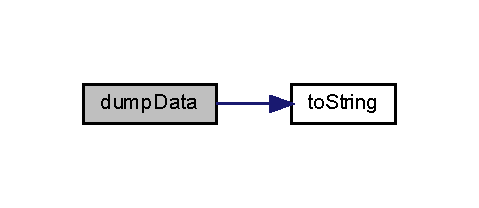
\includegraphics[width=230pt]{d6/d3b/classch_1_1bfh_1_1gr33nopo55um_1_1enocean_1_1telegram_1_1CommonCommand_aff152c0c0c3d5e7011bfff0b9c08032b_cgraph}
\end{center}
\end{figure}
\label{classch_1_1bfh_1_1gr33nopo55um_1_1enocean_1_1telegram_1_1CommonCommand_a00e3ee3b777334ef3bd46bd4105f9603} 
\index{ch\+::bfh\+::gr33nopo55um\+::enocean\+::telegram\+::\+Common\+Command@{ch\+::bfh\+::gr33nopo55um\+::enocean\+::telegram\+::\+Common\+Command}!encode\+Telegram@{encode\+Telegram}}
\index{encode\+Telegram@{encode\+Telegram}!ch\+::bfh\+::gr33nopo55um\+::enocean\+::telegram\+::\+Common\+Command@{ch\+::bfh\+::gr33nopo55um\+::enocean\+::telegram\+::\+Common\+Command}}
\subsubsection{encode\+Telegram()}
{\footnotesize\ttfamily String encode\+Telegram (\begin{DoxyParamCaption}{ }\end{DoxyParamCaption})}



encode\+Telegram provides an example telegram hex for this packet type. 

\begin{DoxyReturn}{Returns}
String hex\+Telegram En\+Ocean Telegram 
\end{DoxyReturn}


Implements {\bf Encode\+Decode} \doxyref{}{p.}{d1/d8c/interfacech_1_1bfh_1_1gr33nopo55um_1_1enocean_1_1telegram_1_1EncodeDecode_a00e3ee3b777334ef3bd46bd4105f9603}.



Definition at line {\bf 26} of file {\bf Common\+Command.\+java}.

\label{classch_1_1bfh_1_1gr33nopo55um_1_1enocean_1_1telegram_1_1CommonCommand_a8a67618ab0362f3d0b60bba6ca93d883} 
\index{ch\+::bfh\+::gr33nopo55um\+::enocean\+::telegram\+::\+Common\+Command@{ch\+::bfh\+::gr33nopo55um\+::enocean\+::telegram\+::\+Common\+Command}!encode\+Telegram\+Data@{encode\+Telegram\+Data}}
\index{encode\+Telegram\+Data@{encode\+Telegram\+Data}!ch\+::bfh\+::gr33nopo55um\+::enocean\+::telegram\+::\+Common\+Command@{ch\+::bfh\+::gr33nopo55um\+::enocean\+::telegram\+::\+Common\+Command}}
\subsubsection{encode\+Telegram\+Data()}
{\footnotesize\ttfamily String encode\+Telegram\+Data (\begin{DoxyParamCaption}{ }\end{DoxyParamCaption})}



encode\+Telegram\+Data provides an example data hex for this packet type. 

\begin{DoxyReturn}{Returns}
String hex\+Telegram\+Data En\+Ocean Telegram 
\end{DoxyReturn}


Implements {\bf Encode\+Decode} \doxyref{}{p.}{d1/d8c/interfacech_1_1bfh_1_1gr33nopo55um_1_1enocean_1_1telegram_1_1EncodeDecode_a8a67618ab0362f3d0b60bba6ca93d883}.



Definition at line {\bf 35} of file {\bf Common\+Command.\+java}.

\label{classch_1_1bfh_1_1gr33nopo55um_1_1enocean_1_1telegram_1_1CommonCommand_a2612bb827975ffc5433e75572a235617} 
\index{ch\+::bfh\+::gr33nopo55um\+::enocean\+::telegram\+::\+Common\+Command@{ch\+::bfh\+::gr33nopo55um\+::enocean\+::telegram\+::\+Common\+Command}!get\+Cc\+Code@{get\+Cc\+Code}}
\index{get\+Cc\+Code@{get\+Cc\+Code}!ch\+::bfh\+::gr33nopo55um\+::enocean\+::telegram\+::\+Common\+Command@{ch\+::bfh\+::gr33nopo55um\+::enocean\+::telegram\+::\+Common\+Command}}
\subsubsection{get\+Cc\+Code()}
{\footnotesize\ttfamily int get\+Cc\+Code (\begin{DoxyParamCaption}{ }\end{DoxyParamCaption})}



Definition at line {\bf 49} of file {\bf Common\+Command.\+java}.

\label{classch_1_1bfh_1_1gr33nopo55um_1_1enocean_1_1telegram_1_1CommonCommand_a70e53361247650ffacb77157cf6367dc} 
\index{ch\+::bfh\+::gr33nopo55um\+::enocean\+::telegram\+::\+Common\+Command@{ch\+::bfh\+::gr33nopo55um\+::enocean\+::telegram\+::\+Common\+Command}!get\+Cc\+Data@{get\+Cc\+Data}}
\index{get\+Cc\+Data@{get\+Cc\+Data}!ch\+::bfh\+::gr33nopo55um\+::enocean\+::telegram\+::\+Common\+Command@{ch\+::bfh\+::gr33nopo55um\+::enocean\+::telegram\+::\+Common\+Command}}
\subsubsection{get\+Cc\+Data()}
{\footnotesize\ttfamily int get\+Cc\+Data (\begin{DoxyParamCaption}{ }\end{DoxyParamCaption})}



Definition at line {\bf 57} of file {\bf Common\+Command.\+java}.

\label{classch_1_1bfh_1_1gr33nopo55um_1_1enocean_1_1telegram_1_1CommonCommand_ac65886e1c8ef317295d9dcd82f700b95} 
\index{ch\+::bfh\+::gr33nopo55um\+::enocean\+::telegram\+::\+Common\+Command@{ch\+::bfh\+::gr33nopo55um\+::enocean\+::telegram\+::\+Common\+Command}!set\+Cc\+Code@{set\+Cc\+Code}}
\index{set\+Cc\+Code@{set\+Cc\+Code}!ch\+::bfh\+::gr33nopo55um\+::enocean\+::telegram\+::\+Common\+Command@{ch\+::bfh\+::gr33nopo55um\+::enocean\+::telegram\+::\+Common\+Command}}
\subsubsection{set\+Cc\+Code()}
{\footnotesize\ttfamily void set\+Cc\+Code (\begin{DoxyParamCaption}\item[{int}]{cc\+Code }\end{DoxyParamCaption})\hspace{0.3cm}{\ttfamily [private]}}



Definition at line {\bf 53} of file {\bf Common\+Command.\+java}.

Here is the caller graph for this function\+:\nopagebreak
\begin{figure}[H]
\begin{center}
\leavevmode
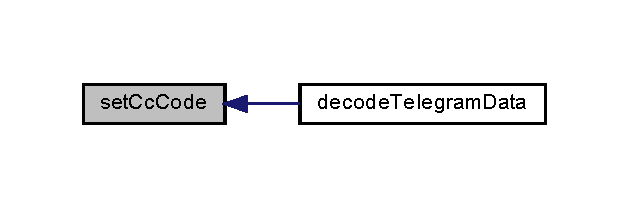
\includegraphics[width=302pt]{d6/d3b/classch_1_1bfh_1_1gr33nopo55um_1_1enocean_1_1telegram_1_1CommonCommand_ac65886e1c8ef317295d9dcd82f700b95_icgraph}
\end{center}
\end{figure}
\label{classch_1_1bfh_1_1gr33nopo55um_1_1enocean_1_1telegram_1_1CommonCommand_aa785ba47d3c242d27b6ff3b93864ec1a} 
\index{ch\+::bfh\+::gr33nopo55um\+::enocean\+::telegram\+::\+Common\+Command@{ch\+::bfh\+::gr33nopo55um\+::enocean\+::telegram\+::\+Common\+Command}!set\+Cc\+Data@{set\+Cc\+Data}}
\index{set\+Cc\+Data@{set\+Cc\+Data}!ch\+::bfh\+::gr33nopo55um\+::enocean\+::telegram\+::\+Common\+Command@{ch\+::bfh\+::gr33nopo55um\+::enocean\+::telegram\+::\+Common\+Command}}
\subsubsection{set\+Cc\+Data()}
{\footnotesize\ttfamily void set\+Cc\+Data (\begin{DoxyParamCaption}\item[{int}]{cc\+Data }\end{DoxyParamCaption})\hspace{0.3cm}{\ttfamily [private]}}



Definition at line {\bf 61} of file {\bf Common\+Command.\+java}.

Here is the caller graph for this function\+:\nopagebreak
\begin{figure}[H]
\begin{center}
\leavevmode
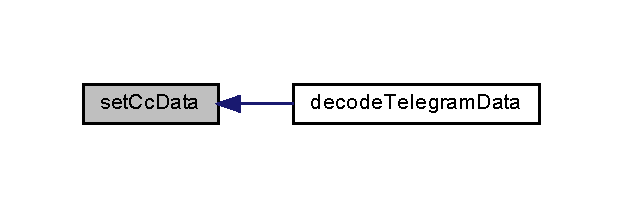
\includegraphics[width=299pt]{d6/d3b/classch_1_1bfh_1_1gr33nopo55um_1_1enocean_1_1telegram_1_1CommonCommand_aa785ba47d3c242d27b6ff3b93864ec1a_icgraph}
\end{center}
\end{figure}
\label{classch_1_1bfh_1_1gr33nopo55um_1_1enocean_1_1telegram_1_1CommonCommand_ad146fa8579a5f8a876c4688cc5a68520} 
\index{ch\+::bfh\+::gr33nopo55um\+::enocean\+::telegram\+::\+Common\+Command@{ch\+::bfh\+::gr33nopo55um\+::enocean\+::telegram\+::\+Common\+Command}!to\+String@{to\+String}}
\index{to\+String@{to\+String}!ch\+::bfh\+::gr33nopo55um\+::enocean\+::telegram\+::\+Common\+Command@{ch\+::bfh\+::gr33nopo55um\+::enocean\+::telegram\+::\+Common\+Command}}
\subsubsection{to\+String()}
{\footnotesize\ttfamily String to\+String (\begin{DoxyParamCaption}{ }\end{DoxyParamCaption})}



Definition at line {\bf 86} of file {\bf Common\+Command.\+java}.

Here is the caller graph for this function\+:\nopagebreak
\begin{figure}[H]
\begin{center}
\leavevmode
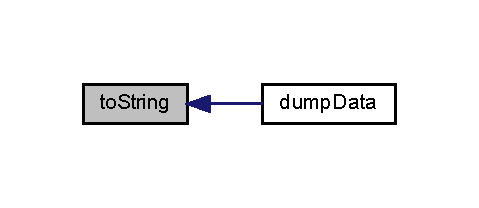
\includegraphics[width=230pt]{d6/d3b/classch_1_1bfh_1_1gr33nopo55um_1_1enocean_1_1telegram_1_1CommonCommand_ad146fa8579a5f8a876c4688cc5a68520_icgraph}
\end{center}
\end{figure}


\subsection{Member Data Documentation}
\label{classch_1_1bfh_1_1gr33nopo55um_1_1enocean_1_1telegram_1_1CommonCommand_a1216041344f882e7d38ab7250f551089} 
\index{ch\+::bfh\+::gr33nopo55um\+::enocean\+::telegram\+::\+Common\+Command@{ch\+::bfh\+::gr33nopo55um\+::enocean\+::telegram\+::\+Common\+Command}!cc\+Code@{cc\+Code}}
\index{cc\+Code@{cc\+Code}!ch\+::bfh\+::gr33nopo55um\+::enocean\+::telegram\+::\+Common\+Command@{ch\+::bfh\+::gr33nopo55um\+::enocean\+::telegram\+::\+Common\+Command}}
\subsubsection{cc\+Code}
{\footnotesize\ttfamily int cc\+Code\hspace{0.3cm}{\ttfamily [private]}}



Definition at line {\bf 22} of file {\bf Common\+Command.\+java}.

\label{classch_1_1bfh_1_1gr33nopo55um_1_1enocean_1_1telegram_1_1CommonCommand_a66f5a22806d676a1aba22f5347ef2689} 
\index{ch\+::bfh\+::gr33nopo55um\+::enocean\+::telegram\+::\+Common\+Command@{ch\+::bfh\+::gr33nopo55um\+::enocean\+::telegram\+::\+Common\+Command}!cc\+Data@{cc\+Data}}
\index{cc\+Data@{cc\+Data}!ch\+::bfh\+::gr33nopo55um\+::enocean\+::telegram\+::\+Common\+Command@{ch\+::bfh\+::gr33nopo55um\+::enocean\+::telegram\+::\+Common\+Command}}
\subsubsection{cc\+Data}
{\footnotesize\ttfamily int cc\+Data\hspace{0.3cm}{\ttfamily [private]}}



Definition at line {\bf 23} of file {\bf Common\+Command.\+java}.

\label{classch_1_1bfh_1_1gr33nopo55um_1_1enocean_1_1telegram_1_1CommonCommand_afdea3f4ac85ac5819c978584be2be48e} 
\index{ch\+::bfh\+::gr33nopo55um\+::enocean\+::telegram\+::\+Common\+Command@{ch\+::bfh\+::gr33nopo55um\+::enocean\+::telegram\+::\+Common\+Command}!id@{id}}
\index{id@{id}!ch\+::bfh\+::gr33nopo55um\+::enocean\+::telegram\+::\+Common\+Command@{ch\+::bfh\+::gr33nopo55um\+::enocean\+::telegram\+::\+Common\+Command}}
\subsubsection{id}
{\footnotesize\ttfamily Long id\hspace{0.3cm}{\ttfamily [private]}}



Definition at line {\bf 19} of file {\bf Common\+Command.\+java}.



The documentation for this class was generated from the following file\+:\begin{DoxyCompactItemize}
\item 
/home/silas/\+Idea\+Projects/\+En\+Ocean/src/ch/bfh/gr33nopo55um/enocean/telegram/{\bf Common\+Command.\+java}\end{DoxyCompactItemize}

\section{C\+RC}
\label{classch_1_1bfh_1_1gr33nopo55um_1_1enocean_1_1helper_1_1CRC}\index{C\+RC@{C\+RC}}


Collaboration diagram for C\+RC\+:\nopagebreak
\begin{figure}[H]
\begin{center}
\leavevmode
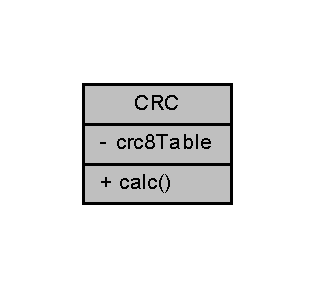
\includegraphics[width=151pt]{d2/df5/classch_1_1bfh_1_1gr33nopo55um_1_1enocean_1_1helper_1_1CRC__coll__graph}
\end{center}
\end{figure}
\subsection*{Static Public Member Functions}
\begin{DoxyCompactItemize}
\item 
static byte {\bf calc} (byte[$\,$] data)
\end{DoxyCompactItemize}
\subsection*{Static Private Attributes}
\begin{DoxyCompactItemize}
\item 
static byte [$\,$] {\bf crc8\+Table}
\end{DoxyCompactItemize}


\subsection{Detailed Description}


Definition at line {\bf 8} of file {\bf C\+R\+C.\+java}.



\subsection{Member Function Documentation}
\label{classch_1_1bfh_1_1gr33nopo55um_1_1enocean_1_1helper_1_1CRC_a637a5507ae52f99f1326f24dacb3e454} 
\index{ch\+::bfh\+::gr33nopo55um\+::enocean\+::helper\+::\+C\+RC@{ch\+::bfh\+::gr33nopo55um\+::enocean\+::helper\+::\+C\+RC}!calc@{calc}}
\index{calc@{calc}!ch\+::bfh\+::gr33nopo55um\+::enocean\+::helper\+::\+C\+RC@{ch\+::bfh\+::gr33nopo55um\+::enocean\+::helper\+::\+C\+RC}}
\subsubsection{calc()}
{\footnotesize\ttfamily static byte calc (\begin{DoxyParamCaption}\item[{byte [$\,$]}]{data }\end{DoxyParamCaption})\hspace{0.3cm}{\ttfamily [static]}}



Definition at line {\bf 44} of file {\bf C\+R\+C.\+java}.



\subsection{Member Data Documentation}
\label{classch_1_1bfh_1_1gr33nopo55um_1_1enocean_1_1helper_1_1CRC_a3e402bbcde6dc6c78939936f69c8f963} 
\index{ch\+::bfh\+::gr33nopo55um\+::enocean\+::helper\+::\+C\+RC@{ch\+::bfh\+::gr33nopo55um\+::enocean\+::helper\+::\+C\+RC}!crc8\+Table@{crc8\+Table}}
\index{crc8\+Table@{crc8\+Table}!ch\+::bfh\+::gr33nopo55um\+::enocean\+::helper\+::\+C\+RC@{ch\+::bfh\+::gr33nopo55um\+::enocean\+::helper\+::\+C\+RC}}
\subsubsection{crc8\+Table}
{\footnotesize\ttfamily byte [$\,$] crc8\+Table\hspace{0.3cm}{\ttfamily [static]}, {\ttfamily [private]}}



Definition at line {\bf 10} of file {\bf C\+R\+C.\+java}.



The documentation for this class was generated from the following file\+:\begin{DoxyCompactItemize}
\item 
/home/silas/\+Idea\+Projects/\+En\+Ocean/src/ch/bfh/gr33nopo55um/enocean/helper/{\bf C\+R\+C.\+java}\end{DoxyCompactItemize}

\section{DB}
\label{classDB}\index{DB@{DB}}


Collaboration diagram for DB\+:\nopagebreak
\begin{figure}[H]
\begin{center}
\leavevmode
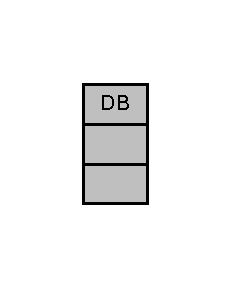
\includegraphics[width=111pt]{d7/d82/classDB__coll__graph}
\end{center}
\end{figure}


\subsection{Detailed Description}
inital gnerating

\begin{DoxyAuthor}{Author}
silas 
\end{DoxyAuthor}


The documentation for this class was generated from the following file\+:\begin{DoxyCompactItemize}
\item 
/home/silas/\+Idea\+Projects/\+En\+Ocean/src/ch/bfh/gr33nopo55um/enocean/persistence/{\bf Seed\+D\+B.\+java}\end{DoxyCompactItemize}

\section{diagnosis}
\label{classdiagnosis}\index{diagnosis@{diagnosis}}


Collaboration diagram for diagnosis\+:\nopagebreak
\begin{figure}[H]
\begin{center}
\leavevmode
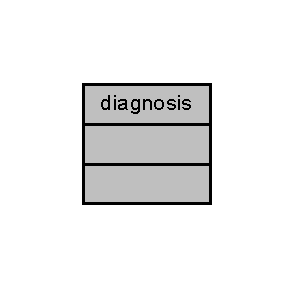
\includegraphics[width=141pt]{de/dfe/classdiagnosis__coll__graph}
\end{center}
\end{figure}


\subsection{Detailed Description}
\begin{DoxyAuthor}{Author}
silas \& louis . The packet design corresponds to the type R\+A\+D\+I\+O\+\_\+\+E\+R\+P1. The content of the O\+P\+T\+I\+O\+N\+A\+L\+\_\+\+D\+A\+TA is altered slightly, for further informations check Enocean\+Serial\+Protocol v3 
\end{DoxyAuthor}


The documentation for this class was generated from the following file\+:\begin{DoxyCompactItemize}
\item 
/home/silas/\+Idea\+Projects/\+En\+Ocean/src/ch/bfh/gr33nopo55um/enocean/telegram/{\bf Radio\+Sub\+Tel.\+java}\end{DoxyCompactItemize}

\section{Dummy}
\label{classch_1_1bfh_1_1gr33nopo55um_1_1enocean_1_1telegram_1_1Dummy}\index{Dummy@{Dummy}}


Inheritance diagram for Dummy\+:\nopagebreak
\begin{figure}[H]
\begin{center}
\leavevmode
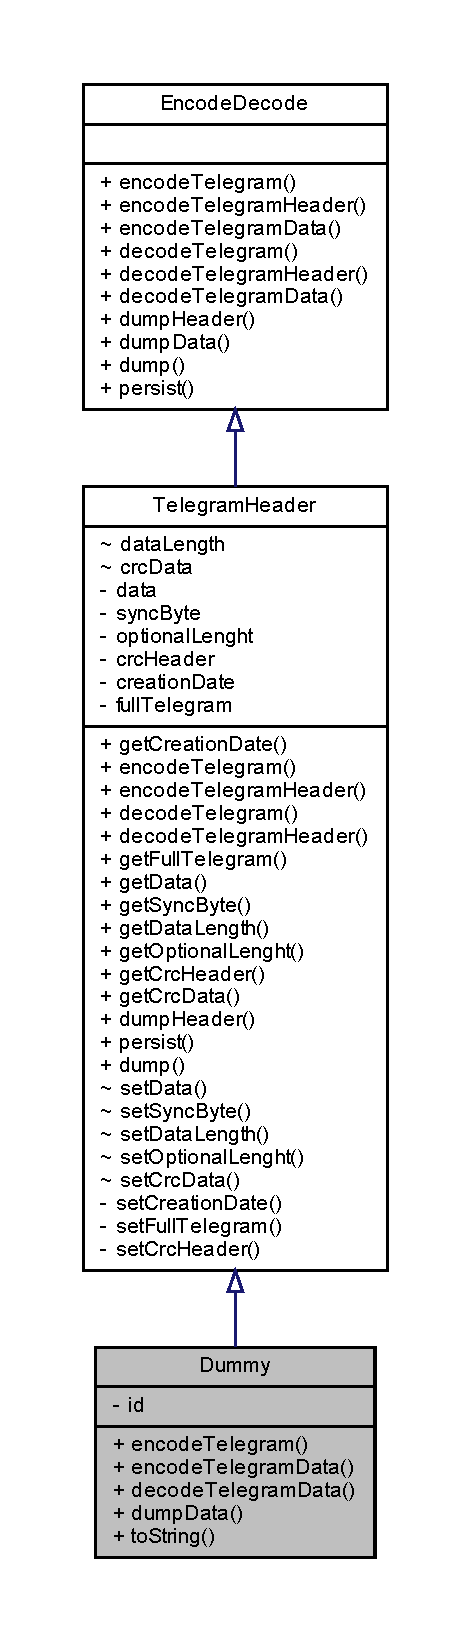
\includegraphics[height=550pt]{d2/d37/classch_1_1bfh_1_1gr33nopo55um_1_1enocean_1_1telegram_1_1Dummy__inherit__graph}
\end{center}
\end{figure}


Collaboration diagram for Dummy\+:\nopagebreak
\begin{figure}[H]
\begin{center}
\leavevmode
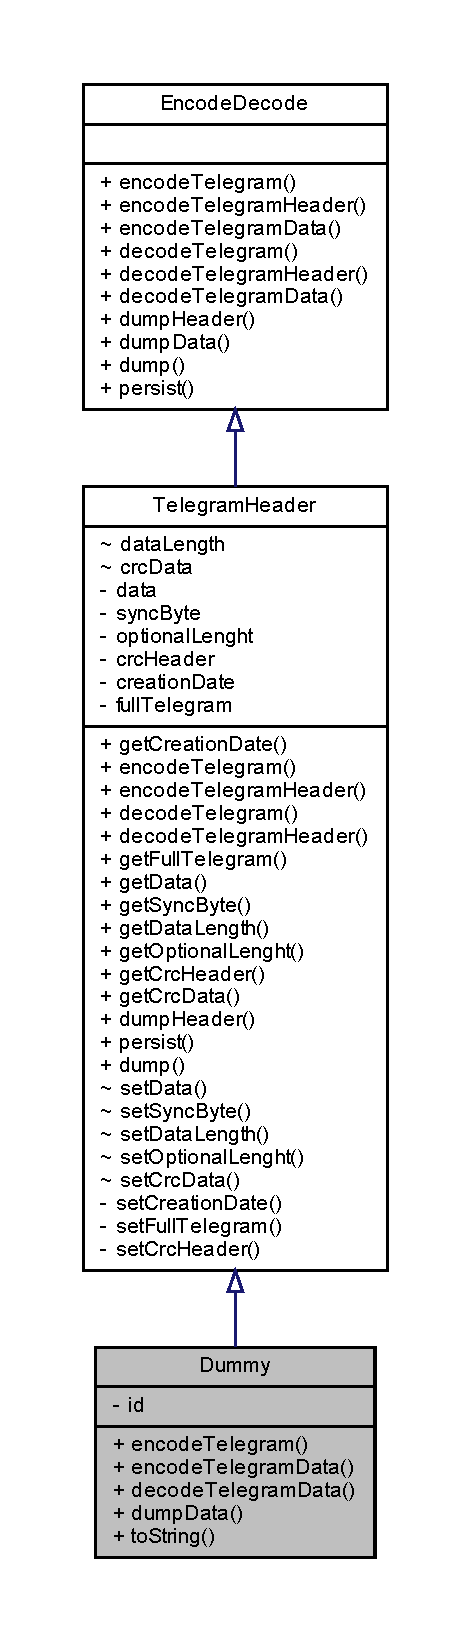
\includegraphics[height=550pt]{d0/d68/classch_1_1bfh_1_1gr33nopo55um_1_1enocean_1_1telegram_1_1Dummy__coll__graph}
\end{center}
\end{figure}
\subsection*{Public Member Functions}
\begin{DoxyCompactItemize}
\item 
String {\bf encode\+Telegram} ()
\begin{DoxyCompactList}\small\item\em encode\+Telegram provides an example telegram hex for this packet type. \end{DoxyCompactList}\item 
String {\bf encode\+Telegram\+Data} ()
\item 
void {\bf decode\+Telegram\+Data} (String hex\+Telegram)
\item 
void {\bf dump\+Data} ()
\begin{DoxyCompactList}\small\item\em usally a dummy package does not have any data \end{DoxyCompactList}\item 
String {\bf to\+String} ()
\end{DoxyCompactItemize}
\subsection*{Private Attributes}
\begin{DoxyCompactItemize}
\item 
Long {\bf id}
\end{DoxyCompactItemize}
\subsection*{Additional Inherited Members}


\subsection{Detailed Description}


Definition at line {\bf 13} of file {\bf Dummy.\+java}.



\subsection{Member Function Documentation}
\label{classch_1_1bfh_1_1gr33nopo55um_1_1enocean_1_1telegram_1_1Dummy_aa581cac5c3efd3142ffa8482079031e9} 
\index{ch\+::bfh\+::gr33nopo55um\+::enocean\+::telegram\+::\+Dummy@{ch\+::bfh\+::gr33nopo55um\+::enocean\+::telegram\+::\+Dummy}!decode\+Telegram\+Data@{decode\+Telegram\+Data}}
\index{decode\+Telegram\+Data@{decode\+Telegram\+Data}!ch\+::bfh\+::gr33nopo55um\+::enocean\+::telegram\+::\+Dummy@{ch\+::bfh\+::gr33nopo55um\+::enocean\+::telegram\+::\+Dummy}}
\subsubsection{decode\+Telegram\+Data()}
{\footnotesize\ttfamily void decode\+Telegram\+Data (\begin{DoxyParamCaption}\item[{String}]{hex\+Telegram }\end{DoxyParamCaption})}


\begin{DoxyParams}{Parameters}
{\em hex\+Telegram} & En\+Ocean Telegram \\
\hline
\end{DoxyParams}


Implements {\bf Encode\+Decode} \doxyref{}{p.}{d1/d8c/interfacech_1_1bfh_1_1gr33nopo55um_1_1enocean_1_1telegram_1_1EncodeDecode_aa581cac5c3efd3142ffa8482079031e9}.



Definition at line {\bf 40} of file {\bf Dummy.\+java}.

\label{classch_1_1bfh_1_1gr33nopo55um_1_1enocean_1_1telegram_1_1Dummy_aff152c0c0c3d5e7011bfff0b9c08032b} 
\index{ch\+::bfh\+::gr33nopo55um\+::enocean\+::telegram\+::\+Dummy@{ch\+::bfh\+::gr33nopo55um\+::enocean\+::telegram\+::\+Dummy}!dump\+Data@{dump\+Data}}
\index{dump\+Data@{dump\+Data}!ch\+::bfh\+::gr33nopo55um\+::enocean\+::telegram\+::\+Dummy@{ch\+::bfh\+::gr33nopo55um\+::enocean\+::telegram\+::\+Dummy}}
\subsubsection{dump\+Data()}
{\footnotesize\ttfamily void dump\+Data (\begin{DoxyParamCaption}{ }\end{DoxyParamCaption})}



usally a dummy package does not have any data 



Implements {\bf Encode\+Decode} \doxyref{}{p.}{d1/d8c/interfacech_1_1bfh_1_1gr33nopo55um_1_1enocean_1_1telegram_1_1EncodeDecode_aff152c0c0c3d5e7011bfff0b9c08032b}.



Definition at line {\bf 48} of file {\bf Dummy.\+java}.

\label{classch_1_1bfh_1_1gr33nopo55um_1_1enocean_1_1telegram_1_1Dummy_a00e3ee3b777334ef3bd46bd4105f9603} 
\index{ch\+::bfh\+::gr33nopo55um\+::enocean\+::telegram\+::\+Dummy@{ch\+::bfh\+::gr33nopo55um\+::enocean\+::telegram\+::\+Dummy}!encode\+Telegram@{encode\+Telegram}}
\index{encode\+Telegram@{encode\+Telegram}!ch\+::bfh\+::gr33nopo55um\+::enocean\+::telegram\+::\+Dummy@{ch\+::bfh\+::gr33nopo55um\+::enocean\+::telegram\+::\+Dummy}}
\subsubsection{encode\+Telegram()}
{\footnotesize\ttfamily String encode\+Telegram (\begin{DoxyParamCaption}{ }\end{DoxyParamCaption})}



encode\+Telegram provides an example telegram hex for this packet type. 

\begin{DoxyReturn}{Returns}
String hex\+Telegram En\+Ocean Telegram 
\end{DoxyReturn}


Implements {\bf Encode\+Decode} \doxyref{}{p.}{d1/d8c/interfacech_1_1bfh_1_1gr33nopo55um_1_1enocean_1_1telegram_1_1EncodeDecode_a00e3ee3b777334ef3bd46bd4105f9603}.



Definition at line {\bf 21} of file {\bf Dummy.\+java}.

\label{classch_1_1bfh_1_1gr33nopo55um_1_1enocean_1_1telegram_1_1Dummy_a8a67618ab0362f3d0b60bba6ca93d883} 
\index{ch\+::bfh\+::gr33nopo55um\+::enocean\+::telegram\+::\+Dummy@{ch\+::bfh\+::gr33nopo55um\+::enocean\+::telegram\+::\+Dummy}!encode\+Telegram\+Data@{encode\+Telegram\+Data}}
\index{encode\+Telegram\+Data@{encode\+Telegram\+Data}!ch\+::bfh\+::gr33nopo55um\+::enocean\+::telegram\+::\+Dummy@{ch\+::bfh\+::gr33nopo55um\+::enocean\+::telegram\+::\+Dummy}}
\subsubsection{encode\+Telegram\+Data()}
{\footnotesize\ttfamily String encode\+Telegram\+Data (\begin{DoxyParamCaption}{ }\end{DoxyParamCaption})}

encode\+Telegram\+Data provides an example data hex for this packet type.

\begin{DoxyReturn}{Returns}
String hex\+Telegram\+Data En\+Ocean Telegram 
\end{DoxyReturn}


Implements {\bf Encode\+Decode} \doxyref{}{p.}{d1/d8c/interfacech_1_1bfh_1_1gr33nopo55um_1_1enocean_1_1telegram_1_1EncodeDecode_a8a67618ab0362f3d0b60bba6ca93d883}.



Definition at line {\bf 31} of file {\bf Dummy.\+java}.

\label{classch_1_1bfh_1_1gr33nopo55um_1_1enocean_1_1telegram_1_1Dummy_ad146fa8579a5f8a876c4688cc5a68520} 
\index{ch\+::bfh\+::gr33nopo55um\+::enocean\+::telegram\+::\+Dummy@{ch\+::bfh\+::gr33nopo55um\+::enocean\+::telegram\+::\+Dummy}!to\+String@{to\+String}}
\index{to\+String@{to\+String}!ch\+::bfh\+::gr33nopo55um\+::enocean\+::telegram\+::\+Dummy@{ch\+::bfh\+::gr33nopo55um\+::enocean\+::telegram\+::\+Dummy}}
\subsubsection{to\+String()}
{\footnotesize\ttfamily String to\+String (\begin{DoxyParamCaption}{ }\end{DoxyParamCaption})}

\begin{DoxyReturn}{Returns}
Packet\+Type=\doxyref{Dummy}{p.}{d1/df6/classch_1_1bfh_1_1gr33nopo55um_1_1enocean_1_1telegram_1_1Dummy} 
\end{DoxyReturn}


Definition at line {\bf 56} of file {\bf Dummy.\+java}.



\subsection{Member Data Documentation}
\label{classch_1_1bfh_1_1gr33nopo55um_1_1enocean_1_1telegram_1_1Dummy_afdea3f4ac85ac5819c978584be2be48e} 
\index{ch\+::bfh\+::gr33nopo55um\+::enocean\+::telegram\+::\+Dummy@{ch\+::bfh\+::gr33nopo55um\+::enocean\+::telegram\+::\+Dummy}!id@{id}}
\index{id@{id}!ch\+::bfh\+::gr33nopo55um\+::enocean\+::telegram\+::\+Dummy@{ch\+::bfh\+::gr33nopo55um\+::enocean\+::telegram\+::\+Dummy}}
\subsubsection{id}
{\footnotesize\ttfamily Long id\hspace{0.3cm}{\ttfamily [private]}}



Definition at line {\bf 17} of file {\bf Dummy.\+java}.



The documentation for this class was generated from the following file\+:\begin{DoxyCompactItemize}
\item 
/home/silas/\+Idea\+Projects/\+En\+Ocean/src/ch/bfh/gr33nopo55um/enocean/telegram/{\bf Dummy.\+java}\end{DoxyCompactItemize}

\section{Encode\+Decode}
\label{interfacech_1_1bfh_1_1gr33nopo55um_1_1enocean_1_1telegram_1_1EncodeDecode}\index{Encode\+Decode@{Encode\+Decode}}


Inheritance diagram for Encode\+Decode\+:\nopagebreak
\begin{figure}[H]
\begin{center}
\leavevmode
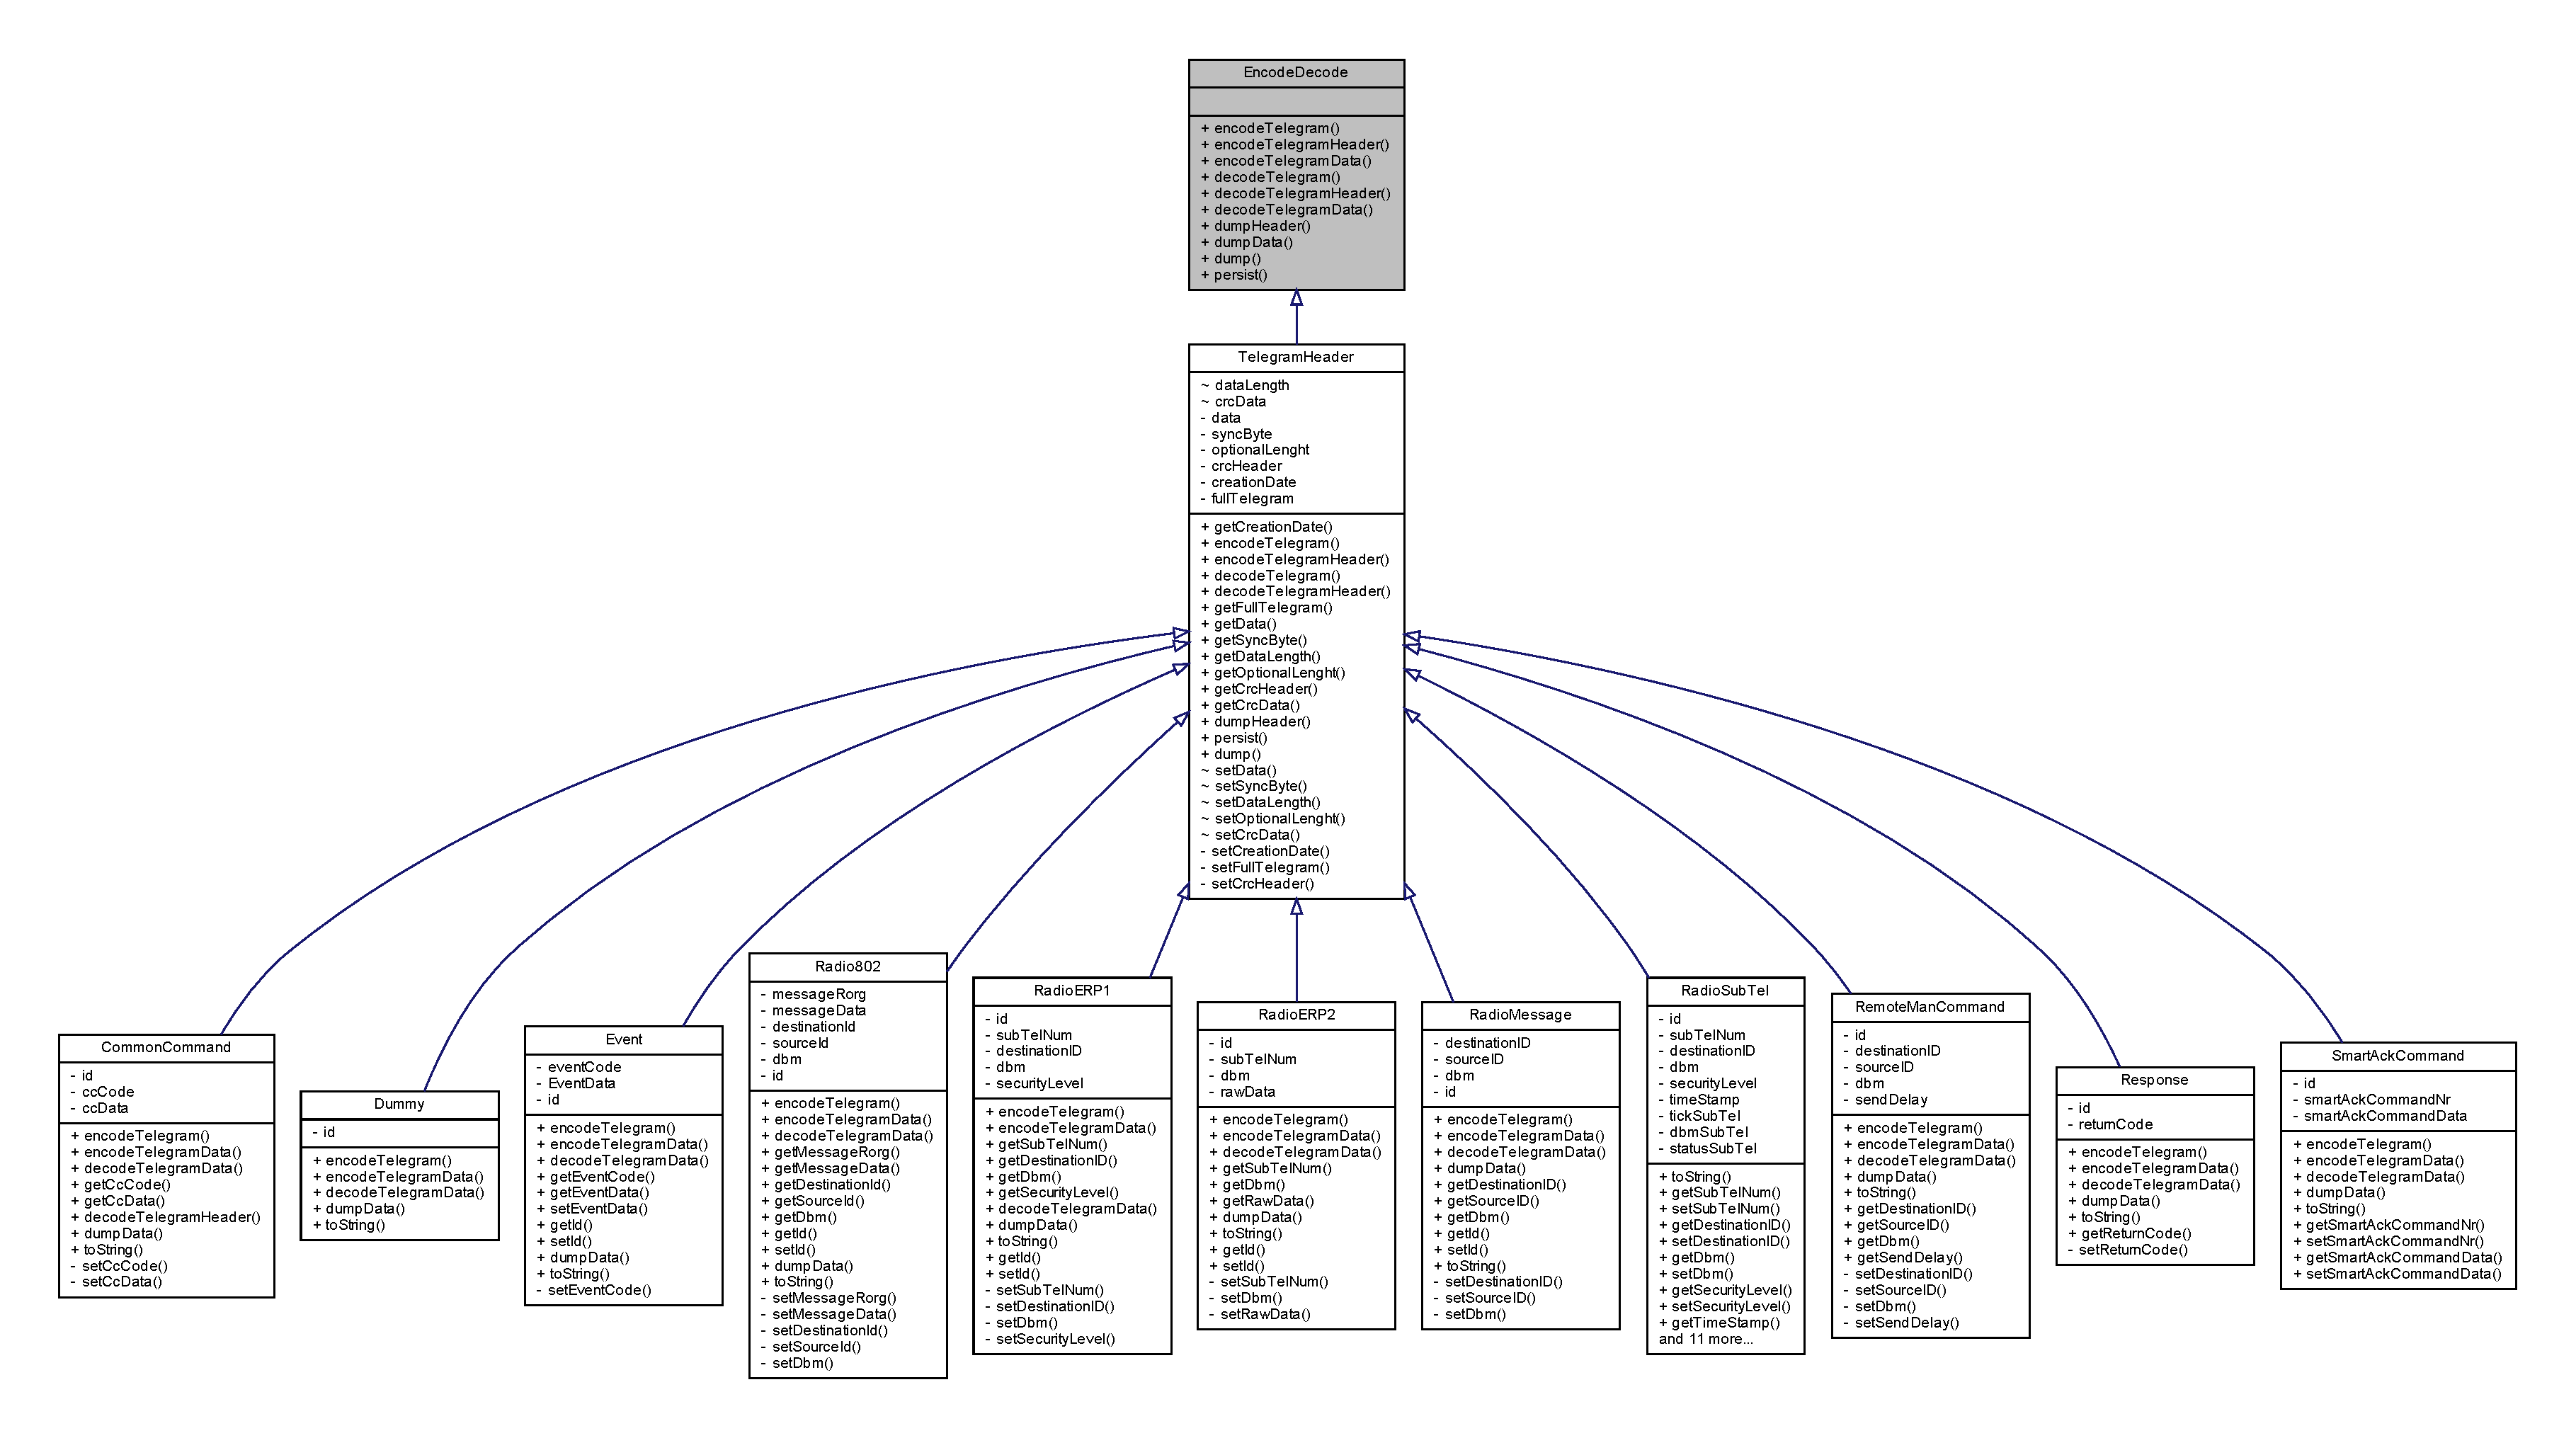
\includegraphics[width=350pt]{dd/d04/interfacech_1_1bfh_1_1gr33nopo55um_1_1enocean_1_1telegram_1_1EncodeDecode__inherit__graph}
\end{center}
\end{figure}


Collaboration diagram for Encode\+Decode\+:\nopagebreak
\begin{figure}[H]
\begin{center}
\leavevmode
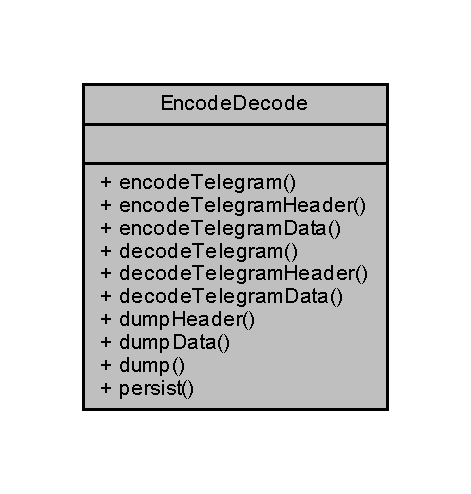
\includegraphics[width=226pt]{d8/d0b/interfacech_1_1bfh_1_1gr33nopo55um_1_1enocean_1_1telegram_1_1EncodeDecode__coll__graph}
\end{center}
\end{figure}
\subsection*{Public Member Functions}
\begin{DoxyCompactItemize}
\item 
String {\bf encode\+Telegram} ()
\begin{DoxyCompactList}\small\item\em encode\+Telegram provides an example telegram hex for this packet type. \end{DoxyCompactList}\item 
String {\bf encode\+Telegram\+Header} ()
\begin{DoxyCompactList}\small\item\em encode\+Telegram\+Header provides an example header hex for this packet type. \end{DoxyCompactList}\item 
String {\bf encode\+Telegram\+Data} ()
\begin{DoxyCompactList}\small\item\em encode\+Telegram\+Data provides an example data hex for this packet type. \end{DoxyCompactList}\item 
void {\bf decode\+Telegram} (String hex\+Telegram)
\begin{DoxyCompactList}\small\item\em decode\+Telegram splits telegram in parts \end{DoxyCompactList}\item 
void {\bf decode\+Telegram\+Header} (String hex\+Telegram)
\begin{DoxyCompactList}\small\item\em decode\+Header\+Telegram splits telegram header in parts \end{DoxyCompactList}\item 
void {\bf decode\+Telegram\+Data} (String hex\+Telegram)
\begin{DoxyCompactList}\small\item\em decode\+Telegram\+Data splits telegram data in parts \end{DoxyCompactList}\item 
void {\bf dump\+Header} ()
\begin{DoxyCompactList}\small\item\em dump\+Header Print Header, useful for logs and testing \end{DoxyCompactList}\item 
void {\bf dump\+Data} ()
\begin{DoxyCompactList}\small\item\em dump\+Data Print Data, useful for logs and testing En\+Ocean Telegram \end{DoxyCompactList}\item 
void {\bf dump} ()
\begin{DoxyCompactList}\small\item\em run both, the dump\+Header and the dump\+Data \end{DoxyCompactList}\item 
void {\bf persist} ()
\begin{DoxyCompactList}\small\item\em persist saves object to database \end{DoxyCompactList}\end{DoxyCompactItemize}


\subsection{Detailed Description}


Definition at line {\bf 7} of file {\bf Encode\+Decode.\+java}.



\subsection{Member Function Documentation}
\label{interfacech_1_1bfh_1_1gr33nopo55um_1_1enocean_1_1telegram_1_1EncodeDecode_ab5f2f0710af7330ab5f67d64983528cb} 
\index{ch\+::bfh\+::gr33nopo55um\+::enocean\+::telegram\+::\+Encode\+Decode@{ch\+::bfh\+::gr33nopo55um\+::enocean\+::telegram\+::\+Encode\+Decode}!decode\+Telegram@{decode\+Telegram}}
\index{decode\+Telegram@{decode\+Telegram}!ch\+::bfh\+::gr33nopo55um\+::enocean\+::telegram\+::\+Encode\+Decode@{ch\+::bfh\+::gr33nopo55um\+::enocean\+::telegram\+::\+Encode\+Decode}}
\subsubsection{decode\+Telegram()}
{\footnotesize\ttfamily void decode\+Telegram (\begin{DoxyParamCaption}\item[{String}]{hex\+Telegram }\end{DoxyParamCaption})}



decode\+Telegram splits telegram in parts 


\begin{DoxyParams}{Parameters}
{\em hex\+Telegram} & En\+Ocean Telegram \\
\hline
\end{DoxyParams}


Implemented in {\bf Telegram\+Header} \doxyref{}{p.}{d2/d3d/classch_1_1bfh_1_1gr33nopo55um_1_1enocean_1_1telegram_1_1TelegramHeader_ab5f2f0710af7330ab5f67d64983528cb}.

\label{interfacech_1_1bfh_1_1gr33nopo55um_1_1enocean_1_1telegram_1_1EncodeDecode_aa581cac5c3efd3142ffa8482079031e9} 
\index{ch\+::bfh\+::gr33nopo55um\+::enocean\+::telegram\+::\+Encode\+Decode@{ch\+::bfh\+::gr33nopo55um\+::enocean\+::telegram\+::\+Encode\+Decode}!decode\+Telegram\+Data@{decode\+Telegram\+Data}}
\index{decode\+Telegram\+Data@{decode\+Telegram\+Data}!ch\+::bfh\+::gr33nopo55um\+::enocean\+::telegram\+::\+Encode\+Decode@{ch\+::bfh\+::gr33nopo55um\+::enocean\+::telegram\+::\+Encode\+Decode}}
\subsubsection{decode\+Telegram\+Data()}
{\footnotesize\ttfamily void decode\+Telegram\+Data (\begin{DoxyParamCaption}\item[{String}]{hex\+Telegram }\end{DoxyParamCaption})}



decode\+Telegram\+Data splits telegram data in parts 


\begin{DoxyParams}{Parameters}
{\em hex\+Telegram} & En\+Ocean Telegram \\
\hline
\end{DoxyParams}


Implemented in {\bf Radio\+Sub\+Tel} \doxyref{}{p.}{d7/d08/classch_1_1bfh_1_1gr33nopo55um_1_1enocean_1_1telegram_1_1RadioSubTel_aa581cac5c3efd3142ffa8482079031e9}, {\bf Radio\+E\+R\+P1} \doxyref{}{p.}{d0/d7e/classch_1_1bfh_1_1gr33nopo55um_1_1enocean_1_1telegram_1_1RadioERP1_aa581cac5c3efd3142ffa8482079031e9}, {\bf Radio\+E\+R\+P2} \doxyref{}{p.}{d6/d05/classch_1_1bfh_1_1gr33nopo55um_1_1enocean_1_1telegram_1_1RadioERP2_aa581cac5c3efd3142ffa8482079031e9}, {\bf Radio802} \doxyref{}{p.}{da/d16/classch_1_1bfh_1_1gr33nopo55um_1_1enocean_1_1telegram_1_1Radio802_aa581cac5c3efd3142ffa8482079031e9}, {\bf Response} \doxyref{}{p.}{d9/dd5/classch_1_1bfh_1_1gr33nopo55um_1_1enocean_1_1telegram_1_1Response_aa581cac5c3efd3142ffa8482079031e9}, {\bf Radio\+Message} \doxyref{}{p.}{d5/dbf/classch_1_1bfh_1_1gr33nopo55um_1_1enocean_1_1telegram_1_1RadioMessage_aa581cac5c3efd3142ffa8482079031e9}, {\bf Remote\+Man\+Command} \doxyref{}{p.}{da/d94/classch_1_1bfh_1_1gr33nopo55um_1_1enocean_1_1telegram_1_1RemoteManCommand_aa581cac5c3efd3142ffa8482079031e9}, {\bf Event} \doxyref{}{p.}{d6/d3e/classch_1_1bfh_1_1gr33nopo55um_1_1enocean_1_1telegram_1_1Event_aa581cac5c3efd3142ffa8482079031e9}, {\bf Smart\+Ack\+Command} \doxyref{}{p.}{d1/dd3/classch_1_1bfh_1_1gr33nopo55um_1_1enocean_1_1telegram_1_1SmartAckCommand_aa581cac5c3efd3142ffa8482079031e9}, {\bf Common\+Command} \doxyref{}{p.}{d6/d3b/classch_1_1bfh_1_1gr33nopo55um_1_1enocean_1_1telegram_1_1CommonCommand_aa581cac5c3efd3142ffa8482079031e9}, and {\bf Dummy} \doxyref{}{p.}{d1/df6/classch_1_1bfh_1_1gr33nopo55um_1_1enocean_1_1telegram_1_1Dummy_aa581cac5c3efd3142ffa8482079031e9}.

Here is the caller graph for this function\+:\nopagebreak
\begin{figure}[H]
\begin{center}
\leavevmode
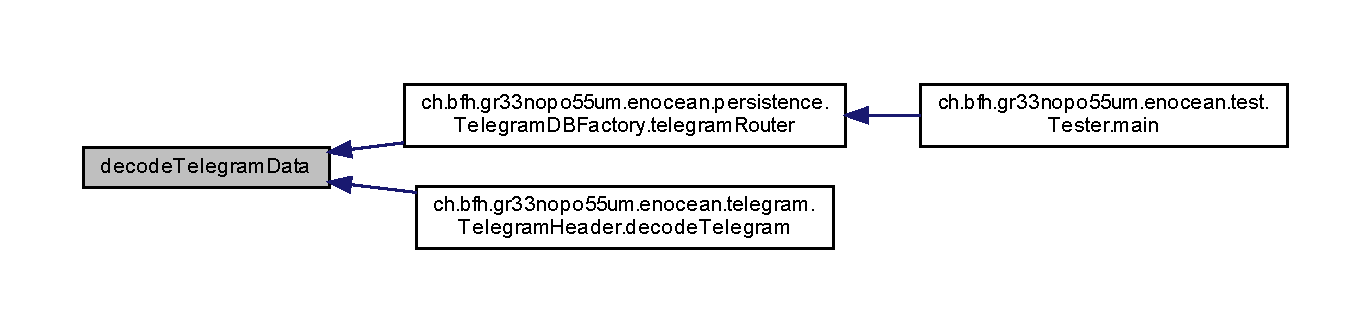
\includegraphics[width=350pt]{d1/d8c/interfacech_1_1bfh_1_1gr33nopo55um_1_1enocean_1_1telegram_1_1EncodeDecode_aa581cac5c3efd3142ffa8482079031e9_icgraph}
\end{center}
\end{figure}
\label{interfacech_1_1bfh_1_1gr33nopo55um_1_1enocean_1_1telegram_1_1EncodeDecode_a5e4622b1b692320953715a4f2dc064aa} 
\index{ch\+::bfh\+::gr33nopo55um\+::enocean\+::telegram\+::\+Encode\+Decode@{ch\+::bfh\+::gr33nopo55um\+::enocean\+::telegram\+::\+Encode\+Decode}!decode\+Telegram\+Header@{decode\+Telegram\+Header}}
\index{decode\+Telegram\+Header@{decode\+Telegram\+Header}!ch\+::bfh\+::gr33nopo55um\+::enocean\+::telegram\+::\+Encode\+Decode@{ch\+::bfh\+::gr33nopo55um\+::enocean\+::telegram\+::\+Encode\+Decode}}
\subsubsection{decode\+Telegram\+Header()}
{\footnotesize\ttfamily void decode\+Telegram\+Header (\begin{DoxyParamCaption}\item[{String}]{hex\+Telegram }\end{DoxyParamCaption})}



decode\+Header\+Telegram splits telegram header in parts 


\begin{DoxyParams}{Parameters}
{\em hex\+Telegram} & En\+Ocean Telegram \\
\hline
\end{DoxyParams}


Implemented in {\bf Common\+Command} \doxyref{}{p.}{d6/d3b/classch_1_1bfh_1_1gr33nopo55um_1_1enocean_1_1telegram_1_1CommonCommand_a5e4622b1b692320953715a4f2dc064aa}, and {\bf Telegram\+Header} \doxyref{}{p.}{d2/d3d/classch_1_1bfh_1_1gr33nopo55um_1_1enocean_1_1telegram_1_1TelegramHeader_a5e4622b1b692320953715a4f2dc064aa}.

\label{interfacech_1_1bfh_1_1gr33nopo55um_1_1enocean_1_1telegram_1_1EncodeDecode_accd2600060dbaee3a3b41aed4034c63c} 
\index{ch\+::bfh\+::gr33nopo55um\+::enocean\+::telegram\+::\+Encode\+Decode@{ch\+::bfh\+::gr33nopo55um\+::enocean\+::telegram\+::\+Encode\+Decode}!dump@{dump}}
\index{dump@{dump}!ch\+::bfh\+::gr33nopo55um\+::enocean\+::telegram\+::\+Encode\+Decode@{ch\+::bfh\+::gr33nopo55um\+::enocean\+::telegram\+::\+Encode\+Decode}}
\subsubsection{dump()}
{\footnotesize\ttfamily void dump (\begin{DoxyParamCaption}{ }\end{DoxyParamCaption})}



run both, the dump\+Header and the dump\+Data 



Implemented in {\bf Telegram\+Header} \doxyref{}{p.}{d2/d3d/classch_1_1bfh_1_1gr33nopo55um_1_1enocean_1_1telegram_1_1TelegramHeader_accd2600060dbaee3a3b41aed4034c63c}.

\label{interfacech_1_1bfh_1_1gr33nopo55um_1_1enocean_1_1telegram_1_1EncodeDecode_aff152c0c0c3d5e7011bfff0b9c08032b} 
\index{ch\+::bfh\+::gr33nopo55um\+::enocean\+::telegram\+::\+Encode\+Decode@{ch\+::bfh\+::gr33nopo55um\+::enocean\+::telegram\+::\+Encode\+Decode}!dump\+Data@{dump\+Data}}
\index{dump\+Data@{dump\+Data}!ch\+::bfh\+::gr33nopo55um\+::enocean\+::telegram\+::\+Encode\+Decode@{ch\+::bfh\+::gr33nopo55um\+::enocean\+::telegram\+::\+Encode\+Decode}}
\subsubsection{dump\+Data()}
{\footnotesize\ttfamily void dump\+Data (\begin{DoxyParamCaption}{ }\end{DoxyParamCaption})}



dump\+Data Print Data, useful for logs and testing En\+Ocean Telegram 



Implemented in {\bf Radio\+Sub\+Tel} \doxyref{}{p.}{d7/d08/classch_1_1bfh_1_1gr33nopo55um_1_1enocean_1_1telegram_1_1RadioSubTel_aff152c0c0c3d5e7011bfff0b9c08032b}, {\bf Radio802} \doxyref{}{p.}{da/d16/classch_1_1bfh_1_1gr33nopo55um_1_1enocean_1_1telegram_1_1Radio802_aff152c0c0c3d5e7011bfff0b9c08032b}, {\bf Radio\+E\+R\+P1} \doxyref{}{p.}{d0/d7e/classch_1_1bfh_1_1gr33nopo55um_1_1enocean_1_1telegram_1_1RadioERP1_aff152c0c0c3d5e7011bfff0b9c08032b}, {\bf Radio\+E\+R\+P2} \doxyref{}{p.}{d6/d05/classch_1_1bfh_1_1gr33nopo55um_1_1enocean_1_1telegram_1_1RadioERP2_aff152c0c0c3d5e7011bfff0b9c08032b}, {\bf Event} \doxyref{}{p.}{d6/d3e/classch_1_1bfh_1_1gr33nopo55um_1_1enocean_1_1telegram_1_1Event_aff152c0c0c3d5e7011bfff0b9c08032b}, {\bf Common\+Command} \doxyref{}{p.}{d6/d3b/classch_1_1bfh_1_1gr33nopo55um_1_1enocean_1_1telegram_1_1CommonCommand_aff152c0c0c3d5e7011bfff0b9c08032b}, {\bf Remote\+Man\+Command} \doxyref{}{p.}{da/d94/classch_1_1bfh_1_1gr33nopo55um_1_1enocean_1_1telegram_1_1RemoteManCommand_aff152c0c0c3d5e7011bfff0b9c08032b}, {\bf Radio\+Message} \doxyref{}{p.}{d5/dbf/classch_1_1bfh_1_1gr33nopo55um_1_1enocean_1_1telegram_1_1RadioMessage_aff152c0c0c3d5e7011bfff0b9c08032b}, {\bf Response} \doxyref{}{p.}{d9/dd5/classch_1_1bfh_1_1gr33nopo55um_1_1enocean_1_1telegram_1_1Response_aff152c0c0c3d5e7011bfff0b9c08032b}, {\bf Smart\+Ack\+Command} \doxyref{}{p.}{d1/dd3/classch_1_1bfh_1_1gr33nopo55um_1_1enocean_1_1telegram_1_1SmartAckCommand_aff152c0c0c3d5e7011bfff0b9c08032b}, and {\bf Dummy} \doxyref{}{p.}{d1/df6/classch_1_1bfh_1_1gr33nopo55um_1_1enocean_1_1telegram_1_1Dummy_aff152c0c0c3d5e7011bfff0b9c08032b}.

Here is the caller graph for this function\+:\nopagebreak
\begin{figure}[H]
\begin{center}
\leavevmode
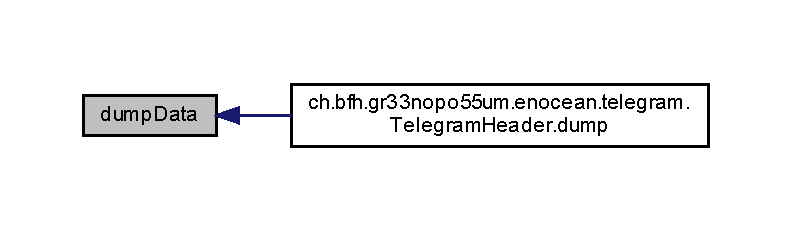
\includegraphics[width=350pt]{d1/d8c/interfacech_1_1bfh_1_1gr33nopo55um_1_1enocean_1_1telegram_1_1EncodeDecode_aff152c0c0c3d5e7011bfff0b9c08032b_icgraph}
\end{center}
\end{figure}
\label{interfacech_1_1bfh_1_1gr33nopo55um_1_1enocean_1_1telegram_1_1EncodeDecode_af74dcc31853ed58e41323c6a6f51ebf0} 
\index{ch\+::bfh\+::gr33nopo55um\+::enocean\+::telegram\+::\+Encode\+Decode@{ch\+::bfh\+::gr33nopo55um\+::enocean\+::telegram\+::\+Encode\+Decode}!dump\+Header@{dump\+Header}}
\index{dump\+Header@{dump\+Header}!ch\+::bfh\+::gr33nopo55um\+::enocean\+::telegram\+::\+Encode\+Decode@{ch\+::bfh\+::gr33nopo55um\+::enocean\+::telegram\+::\+Encode\+Decode}}
\subsubsection{dump\+Header()}
{\footnotesize\ttfamily void dump\+Header (\begin{DoxyParamCaption}{ }\end{DoxyParamCaption})}



dump\+Header Print Header, useful for logs and testing 



Implemented in {\bf Telegram\+Header} \doxyref{}{p.}{d2/d3d/classch_1_1bfh_1_1gr33nopo55um_1_1enocean_1_1telegram_1_1TelegramHeader_af74dcc31853ed58e41323c6a6f51ebf0}.

\label{interfacech_1_1bfh_1_1gr33nopo55um_1_1enocean_1_1telegram_1_1EncodeDecode_a00e3ee3b777334ef3bd46bd4105f9603} 
\index{ch\+::bfh\+::gr33nopo55um\+::enocean\+::telegram\+::\+Encode\+Decode@{ch\+::bfh\+::gr33nopo55um\+::enocean\+::telegram\+::\+Encode\+Decode}!encode\+Telegram@{encode\+Telegram}}
\index{encode\+Telegram@{encode\+Telegram}!ch\+::bfh\+::gr33nopo55um\+::enocean\+::telegram\+::\+Encode\+Decode@{ch\+::bfh\+::gr33nopo55um\+::enocean\+::telegram\+::\+Encode\+Decode}}
\subsubsection{encode\+Telegram()}
{\footnotesize\ttfamily String encode\+Telegram (\begin{DoxyParamCaption}{ }\end{DoxyParamCaption})}



encode\+Telegram provides an example telegram hex for this packet type. 

\begin{DoxyReturn}{Returns}
String hex\+Telegram En\+Ocean Telegram 
\end{DoxyReturn}


Implemented in {\bf Radio\+Sub\+Tel} \doxyref{}{p.}{d7/d08/classch_1_1bfh_1_1gr33nopo55um_1_1enocean_1_1telegram_1_1RadioSubTel_a00e3ee3b777334ef3bd46bd4105f9603}, {\bf Telegram\+Header} \doxyref{}{p.}{d2/d3d/classch_1_1bfh_1_1gr33nopo55um_1_1enocean_1_1telegram_1_1TelegramHeader_a00e3ee3b777334ef3bd46bd4105f9603}, {\bf Radio\+E\+R\+P2} \doxyref{}{p.}{d6/d05/classch_1_1bfh_1_1gr33nopo55um_1_1enocean_1_1telegram_1_1RadioERP2_a00e3ee3b777334ef3bd46bd4105f9603}, {\bf Radio802} \doxyref{}{p.}{da/d16/classch_1_1bfh_1_1gr33nopo55um_1_1enocean_1_1telegram_1_1Radio802_a00e3ee3b777334ef3bd46bd4105f9603}, {\bf Radio\+E\+R\+P1} \doxyref{}{p.}{d0/d7e/classch_1_1bfh_1_1gr33nopo55um_1_1enocean_1_1telegram_1_1RadioERP1_a00e3ee3b777334ef3bd46bd4105f9603}, {\bf Remote\+Man\+Command} \doxyref{}{p.}{da/d94/classch_1_1bfh_1_1gr33nopo55um_1_1enocean_1_1telegram_1_1RemoteManCommand_a00e3ee3b777334ef3bd46bd4105f9603}, {\bf Response} \doxyref{}{p.}{d9/dd5/classch_1_1bfh_1_1gr33nopo55um_1_1enocean_1_1telegram_1_1Response_a00e3ee3b777334ef3bd46bd4105f9603}, {\bf Radio\+Message} \doxyref{}{p.}{d5/dbf/classch_1_1bfh_1_1gr33nopo55um_1_1enocean_1_1telegram_1_1RadioMessage_a00e3ee3b777334ef3bd46bd4105f9603}, {\bf Event} \doxyref{}{p.}{d6/d3e/classch_1_1bfh_1_1gr33nopo55um_1_1enocean_1_1telegram_1_1Event_a00e3ee3b777334ef3bd46bd4105f9603}, {\bf Smart\+Ack\+Command} \doxyref{}{p.}{d1/dd3/classch_1_1bfh_1_1gr33nopo55um_1_1enocean_1_1telegram_1_1SmartAckCommand_a00e3ee3b777334ef3bd46bd4105f9603}, {\bf Common\+Command} \doxyref{}{p.}{d6/d3b/classch_1_1bfh_1_1gr33nopo55um_1_1enocean_1_1telegram_1_1CommonCommand_a00e3ee3b777334ef3bd46bd4105f9603}, and {\bf Dummy} \doxyref{}{p.}{d1/df6/classch_1_1bfh_1_1gr33nopo55um_1_1enocean_1_1telegram_1_1Dummy_a00e3ee3b777334ef3bd46bd4105f9603}.

\label{interfacech_1_1bfh_1_1gr33nopo55um_1_1enocean_1_1telegram_1_1EncodeDecode_a8a67618ab0362f3d0b60bba6ca93d883} 
\index{ch\+::bfh\+::gr33nopo55um\+::enocean\+::telegram\+::\+Encode\+Decode@{ch\+::bfh\+::gr33nopo55um\+::enocean\+::telegram\+::\+Encode\+Decode}!encode\+Telegram\+Data@{encode\+Telegram\+Data}}
\index{encode\+Telegram\+Data@{encode\+Telegram\+Data}!ch\+::bfh\+::gr33nopo55um\+::enocean\+::telegram\+::\+Encode\+Decode@{ch\+::bfh\+::gr33nopo55um\+::enocean\+::telegram\+::\+Encode\+Decode}}
\subsubsection{encode\+Telegram\+Data()}
{\footnotesize\ttfamily String encode\+Telegram\+Data (\begin{DoxyParamCaption}{ }\end{DoxyParamCaption})}



encode\+Telegram\+Data provides an example data hex for this packet type. 

\begin{DoxyReturn}{Returns}
String hex\+Telegram\+Data En\+Ocean Telegram 
\end{DoxyReturn}


Implemented in {\bf Radio\+Sub\+Tel} \doxyref{}{p.}{d7/d08/classch_1_1bfh_1_1gr33nopo55um_1_1enocean_1_1telegram_1_1RadioSubTel_a8a67618ab0362f3d0b60bba6ca93d883}, {\bf Radio\+E\+R\+P2} \doxyref{}{p.}{d6/d05/classch_1_1bfh_1_1gr33nopo55um_1_1enocean_1_1telegram_1_1RadioERP2_a8a67618ab0362f3d0b60bba6ca93d883}, {\bf Radio802} \doxyref{}{p.}{da/d16/classch_1_1bfh_1_1gr33nopo55um_1_1enocean_1_1telegram_1_1Radio802_a8a67618ab0362f3d0b60bba6ca93d883}, {\bf Radio\+E\+R\+P1} \doxyref{}{p.}{d0/d7e/classch_1_1bfh_1_1gr33nopo55um_1_1enocean_1_1telegram_1_1RadioERP1_a8a67618ab0362f3d0b60bba6ca93d883}, {\bf Response} \doxyref{}{p.}{d9/dd5/classch_1_1bfh_1_1gr33nopo55um_1_1enocean_1_1telegram_1_1Response_a8a67618ab0362f3d0b60bba6ca93d883}, {\bf Radio\+Message} \doxyref{}{p.}{d5/dbf/classch_1_1bfh_1_1gr33nopo55um_1_1enocean_1_1telegram_1_1RadioMessage_a8a67618ab0362f3d0b60bba6ca93d883}, {\bf Remote\+Man\+Command} \doxyref{}{p.}{da/d94/classch_1_1bfh_1_1gr33nopo55um_1_1enocean_1_1telegram_1_1RemoteManCommand_a8a67618ab0362f3d0b60bba6ca93d883}, {\bf Event} \doxyref{}{p.}{d6/d3e/classch_1_1bfh_1_1gr33nopo55um_1_1enocean_1_1telegram_1_1Event_a8a67618ab0362f3d0b60bba6ca93d883}, {\bf Smart\+Ack\+Command} \doxyref{}{p.}{d1/dd3/classch_1_1bfh_1_1gr33nopo55um_1_1enocean_1_1telegram_1_1SmartAckCommand_a8a67618ab0362f3d0b60bba6ca93d883}, {\bf Common\+Command} \doxyref{}{p.}{d6/d3b/classch_1_1bfh_1_1gr33nopo55um_1_1enocean_1_1telegram_1_1CommonCommand_a8a67618ab0362f3d0b60bba6ca93d883}, and {\bf Dummy} \doxyref{}{p.}{d1/df6/classch_1_1bfh_1_1gr33nopo55um_1_1enocean_1_1telegram_1_1Dummy_a8a67618ab0362f3d0b60bba6ca93d883}.

Here is the caller graph for this function\+:\nopagebreak
\begin{figure}[H]
\begin{center}
\leavevmode
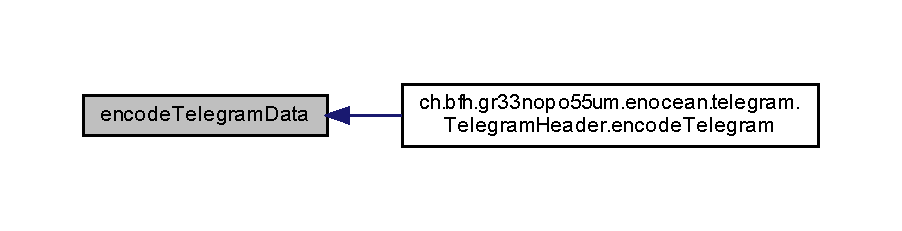
\includegraphics[width=350pt]{d1/d8c/interfacech_1_1bfh_1_1gr33nopo55um_1_1enocean_1_1telegram_1_1EncodeDecode_a8a67618ab0362f3d0b60bba6ca93d883_icgraph}
\end{center}
\end{figure}
\label{interfacech_1_1bfh_1_1gr33nopo55um_1_1enocean_1_1telegram_1_1EncodeDecode_a83697e9f527af0a6d017df13ee5e8ad7} 
\index{ch\+::bfh\+::gr33nopo55um\+::enocean\+::telegram\+::\+Encode\+Decode@{ch\+::bfh\+::gr33nopo55um\+::enocean\+::telegram\+::\+Encode\+Decode}!encode\+Telegram\+Header@{encode\+Telegram\+Header}}
\index{encode\+Telegram\+Header@{encode\+Telegram\+Header}!ch\+::bfh\+::gr33nopo55um\+::enocean\+::telegram\+::\+Encode\+Decode@{ch\+::bfh\+::gr33nopo55um\+::enocean\+::telegram\+::\+Encode\+Decode}}
\subsubsection{encode\+Telegram\+Header()}
{\footnotesize\ttfamily String encode\+Telegram\+Header (\begin{DoxyParamCaption}{ }\end{DoxyParamCaption})}



encode\+Telegram\+Header provides an example header hex for this packet type. 

\begin{DoxyReturn}{Returns}
String hex\+Telegram\+Header En\+Ocean Telegram 
\end{DoxyReturn}


Implemented in {\bf Telegram\+Header} \doxyref{}{p.}{d2/d3d/classch_1_1bfh_1_1gr33nopo55um_1_1enocean_1_1telegram_1_1TelegramHeader_a83697e9f527af0a6d017df13ee5e8ad7}.

\label{interfacech_1_1bfh_1_1gr33nopo55um_1_1enocean_1_1telegram_1_1EncodeDecode_a0551c1ea33ccc5de1fe8a6b2745d7adf} 
\index{ch\+::bfh\+::gr33nopo55um\+::enocean\+::telegram\+::\+Encode\+Decode@{ch\+::bfh\+::gr33nopo55um\+::enocean\+::telegram\+::\+Encode\+Decode}!persist@{persist}}
\index{persist@{persist}!ch\+::bfh\+::gr33nopo55um\+::enocean\+::telegram\+::\+Encode\+Decode@{ch\+::bfh\+::gr33nopo55um\+::enocean\+::telegram\+::\+Encode\+Decode}}
\subsubsection{persist()}
{\footnotesize\ttfamily void persist (\begin{DoxyParamCaption}{ }\end{DoxyParamCaption})}



persist saves object to database 



Implemented in {\bf Telegram\+Header} \doxyref{}{p.}{d2/d3d/classch_1_1bfh_1_1gr33nopo55um_1_1enocean_1_1telegram_1_1TelegramHeader_a0551c1ea33ccc5de1fe8a6b2745d7adf}.



The documentation for this interface was generated from the following file\+:\begin{DoxyCompactItemize}
\item 
/home/silas/\+Idea\+Projects/\+En\+Ocean/src/ch/bfh/gr33nopo55um/enocean/telegram/{\bf Encode\+Decode.\+java}\end{DoxyCompactItemize}

\section{Enocea\+Listener}
\label{classch_1_1bfh_1_1gr33nopo55um_1_1enocean_1_1application_1_1EnoceaListener}\index{Enocea\+Listener@{Enocea\+Listener}}


Collaboration diagram for Enocea\+Listener\+:\nopagebreak
\begin{figure}[H]
\begin{center}
\leavevmode
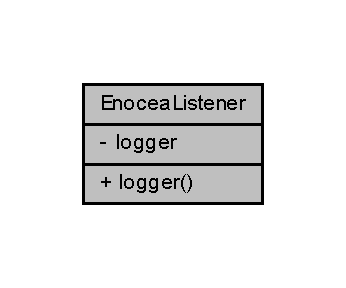
\includegraphics[width=166pt]{dc/d46/classch_1_1bfh_1_1gr33nopo55um_1_1enocean_1_1application_1_1EnoceaListener__coll__graph}
\end{center}
\end{figure}
\subsection*{Public Member Functions}
\begin{DoxyCompactItemize}
\item 
void {\bf logger} ()
\begin{DoxyCompactList}\small\item\em Logger for Serial port. \end{DoxyCompactList}\end{DoxyCompactItemize}
\subsection*{Static Private Attributes}
\begin{DoxyCompactItemize}
\item 
static Logger {\bf logger} = Log\+Manager.\+get\+Logger()
\end{DoxyCompactItemize}


\subsection{Detailed Description}


Definition at line {\bf 16} of file {\bf Enocea\+Listener.\+java}.



\subsection{Member Function Documentation}
\label{classch_1_1bfh_1_1gr33nopo55um_1_1enocean_1_1application_1_1EnoceaListener_a32382986c6aaa8ed1c7a70108a040ad8} 
\index{ch\+::bfh\+::gr33nopo55um\+::enocean\+::application\+::\+Enocea\+Listener@{ch\+::bfh\+::gr33nopo55um\+::enocean\+::application\+::\+Enocea\+Listener}!logger@{logger}}
\index{logger@{logger}!ch\+::bfh\+::gr33nopo55um\+::enocean\+::application\+::\+Enocea\+Listener@{ch\+::bfh\+::gr33nopo55um\+::enocean\+::application\+::\+Enocea\+Listener}}
\subsubsection{logger()}
{\footnotesize\ttfamily void logger (\begin{DoxyParamCaption}{ }\end{DoxyParamCaption})}



Logger for Serial port. 



Definition at line {\bf 24} of file {\bf Enocea\+Listener.\+java}.

Here is the call graph for this function\+:\nopagebreak
\begin{figure}[H]
\begin{center}
\leavevmode
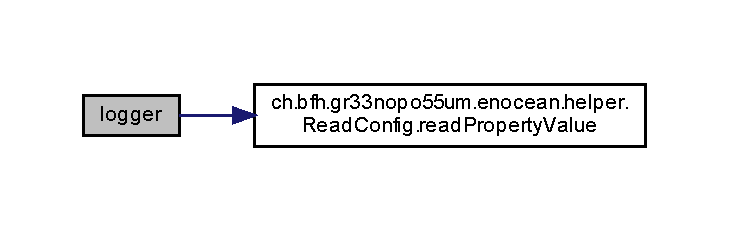
\includegraphics[width=350pt]{d5/df7/classch_1_1bfh_1_1gr33nopo55um_1_1enocean_1_1application_1_1EnoceaListener_a32382986c6aaa8ed1c7a70108a040ad8_cgraph}
\end{center}
\end{figure}


\subsection{Member Data Documentation}
\label{classch_1_1bfh_1_1gr33nopo55um_1_1enocean_1_1application_1_1EnoceaListener_a5b27630dbcf231bfda3a7d79e1eefce5} 
\index{ch\+::bfh\+::gr33nopo55um\+::enocean\+::application\+::\+Enocea\+Listener@{ch\+::bfh\+::gr33nopo55um\+::enocean\+::application\+::\+Enocea\+Listener}!logger@{logger}}
\index{logger@{logger}!ch\+::bfh\+::gr33nopo55um\+::enocean\+::application\+::\+Enocea\+Listener@{ch\+::bfh\+::gr33nopo55um\+::enocean\+::application\+::\+Enocea\+Listener}}
\subsubsection{logger}
{\footnotesize\ttfamily Logger logger = Log\+Manager.\+get\+Logger()\hspace{0.3cm}{\ttfamily [static]}, {\ttfamily [private]}}



Definition at line {\bf 18} of file {\bf Enocea\+Listener.\+java}.



The documentation for this class was generated from the following file\+:\begin{DoxyCompactItemize}
\item 
/home/silas/\+Idea\+Projects/\+En\+Ocean/src/ch/bfh/gr33nopo55um/enocean/application/{\bf Enocea\+Listener.\+java}\end{DoxyCompactItemize}

\section{E\+R\+P1}
\label{classERP1}\index{E\+R\+P1@{E\+R\+P1}}


Collaboration diagram for E\+R\+P1\+:\nopagebreak
\begin{figure}[H]
\begin{center}
\leavevmode
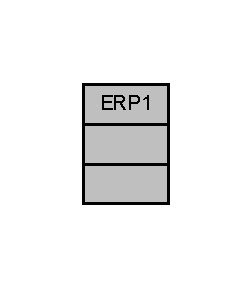
\includegraphics[width=121pt]{d5/d7b/classERP1__coll__graph}
\end{center}
\end{figure}


\subsection{Detailed Description}
\begin{DoxyAuthor}{Author}
silas , for further informations check Enocean\+Serial\+Protocol v3. \doxyref{This}{p.}{dc/d6b/classThis} is usually the default telegram type. 
\end{DoxyAuthor}


The documentation for this class was generated from the following file\+:\begin{DoxyCompactItemize}
\item 
/home/silas/\+Idea\+Projects/\+En\+Ocean/src/ch/bfh/gr33nopo55um/enocean/telegram/{\bf Radio\+E\+R\+P1.\+java}\end{DoxyCompactItemize}

\section{E\+R\+P2}
\label{classERP2}\index{E\+R\+P2@{E\+R\+P2}}


Collaboration diagram for E\+R\+P2\+:\nopagebreak
\begin{figure}[H]
\begin{center}
\leavevmode
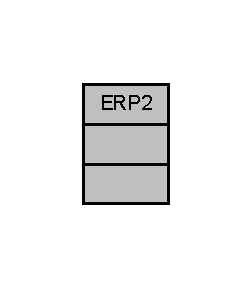
\includegraphics[width=121pt]{d3/d6c/classERP2__coll__graph}
\end{center}
\end{figure}


\subsection{Detailed Description}
telegram, for further informations check Enocean\+Serial\+Protocol v3

\begin{DoxyAuthor}{Author}
silas \& louis 
\end{DoxyAuthor}


The documentation for this class was generated from the following file\+:\begin{DoxyCompactItemize}
\item 
/home/silas/\+Idea\+Projects/\+En\+Ocean/src/ch/bfh/gr33nopo55um/enocean/telegram/{\bf Radio\+E\+R\+P2.\+java}\end{DoxyCompactItemize}

\section{Event}
\label{classch_1_1bfh_1_1gr33nopo55um_1_1enocean_1_1telegram_1_1Event}\index{Event@{Event}}


Inheritance diagram for Event\+:\nopagebreak
\begin{figure}[H]
\begin{center}
\leavevmode
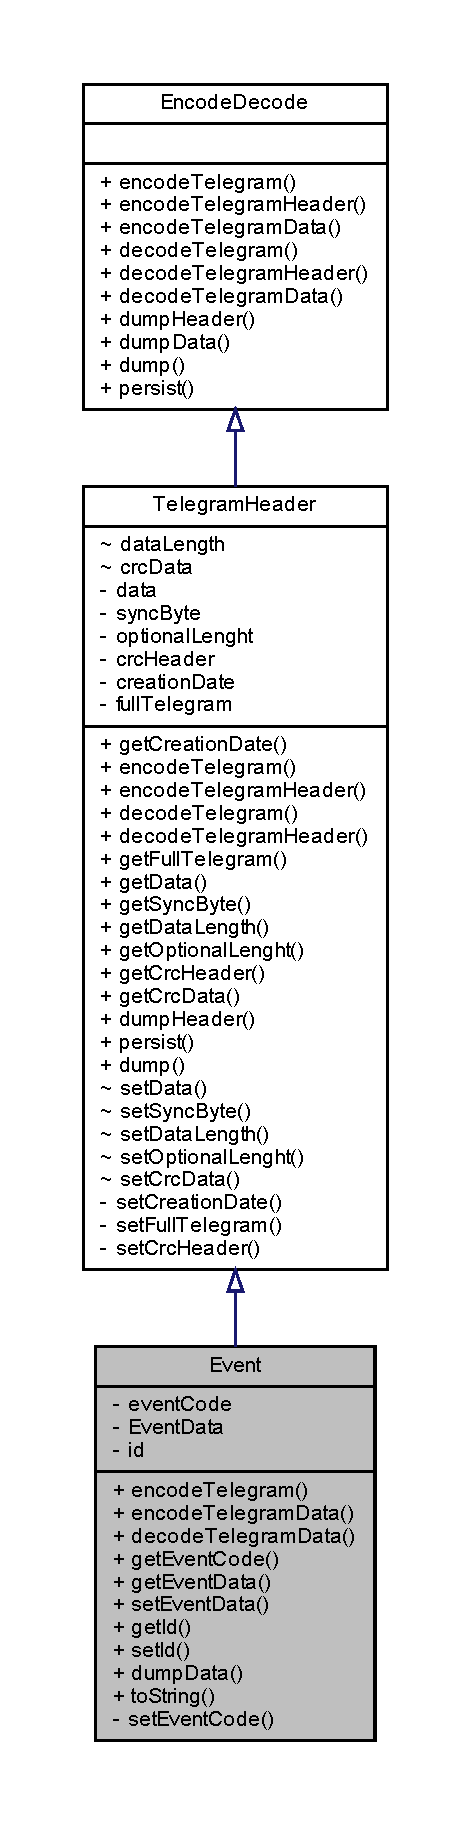
\includegraphics[height=550pt]{da/d9b/classch_1_1bfh_1_1gr33nopo55um_1_1enocean_1_1telegram_1_1Event__inherit__graph}
\end{center}
\end{figure}


Collaboration diagram for Event\+:\nopagebreak
\begin{figure}[H]
\begin{center}
\leavevmode
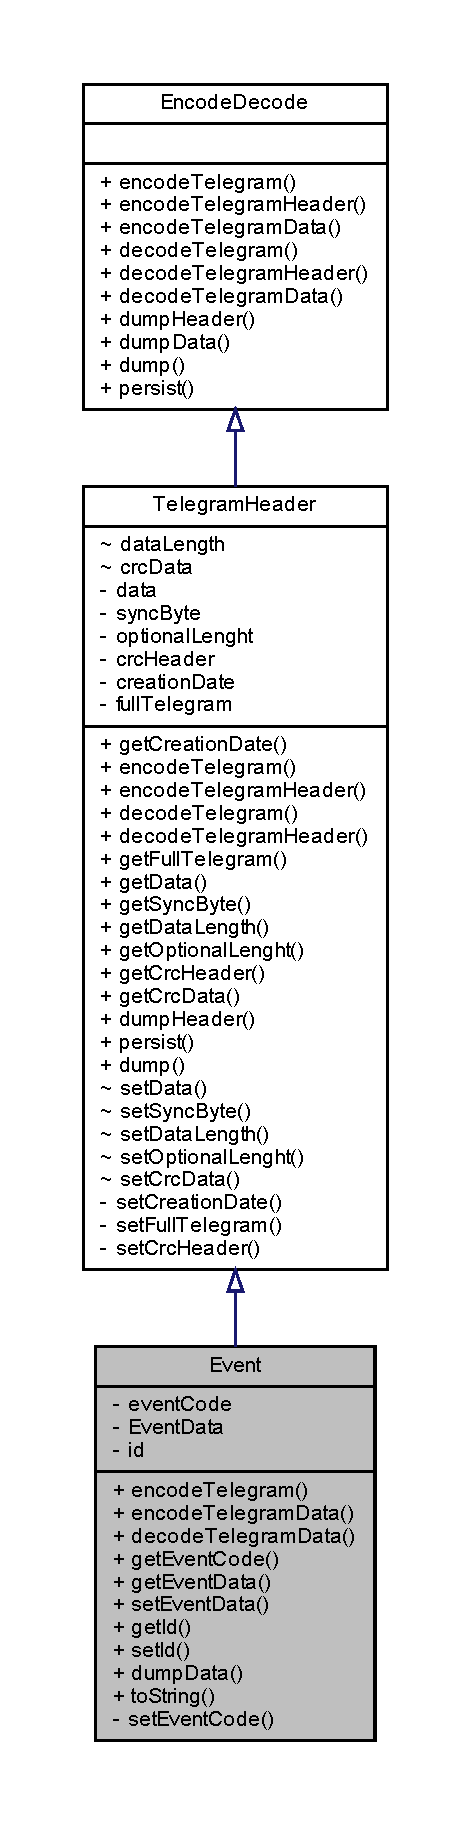
\includegraphics[height=550pt]{d1/d7a/classch_1_1bfh_1_1gr33nopo55um_1_1enocean_1_1telegram_1_1Event__coll__graph}
\end{center}
\end{figure}
\subsection*{Public Member Functions}
\begin{DoxyCompactItemize}
\item 
String {\bf encode\+Telegram} ()
\begin{DoxyCompactList}\small\item\em encode\+Telegram provides an example telegram hex for this packet type. \end{DoxyCompactList}\item 
String {\bf encode\+Telegram\+Data} ()
\begin{DoxyCompactList}\small\item\em encode\+Telegram\+Data provides an example data hex for this packet type. \end{DoxyCompactList}\item 
void {\bf decode\+Telegram\+Data} (String hex\+Telegram)
\begin{DoxyCompactList}\small\item\em decode\+Telegram\+Data splits telegram in parts \end{DoxyCompactList}\item 
int {\bf get\+Event\+Code} ()
\item 
int {\bf get\+Event\+Data} ()
\item 
void {\bf set\+Event\+Data} (int event\+Data)
\item 
Long {\bf get\+Id} ()
\item 
void {\bf set\+Id} (Long {\bf id})
\item 
void {\bf dump\+Data} ()
\begin{DoxyCompactList}\small\item\em dump\+Data Print Data, useful for logs and testing \end{DoxyCompactList}\item 
String {\bf to\+String} ()
\end{DoxyCompactItemize}
\subsection*{Private Member Functions}
\begin{DoxyCompactItemize}
\item 
void {\bf set\+Event\+Code} (int {\bf event\+Code})
\end{DoxyCompactItemize}
\subsection*{Private Attributes}
\begin{DoxyCompactItemize}
\item 
int {\bf event\+Code}
\item 
int {\bf Event\+Data}
\item 
Long {\bf id}
\end{DoxyCompactItemize}
\subsection*{Additional Inherited Members}


\subsection{Detailed Description}


Definition at line {\bf 13} of file {\bf Event.\+java}.



\subsection{Member Function Documentation}
\label{classch_1_1bfh_1_1gr33nopo55um_1_1enocean_1_1telegram_1_1Event_aa581cac5c3efd3142ffa8482079031e9} 
\index{ch\+::bfh\+::gr33nopo55um\+::enocean\+::telegram\+::\+Event@{ch\+::bfh\+::gr33nopo55um\+::enocean\+::telegram\+::\+Event}!decode\+Telegram\+Data@{decode\+Telegram\+Data}}
\index{decode\+Telegram\+Data@{decode\+Telegram\+Data}!ch\+::bfh\+::gr33nopo55um\+::enocean\+::telegram\+::\+Event@{ch\+::bfh\+::gr33nopo55um\+::enocean\+::telegram\+::\+Event}}
\subsubsection{decode\+Telegram\+Data()}
{\footnotesize\ttfamily void decode\+Telegram\+Data (\begin{DoxyParamCaption}\item[{String}]{hex\+Telegram }\end{DoxyParamCaption})}



decode\+Telegram\+Data splits telegram in parts 


\begin{DoxyParams}{Parameters}
{\em hex\+Telegram} & in hex String \\
\hline
\end{DoxyParams}


Implements {\bf Encode\+Decode} \doxyref{}{p.}{d1/d8c/interfacech_1_1bfh_1_1gr33nopo55um_1_1enocean_1_1telegram_1_1EncodeDecode_aa581cac5c3efd3142ffa8482079031e9}.



Definition at line {\bf 46} of file {\bf Event.\+java}.

Here is the call graph for this function\+:\nopagebreak
\begin{figure}[H]
\begin{center}
\leavevmode
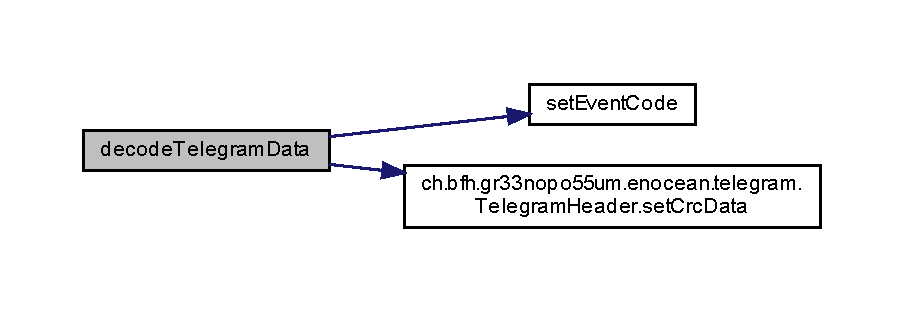
\includegraphics[width=350pt]{d6/d3e/classch_1_1bfh_1_1gr33nopo55um_1_1enocean_1_1telegram_1_1Event_aa581cac5c3efd3142ffa8482079031e9_cgraph}
\end{center}
\end{figure}
\label{classch_1_1bfh_1_1gr33nopo55um_1_1enocean_1_1telegram_1_1Event_aff152c0c0c3d5e7011bfff0b9c08032b} 
\index{ch\+::bfh\+::gr33nopo55um\+::enocean\+::telegram\+::\+Event@{ch\+::bfh\+::gr33nopo55um\+::enocean\+::telegram\+::\+Event}!dump\+Data@{dump\+Data}}
\index{dump\+Data@{dump\+Data}!ch\+::bfh\+::gr33nopo55um\+::enocean\+::telegram\+::\+Event@{ch\+::bfh\+::gr33nopo55um\+::enocean\+::telegram\+::\+Event}}
\subsubsection{dump\+Data()}
{\footnotesize\ttfamily void dump\+Data (\begin{DoxyParamCaption}{ }\end{DoxyParamCaption})}



dump\+Data Print Data, useful for logs and testing 



Implements {\bf Encode\+Decode} \doxyref{}{p.}{d1/d8c/interfacech_1_1bfh_1_1gr33nopo55um_1_1enocean_1_1telegram_1_1EncodeDecode_aff152c0c0c3d5e7011bfff0b9c08032b}.



Definition at line {\bf 83} of file {\bf Event.\+java}.

Here is the call graph for this function\+:\nopagebreak
\begin{figure}[H]
\begin{center}
\leavevmode
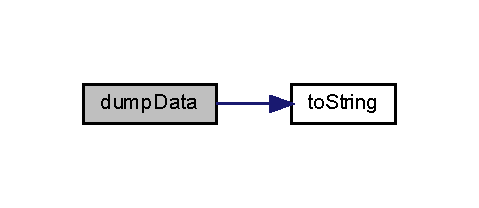
\includegraphics[width=230pt]{d6/d3e/classch_1_1bfh_1_1gr33nopo55um_1_1enocean_1_1telegram_1_1Event_aff152c0c0c3d5e7011bfff0b9c08032b_cgraph}
\end{center}
\end{figure}
\label{classch_1_1bfh_1_1gr33nopo55um_1_1enocean_1_1telegram_1_1Event_a00e3ee3b777334ef3bd46bd4105f9603} 
\index{ch\+::bfh\+::gr33nopo55um\+::enocean\+::telegram\+::\+Event@{ch\+::bfh\+::gr33nopo55um\+::enocean\+::telegram\+::\+Event}!encode\+Telegram@{encode\+Telegram}}
\index{encode\+Telegram@{encode\+Telegram}!ch\+::bfh\+::gr33nopo55um\+::enocean\+::telegram\+::\+Event@{ch\+::bfh\+::gr33nopo55um\+::enocean\+::telegram\+::\+Event}}
\subsubsection{encode\+Telegram()}
{\footnotesize\ttfamily String encode\+Telegram (\begin{DoxyParamCaption}{ }\end{DoxyParamCaption})}



encode\+Telegram provides an example telegram hex for this packet type. 

\begin{DoxyReturn}{Returns}
telegram hex 
\end{DoxyReturn}


Implements {\bf Encode\+Decode} \doxyref{}{p.}{d1/d8c/interfacech_1_1bfh_1_1gr33nopo55um_1_1enocean_1_1telegram_1_1EncodeDecode_a00e3ee3b777334ef3bd46bd4105f9603}.



Definition at line {\bf 28} of file {\bf Event.\+java}.

\label{classch_1_1bfh_1_1gr33nopo55um_1_1enocean_1_1telegram_1_1Event_a8a67618ab0362f3d0b60bba6ca93d883} 
\index{ch\+::bfh\+::gr33nopo55um\+::enocean\+::telegram\+::\+Event@{ch\+::bfh\+::gr33nopo55um\+::enocean\+::telegram\+::\+Event}!encode\+Telegram\+Data@{encode\+Telegram\+Data}}
\index{encode\+Telegram\+Data@{encode\+Telegram\+Data}!ch\+::bfh\+::gr33nopo55um\+::enocean\+::telegram\+::\+Event@{ch\+::bfh\+::gr33nopo55um\+::enocean\+::telegram\+::\+Event}}
\subsubsection{encode\+Telegram\+Data()}
{\footnotesize\ttfamily String encode\+Telegram\+Data (\begin{DoxyParamCaption}{ }\end{DoxyParamCaption})}



encode\+Telegram\+Data provides an example data hex for this packet type. 

\begin{DoxyReturn}{Returns}
String hex\+Telegram\+Data En\+Ocean Telegram 
\end{DoxyReturn}


Implements {\bf Encode\+Decode} \doxyref{}{p.}{d1/d8c/interfacech_1_1bfh_1_1gr33nopo55um_1_1enocean_1_1telegram_1_1EncodeDecode_a8a67618ab0362f3d0b60bba6ca93d883}.



Definition at line {\bf 37} of file {\bf Event.\+java}.

\label{classch_1_1bfh_1_1gr33nopo55um_1_1enocean_1_1telegram_1_1Event_a6b37ae2c9337aca6629d93844088da01} 
\index{ch\+::bfh\+::gr33nopo55um\+::enocean\+::telegram\+::\+Event@{ch\+::bfh\+::gr33nopo55um\+::enocean\+::telegram\+::\+Event}!get\+Event\+Code@{get\+Event\+Code}}
\index{get\+Event\+Code@{get\+Event\+Code}!ch\+::bfh\+::gr33nopo55um\+::enocean\+::telegram\+::\+Event@{ch\+::bfh\+::gr33nopo55um\+::enocean\+::telegram\+::\+Event}}
\subsubsection{get\+Event\+Code()}
{\footnotesize\ttfamily int get\+Event\+Code (\begin{DoxyParamCaption}{ }\end{DoxyParamCaption})}



Definition at line {\bf 55} of file {\bf Event.\+java}.

\label{classch_1_1bfh_1_1gr33nopo55um_1_1enocean_1_1telegram_1_1Event_a62e121db952facd008bf374d9bd05e33} 
\index{ch\+::bfh\+::gr33nopo55um\+::enocean\+::telegram\+::\+Event@{ch\+::bfh\+::gr33nopo55um\+::enocean\+::telegram\+::\+Event}!get\+Event\+Data@{get\+Event\+Data}}
\index{get\+Event\+Data@{get\+Event\+Data}!ch\+::bfh\+::gr33nopo55um\+::enocean\+::telegram\+::\+Event@{ch\+::bfh\+::gr33nopo55um\+::enocean\+::telegram\+::\+Event}}
\subsubsection{get\+Event\+Data()}
{\footnotesize\ttfamily int get\+Event\+Data (\begin{DoxyParamCaption}{ }\end{DoxyParamCaption})}



Definition at line {\bf 63} of file {\bf Event.\+java}.

\label{classch_1_1bfh_1_1gr33nopo55um_1_1enocean_1_1telegram_1_1Event_a30e533a51833664ad05441781ee6a6a0} 
\index{ch\+::bfh\+::gr33nopo55um\+::enocean\+::telegram\+::\+Event@{ch\+::bfh\+::gr33nopo55um\+::enocean\+::telegram\+::\+Event}!get\+Id@{get\+Id}}
\index{get\+Id@{get\+Id}!ch\+::bfh\+::gr33nopo55um\+::enocean\+::telegram\+::\+Event@{ch\+::bfh\+::gr33nopo55um\+::enocean\+::telegram\+::\+Event}}
\subsubsection{get\+Id()}
{\footnotesize\ttfamily Long get\+Id (\begin{DoxyParamCaption}{ }\end{DoxyParamCaption})}



Definition at line {\bf 71} of file {\bf Event.\+java}.

\label{classch_1_1bfh_1_1gr33nopo55um_1_1enocean_1_1telegram_1_1Event_a3e244ad20c9d10874f3a26a5da310cca} 
\index{ch\+::bfh\+::gr33nopo55um\+::enocean\+::telegram\+::\+Event@{ch\+::bfh\+::gr33nopo55um\+::enocean\+::telegram\+::\+Event}!set\+Event\+Code@{set\+Event\+Code}}
\index{set\+Event\+Code@{set\+Event\+Code}!ch\+::bfh\+::gr33nopo55um\+::enocean\+::telegram\+::\+Event@{ch\+::bfh\+::gr33nopo55um\+::enocean\+::telegram\+::\+Event}}
\subsubsection{set\+Event\+Code()}
{\footnotesize\ttfamily void set\+Event\+Code (\begin{DoxyParamCaption}\item[{int}]{event\+Code }\end{DoxyParamCaption})\hspace{0.3cm}{\ttfamily [private]}}



Definition at line {\bf 59} of file {\bf Event.\+java}.

Here is the caller graph for this function\+:\nopagebreak
\begin{figure}[H]
\begin{center}
\leavevmode
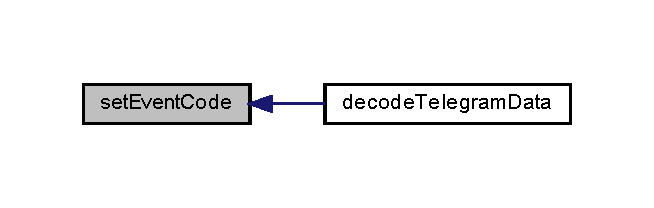
\includegraphics[width=314pt]{d6/d3e/classch_1_1bfh_1_1gr33nopo55um_1_1enocean_1_1telegram_1_1Event_a3e244ad20c9d10874f3a26a5da310cca_icgraph}
\end{center}
\end{figure}
\label{classch_1_1bfh_1_1gr33nopo55um_1_1enocean_1_1telegram_1_1Event_a39087ae2feb3f48754e6099afd83cdfa} 
\index{ch\+::bfh\+::gr33nopo55um\+::enocean\+::telegram\+::\+Event@{ch\+::bfh\+::gr33nopo55um\+::enocean\+::telegram\+::\+Event}!set\+Event\+Data@{set\+Event\+Data}}
\index{set\+Event\+Data@{set\+Event\+Data}!ch\+::bfh\+::gr33nopo55um\+::enocean\+::telegram\+::\+Event@{ch\+::bfh\+::gr33nopo55um\+::enocean\+::telegram\+::\+Event}}
\subsubsection{set\+Event\+Data()}
{\footnotesize\ttfamily void set\+Event\+Data (\begin{DoxyParamCaption}\item[{int}]{event\+Data }\end{DoxyParamCaption})}



Definition at line {\bf 67} of file {\bf Event.\+java}.

\label{classch_1_1bfh_1_1gr33nopo55um_1_1enocean_1_1telegram_1_1Event_ae855b9b14d52c956a065d1a71f74a136} 
\index{ch\+::bfh\+::gr33nopo55um\+::enocean\+::telegram\+::\+Event@{ch\+::bfh\+::gr33nopo55um\+::enocean\+::telegram\+::\+Event}!set\+Id@{set\+Id}}
\index{set\+Id@{set\+Id}!ch\+::bfh\+::gr33nopo55um\+::enocean\+::telegram\+::\+Event@{ch\+::bfh\+::gr33nopo55um\+::enocean\+::telegram\+::\+Event}}
\subsubsection{set\+Id()}
{\footnotesize\ttfamily void set\+Id (\begin{DoxyParamCaption}\item[{Long}]{id }\end{DoxyParamCaption})}



Definition at line {\bf 75} of file {\bf Event.\+java}.

\label{classch_1_1bfh_1_1gr33nopo55um_1_1enocean_1_1telegram_1_1Event_ad146fa8579a5f8a876c4688cc5a68520} 
\index{ch\+::bfh\+::gr33nopo55um\+::enocean\+::telegram\+::\+Event@{ch\+::bfh\+::gr33nopo55um\+::enocean\+::telegram\+::\+Event}!to\+String@{to\+String}}
\index{to\+String@{to\+String}!ch\+::bfh\+::gr33nopo55um\+::enocean\+::telegram\+::\+Event@{ch\+::bfh\+::gr33nopo55um\+::enocean\+::telegram\+::\+Event}}
\subsubsection{to\+String()}
{\footnotesize\ttfamily String to\+String (\begin{DoxyParamCaption}{ }\end{DoxyParamCaption})}



Definition at line {\bf 89} of file {\bf Event.\+java}.

Here is the caller graph for this function\+:\nopagebreak
\begin{figure}[H]
\begin{center}
\leavevmode
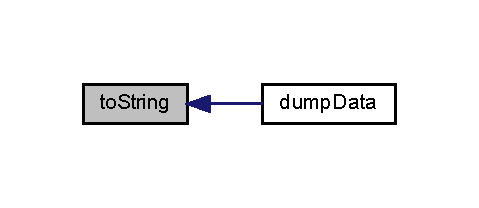
\includegraphics[width=230pt]{d6/d3e/classch_1_1bfh_1_1gr33nopo55um_1_1enocean_1_1telegram_1_1Event_ad146fa8579a5f8a876c4688cc5a68520_icgraph}
\end{center}
\end{figure}


\subsection{Member Data Documentation}
\label{classch_1_1bfh_1_1gr33nopo55um_1_1enocean_1_1telegram_1_1Event_a678f143cd7557ea790f1eaea0bcc0c0d} 
\index{ch\+::bfh\+::gr33nopo55um\+::enocean\+::telegram\+::\+Event@{ch\+::bfh\+::gr33nopo55um\+::enocean\+::telegram\+::\+Event}!event\+Code@{event\+Code}}
\index{event\+Code@{event\+Code}!ch\+::bfh\+::gr33nopo55um\+::enocean\+::telegram\+::\+Event@{ch\+::bfh\+::gr33nopo55um\+::enocean\+::telegram\+::\+Event}}
\subsubsection{event\+Code}
{\footnotesize\ttfamily int event\+Code\hspace{0.3cm}{\ttfamily [private]}}



Definition at line {\bf 15} of file {\bf Event.\+java}.

\label{classch_1_1bfh_1_1gr33nopo55um_1_1enocean_1_1telegram_1_1Event_a1dfd9af56f648714e935e6a4d3e0f7f6} 
\index{ch\+::bfh\+::gr33nopo55um\+::enocean\+::telegram\+::\+Event@{ch\+::bfh\+::gr33nopo55um\+::enocean\+::telegram\+::\+Event}!Event\+Data@{Event\+Data}}
\index{Event\+Data@{Event\+Data}!ch\+::bfh\+::gr33nopo55um\+::enocean\+::telegram\+::\+Event@{ch\+::bfh\+::gr33nopo55um\+::enocean\+::telegram\+::\+Event}}
\subsubsection{Event\+Data}
{\footnotesize\ttfamily int Event\+Data\hspace{0.3cm}{\ttfamily [private]}}



Definition at line {\bf 16} of file {\bf Event.\+java}.

\label{classch_1_1bfh_1_1gr33nopo55um_1_1enocean_1_1telegram_1_1Event_afdea3f4ac85ac5819c978584be2be48e} 
\index{ch\+::bfh\+::gr33nopo55um\+::enocean\+::telegram\+::\+Event@{ch\+::bfh\+::gr33nopo55um\+::enocean\+::telegram\+::\+Event}!id@{id}}
\index{id@{id}!ch\+::bfh\+::gr33nopo55um\+::enocean\+::telegram\+::\+Event@{ch\+::bfh\+::gr33nopo55um\+::enocean\+::telegram\+::\+Event}}
\subsubsection{id}
{\footnotesize\ttfamily Long id\hspace{0.3cm}{\ttfamily [private]}}



Definition at line {\bf 20} of file {\bf Event.\+java}.



The documentation for this class was generated from the following file\+:\begin{DoxyCompactItemize}
\item 
/home/silas/\+Idea\+Projects/\+En\+Ocean/src/ch/bfh/gr33nopo55um/enocean/telegram/{\bf Event.\+java}\end{DoxyCompactItemize}

\section{Logic}
\label{classLogic}\index{Logic@{Logic}}


Collaboration diagram for Logic\+:\nopagebreak
\begin{figure}[H]
\begin{center}
\leavevmode
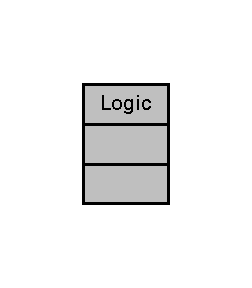
\includegraphics[width=121pt]{d2/d6b/classLogic__coll__graph}
\end{center}
\end{figure}


\subsection{Detailed Description}
\begin{DoxyAuthor}{Author}
silas which packettype should be persisted. 
\end{DoxyAuthor}


The documentation for this class was generated from the following file\+:\begin{DoxyCompactItemize}
\item 
/home/silas/\+Idea\+Projects/\+En\+Ocean/src/ch/bfh/gr33nopo55um/enocean/persistence/{\bf Telegram\+D\+B\+Factory.\+java}\end{DoxyCompactItemize}

\section{Main}
\label{classMain}\index{Main@{Main}}


Collaboration diagram for Main\+:\nopagebreak
\begin{figure}[H]
\begin{center}
\leavevmode
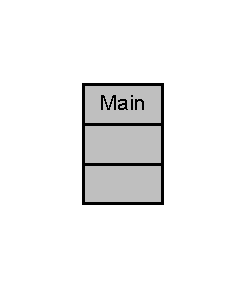
\includegraphics[width=118pt]{d7/d2c/classMain__coll__graph}
\end{center}
\end{figure}


\subsection{Detailed Description}
\begin{DoxyAuthor}{Author}
silas 
\end{DoxyAuthor}


The documentation for this class was generated from the following file\+:\begin{DoxyCompactItemize}
\item 
/home/silas/\+Idea\+Projects/\+En\+Ocean/src/ch/bfh/gr33nopo55um/enocean/application/{\bf Application.\+java}\end{DoxyCompactItemize}

\section{Physical}
\label{classPhysical}\index{Physical@{Physical}}


Collaboration diagram for Physical\+:\nopagebreak
\begin{figure}[H]
\begin{center}
\leavevmode
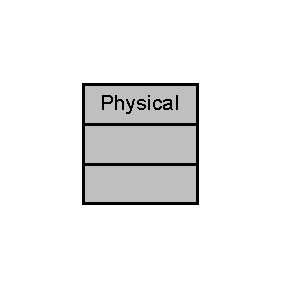
\includegraphics[width=135pt]{d9/d7c/classPhysical__coll__graph}
\end{center}
\end{figure}


\subsection{Detailed Description}
\begin{DoxyAuthor}{Author}
silas \& louis , for further informations check Enocean\+Serial\+Protocol v3 
\end{DoxyAuthor}


The documentation for this class was generated from the following file\+:\begin{DoxyCompactItemize}
\item 
/home/silas/\+Idea\+Projects/\+En\+Ocean/src/ch/bfh/gr33nopo55um/enocean/telegram/{\bf Radio802.\+java}\end{DoxyCompactItemize}

\section{Radio}
\label{classRadio}\index{Radio@{Radio}}


Collaboration diagram for Radio\+:\nopagebreak
\begin{figure}[H]
\begin{center}
\leavevmode
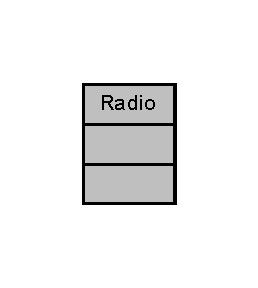
\includegraphics[width=124pt]{df/dd6/classRadio__coll__graph}
\end{center}
\end{figure}


\subsection{Detailed Description}
data without any radio telegram contents, for further informations check Enocean\+Serial\+Protocol v3

\begin{DoxyAuthor}{Author}
silas \& louis 
\end{DoxyAuthor}


The documentation for this class was generated from the following file\+:\begin{DoxyCompactItemize}
\item 
/home/silas/\+Idea\+Projects/\+En\+Ocean/src/ch/bfh/gr33nopo55um/enocean/telegram/{\bf Radio\+Message.\+java}\end{DoxyCompactItemize}

\section{Radio802}
\label{classch_1_1bfh_1_1gr33nopo55um_1_1enocean_1_1telegram_1_1Radio802}\index{Radio802@{Radio802}}


Inheritance diagram for Radio802\+:\nopagebreak
\begin{figure}[H]
\begin{center}
\leavevmode
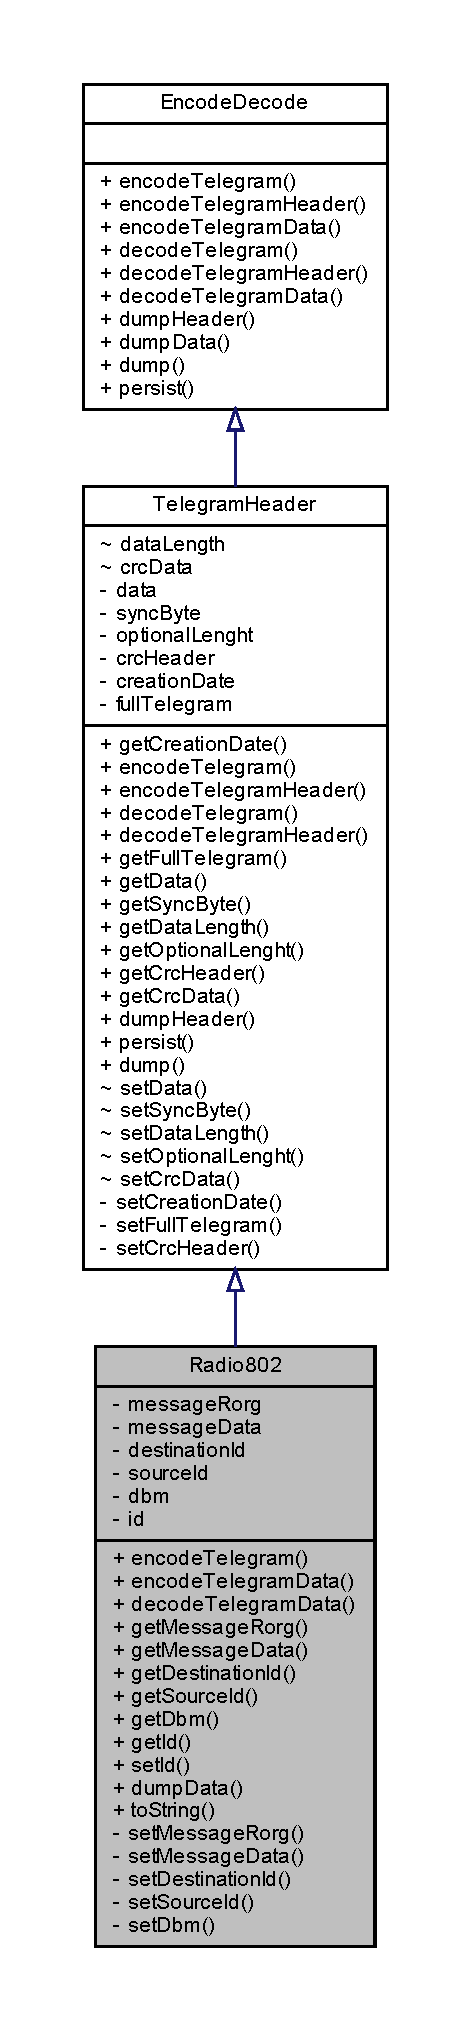
\includegraphics[height=550pt]{d1/da3/classch_1_1bfh_1_1gr33nopo55um_1_1enocean_1_1telegram_1_1Radio802__inherit__graph}
\end{center}
\end{figure}


Collaboration diagram for Radio802\+:\nopagebreak
\begin{figure}[H]
\begin{center}
\leavevmode
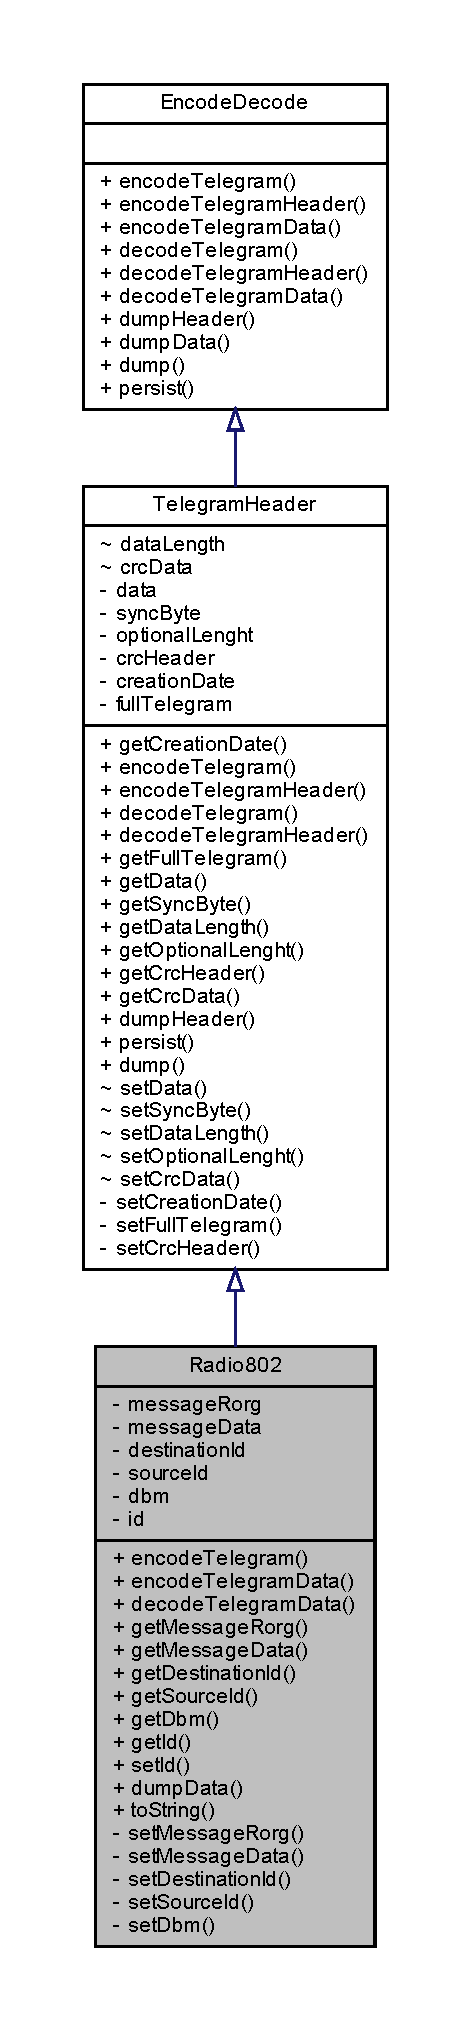
\includegraphics[height=550pt]{d1/d29/classch_1_1bfh_1_1gr33nopo55um_1_1enocean_1_1telegram_1_1Radio802__coll__graph}
\end{center}
\end{figure}
\subsection*{Public Member Functions}
\begin{DoxyCompactItemize}
\item 
String {\bf encode\+Telegram} ()
\begin{DoxyCompactList}\small\item\em encode\+Telegram provides an example telegram hex for this packet type. \end{DoxyCompactList}\item 
String {\bf encode\+Telegram\+Data} ()
\begin{DoxyCompactList}\small\item\em encode\+Telegram\+Data provides an example data hex for this packet type. \end{DoxyCompactList}\item 
void {\bf decode\+Telegram\+Data} (String hex\+Telegram)
\begin{DoxyCompactList}\small\item\em decode\+Telegram\+Data splits telegram in parts \end{DoxyCompactList}\item 
int {\bf get\+Message\+Rorg} ()
\item 
int {\bf get\+Message\+Data} ()
\item 
int {\bf get\+Destination\+Id} ()
\item 
int {\bf get\+Source\+Id} ()
\item 
int {\bf get\+Dbm} ()
\item 
Long {\bf get\+Id} ()
\item 
void {\bf set\+Id} (Long {\bf id})
\item 
void {\bf dump\+Data} ()
\begin{DoxyCompactList}\small\item\em dump\+Data Print Data, useful for logs and testiing \end{DoxyCompactList}\item 
String {\bf to\+String} ()
\end{DoxyCompactItemize}
\subsection*{Private Member Functions}
\begin{DoxyCompactItemize}
\item 
void {\bf set\+Message\+Rorg} (int {\bf message\+Rorg})
\item 
void {\bf set\+Message\+Data} (int {\bf message\+Data})
\item 
void {\bf set\+Destination\+Id} (int {\bf destination\+Id})
\item 
void {\bf set\+Source\+Id} (int {\bf source\+Id})
\item 
void {\bf set\+Dbm} (int {\bf dbm})
\end{DoxyCompactItemize}
\subsection*{Private Attributes}
\begin{DoxyCompactItemize}
\item 
int {\bf message\+Rorg}
\item 
int {\bf message\+Data}
\item 
int {\bf destination\+Id}
\item 
int {\bf source\+Id}
\item 
int {\bf dbm}
\item 
Long {\bf id}
\end{DoxyCompactItemize}
\subsection*{Additional Inherited Members}


\subsection{Detailed Description}


Definition at line {\bf 13} of file {\bf Radio802.\+java}.



\subsection{Member Function Documentation}
\label{classch_1_1bfh_1_1gr33nopo55um_1_1enocean_1_1telegram_1_1Radio802_aa581cac5c3efd3142ffa8482079031e9} 
\index{ch\+::bfh\+::gr33nopo55um\+::enocean\+::telegram\+::\+Radio802@{ch\+::bfh\+::gr33nopo55um\+::enocean\+::telegram\+::\+Radio802}!decode\+Telegram\+Data@{decode\+Telegram\+Data}}
\index{decode\+Telegram\+Data@{decode\+Telegram\+Data}!ch\+::bfh\+::gr33nopo55um\+::enocean\+::telegram\+::\+Radio802@{ch\+::bfh\+::gr33nopo55um\+::enocean\+::telegram\+::\+Radio802}}
\subsubsection{decode\+Telegram\+Data()}
{\footnotesize\ttfamily void decode\+Telegram\+Data (\begin{DoxyParamCaption}\item[{String}]{hex\+Telegram }\end{DoxyParamCaption})}



decode\+Telegram\+Data splits telegram in parts 


\begin{DoxyParams}{Parameters}
{\em hex\+Telegram} & in hex String \\
\hline
\end{DoxyParams}


Implements {\bf Encode\+Decode} \doxyref{}{p.}{d1/d8c/interfacech_1_1bfh_1_1gr33nopo55um_1_1enocean_1_1telegram_1_1EncodeDecode_aa581cac5c3efd3142ffa8482079031e9}.



Definition at line {\bf 50} of file {\bf Radio802.\+java}.

Here is the call graph for this function\+:\nopagebreak
\begin{figure}[H]
\begin{center}
\leavevmode
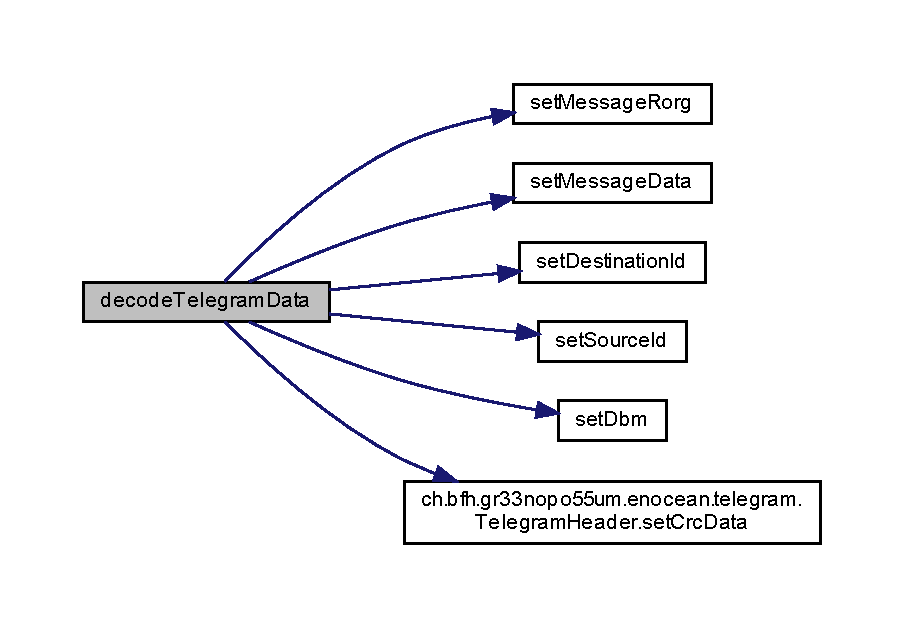
\includegraphics[width=350pt]{da/d16/classch_1_1bfh_1_1gr33nopo55um_1_1enocean_1_1telegram_1_1Radio802_aa581cac5c3efd3142ffa8482079031e9_cgraph}
\end{center}
\end{figure}
\label{classch_1_1bfh_1_1gr33nopo55um_1_1enocean_1_1telegram_1_1Radio802_aff152c0c0c3d5e7011bfff0b9c08032b} 
\index{ch\+::bfh\+::gr33nopo55um\+::enocean\+::telegram\+::\+Radio802@{ch\+::bfh\+::gr33nopo55um\+::enocean\+::telegram\+::\+Radio802}!dump\+Data@{dump\+Data}}
\index{dump\+Data@{dump\+Data}!ch\+::bfh\+::gr33nopo55um\+::enocean\+::telegram\+::\+Radio802@{ch\+::bfh\+::gr33nopo55um\+::enocean\+::telegram\+::\+Radio802}}
\subsubsection{dump\+Data()}
{\footnotesize\ttfamily void dump\+Data (\begin{DoxyParamCaption}{ }\end{DoxyParamCaption})}



dump\+Data Print Data, useful for logs and testiing 



Implements {\bf Encode\+Decode} \doxyref{}{p.}{d1/d8c/interfacech_1_1bfh_1_1gr33nopo55um_1_1enocean_1_1telegram_1_1EncodeDecode_aff152c0c0c3d5e7011bfff0b9c08032b}.



Definition at line {\bf 114} of file {\bf Radio802.\+java}.

Here is the call graph for this function\+:\nopagebreak
\begin{figure}[H]
\begin{center}
\leavevmode
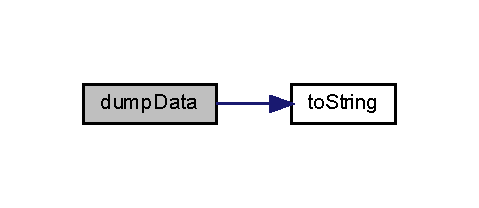
\includegraphics[width=230pt]{da/d16/classch_1_1bfh_1_1gr33nopo55um_1_1enocean_1_1telegram_1_1Radio802_aff152c0c0c3d5e7011bfff0b9c08032b_cgraph}
\end{center}
\end{figure}
\label{classch_1_1bfh_1_1gr33nopo55um_1_1enocean_1_1telegram_1_1Radio802_a00e3ee3b777334ef3bd46bd4105f9603} 
\index{ch\+::bfh\+::gr33nopo55um\+::enocean\+::telegram\+::\+Radio802@{ch\+::bfh\+::gr33nopo55um\+::enocean\+::telegram\+::\+Radio802}!encode\+Telegram@{encode\+Telegram}}
\index{encode\+Telegram@{encode\+Telegram}!ch\+::bfh\+::gr33nopo55um\+::enocean\+::telegram\+::\+Radio802@{ch\+::bfh\+::gr33nopo55um\+::enocean\+::telegram\+::\+Radio802}}
\subsubsection{encode\+Telegram()}
{\footnotesize\ttfamily String encode\+Telegram (\begin{DoxyParamCaption}{ }\end{DoxyParamCaption})}



encode\+Telegram provides an example telegram hex for this packet type. 

\begin{DoxyReturn}{Returns}
telegram hex 
\end{DoxyReturn}


Implements {\bf Encode\+Decode} \doxyref{}{p.}{d1/d8c/interfacech_1_1bfh_1_1gr33nopo55um_1_1enocean_1_1telegram_1_1EncodeDecode_a00e3ee3b777334ef3bd46bd4105f9603}.



Definition at line {\bf 32} of file {\bf Radio802.\+java}.

\label{classch_1_1bfh_1_1gr33nopo55um_1_1enocean_1_1telegram_1_1Radio802_a8a67618ab0362f3d0b60bba6ca93d883} 
\index{ch\+::bfh\+::gr33nopo55um\+::enocean\+::telegram\+::\+Radio802@{ch\+::bfh\+::gr33nopo55um\+::enocean\+::telegram\+::\+Radio802}!encode\+Telegram\+Data@{encode\+Telegram\+Data}}
\index{encode\+Telegram\+Data@{encode\+Telegram\+Data}!ch\+::bfh\+::gr33nopo55um\+::enocean\+::telegram\+::\+Radio802@{ch\+::bfh\+::gr33nopo55um\+::enocean\+::telegram\+::\+Radio802}}
\subsubsection{encode\+Telegram\+Data()}
{\footnotesize\ttfamily String encode\+Telegram\+Data (\begin{DoxyParamCaption}{ }\end{DoxyParamCaption})}



encode\+Telegram\+Data provides an example data hex for this packet type. 

\begin{DoxyReturn}{Returns}
String hex\+Telegram\+Data En\+Ocean Telegram 
\end{DoxyReturn}


Implements {\bf Encode\+Decode} \doxyref{}{p.}{d1/d8c/interfacech_1_1bfh_1_1gr33nopo55um_1_1enocean_1_1telegram_1_1EncodeDecode_a8a67618ab0362f3d0b60bba6ca93d883}.



Definition at line {\bf 41} of file {\bf Radio802.\+java}.

\label{classch_1_1bfh_1_1gr33nopo55um_1_1enocean_1_1telegram_1_1Radio802_a41fc3f0b91116ab725e007c5cea15def} 
\index{ch\+::bfh\+::gr33nopo55um\+::enocean\+::telegram\+::\+Radio802@{ch\+::bfh\+::gr33nopo55um\+::enocean\+::telegram\+::\+Radio802}!get\+Dbm@{get\+Dbm}}
\index{get\+Dbm@{get\+Dbm}!ch\+::bfh\+::gr33nopo55um\+::enocean\+::telegram\+::\+Radio802@{ch\+::bfh\+::gr33nopo55um\+::enocean\+::telegram\+::\+Radio802}}
\subsubsection{get\+Dbm()}
{\footnotesize\ttfamily int get\+Dbm (\begin{DoxyParamCaption}{ }\end{DoxyParamCaption})}



Definition at line {\bf 94} of file {\bf Radio802.\+java}.

\label{classch_1_1bfh_1_1gr33nopo55um_1_1enocean_1_1telegram_1_1Radio802_a63ddf9f15cb8e21f71cd3e03116d274c} 
\index{ch\+::bfh\+::gr33nopo55um\+::enocean\+::telegram\+::\+Radio802@{ch\+::bfh\+::gr33nopo55um\+::enocean\+::telegram\+::\+Radio802}!get\+Destination\+Id@{get\+Destination\+Id}}
\index{get\+Destination\+Id@{get\+Destination\+Id}!ch\+::bfh\+::gr33nopo55um\+::enocean\+::telegram\+::\+Radio802@{ch\+::bfh\+::gr33nopo55um\+::enocean\+::telegram\+::\+Radio802}}
\subsubsection{get\+Destination\+Id()}
{\footnotesize\ttfamily int get\+Destination\+Id (\begin{DoxyParamCaption}{ }\end{DoxyParamCaption})}



Definition at line {\bf 78} of file {\bf Radio802.\+java}.

\label{classch_1_1bfh_1_1gr33nopo55um_1_1enocean_1_1telegram_1_1Radio802_a30e533a51833664ad05441781ee6a6a0} 
\index{ch\+::bfh\+::gr33nopo55um\+::enocean\+::telegram\+::\+Radio802@{ch\+::bfh\+::gr33nopo55um\+::enocean\+::telegram\+::\+Radio802}!get\+Id@{get\+Id}}
\index{get\+Id@{get\+Id}!ch\+::bfh\+::gr33nopo55um\+::enocean\+::telegram\+::\+Radio802@{ch\+::bfh\+::gr33nopo55um\+::enocean\+::telegram\+::\+Radio802}}
\subsubsection{get\+Id()}
{\footnotesize\ttfamily Long get\+Id (\begin{DoxyParamCaption}{ }\end{DoxyParamCaption})}



Definition at line {\bf 102} of file {\bf Radio802.\+java}.

\label{classch_1_1bfh_1_1gr33nopo55um_1_1enocean_1_1telegram_1_1Radio802_ac9c914e77d35d66fce874706f807d1fb} 
\index{ch\+::bfh\+::gr33nopo55um\+::enocean\+::telegram\+::\+Radio802@{ch\+::bfh\+::gr33nopo55um\+::enocean\+::telegram\+::\+Radio802}!get\+Message\+Data@{get\+Message\+Data}}
\index{get\+Message\+Data@{get\+Message\+Data}!ch\+::bfh\+::gr33nopo55um\+::enocean\+::telegram\+::\+Radio802@{ch\+::bfh\+::gr33nopo55um\+::enocean\+::telegram\+::\+Radio802}}
\subsubsection{get\+Message\+Data()}
{\footnotesize\ttfamily int get\+Message\+Data (\begin{DoxyParamCaption}{ }\end{DoxyParamCaption})}



Definition at line {\bf 70} of file {\bf Radio802.\+java}.

\label{classch_1_1bfh_1_1gr33nopo55um_1_1enocean_1_1telegram_1_1Radio802_aedf3caf9c3c13f151372a2ad3288dfa2} 
\index{ch\+::bfh\+::gr33nopo55um\+::enocean\+::telegram\+::\+Radio802@{ch\+::bfh\+::gr33nopo55um\+::enocean\+::telegram\+::\+Radio802}!get\+Message\+Rorg@{get\+Message\+Rorg}}
\index{get\+Message\+Rorg@{get\+Message\+Rorg}!ch\+::bfh\+::gr33nopo55um\+::enocean\+::telegram\+::\+Radio802@{ch\+::bfh\+::gr33nopo55um\+::enocean\+::telegram\+::\+Radio802}}
\subsubsection{get\+Message\+Rorg()}
{\footnotesize\ttfamily int get\+Message\+Rorg (\begin{DoxyParamCaption}{ }\end{DoxyParamCaption})}



Definition at line {\bf 62} of file {\bf Radio802.\+java}.

\label{classch_1_1bfh_1_1gr33nopo55um_1_1enocean_1_1telegram_1_1Radio802_a87f8c113b178021e76e9f34256bcba7e} 
\index{ch\+::bfh\+::gr33nopo55um\+::enocean\+::telegram\+::\+Radio802@{ch\+::bfh\+::gr33nopo55um\+::enocean\+::telegram\+::\+Radio802}!get\+Source\+Id@{get\+Source\+Id}}
\index{get\+Source\+Id@{get\+Source\+Id}!ch\+::bfh\+::gr33nopo55um\+::enocean\+::telegram\+::\+Radio802@{ch\+::bfh\+::gr33nopo55um\+::enocean\+::telegram\+::\+Radio802}}
\subsubsection{get\+Source\+Id()}
{\footnotesize\ttfamily int get\+Source\+Id (\begin{DoxyParamCaption}{ }\end{DoxyParamCaption})}



Definition at line {\bf 86} of file {\bf Radio802.\+java}.

\label{classch_1_1bfh_1_1gr33nopo55um_1_1enocean_1_1telegram_1_1Radio802_a17374793c87ff1a128532736cc1bb082} 
\index{ch\+::bfh\+::gr33nopo55um\+::enocean\+::telegram\+::\+Radio802@{ch\+::bfh\+::gr33nopo55um\+::enocean\+::telegram\+::\+Radio802}!set\+Dbm@{set\+Dbm}}
\index{set\+Dbm@{set\+Dbm}!ch\+::bfh\+::gr33nopo55um\+::enocean\+::telegram\+::\+Radio802@{ch\+::bfh\+::gr33nopo55um\+::enocean\+::telegram\+::\+Radio802}}
\subsubsection{set\+Dbm()}
{\footnotesize\ttfamily void set\+Dbm (\begin{DoxyParamCaption}\item[{int}]{dbm }\end{DoxyParamCaption})\hspace{0.3cm}{\ttfamily [private]}}



Definition at line {\bf 98} of file {\bf Radio802.\+java}.

Here is the caller graph for this function\+:\nopagebreak
\begin{figure}[H]
\begin{center}
\leavevmode
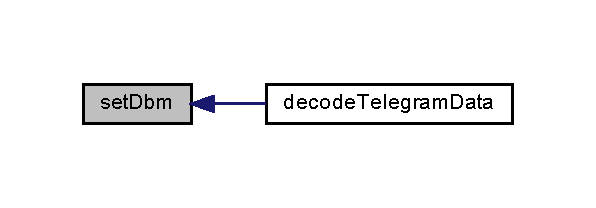
\includegraphics[width=286pt]{da/d16/classch_1_1bfh_1_1gr33nopo55um_1_1enocean_1_1telegram_1_1Radio802_a17374793c87ff1a128532736cc1bb082_icgraph}
\end{center}
\end{figure}
\label{classch_1_1bfh_1_1gr33nopo55um_1_1enocean_1_1telegram_1_1Radio802_a4bace731194d509223670a425b26649c} 
\index{ch\+::bfh\+::gr33nopo55um\+::enocean\+::telegram\+::\+Radio802@{ch\+::bfh\+::gr33nopo55um\+::enocean\+::telegram\+::\+Radio802}!set\+Destination\+Id@{set\+Destination\+Id}}
\index{set\+Destination\+Id@{set\+Destination\+Id}!ch\+::bfh\+::gr33nopo55um\+::enocean\+::telegram\+::\+Radio802@{ch\+::bfh\+::gr33nopo55um\+::enocean\+::telegram\+::\+Radio802}}
\subsubsection{set\+Destination\+Id()}
{\footnotesize\ttfamily void set\+Destination\+Id (\begin{DoxyParamCaption}\item[{int}]{destination\+Id }\end{DoxyParamCaption})\hspace{0.3cm}{\ttfamily [private]}}



Definition at line {\bf 82} of file {\bf Radio802.\+java}.

Here is the caller graph for this function\+:\nopagebreak
\begin{figure}[H]
\begin{center}
\leavevmode
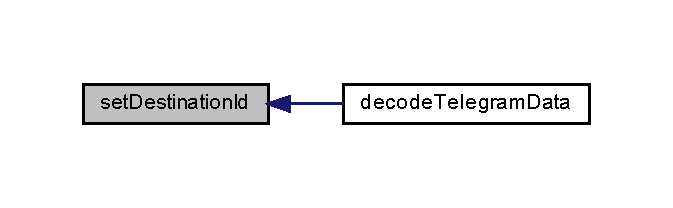
\includegraphics[width=323pt]{da/d16/classch_1_1bfh_1_1gr33nopo55um_1_1enocean_1_1telegram_1_1Radio802_a4bace731194d509223670a425b26649c_icgraph}
\end{center}
\end{figure}
\label{classch_1_1bfh_1_1gr33nopo55um_1_1enocean_1_1telegram_1_1Radio802_ae855b9b14d52c956a065d1a71f74a136} 
\index{ch\+::bfh\+::gr33nopo55um\+::enocean\+::telegram\+::\+Radio802@{ch\+::bfh\+::gr33nopo55um\+::enocean\+::telegram\+::\+Radio802}!set\+Id@{set\+Id}}
\index{set\+Id@{set\+Id}!ch\+::bfh\+::gr33nopo55um\+::enocean\+::telegram\+::\+Radio802@{ch\+::bfh\+::gr33nopo55um\+::enocean\+::telegram\+::\+Radio802}}
\subsubsection{set\+Id()}
{\footnotesize\ttfamily void set\+Id (\begin{DoxyParamCaption}\item[{Long}]{id }\end{DoxyParamCaption})}



Definition at line {\bf 106} of file {\bf Radio802.\+java}.

\label{classch_1_1bfh_1_1gr33nopo55um_1_1enocean_1_1telegram_1_1Radio802_a5792cf031e0d1bcc26b13e2fcdd0aedc} 
\index{ch\+::bfh\+::gr33nopo55um\+::enocean\+::telegram\+::\+Radio802@{ch\+::bfh\+::gr33nopo55um\+::enocean\+::telegram\+::\+Radio802}!set\+Message\+Data@{set\+Message\+Data}}
\index{set\+Message\+Data@{set\+Message\+Data}!ch\+::bfh\+::gr33nopo55um\+::enocean\+::telegram\+::\+Radio802@{ch\+::bfh\+::gr33nopo55um\+::enocean\+::telegram\+::\+Radio802}}
\subsubsection{set\+Message\+Data()}
{\footnotesize\ttfamily void set\+Message\+Data (\begin{DoxyParamCaption}\item[{int}]{message\+Data }\end{DoxyParamCaption})\hspace{0.3cm}{\ttfamily [private]}}



Definition at line {\bf 74} of file {\bf Radio802.\+java}.

Here is the caller graph for this function\+:\nopagebreak
\begin{figure}[H]
\begin{center}
\leavevmode
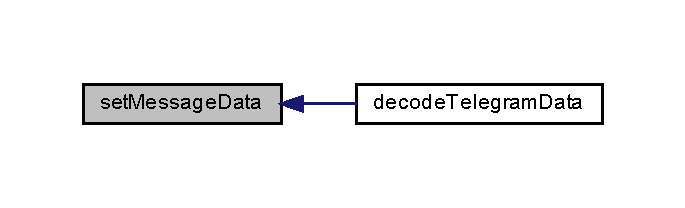
\includegraphics[width=329pt]{da/d16/classch_1_1bfh_1_1gr33nopo55um_1_1enocean_1_1telegram_1_1Radio802_a5792cf031e0d1bcc26b13e2fcdd0aedc_icgraph}
\end{center}
\end{figure}
\label{classch_1_1bfh_1_1gr33nopo55um_1_1enocean_1_1telegram_1_1Radio802_a40322aaf1ca2711dfb46776d54f6f52e} 
\index{ch\+::bfh\+::gr33nopo55um\+::enocean\+::telegram\+::\+Radio802@{ch\+::bfh\+::gr33nopo55um\+::enocean\+::telegram\+::\+Radio802}!set\+Message\+Rorg@{set\+Message\+Rorg}}
\index{set\+Message\+Rorg@{set\+Message\+Rorg}!ch\+::bfh\+::gr33nopo55um\+::enocean\+::telegram\+::\+Radio802@{ch\+::bfh\+::gr33nopo55um\+::enocean\+::telegram\+::\+Radio802}}
\subsubsection{set\+Message\+Rorg()}
{\footnotesize\ttfamily void set\+Message\+Rorg (\begin{DoxyParamCaption}\item[{int}]{message\+Rorg }\end{DoxyParamCaption})\hspace{0.3cm}{\ttfamily [private]}}



Definition at line {\bf 66} of file {\bf Radio802.\+java}.

Here is the caller graph for this function\+:\nopagebreak
\begin{figure}[H]
\begin{center}
\leavevmode
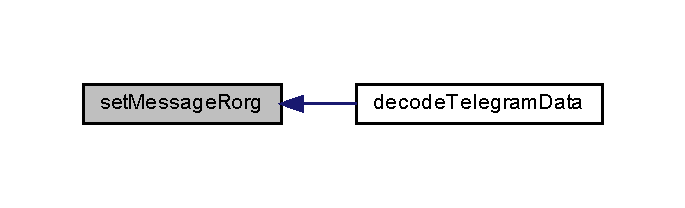
\includegraphics[width=329pt]{da/d16/classch_1_1bfh_1_1gr33nopo55um_1_1enocean_1_1telegram_1_1Radio802_a40322aaf1ca2711dfb46776d54f6f52e_icgraph}
\end{center}
\end{figure}
\label{classch_1_1bfh_1_1gr33nopo55um_1_1enocean_1_1telegram_1_1Radio802_a3b719e8e4102c3ae97b662648e3046fd} 
\index{ch\+::bfh\+::gr33nopo55um\+::enocean\+::telegram\+::\+Radio802@{ch\+::bfh\+::gr33nopo55um\+::enocean\+::telegram\+::\+Radio802}!set\+Source\+Id@{set\+Source\+Id}}
\index{set\+Source\+Id@{set\+Source\+Id}!ch\+::bfh\+::gr33nopo55um\+::enocean\+::telegram\+::\+Radio802@{ch\+::bfh\+::gr33nopo55um\+::enocean\+::telegram\+::\+Radio802}}
\subsubsection{set\+Source\+Id()}
{\footnotesize\ttfamily void set\+Source\+Id (\begin{DoxyParamCaption}\item[{int}]{source\+Id }\end{DoxyParamCaption})\hspace{0.3cm}{\ttfamily [private]}}



Definition at line {\bf 90} of file {\bf Radio802.\+java}.

Here is the caller graph for this function\+:\nopagebreak
\begin{figure}[H]
\begin{center}
\leavevmode
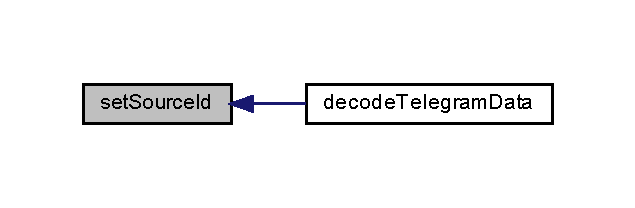
\includegraphics[width=305pt]{da/d16/classch_1_1bfh_1_1gr33nopo55um_1_1enocean_1_1telegram_1_1Radio802_a3b719e8e4102c3ae97b662648e3046fd_icgraph}
\end{center}
\end{figure}
\label{classch_1_1bfh_1_1gr33nopo55um_1_1enocean_1_1telegram_1_1Radio802_ad146fa8579a5f8a876c4688cc5a68520} 
\index{ch\+::bfh\+::gr33nopo55um\+::enocean\+::telegram\+::\+Radio802@{ch\+::bfh\+::gr33nopo55um\+::enocean\+::telegram\+::\+Radio802}!to\+String@{to\+String}}
\index{to\+String@{to\+String}!ch\+::bfh\+::gr33nopo55um\+::enocean\+::telegram\+::\+Radio802@{ch\+::bfh\+::gr33nopo55um\+::enocean\+::telegram\+::\+Radio802}}
\subsubsection{to\+String()}
{\footnotesize\ttfamily String to\+String (\begin{DoxyParamCaption}{ }\end{DoxyParamCaption})}



Definition at line {\bf 124} of file {\bf Radio802.\+java}.

Here is the caller graph for this function\+:\nopagebreak
\begin{figure}[H]
\begin{center}
\leavevmode
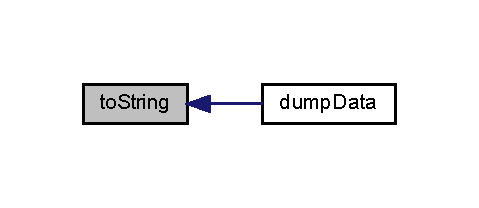
\includegraphics[width=230pt]{da/d16/classch_1_1bfh_1_1gr33nopo55um_1_1enocean_1_1telegram_1_1Radio802_ad146fa8579a5f8a876c4688cc5a68520_icgraph}
\end{center}
\end{figure}


\subsection{Member Data Documentation}
\label{classch_1_1bfh_1_1gr33nopo55um_1_1enocean_1_1telegram_1_1Radio802_ad2c3b8f9fd4bbc30208e66b69c290dc6} 
\index{ch\+::bfh\+::gr33nopo55um\+::enocean\+::telegram\+::\+Radio802@{ch\+::bfh\+::gr33nopo55um\+::enocean\+::telegram\+::\+Radio802}!dbm@{dbm}}
\index{dbm@{dbm}!ch\+::bfh\+::gr33nopo55um\+::enocean\+::telegram\+::\+Radio802@{ch\+::bfh\+::gr33nopo55um\+::enocean\+::telegram\+::\+Radio802}}
\subsubsection{dbm}
{\footnotesize\ttfamily int dbm\hspace{0.3cm}{\ttfamily [private]}}



Definition at line {\bf 21} of file {\bf Radio802.\+java}.

\label{classch_1_1bfh_1_1gr33nopo55um_1_1enocean_1_1telegram_1_1Radio802_a7945f51aeeb63b585c13a8adfc6feeb9} 
\index{ch\+::bfh\+::gr33nopo55um\+::enocean\+::telegram\+::\+Radio802@{ch\+::bfh\+::gr33nopo55um\+::enocean\+::telegram\+::\+Radio802}!destination\+Id@{destination\+Id}}
\index{destination\+Id@{destination\+Id}!ch\+::bfh\+::gr33nopo55um\+::enocean\+::telegram\+::\+Radio802@{ch\+::bfh\+::gr33nopo55um\+::enocean\+::telegram\+::\+Radio802}}
\subsubsection{destination\+Id}
{\footnotesize\ttfamily int destination\+Id\hspace{0.3cm}{\ttfamily [private]}}



Definition at line {\bf 18} of file {\bf Radio802.\+java}.

\label{classch_1_1bfh_1_1gr33nopo55um_1_1enocean_1_1telegram_1_1Radio802_afdea3f4ac85ac5819c978584be2be48e} 
\index{ch\+::bfh\+::gr33nopo55um\+::enocean\+::telegram\+::\+Radio802@{ch\+::bfh\+::gr33nopo55um\+::enocean\+::telegram\+::\+Radio802}!id@{id}}
\index{id@{id}!ch\+::bfh\+::gr33nopo55um\+::enocean\+::telegram\+::\+Radio802@{ch\+::bfh\+::gr33nopo55um\+::enocean\+::telegram\+::\+Radio802}}
\subsubsection{id}
{\footnotesize\ttfamily Long id\hspace{0.3cm}{\ttfamily [private]}}



Definition at line {\bf 24} of file {\bf Radio802.\+java}.

\label{classch_1_1bfh_1_1gr33nopo55um_1_1enocean_1_1telegram_1_1Radio802_a7a73fbb66042c771a8c03875b5167bd1} 
\index{ch\+::bfh\+::gr33nopo55um\+::enocean\+::telegram\+::\+Radio802@{ch\+::bfh\+::gr33nopo55um\+::enocean\+::telegram\+::\+Radio802}!message\+Data@{message\+Data}}
\index{message\+Data@{message\+Data}!ch\+::bfh\+::gr33nopo55um\+::enocean\+::telegram\+::\+Radio802@{ch\+::bfh\+::gr33nopo55um\+::enocean\+::telegram\+::\+Radio802}}
\subsubsection{message\+Data}
{\footnotesize\ttfamily int message\+Data\hspace{0.3cm}{\ttfamily [private]}}



Definition at line {\bf 16} of file {\bf Radio802.\+java}.

\label{classch_1_1bfh_1_1gr33nopo55um_1_1enocean_1_1telegram_1_1Radio802_a062902143a4444eb3cdbd60a8c8ec32f} 
\index{ch\+::bfh\+::gr33nopo55um\+::enocean\+::telegram\+::\+Radio802@{ch\+::bfh\+::gr33nopo55um\+::enocean\+::telegram\+::\+Radio802}!message\+Rorg@{message\+Rorg}}
\index{message\+Rorg@{message\+Rorg}!ch\+::bfh\+::gr33nopo55um\+::enocean\+::telegram\+::\+Radio802@{ch\+::bfh\+::gr33nopo55um\+::enocean\+::telegram\+::\+Radio802}}
\subsubsection{message\+Rorg}
{\footnotesize\ttfamily int message\+Rorg\hspace{0.3cm}{\ttfamily [private]}}



Definition at line {\bf 15} of file {\bf Radio802.\+java}.

\label{classch_1_1bfh_1_1gr33nopo55um_1_1enocean_1_1telegram_1_1Radio802_a10352af2f085e1be546d57ad209878f4} 
\index{ch\+::bfh\+::gr33nopo55um\+::enocean\+::telegram\+::\+Radio802@{ch\+::bfh\+::gr33nopo55um\+::enocean\+::telegram\+::\+Radio802}!source\+Id@{source\+Id}}
\index{source\+Id@{source\+Id}!ch\+::bfh\+::gr33nopo55um\+::enocean\+::telegram\+::\+Radio802@{ch\+::bfh\+::gr33nopo55um\+::enocean\+::telegram\+::\+Radio802}}
\subsubsection{source\+Id}
{\footnotesize\ttfamily int source\+Id\hspace{0.3cm}{\ttfamily [private]}}



Definition at line {\bf 20} of file {\bf Radio802.\+java}.



The documentation for this class was generated from the following file\+:\begin{DoxyCompactItemize}
\item 
/home/silas/\+Idea\+Projects/\+En\+Ocean/src/ch/bfh/gr33nopo55um/enocean/telegram/{\bf Radio802.\+java}\end{DoxyCompactItemize}

\section{Radio\+E\+R\+P1}
\label{classch_1_1bfh_1_1gr33nopo55um_1_1enocean_1_1telegram_1_1RadioERP1}\index{Radio\+E\+R\+P1@{Radio\+E\+R\+P1}}


Inheritance diagram for Radio\+E\+R\+P1\+:\nopagebreak
\begin{figure}[H]
\begin{center}
\leavevmode
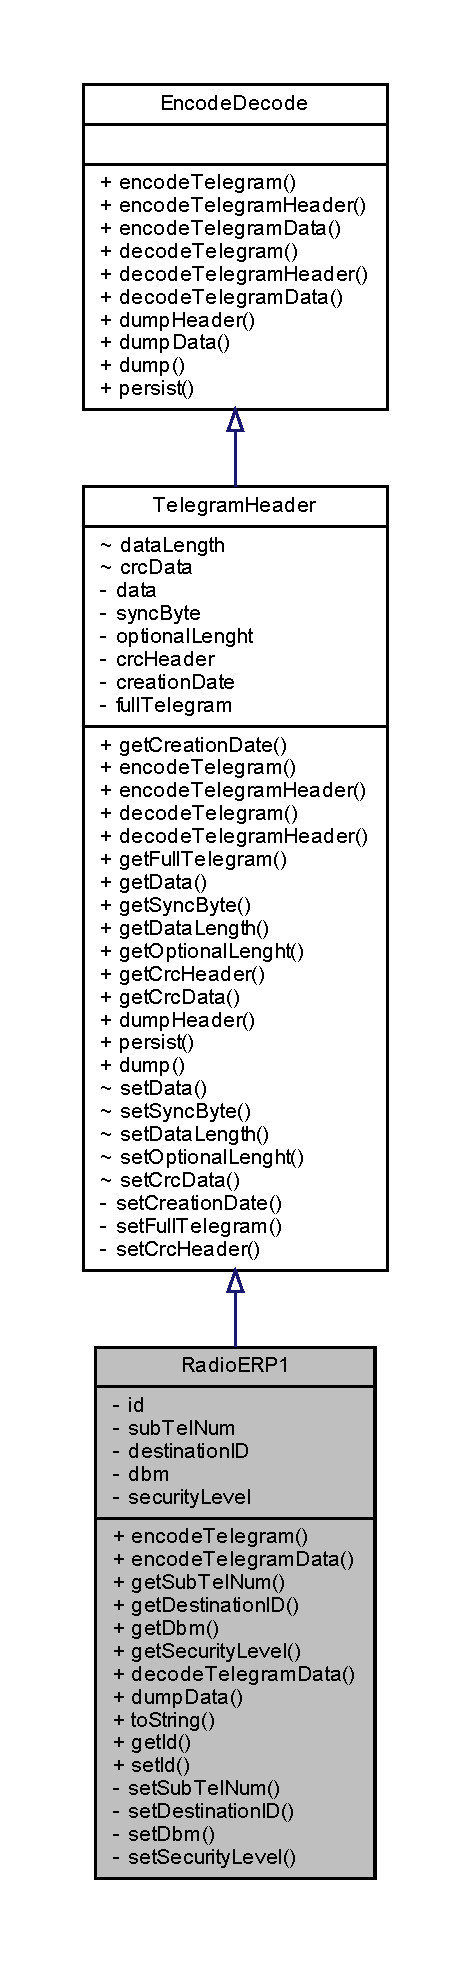
\includegraphics[height=550pt]{df/dea/classch_1_1bfh_1_1gr33nopo55um_1_1enocean_1_1telegram_1_1RadioERP1__inherit__graph}
\end{center}
\end{figure}


Collaboration diagram for Radio\+E\+R\+P1\+:\nopagebreak
\begin{figure}[H]
\begin{center}
\leavevmode
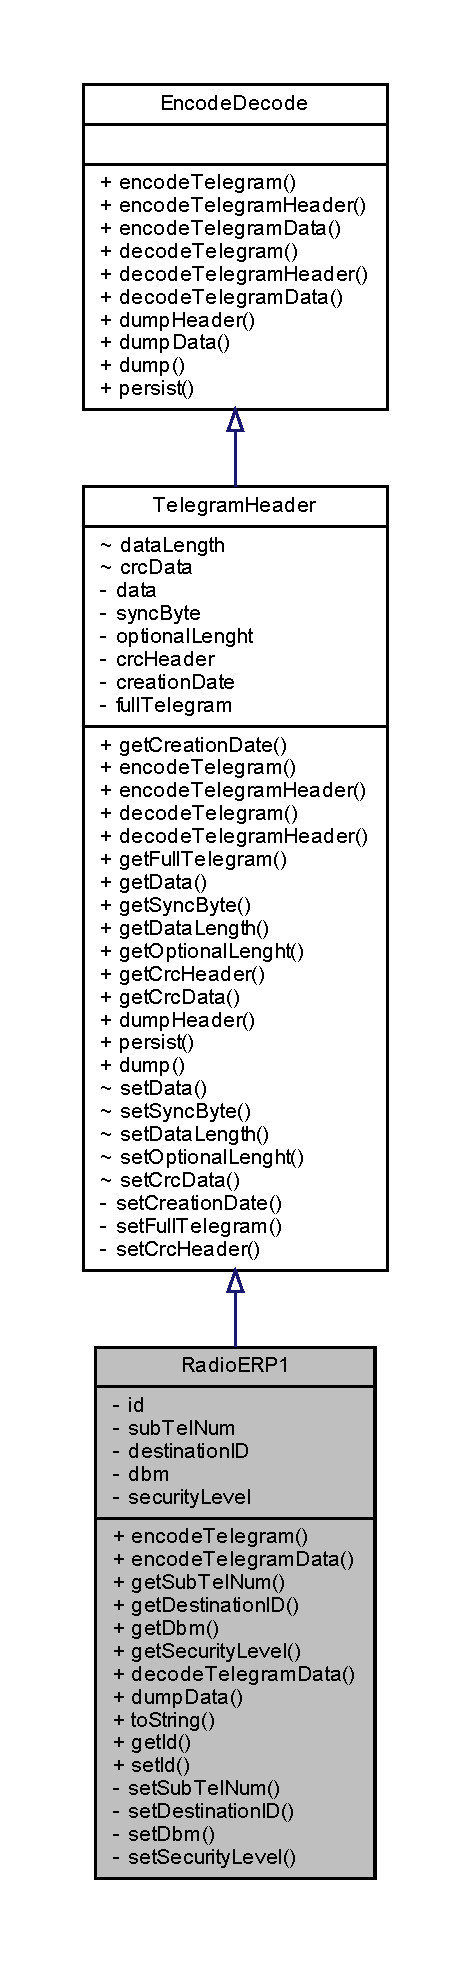
\includegraphics[height=550pt]{de/d7d/classch_1_1bfh_1_1gr33nopo55um_1_1enocean_1_1telegram_1_1RadioERP1__coll__graph}
\end{center}
\end{figure}
\subsection*{Public Member Functions}
\begin{DoxyCompactItemize}
\item 
String {\bf encode\+Telegram} ()
\begin{DoxyCompactList}\small\item\em encode\+Telegram provides an example telegram hex for this packet type. \end{DoxyCompactList}\item 
String {\bf encode\+Telegram\+Data} ()
\begin{DoxyCompactList}\small\item\em encode\+Telegram\+Data provides an example data hex for this packet type. \end{DoxyCompactList}\item 
int {\bf get\+Sub\+Tel\+Num} ()
\item 
String {\bf get\+Destination\+ID} ()
\item 
int {\bf get\+Dbm} ()
\item 
int {\bf get\+Security\+Level} ()
\item 
void {\bf decode\+Telegram\+Data} (String hex\+Telegram)
\begin{DoxyCompactList}\small\item\em decode\+Telegram\+Data splits telegram in parts \end{DoxyCompactList}\item 
void {\bf dump\+Data} ()
\begin{DoxyCompactList}\small\item\em dump\+Data Print Data, useful for logs and testing En\+Ocean Telegram \end{DoxyCompactList}\item 
String {\bf to\+String} ()
\item 
Long {\bf get\+Id} ()
\item 
void {\bf set\+Id} (Long {\bf id})
\end{DoxyCompactItemize}
\subsection*{Private Member Functions}
\begin{DoxyCompactItemize}
\item 
void {\bf set\+Sub\+Tel\+Num} (int {\bf sub\+Tel\+Num})
\item 
void {\bf set\+Destination\+ID} (String {\bf destination\+ID})
\item 
void {\bf set\+Dbm} (int {\bf dbm})
\item 
void {\bf set\+Security\+Level} (int {\bf security\+Level})
\end{DoxyCompactItemize}
\subsection*{Private Attributes}
\begin{DoxyCompactItemize}
\item 
Long {\bf id}
\item 
int {\bf sub\+Tel\+Num}
\item 
String {\bf destination\+ID}
\item 
int {\bf dbm}
\item 
int {\bf security\+Level}
\end{DoxyCompactItemize}
\subsection*{Additional Inherited Members}


\subsection{Detailed Description}


Definition at line {\bf 14} of file {\bf Radio\+E\+R\+P1.\+java}.



\subsection{Member Function Documentation}
\label{classch_1_1bfh_1_1gr33nopo55um_1_1enocean_1_1telegram_1_1RadioERP1_aa581cac5c3efd3142ffa8482079031e9} 
\index{ch\+::bfh\+::gr33nopo55um\+::enocean\+::telegram\+::\+Radio\+E\+R\+P1@{ch\+::bfh\+::gr33nopo55um\+::enocean\+::telegram\+::\+Radio\+E\+R\+P1}!decode\+Telegram\+Data@{decode\+Telegram\+Data}}
\index{decode\+Telegram\+Data@{decode\+Telegram\+Data}!ch\+::bfh\+::gr33nopo55um\+::enocean\+::telegram\+::\+Radio\+E\+R\+P1@{ch\+::bfh\+::gr33nopo55um\+::enocean\+::telegram\+::\+Radio\+E\+R\+P1}}
\subsubsection{decode\+Telegram\+Data()}
{\footnotesize\ttfamily void decode\+Telegram\+Data (\begin{DoxyParamCaption}\item[{String}]{hex\+Telegram }\end{DoxyParamCaption})}



decode\+Telegram\+Data splits telegram in parts 


\begin{DoxyParams}{Parameters}
{\em hex\+Telegram} & in hex String \\
\hline
\end{DoxyParams}


Implements {\bf Encode\+Decode} \doxyref{}{p.}{d1/d8c/interfacech_1_1bfh_1_1gr33nopo55um_1_1enocean_1_1telegram_1_1EncodeDecode_aa581cac5c3efd3142ffa8482079031e9}.



Definition at line {\bf 81} of file {\bf Radio\+E\+R\+P1.\+java}.

Here is the call graph for this function\+:\nopagebreak
\begin{figure}[H]
\begin{center}
\leavevmode
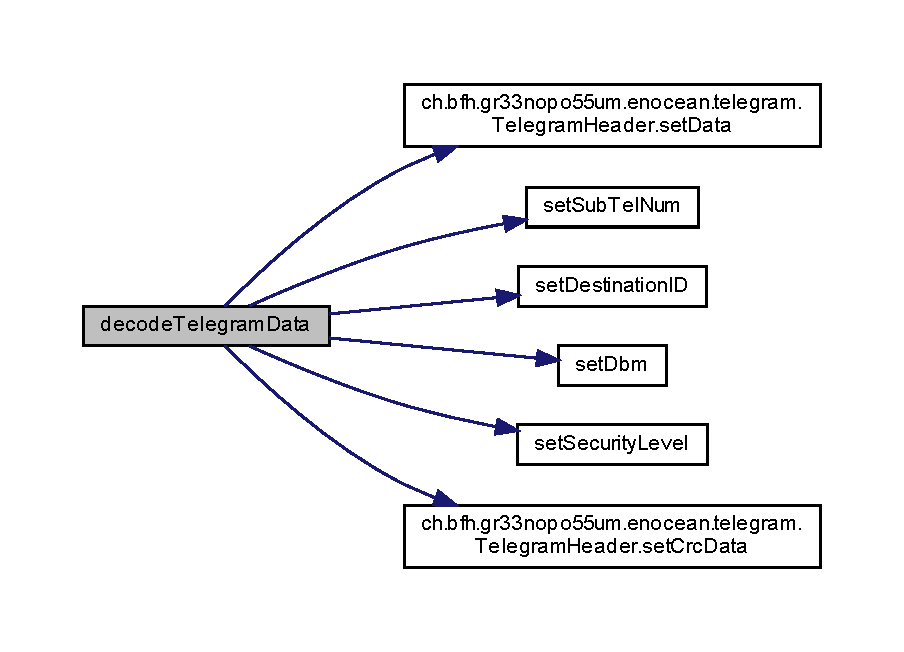
\includegraphics[width=350pt]{d0/d7e/classch_1_1bfh_1_1gr33nopo55um_1_1enocean_1_1telegram_1_1RadioERP1_aa581cac5c3efd3142ffa8482079031e9_cgraph}
\end{center}
\end{figure}
\label{classch_1_1bfh_1_1gr33nopo55um_1_1enocean_1_1telegram_1_1RadioERP1_aff152c0c0c3d5e7011bfff0b9c08032b} 
\index{ch\+::bfh\+::gr33nopo55um\+::enocean\+::telegram\+::\+Radio\+E\+R\+P1@{ch\+::bfh\+::gr33nopo55um\+::enocean\+::telegram\+::\+Radio\+E\+R\+P1}!dump\+Data@{dump\+Data}}
\index{dump\+Data@{dump\+Data}!ch\+::bfh\+::gr33nopo55um\+::enocean\+::telegram\+::\+Radio\+E\+R\+P1@{ch\+::bfh\+::gr33nopo55um\+::enocean\+::telegram\+::\+Radio\+E\+R\+P1}}
\subsubsection{dump\+Data()}
{\footnotesize\ttfamily void dump\+Data (\begin{DoxyParamCaption}{ }\end{DoxyParamCaption})}



dump\+Data Print Data, useful for logs and testing En\+Ocean Telegram 



Implements {\bf Encode\+Decode} \doxyref{}{p.}{d1/d8c/interfacech_1_1bfh_1_1gr33nopo55um_1_1enocean_1_1telegram_1_1EncodeDecode_aff152c0c0c3d5e7011bfff0b9c08032b}.



Definition at line {\bf 98} of file {\bf Radio\+E\+R\+P1.\+java}.

Here is the call graph for this function\+:\nopagebreak
\begin{figure}[H]
\begin{center}
\leavevmode
\includegraphics[width=230pt]{d0/d7e/classch_1_1bfh_1_1gr33nopo55um_1_1enocean_1_1telegram_1_1RadioERP1_aff152c0c0c3d5e7011bfff0b9c08032b_cgraph}
\end{center}
\end{figure}
\label{classch_1_1bfh_1_1gr33nopo55um_1_1enocean_1_1telegram_1_1RadioERP1_a00e3ee3b777334ef3bd46bd4105f9603} 
\index{ch\+::bfh\+::gr33nopo55um\+::enocean\+::telegram\+::\+Radio\+E\+R\+P1@{ch\+::bfh\+::gr33nopo55um\+::enocean\+::telegram\+::\+Radio\+E\+R\+P1}!encode\+Telegram@{encode\+Telegram}}
\index{encode\+Telegram@{encode\+Telegram}!ch\+::bfh\+::gr33nopo55um\+::enocean\+::telegram\+::\+Radio\+E\+R\+P1@{ch\+::bfh\+::gr33nopo55um\+::enocean\+::telegram\+::\+Radio\+E\+R\+P1}}
\subsubsection{encode\+Telegram()}
{\footnotesize\ttfamily String encode\+Telegram (\begin{DoxyParamCaption}{ }\end{DoxyParamCaption})}



encode\+Telegram provides an example telegram hex for this packet type. 

\begin{DoxyReturn}{Returns}
telegram hex 
\end{DoxyReturn}


Implements {\bf Encode\+Decode} \doxyref{}{p.}{d1/d8c/interfacech_1_1bfh_1_1gr33nopo55um_1_1enocean_1_1telegram_1_1EncodeDecode_a00e3ee3b777334ef3bd46bd4105f9603}.



Definition at line {\bf 31} of file {\bf Radio\+E\+R\+P1.\+java}.

\label{classch_1_1bfh_1_1gr33nopo55um_1_1enocean_1_1telegram_1_1RadioERP1_a8a67618ab0362f3d0b60bba6ca93d883} 
\index{ch\+::bfh\+::gr33nopo55um\+::enocean\+::telegram\+::\+Radio\+E\+R\+P1@{ch\+::bfh\+::gr33nopo55um\+::enocean\+::telegram\+::\+Radio\+E\+R\+P1}!encode\+Telegram\+Data@{encode\+Telegram\+Data}}
\index{encode\+Telegram\+Data@{encode\+Telegram\+Data}!ch\+::bfh\+::gr33nopo55um\+::enocean\+::telegram\+::\+Radio\+E\+R\+P1@{ch\+::bfh\+::gr33nopo55um\+::enocean\+::telegram\+::\+Radio\+E\+R\+P1}}
\subsubsection{encode\+Telegram\+Data()}
{\footnotesize\ttfamily String encode\+Telegram\+Data (\begin{DoxyParamCaption}{ }\end{DoxyParamCaption})}



encode\+Telegram\+Data provides an example data hex for this packet type. 

\begin{DoxyReturn}{Returns}
String hex\+Telegram\+Data En\+Ocean Telegram 
\end{DoxyReturn}


Implements {\bf Encode\+Decode} \doxyref{}{p.}{d1/d8c/interfacech_1_1bfh_1_1gr33nopo55um_1_1enocean_1_1telegram_1_1EncodeDecode_a8a67618ab0362f3d0b60bba6ca93d883}.



Definition at line {\bf 40} of file {\bf Radio\+E\+R\+P1.\+java}.

\label{classch_1_1bfh_1_1gr33nopo55um_1_1enocean_1_1telegram_1_1RadioERP1_a41fc3f0b91116ab725e007c5cea15def} 
\index{ch\+::bfh\+::gr33nopo55um\+::enocean\+::telegram\+::\+Radio\+E\+R\+P1@{ch\+::bfh\+::gr33nopo55um\+::enocean\+::telegram\+::\+Radio\+E\+R\+P1}!get\+Dbm@{get\+Dbm}}
\index{get\+Dbm@{get\+Dbm}!ch\+::bfh\+::gr33nopo55um\+::enocean\+::telegram\+::\+Radio\+E\+R\+P1@{ch\+::bfh\+::gr33nopo55um\+::enocean\+::telegram\+::\+Radio\+E\+R\+P1}}
\subsubsection{get\+Dbm()}
{\footnotesize\ttfamily int get\+Dbm (\begin{DoxyParamCaption}{ }\end{DoxyParamCaption})}



Definition at line {\bf 60} of file {\bf Radio\+E\+R\+P1.\+java}.

\label{classch_1_1bfh_1_1gr33nopo55um_1_1enocean_1_1telegram_1_1RadioERP1_ae8e1a722213792caeaeca22c2fd4a672} 
\index{ch\+::bfh\+::gr33nopo55um\+::enocean\+::telegram\+::\+Radio\+E\+R\+P1@{ch\+::bfh\+::gr33nopo55um\+::enocean\+::telegram\+::\+Radio\+E\+R\+P1}!get\+Destination\+ID@{get\+Destination\+ID}}
\index{get\+Destination\+ID@{get\+Destination\+ID}!ch\+::bfh\+::gr33nopo55um\+::enocean\+::telegram\+::\+Radio\+E\+R\+P1@{ch\+::bfh\+::gr33nopo55um\+::enocean\+::telegram\+::\+Radio\+E\+R\+P1}}
\subsubsection{get\+Destination\+I\+D()}
{\footnotesize\ttfamily String get\+Destination\+ID (\begin{DoxyParamCaption}{ }\end{DoxyParamCaption})}



Definition at line {\bf 52} of file {\bf Radio\+E\+R\+P1.\+java}.

\label{classch_1_1bfh_1_1gr33nopo55um_1_1enocean_1_1telegram_1_1RadioERP1_a30e533a51833664ad05441781ee6a6a0} 
\index{ch\+::bfh\+::gr33nopo55um\+::enocean\+::telegram\+::\+Radio\+E\+R\+P1@{ch\+::bfh\+::gr33nopo55um\+::enocean\+::telegram\+::\+Radio\+E\+R\+P1}!get\+Id@{get\+Id}}
\index{get\+Id@{get\+Id}!ch\+::bfh\+::gr33nopo55um\+::enocean\+::telegram\+::\+Radio\+E\+R\+P1@{ch\+::bfh\+::gr33nopo55um\+::enocean\+::telegram\+::\+Radio\+E\+R\+P1}}
\subsubsection{get\+Id()}
{\footnotesize\ttfamily Long get\+Id (\begin{DoxyParamCaption}{ }\end{DoxyParamCaption})}



Definition at line {\bf 114} of file {\bf Radio\+E\+R\+P1.\+java}.

\label{classch_1_1bfh_1_1gr33nopo55um_1_1enocean_1_1telegram_1_1RadioERP1_aba398e80409918bb6ce265a35d558cc1} 
\index{ch\+::bfh\+::gr33nopo55um\+::enocean\+::telegram\+::\+Radio\+E\+R\+P1@{ch\+::bfh\+::gr33nopo55um\+::enocean\+::telegram\+::\+Radio\+E\+R\+P1}!get\+Security\+Level@{get\+Security\+Level}}
\index{get\+Security\+Level@{get\+Security\+Level}!ch\+::bfh\+::gr33nopo55um\+::enocean\+::telegram\+::\+Radio\+E\+R\+P1@{ch\+::bfh\+::gr33nopo55um\+::enocean\+::telegram\+::\+Radio\+E\+R\+P1}}
\subsubsection{get\+Security\+Level()}
{\footnotesize\ttfamily int get\+Security\+Level (\begin{DoxyParamCaption}{ }\end{DoxyParamCaption})}



Definition at line {\bf 68} of file {\bf Radio\+E\+R\+P1.\+java}.

\label{classch_1_1bfh_1_1gr33nopo55um_1_1enocean_1_1telegram_1_1RadioERP1_ae500728eeb6d36d565610634b1f94b5c} 
\index{ch\+::bfh\+::gr33nopo55um\+::enocean\+::telegram\+::\+Radio\+E\+R\+P1@{ch\+::bfh\+::gr33nopo55um\+::enocean\+::telegram\+::\+Radio\+E\+R\+P1}!get\+Sub\+Tel\+Num@{get\+Sub\+Tel\+Num}}
\index{get\+Sub\+Tel\+Num@{get\+Sub\+Tel\+Num}!ch\+::bfh\+::gr33nopo55um\+::enocean\+::telegram\+::\+Radio\+E\+R\+P1@{ch\+::bfh\+::gr33nopo55um\+::enocean\+::telegram\+::\+Radio\+E\+R\+P1}}
\subsubsection{get\+Sub\+Tel\+Num()}
{\footnotesize\ttfamily int get\+Sub\+Tel\+Num (\begin{DoxyParamCaption}{ }\end{DoxyParamCaption})}



Definition at line {\bf 44} of file {\bf Radio\+E\+R\+P1.\+java}.

\label{classch_1_1bfh_1_1gr33nopo55um_1_1enocean_1_1telegram_1_1RadioERP1_a17374793c87ff1a128532736cc1bb082} 
\index{ch\+::bfh\+::gr33nopo55um\+::enocean\+::telegram\+::\+Radio\+E\+R\+P1@{ch\+::bfh\+::gr33nopo55um\+::enocean\+::telegram\+::\+Radio\+E\+R\+P1}!set\+Dbm@{set\+Dbm}}
\index{set\+Dbm@{set\+Dbm}!ch\+::bfh\+::gr33nopo55um\+::enocean\+::telegram\+::\+Radio\+E\+R\+P1@{ch\+::bfh\+::gr33nopo55um\+::enocean\+::telegram\+::\+Radio\+E\+R\+P1}}
\subsubsection{set\+Dbm()}
{\footnotesize\ttfamily void set\+Dbm (\begin{DoxyParamCaption}\item[{int}]{dbm }\end{DoxyParamCaption})\hspace{0.3cm}{\ttfamily [private]}}



Definition at line {\bf 64} of file {\bf Radio\+E\+R\+P1.\+java}.

Here is the caller graph for this function\+:\nopagebreak
\begin{figure}[H]
\begin{center}
\leavevmode
\includegraphics[width=286pt]{d0/d7e/classch_1_1bfh_1_1gr33nopo55um_1_1enocean_1_1telegram_1_1RadioERP1_a17374793c87ff1a128532736cc1bb082_icgraph}
\end{center}
\end{figure}
\label{classch_1_1bfh_1_1gr33nopo55um_1_1enocean_1_1telegram_1_1RadioERP1_a0adf8d36cde20c0aa200903cd150803d} 
\index{ch\+::bfh\+::gr33nopo55um\+::enocean\+::telegram\+::\+Radio\+E\+R\+P1@{ch\+::bfh\+::gr33nopo55um\+::enocean\+::telegram\+::\+Radio\+E\+R\+P1}!set\+Destination\+ID@{set\+Destination\+ID}}
\index{set\+Destination\+ID@{set\+Destination\+ID}!ch\+::bfh\+::gr33nopo55um\+::enocean\+::telegram\+::\+Radio\+E\+R\+P1@{ch\+::bfh\+::gr33nopo55um\+::enocean\+::telegram\+::\+Radio\+E\+R\+P1}}
\subsubsection{set\+Destination\+I\+D()}
{\footnotesize\ttfamily void set\+Destination\+ID (\begin{DoxyParamCaption}\item[{String}]{destination\+ID }\end{DoxyParamCaption})\hspace{0.3cm}{\ttfamily [private]}}



Definition at line {\bf 56} of file {\bf Radio\+E\+R\+P1.\+java}.

Here is the caller graph for this function\+:\nopagebreak
\begin{figure}[H]
\begin{center}
\leavevmode
\includegraphics[width=324pt]{d0/d7e/classch_1_1bfh_1_1gr33nopo55um_1_1enocean_1_1telegram_1_1RadioERP1_a0adf8d36cde20c0aa200903cd150803d_icgraph}
\end{center}
\end{figure}
\label{classch_1_1bfh_1_1gr33nopo55um_1_1enocean_1_1telegram_1_1RadioERP1_ae855b9b14d52c956a065d1a71f74a136} 
\index{ch\+::bfh\+::gr33nopo55um\+::enocean\+::telegram\+::\+Radio\+E\+R\+P1@{ch\+::bfh\+::gr33nopo55um\+::enocean\+::telegram\+::\+Radio\+E\+R\+P1}!set\+Id@{set\+Id}}
\index{set\+Id@{set\+Id}!ch\+::bfh\+::gr33nopo55um\+::enocean\+::telegram\+::\+Radio\+E\+R\+P1@{ch\+::bfh\+::gr33nopo55um\+::enocean\+::telegram\+::\+Radio\+E\+R\+P1}}
\subsubsection{set\+Id()}
{\footnotesize\ttfamily void set\+Id (\begin{DoxyParamCaption}\item[{Long}]{id }\end{DoxyParamCaption})}



Definition at line {\bf 118} of file {\bf Radio\+E\+R\+P1.\+java}.

\label{classch_1_1bfh_1_1gr33nopo55um_1_1enocean_1_1telegram_1_1RadioERP1_acf57a842678a18a5a9fdcb089b4efee2} 
\index{ch\+::bfh\+::gr33nopo55um\+::enocean\+::telegram\+::\+Radio\+E\+R\+P1@{ch\+::bfh\+::gr33nopo55um\+::enocean\+::telegram\+::\+Radio\+E\+R\+P1}!set\+Security\+Level@{set\+Security\+Level}}
\index{set\+Security\+Level@{set\+Security\+Level}!ch\+::bfh\+::gr33nopo55um\+::enocean\+::telegram\+::\+Radio\+E\+R\+P1@{ch\+::bfh\+::gr33nopo55um\+::enocean\+::telegram\+::\+Radio\+E\+R\+P1}}
\subsubsection{set\+Security\+Level()}
{\footnotesize\ttfamily void set\+Security\+Level (\begin{DoxyParamCaption}\item[{int}]{security\+Level }\end{DoxyParamCaption})\hspace{0.3cm}{\ttfamily [private]}}



Definition at line {\bf 72} of file {\bf Radio\+E\+R\+P1.\+java}.

Here is the caller graph for this function\+:\nopagebreak
\begin{figure}[H]
\begin{center}
\leavevmode
\includegraphics[width=325pt]{d0/d7e/classch_1_1bfh_1_1gr33nopo55um_1_1enocean_1_1telegram_1_1RadioERP1_acf57a842678a18a5a9fdcb089b4efee2_icgraph}
\end{center}
\end{figure}
\label{classch_1_1bfh_1_1gr33nopo55um_1_1enocean_1_1telegram_1_1RadioERP1_a5bfc8ac914e36e7e37b467fdcd90dbda} 
\index{ch\+::bfh\+::gr33nopo55um\+::enocean\+::telegram\+::\+Radio\+E\+R\+P1@{ch\+::bfh\+::gr33nopo55um\+::enocean\+::telegram\+::\+Radio\+E\+R\+P1}!set\+Sub\+Tel\+Num@{set\+Sub\+Tel\+Num}}
\index{set\+Sub\+Tel\+Num@{set\+Sub\+Tel\+Num}!ch\+::bfh\+::gr33nopo55um\+::enocean\+::telegram\+::\+Radio\+E\+R\+P1@{ch\+::bfh\+::gr33nopo55um\+::enocean\+::telegram\+::\+Radio\+E\+R\+P1}}
\subsubsection{set\+Sub\+Tel\+Num()}
{\footnotesize\ttfamily void set\+Sub\+Tel\+Num (\begin{DoxyParamCaption}\item[{int}]{sub\+Tel\+Num }\end{DoxyParamCaption})\hspace{0.3cm}{\ttfamily [private]}}



Definition at line {\bf 48} of file {\bf Radio\+E\+R\+P1.\+java}.

Here is the caller graph for this function\+:\nopagebreak
\begin{figure}[H]
\begin{center}
\leavevmode
\includegraphics[width=317pt]{d0/d7e/classch_1_1bfh_1_1gr33nopo55um_1_1enocean_1_1telegram_1_1RadioERP1_a5bfc8ac914e36e7e37b467fdcd90dbda_icgraph}
\end{center}
\end{figure}
\label{classch_1_1bfh_1_1gr33nopo55um_1_1enocean_1_1telegram_1_1RadioERP1_ad146fa8579a5f8a876c4688cc5a68520} 
\index{ch\+::bfh\+::gr33nopo55um\+::enocean\+::telegram\+::\+Radio\+E\+R\+P1@{ch\+::bfh\+::gr33nopo55um\+::enocean\+::telegram\+::\+Radio\+E\+R\+P1}!to\+String@{to\+String}}
\index{to\+String@{to\+String}!ch\+::bfh\+::gr33nopo55um\+::enocean\+::telegram\+::\+Radio\+E\+R\+P1@{ch\+::bfh\+::gr33nopo55um\+::enocean\+::telegram\+::\+Radio\+E\+R\+P1}}
\subsubsection{to\+String()}
{\footnotesize\ttfamily String to\+String (\begin{DoxyParamCaption}{ }\end{DoxyParamCaption})}



Definition at line {\bf 105} of file {\bf Radio\+E\+R\+P1.\+java}.

Here is the caller graph for this function\+:\nopagebreak
\begin{figure}[H]
\begin{center}
\leavevmode
\includegraphics[width=230pt]{d0/d7e/classch_1_1bfh_1_1gr33nopo55um_1_1enocean_1_1telegram_1_1RadioERP1_ad146fa8579a5f8a876c4688cc5a68520_icgraph}
\end{center}
\end{figure}


\subsection{Member Data Documentation}
\label{classch_1_1bfh_1_1gr33nopo55um_1_1enocean_1_1telegram_1_1RadioERP1_ad2c3b8f9fd4bbc30208e66b69c290dc6} 
\index{ch\+::bfh\+::gr33nopo55um\+::enocean\+::telegram\+::\+Radio\+E\+R\+P1@{ch\+::bfh\+::gr33nopo55um\+::enocean\+::telegram\+::\+Radio\+E\+R\+P1}!dbm@{dbm}}
\index{dbm@{dbm}!ch\+::bfh\+::gr33nopo55um\+::enocean\+::telegram\+::\+Radio\+E\+R\+P1@{ch\+::bfh\+::gr33nopo55um\+::enocean\+::telegram\+::\+Radio\+E\+R\+P1}}
\subsubsection{dbm}
{\footnotesize\ttfamily int dbm\hspace{0.3cm}{\ttfamily [private]}}



Definition at line {\bf 22} of file {\bf Radio\+E\+R\+P1.\+java}.

\label{classch_1_1bfh_1_1gr33nopo55um_1_1enocean_1_1telegram_1_1RadioERP1_aa6aa9318a98d6578ce0ad9aeab2eff06} 
\index{ch\+::bfh\+::gr33nopo55um\+::enocean\+::telegram\+::\+Radio\+E\+R\+P1@{ch\+::bfh\+::gr33nopo55um\+::enocean\+::telegram\+::\+Radio\+E\+R\+P1}!destination\+ID@{destination\+ID}}
\index{destination\+ID@{destination\+ID}!ch\+::bfh\+::gr33nopo55um\+::enocean\+::telegram\+::\+Radio\+E\+R\+P1@{ch\+::bfh\+::gr33nopo55um\+::enocean\+::telegram\+::\+Radio\+E\+R\+P1}}
\subsubsection{destination\+ID}
{\footnotesize\ttfamily String destination\+ID\hspace{0.3cm}{\ttfamily [private]}}



Definition at line {\bf 21} of file {\bf Radio\+E\+R\+P1.\+java}.

\label{classch_1_1bfh_1_1gr33nopo55um_1_1enocean_1_1telegram_1_1RadioERP1_afdea3f4ac85ac5819c978584be2be48e} 
\index{ch\+::bfh\+::gr33nopo55um\+::enocean\+::telegram\+::\+Radio\+E\+R\+P1@{ch\+::bfh\+::gr33nopo55um\+::enocean\+::telegram\+::\+Radio\+E\+R\+P1}!id@{id}}
\index{id@{id}!ch\+::bfh\+::gr33nopo55um\+::enocean\+::telegram\+::\+Radio\+E\+R\+P1@{ch\+::bfh\+::gr33nopo55um\+::enocean\+::telegram\+::\+Radio\+E\+R\+P1}}
\subsubsection{id}
{\footnotesize\ttfamily Long id\hspace{0.3cm}{\ttfamily [private]}}



Definition at line {\bf 18} of file {\bf Radio\+E\+R\+P1.\+java}.

\label{classch_1_1bfh_1_1gr33nopo55um_1_1enocean_1_1telegram_1_1RadioERP1_a284d5e19f68e1381c69905da7e5df7f2} 
\index{ch\+::bfh\+::gr33nopo55um\+::enocean\+::telegram\+::\+Radio\+E\+R\+P1@{ch\+::bfh\+::gr33nopo55um\+::enocean\+::telegram\+::\+Radio\+E\+R\+P1}!security\+Level@{security\+Level}}
\index{security\+Level@{security\+Level}!ch\+::bfh\+::gr33nopo55um\+::enocean\+::telegram\+::\+Radio\+E\+R\+P1@{ch\+::bfh\+::gr33nopo55um\+::enocean\+::telegram\+::\+Radio\+E\+R\+P1}}
\subsubsection{security\+Level}
{\footnotesize\ttfamily int security\+Level\hspace{0.3cm}{\ttfamily [private]}}



Definition at line {\bf 23} of file {\bf Radio\+E\+R\+P1.\+java}.

\label{classch_1_1bfh_1_1gr33nopo55um_1_1enocean_1_1telegram_1_1RadioERP1_a00f71ebf2ba1bdafe87d7bb738e50194} 
\index{ch\+::bfh\+::gr33nopo55um\+::enocean\+::telegram\+::\+Radio\+E\+R\+P1@{ch\+::bfh\+::gr33nopo55um\+::enocean\+::telegram\+::\+Radio\+E\+R\+P1}!sub\+Tel\+Num@{sub\+Tel\+Num}}
\index{sub\+Tel\+Num@{sub\+Tel\+Num}!ch\+::bfh\+::gr33nopo55um\+::enocean\+::telegram\+::\+Radio\+E\+R\+P1@{ch\+::bfh\+::gr33nopo55um\+::enocean\+::telegram\+::\+Radio\+E\+R\+P1}}
\subsubsection{sub\+Tel\+Num}
{\footnotesize\ttfamily int sub\+Tel\+Num\hspace{0.3cm}{\ttfamily [private]}}



Definition at line {\bf 20} of file {\bf Radio\+E\+R\+P1.\+java}.



The documentation for this class was generated from the following file\+:\begin{DoxyCompactItemize}
\item 
/home/silas/\+Idea\+Projects/\+En\+Ocean/src/ch/bfh/gr33nopo55um/enocean/telegram/{\bf Radio\+E\+R\+P1.\+java}\end{DoxyCompactItemize}

\section{Radio\+E\+R\+P2}
\label{classch_1_1bfh_1_1gr33nopo55um_1_1enocean_1_1telegram_1_1RadioERP2}\index{Radio\+E\+R\+P2@{Radio\+E\+R\+P2}}


Inheritance diagram for Radio\+E\+R\+P2\+:\nopagebreak
\begin{figure}[H]
\begin{center}
\leavevmode
\includegraphics[height=550pt]{dc/d83/classch_1_1bfh_1_1gr33nopo55um_1_1enocean_1_1telegram_1_1RadioERP2__inherit__graph}
\end{center}
\end{figure}


Collaboration diagram for Radio\+E\+R\+P2\+:\nopagebreak
\begin{figure}[H]
\begin{center}
\leavevmode
\includegraphics[height=550pt]{d0/dc3/classch_1_1bfh_1_1gr33nopo55um_1_1enocean_1_1telegram_1_1RadioERP2__coll__graph}
\end{center}
\end{figure}
\subsection*{Public Member Functions}
\begin{DoxyCompactItemize}
\item 
String {\bf encode\+Telegram} ()
\begin{DoxyCompactList}\small\item\em encode\+Telegram provides an example telegram hex for this packet type. \end{DoxyCompactList}\item 
String {\bf encode\+Telegram\+Data} ()
\begin{DoxyCompactList}\small\item\em encode\+Telegram\+Data provides an example data hex for this packet type. \end{DoxyCompactList}\item 
void {\bf decode\+Telegram\+Data} (String hex\+Telegram)
\begin{DoxyCompactList}\small\item\em decode\+Telegram\+Data splits telegram in parts \end{DoxyCompactList}\item 
int {\bf get\+Sub\+Tel\+Num} ()
\item 
int {\bf get\+Dbm} ()
\item 
String {\bf get\+Raw\+Data} ()
\item 
void {\bf dump\+Data} ()
\begin{DoxyCompactList}\small\item\em dump\+Data Print Data, useful for logs and testing En\+Ocean Telegram \end{DoxyCompactList}\item 
String {\bf to\+String} ()
\item 
Long {\bf get\+Id} ()
\item 
void {\bf set\+Id} (Long {\bf id})
\end{DoxyCompactItemize}
\subsection*{Private Member Functions}
\begin{DoxyCompactItemize}
\item 
void {\bf set\+Sub\+Tel\+Num} (int {\bf sub\+Tel\+Num})
\item 
void {\bf set\+Dbm} (int {\bf dbm})
\item 
void {\bf set\+Raw\+Data} (String {\bf raw\+Data})
\end{DoxyCompactItemize}
\subsection*{Private Attributes}
\begin{DoxyCompactItemize}
\item 
Long {\bf id}
\item 
int {\bf sub\+Tel\+Num}
\item 
int {\bf dbm}
\item 
String {\bf raw\+Data}
\end{DoxyCompactItemize}
\subsection*{Additional Inherited Members}


\subsection{Detailed Description}


Definition at line {\bf 14} of file {\bf Radio\+E\+R\+P2.\+java}.



\subsection{Member Function Documentation}
\label{classch_1_1bfh_1_1gr33nopo55um_1_1enocean_1_1telegram_1_1RadioERP2_aa581cac5c3efd3142ffa8482079031e9} 
\index{ch\+::bfh\+::gr33nopo55um\+::enocean\+::telegram\+::\+Radio\+E\+R\+P2@{ch\+::bfh\+::gr33nopo55um\+::enocean\+::telegram\+::\+Radio\+E\+R\+P2}!decode\+Telegram\+Data@{decode\+Telegram\+Data}}
\index{decode\+Telegram\+Data@{decode\+Telegram\+Data}!ch\+::bfh\+::gr33nopo55um\+::enocean\+::telegram\+::\+Radio\+E\+R\+P2@{ch\+::bfh\+::gr33nopo55um\+::enocean\+::telegram\+::\+Radio\+E\+R\+P2}}
\subsubsection{decode\+Telegram\+Data()}
{\footnotesize\ttfamily void decode\+Telegram\+Data (\begin{DoxyParamCaption}\item[{String}]{hex\+Telegram }\end{DoxyParamCaption})}



decode\+Telegram\+Data splits telegram in parts 


\begin{DoxyParams}{Parameters}
{\em hex\+Telegram} & in hex String \\
\hline
\end{DoxyParams}


Implements {\bf Encode\+Decode} \doxyref{}{p.}{d1/d8c/interfacech_1_1bfh_1_1gr33nopo55um_1_1enocean_1_1telegram_1_1EncodeDecode_aa581cac5c3efd3142ffa8482079031e9}.



Definition at line {\bf 53} of file {\bf Radio\+E\+R\+P2.\+java}.

Here is the call graph for this function\+:\nopagebreak
\begin{figure}[H]
\begin{center}
\leavevmode
\includegraphics[width=350pt]{d6/d05/classch_1_1bfh_1_1gr33nopo55um_1_1enocean_1_1telegram_1_1RadioERP2_aa581cac5c3efd3142ffa8482079031e9_cgraph}
\end{center}
\end{figure}
\label{classch_1_1bfh_1_1gr33nopo55um_1_1enocean_1_1telegram_1_1RadioERP2_aff152c0c0c3d5e7011bfff0b9c08032b} 
\index{ch\+::bfh\+::gr33nopo55um\+::enocean\+::telegram\+::\+Radio\+E\+R\+P2@{ch\+::bfh\+::gr33nopo55um\+::enocean\+::telegram\+::\+Radio\+E\+R\+P2}!dump\+Data@{dump\+Data}}
\index{dump\+Data@{dump\+Data}!ch\+::bfh\+::gr33nopo55um\+::enocean\+::telegram\+::\+Radio\+E\+R\+P2@{ch\+::bfh\+::gr33nopo55um\+::enocean\+::telegram\+::\+Radio\+E\+R\+P2}}
\subsubsection{dump\+Data()}
{\footnotesize\ttfamily void dump\+Data (\begin{DoxyParamCaption}{ }\end{DoxyParamCaption})}



dump\+Data Print Data, useful for logs and testing En\+Ocean Telegram 



Implements {\bf Encode\+Decode} \doxyref{}{p.}{d1/d8c/interfacech_1_1bfh_1_1gr33nopo55um_1_1enocean_1_1telegram_1_1EncodeDecode_aff152c0c0c3d5e7011bfff0b9c08032b}.



Definition at line {\bf 92} of file {\bf Radio\+E\+R\+P2.\+java}.

Here is the call graph for this function\+:\nopagebreak
\begin{figure}[H]
\begin{center}
\leavevmode
\includegraphics[width=230pt]{d6/d05/classch_1_1bfh_1_1gr33nopo55um_1_1enocean_1_1telegram_1_1RadioERP2_aff152c0c0c3d5e7011bfff0b9c08032b_cgraph}
\end{center}
\end{figure}
\label{classch_1_1bfh_1_1gr33nopo55um_1_1enocean_1_1telegram_1_1RadioERP2_a00e3ee3b777334ef3bd46bd4105f9603} 
\index{ch\+::bfh\+::gr33nopo55um\+::enocean\+::telegram\+::\+Radio\+E\+R\+P2@{ch\+::bfh\+::gr33nopo55um\+::enocean\+::telegram\+::\+Radio\+E\+R\+P2}!encode\+Telegram@{encode\+Telegram}}
\index{encode\+Telegram@{encode\+Telegram}!ch\+::bfh\+::gr33nopo55um\+::enocean\+::telegram\+::\+Radio\+E\+R\+P2@{ch\+::bfh\+::gr33nopo55um\+::enocean\+::telegram\+::\+Radio\+E\+R\+P2}}
\subsubsection{encode\+Telegram()}
{\footnotesize\ttfamily String encode\+Telegram (\begin{DoxyParamCaption}{ }\end{DoxyParamCaption})}



encode\+Telegram provides an example telegram hex for this packet type. 

\begin{DoxyReturn}{Returns}
telegram hex 
\end{DoxyReturn}


Implements {\bf Encode\+Decode} \doxyref{}{p.}{d1/d8c/interfacech_1_1bfh_1_1gr33nopo55um_1_1enocean_1_1telegram_1_1EncodeDecode_a00e3ee3b777334ef3bd46bd4105f9603}.



Definition at line {\bf 33} of file {\bf Radio\+E\+R\+P2.\+java}.

\label{classch_1_1bfh_1_1gr33nopo55um_1_1enocean_1_1telegram_1_1RadioERP2_a8a67618ab0362f3d0b60bba6ca93d883} 
\index{ch\+::bfh\+::gr33nopo55um\+::enocean\+::telegram\+::\+Radio\+E\+R\+P2@{ch\+::bfh\+::gr33nopo55um\+::enocean\+::telegram\+::\+Radio\+E\+R\+P2}!encode\+Telegram\+Data@{encode\+Telegram\+Data}}
\index{encode\+Telegram\+Data@{encode\+Telegram\+Data}!ch\+::bfh\+::gr33nopo55um\+::enocean\+::telegram\+::\+Radio\+E\+R\+P2@{ch\+::bfh\+::gr33nopo55um\+::enocean\+::telegram\+::\+Radio\+E\+R\+P2}}
\subsubsection{encode\+Telegram\+Data()}
{\footnotesize\ttfamily String encode\+Telegram\+Data (\begin{DoxyParamCaption}{ }\end{DoxyParamCaption})}



encode\+Telegram\+Data provides an example data hex for this packet type. 

\begin{DoxyReturn}{Returns}
String hex\+Telegram\+Data En\+Ocean Telegram 
\end{DoxyReturn}


Implements {\bf Encode\+Decode} \doxyref{}{p.}{d1/d8c/interfacech_1_1bfh_1_1gr33nopo55um_1_1enocean_1_1telegram_1_1EncodeDecode_a8a67618ab0362f3d0b60bba6ca93d883}.



Definition at line {\bf 43} of file {\bf Radio\+E\+R\+P2.\+java}.

\label{classch_1_1bfh_1_1gr33nopo55um_1_1enocean_1_1telegram_1_1RadioERP2_a41fc3f0b91116ab725e007c5cea15def} 
\index{ch\+::bfh\+::gr33nopo55um\+::enocean\+::telegram\+::\+Radio\+E\+R\+P2@{ch\+::bfh\+::gr33nopo55um\+::enocean\+::telegram\+::\+Radio\+E\+R\+P2}!get\+Dbm@{get\+Dbm}}
\index{get\+Dbm@{get\+Dbm}!ch\+::bfh\+::gr33nopo55um\+::enocean\+::telegram\+::\+Radio\+E\+R\+P2@{ch\+::bfh\+::gr33nopo55um\+::enocean\+::telegram\+::\+Radio\+E\+R\+P2}}
\subsubsection{get\+Dbm()}
{\footnotesize\ttfamily int get\+Dbm (\begin{DoxyParamCaption}{ }\end{DoxyParamCaption})}



Definition at line {\bf 74} of file {\bf Radio\+E\+R\+P2.\+java}.

\label{classch_1_1bfh_1_1gr33nopo55um_1_1enocean_1_1telegram_1_1RadioERP2_a30e533a51833664ad05441781ee6a6a0} 
\index{ch\+::bfh\+::gr33nopo55um\+::enocean\+::telegram\+::\+Radio\+E\+R\+P2@{ch\+::bfh\+::gr33nopo55um\+::enocean\+::telegram\+::\+Radio\+E\+R\+P2}!get\+Id@{get\+Id}}
\index{get\+Id@{get\+Id}!ch\+::bfh\+::gr33nopo55um\+::enocean\+::telegram\+::\+Radio\+E\+R\+P2@{ch\+::bfh\+::gr33nopo55um\+::enocean\+::telegram\+::\+Radio\+E\+R\+P2}}
\subsubsection{get\+Id()}
{\footnotesize\ttfamily Long get\+Id (\begin{DoxyParamCaption}{ }\end{DoxyParamCaption})}



Definition at line {\bf 106} of file {\bf Radio\+E\+R\+P2.\+java}.

\label{classch_1_1bfh_1_1gr33nopo55um_1_1enocean_1_1telegram_1_1RadioERP2_ae7bc1ea8df3c210a1618f7a87e5e1297} 
\index{ch\+::bfh\+::gr33nopo55um\+::enocean\+::telegram\+::\+Radio\+E\+R\+P2@{ch\+::bfh\+::gr33nopo55um\+::enocean\+::telegram\+::\+Radio\+E\+R\+P2}!get\+Raw\+Data@{get\+Raw\+Data}}
\index{get\+Raw\+Data@{get\+Raw\+Data}!ch\+::bfh\+::gr33nopo55um\+::enocean\+::telegram\+::\+Radio\+E\+R\+P2@{ch\+::bfh\+::gr33nopo55um\+::enocean\+::telegram\+::\+Radio\+E\+R\+P2}}
\subsubsection{get\+Raw\+Data()}
{\footnotesize\ttfamily String get\+Raw\+Data (\begin{DoxyParamCaption}{ }\end{DoxyParamCaption})}



Definition at line {\bf 82} of file {\bf Radio\+E\+R\+P2.\+java}.

\label{classch_1_1bfh_1_1gr33nopo55um_1_1enocean_1_1telegram_1_1RadioERP2_ae500728eeb6d36d565610634b1f94b5c} 
\index{ch\+::bfh\+::gr33nopo55um\+::enocean\+::telegram\+::\+Radio\+E\+R\+P2@{ch\+::bfh\+::gr33nopo55um\+::enocean\+::telegram\+::\+Radio\+E\+R\+P2}!get\+Sub\+Tel\+Num@{get\+Sub\+Tel\+Num}}
\index{get\+Sub\+Tel\+Num@{get\+Sub\+Tel\+Num}!ch\+::bfh\+::gr33nopo55um\+::enocean\+::telegram\+::\+Radio\+E\+R\+P2@{ch\+::bfh\+::gr33nopo55um\+::enocean\+::telegram\+::\+Radio\+E\+R\+P2}}
\subsubsection{get\+Sub\+Tel\+Num()}
{\footnotesize\ttfamily int get\+Sub\+Tel\+Num (\begin{DoxyParamCaption}{ }\end{DoxyParamCaption})}

\begin{DoxyReturn}{Returns}
sub\+Tel\+Num 
\end{DoxyReturn}


Definition at line {\bf 66} of file {\bf Radio\+E\+R\+P2.\+java}.

\label{classch_1_1bfh_1_1gr33nopo55um_1_1enocean_1_1telegram_1_1RadioERP2_a17374793c87ff1a128532736cc1bb082} 
\index{ch\+::bfh\+::gr33nopo55um\+::enocean\+::telegram\+::\+Radio\+E\+R\+P2@{ch\+::bfh\+::gr33nopo55um\+::enocean\+::telegram\+::\+Radio\+E\+R\+P2}!set\+Dbm@{set\+Dbm}}
\index{set\+Dbm@{set\+Dbm}!ch\+::bfh\+::gr33nopo55um\+::enocean\+::telegram\+::\+Radio\+E\+R\+P2@{ch\+::bfh\+::gr33nopo55um\+::enocean\+::telegram\+::\+Radio\+E\+R\+P2}}
\subsubsection{set\+Dbm()}
{\footnotesize\ttfamily void set\+Dbm (\begin{DoxyParamCaption}\item[{int}]{dbm }\end{DoxyParamCaption})\hspace{0.3cm}{\ttfamily [private]}}



Definition at line {\bf 78} of file {\bf Radio\+E\+R\+P2.\+java}.

Here is the caller graph for this function\+:\nopagebreak
\begin{figure}[H]
\begin{center}
\leavevmode
\includegraphics[width=286pt]{d6/d05/classch_1_1bfh_1_1gr33nopo55um_1_1enocean_1_1telegram_1_1RadioERP2_a17374793c87ff1a128532736cc1bb082_icgraph}
\end{center}
\end{figure}
\label{classch_1_1bfh_1_1gr33nopo55um_1_1enocean_1_1telegram_1_1RadioERP2_ae855b9b14d52c956a065d1a71f74a136} 
\index{ch\+::bfh\+::gr33nopo55um\+::enocean\+::telegram\+::\+Radio\+E\+R\+P2@{ch\+::bfh\+::gr33nopo55um\+::enocean\+::telegram\+::\+Radio\+E\+R\+P2}!set\+Id@{set\+Id}}
\index{set\+Id@{set\+Id}!ch\+::bfh\+::gr33nopo55um\+::enocean\+::telegram\+::\+Radio\+E\+R\+P2@{ch\+::bfh\+::gr33nopo55um\+::enocean\+::telegram\+::\+Radio\+E\+R\+P2}}
\subsubsection{set\+Id()}
{\footnotesize\ttfamily void set\+Id (\begin{DoxyParamCaption}\item[{Long}]{id }\end{DoxyParamCaption})}



Definition at line {\bf 110} of file {\bf Radio\+E\+R\+P2.\+java}.

\label{classch_1_1bfh_1_1gr33nopo55um_1_1enocean_1_1telegram_1_1RadioERP2_ae01d76ba5f87f8c57834b729295a18df} 
\index{ch\+::bfh\+::gr33nopo55um\+::enocean\+::telegram\+::\+Radio\+E\+R\+P2@{ch\+::bfh\+::gr33nopo55um\+::enocean\+::telegram\+::\+Radio\+E\+R\+P2}!set\+Raw\+Data@{set\+Raw\+Data}}
\index{set\+Raw\+Data@{set\+Raw\+Data}!ch\+::bfh\+::gr33nopo55um\+::enocean\+::telegram\+::\+Radio\+E\+R\+P2@{ch\+::bfh\+::gr33nopo55um\+::enocean\+::telegram\+::\+Radio\+E\+R\+P2}}
\subsubsection{set\+Raw\+Data()}
{\footnotesize\ttfamily void set\+Raw\+Data (\begin{DoxyParamCaption}\item[{String}]{raw\+Data }\end{DoxyParamCaption})\hspace{0.3cm}{\ttfamily [private]}}



Definition at line {\bf 86} of file {\bf Radio\+E\+R\+P2.\+java}.

Here is the caller graph for this function\+:\nopagebreak
\begin{figure}[H]
\begin{center}
\leavevmode
\includegraphics[width=305pt]{d6/d05/classch_1_1bfh_1_1gr33nopo55um_1_1enocean_1_1telegram_1_1RadioERP2_ae01d76ba5f87f8c57834b729295a18df_icgraph}
\end{center}
\end{figure}
\label{classch_1_1bfh_1_1gr33nopo55um_1_1enocean_1_1telegram_1_1RadioERP2_a5bfc8ac914e36e7e37b467fdcd90dbda} 
\index{ch\+::bfh\+::gr33nopo55um\+::enocean\+::telegram\+::\+Radio\+E\+R\+P2@{ch\+::bfh\+::gr33nopo55um\+::enocean\+::telegram\+::\+Radio\+E\+R\+P2}!set\+Sub\+Tel\+Num@{set\+Sub\+Tel\+Num}}
\index{set\+Sub\+Tel\+Num@{set\+Sub\+Tel\+Num}!ch\+::bfh\+::gr33nopo55um\+::enocean\+::telegram\+::\+Radio\+E\+R\+P2@{ch\+::bfh\+::gr33nopo55um\+::enocean\+::telegram\+::\+Radio\+E\+R\+P2}}
\subsubsection{set\+Sub\+Tel\+Num()}
{\footnotesize\ttfamily void set\+Sub\+Tel\+Num (\begin{DoxyParamCaption}\item[{int}]{sub\+Tel\+Num }\end{DoxyParamCaption})\hspace{0.3cm}{\ttfamily [private]}}



Definition at line {\bf 70} of file {\bf Radio\+E\+R\+P2.\+java}.

Here is the caller graph for this function\+:\nopagebreak
\begin{figure}[H]
\begin{center}
\leavevmode
\includegraphics[width=317pt]{d6/d05/classch_1_1bfh_1_1gr33nopo55um_1_1enocean_1_1telegram_1_1RadioERP2_a5bfc8ac914e36e7e37b467fdcd90dbda_icgraph}
\end{center}
\end{figure}
\label{classch_1_1bfh_1_1gr33nopo55um_1_1enocean_1_1telegram_1_1RadioERP2_ad146fa8579a5f8a876c4688cc5a68520} 
\index{ch\+::bfh\+::gr33nopo55um\+::enocean\+::telegram\+::\+Radio\+E\+R\+P2@{ch\+::bfh\+::gr33nopo55um\+::enocean\+::telegram\+::\+Radio\+E\+R\+P2}!to\+String@{to\+String}}
\index{to\+String@{to\+String}!ch\+::bfh\+::gr33nopo55um\+::enocean\+::telegram\+::\+Radio\+E\+R\+P2@{ch\+::bfh\+::gr33nopo55um\+::enocean\+::telegram\+::\+Radio\+E\+R\+P2}}
\subsubsection{to\+String()}
{\footnotesize\ttfamily String to\+String (\begin{DoxyParamCaption}{ }\end{DoxyParamCaption})}



Definition at line {\bf 99} of file {\bf Radio\+E\+R\+P2.\+java}.

Here is the caller graph for this function\+:\nopagebreak
\begin{figure}[H]
\begin{center}
\leavevmode
\includegraphics[width=230pt]{d6/d05/classch_1_1bfh_1_1gr33nopo55um_1_1enocean_1_1telegram_1_1RadioERP2_ad146fa8579a5f8a876c4688cc5a68520_icgraph}
\end{center}
\end{figure}


\subsection{Member Data Documentation}
\label{classch_1_1bfh_1_1gr33nopo55um_1_1enocean_1_1telegram_1_1RadioERP2_ad2c3b8f9fd4bbc30208e66b69c290dc6} 
\index{ch\+::bfh\+::gr33nopo55um\+::enocean\+::telegram\+::\+Radio\+E\+R\+P2@{ch\+::bfh\+::gr33nopo55um\+::enocean\+::telegram\+::\+Radio\+E\+R\+P2}!dbm@{dbm}}
\index{dbm@{dbm}!ch\+::bfh\+::gr33nopo55um\+::enocean\+::telegram\+::\+Radio\+E\+R\+P2@{ch\+::bfh\+::gr33nopo55um\+::enocean\+::telegram\+::\+Radio\+E\+R\+P2}}
\subsubsection{dbm}
{\footnotesize\ttfamily int dbm\hspace{0.3cm}{\ttfamily [private]}}



Definition at line {\bf 23} of file {\bf Radio\+E\+R\+P2.\+java}.

\label{classch_1_1bfh_1_1gr33nopo55um_1_1enocean_1_1telegram_1_1RadioERP2_afdea3f4ac85ac5819c978584be2be48e} 
\index{ch\+::bfh\+::gr33nopo55um\+::enocean\+::telegram\+::\+Radio\+E\+R\+P2@{ch\+::bfh\+::gr33nopo55um\+::enocean\+::telegram\+::\+Radio\+E\+R\+P2}!id@{id}}
\index{id@{id}!ch\+::bfh\+::gr33nopo55um\+::enocean\+::telegram\+::\+Radio\+E\+R\+P2@{ch\+::bfh\+::gr33nopo55um\+::enocean\+::telegram\+::\+Radio\+E\+R\+P2}}
\subsubsection{id}
{\footnotesize\ttfamily Long id\hspace{0.3cm}{\ttfamily [private]}}



Definition at line {\bf 19} of file {\bf Radio\+E\+R\+P2.\+java}.

\label{classch_1_1bfh_1_1gr33nopo55um_1_1enocean_1_1telegram_1_1RadioERP2_a16146e4e3f2b6d00410b53c35df5334b} 
\index{ch\+::bfh\+::gr33nopo55um\+::enocean\+::telegram\+::\+Radio\+E\+R\+P2@{ch\+::bfh\+::gr33nopo55um\+::enocean\+::telegram\+::\+Radio\+E\+R\+P2}!raw\+Data@{raw\+Data}}
\index{raw\+Data@{raw\+Data}!ch\+::bfh\+::gr33nopo55um\+::enocean\+::telegram\+::\+Radio\+E\+R\+P2@{ch\+::bfh\+::gr33nopo55um\+::enocean\+::telegram\+::\+Radio\+E\+R\+P2}}
\subsubsection{raw\+Data}
{\footnotesize\ttfamily String raw\+Data\hspace{0.3cm}{\ttfamily [private]}}



Definition at line {\bf 24} of file {\bf Radio\+E\+R\+P2.\+java}.

\label{classch_1_1bfh_1_1gr33nopo55um_1_1enocean_1_1telegram_1_1RadioERP2_a00f71ebf2ba1bdafe87d7bb738e50194} 
\index{ch\+::bfh\+::gr33nopo55um\+::enocean\+::telegram\+::\+Radio\+E\+R\+P2@{ch\+::bfh\+::gr33nopo55um\+::enocean\+::telegram\+::\+Radio\+E\+R\+P2}!sub\+Tel\+Num@{sub\+Tel\+Num}}
\index{sub\+Tel\+Num@{sub\+Tel\+Num}!ch\+::bfh\+::gr33nopo55um\+::enocean\+::telegram\+::\+Radio\+E\+R\+P2@{ch\+::bfh\+::gr33nopo55um\+::enocean\+::telegram\+::\+Radio\+E\+R\+P2}}
\subsubsection{sub\+Tel\+Num}
{\footnotesize\ttfamily int sub\+Tel\+Num\hspace{0.3cm}{\ttfamily [private]}}



Definition at line {\bf 22} of file {\bf Radio\+E\+R\+P2.\+java}.



The documentation for this class was generated from the following file\+:\begin{DoxyCompactItemize}
\item 
/home/silas/\+Idea\+Projects/\+En\+Ocean/src/ch/bfh/gr33nopo55um/enocean/telegram/{\bf Radio\+E\+R\+P2.\+java}\end{DoxyCompactItemize}

\section{Radio\+Message}
\label{classch_1_1bfh_1_1gr33nopo55um_1_1enocean_1_1telegram_1_1RadioMessage}\index{Radio\+Message@{Radio\+Message}}


Inheritance diagram for Radio\+Message\+:\nopagebreak
\begin{figure}[H]
\begin{center}
\leavevmode
\includegraphics[height=550pt]{d5/dfc/classch_1_1bfh_1_1gr33nopo55um_1_1enocean_1_1telegram_1_1RadioMessage__inherit__graph}
\end{center}
\end{figure}


Collaboration diagram for Radio\+Message\+:\nopagebreak
\begin{figure}[H]
\begin{center}
\leavevmode
\includegraphics[height=550pt]{db/d2b/classch_1_1bfh_1_1gr33nopo55um_1_1enocean_1_1telegram_1_1RadioMessage__coll__graph}
\end{center}
\end{figure}
\subsection*{Public Member Functions}
\begin{DoxyCompactItemize}
\item 
String {\bf encode\+Telegram} ()
\item 
String {\bf encode\+Telegram\+Data} ()
\item 
void {\bf decode\+Telegram\+Data} (String hex\+Telegram)
\item 
void {\bf dump\+Data} ()
\item 
String {\bf get\+Destination\+ID} ()
\item 
String {\bf get\+Source\+ID} ()
\item 
int {\bf get\+Dbm} ()
\item 
Long {\bf get\+Id} ()
\item 
void {\bf set\+Id} (Long {\bf id})
\item 
String {\bf to\+String} ()
\end{DoxyCompactItemize}
\subsection*{Private Member Functions}
\begin{DoxyCompactItemize}
\item 
void {\bf set\+Destination\+ID} (String {\bf destination\+ID})
\item 
void {\bf set\+Source\+ID} (String {\bf source\+ID})
\item 
void {\bf set\+Dbm} (int {\bf dbm})
\end{DoxyCompactItemize}
\subsection*{Private Attributes}
\begin{DoxyCompactItemize}
\item 
String {\bf destination\+ID}
\item 
String {\bf source\+ID}
\item 
int {\bf dbm}
\item 
Long {\bf id}
\end{DoxyCompactItemize}
\subsection*{Additional Inherited Members}


\subsection{Detailed Description}


Definition at line {\bf 14} of file {\bf Radio\+Message.\+java}.



\subsection{Member Function Documentation}
\label{classch_1_1bfh_1_1gr33nopo55um_1_1enocean_1_1telegram_1_1RadioMessage_aa581cac5c3efd3142ffa8482079031e9} 
\index{ch\+::bfh\+::gr33nopo55um\+::enocean\+::telegram\+::\+Radio\+Message@{ch\+::bfh\+::gr33nopo55um\+::enocean\+::telegram\+::\+Radio\+Message}!decode\+Telegram\+Data@{decode\+Telegram\+Data}}
\index{decode\+Telegram\+Data@{decode\+Telegram\+Data}!ch\+::bfh\+::gr33nopo55um\+::enocean\+::telegram\+::\+Radio\+Message@{ch\+::bfh\+::gr33nopo55um\+::enocean\+::telegram\+::\+Radio\+Message}}
\subsubsection{decode\+Telegram\+Data()}
{\footnotesize\ttfamily void decode\+Telegram\+Data (\begin{DoxyParamCaption}\item[{String}]{hex\+Telegram }\end{DoxyParamCaption})}

decode\+Telegram\+Data splits telegram in parts


\begin{DoxyParams}{Parameters}
{\em hex\+Telegram} & in hex String \\
\hline
\end{DoxyParams}


Implements {\bf Encode\+Decode} \doxyref{}{p.}{d1/d8c/interfacech_1_1bfh_1_1gr33nopo55um_1_1enocean_1_1telegram_1_1EncodeDecode_aa581cac5c3efd3142ffa8482079031e9}.



Definition at line {\bf 49} of file {\bf Radio\+Message.\+java}.

Here is the call graph for this function\+:\nopagebreak
\begin{figure}[H]
\begin{center}
\leavevmode
\includegraphics[width=350pt]{d5/dbf/classch_1_1bfh_1_1gr33nopo55um_1_1enocean_1_1telegram_1_1RadioMessage_aa581cac5c3efd3142ffa8482079031e9_cgraph}
\end{center}
\end{figure}
\label{classch_1_1bfh_1_1gr33nopo55um_1_1enocean_1_1telegram_1_1RadioMessage_aff152c0c0c3d5e7011bfff0b9c08032b} 
\index{ch\+::bfh\+::gr33nopo55um\+::enocean\+::telegram\+::\+Radio\+Message@{ch\+::bfh\+::gr33nopo55um\+::enocean\+::telegram\+::\+Radio\+Message}!dump\+Data@{dump\+Data}}
\index{dump\+Data@{dump\+Data}!ch\+::bfh\+::gr33nopo55um\+::enocean\+::telegram\+::\+Radio\+Message@{ch\+::bfh\+::gr33nopo55um\+::enocean\+::telegram\+::\+Radio\+Message}}
\subsubsection{dump\+Data()}
{\footnotesize\ttfamily void dump\+Data (\begin{DoxyParamCaption}{ }\end{DoxyParamCaption})}

dump\+Data Print Data, useful for logs and testiing 

En\+Ocean Telegram 

Implements {\bf Encode\+Decode} \doxyref{}{p.}{d1/d8c/interfacech_1_1bfh_1_1gr33nopo55um_1_1enocean_1_1telegram_1_1EncodeDecode_aff152c0c0c3d5e7011bfff0b9c08032b}.



Definition at line {\bf 63} of file {\bf Radio\+Message.\+java}.

Here is the call graph for this function\+:\nopagebreak
\begin{figure}[H]
\begin{center}
\leavevmode
\includegraphics[width=230pt]{d5/dbf/classch_1_1bfh_1_1gr33nopo55um_1_1enocean_1_1telegram_1_1RadioMessage_aff152c0c0c3d5e7011bfff0b9c08032b_cgraph}
\end{center}
\end{figure}
\label{classch_1_1bfh_1_1gr33nopo55um_1_1enocean_1_1telegram_1_1RadioMessage_a00e3ee3b777334ef3bd46bd4105f9603} 
\index{ch\+::bfh\+::gr33nopo55um\+::enocean\+::telegram\+::\+Radio\+Message@{ch\+::bfh\+::gr33nopo55um\+::enocean\+::telegram\+::\+Radio\+Message}!encode\+Telegram@{encode\+Telegram}}
\index{encode\+Telegram@{encode\+Telegram}!ch\+::bfh\+::gr33nopo55um\+::enocean\+::telegram\+::\+Radio\+Message@{ch\+::bfh\+::gr33nopo55um\+::enocean\+::telegram\+::\+Radio\+Message}}
\subsubsection{encode\+Telegram()}
{\footnotesize\ttfamily String encode\+Telegram (\begin{DoxyParamCaption}{ }\end{DoxyParamCaption})}

encode\+Telegram provides an example telegram hex for this packet type.

\begin{DoxyReturn}{Returns}
telegram hex 
\end{DoxyReturn}


Implements {\bf Encode\+Decode} \doxyref{}{p.}{d1/d8c/interfacech_1_1bfh_1_1gr33nopo55um_1_1enocean_1_1telegram_1_1EncodeDecode_a00e3ee3b777334ef3bd46bd4105f9603}.



Definition at line {\bf 29} of file {\bf Radio\+Message.\+java}.

\label{classch_1_1bfh_1_1gr33nopo55um_1_1enocean_1_1telegram_1_1RadioMessage_a8a67618ab0362f3d0b60bba6ca93d883} 
\index{ch\+::bfh\+::gr33nopo55um\+::enocean\+::telegram\+::\+Radio\+Message@{ch\+::bfh\+::gr33nopo55um\+::enocean\+::telegram\+::\+Radio\+Message}!encode\+Telegram\+Data@{encode\+Telegram\+Data}}
\index{encode\+Telegram\+Data@{encode\+Telegram\+Data}!ch\+::bfh\+::gr33nopo55um\+::enocean\+::telegram\+::\+Radio\+Message@{ch\+::bfh\+::gr33nopo55um\+::enocean\+::telegram\+::\+Radio\+Message}}
\subsubsection{encode\+Telegram\+Data()}
{\footnotesize\ttfamily String encode\+Telegram\+Data (\begin{DoxyParamCaption}{ }\end{DoxyParamCaption})}

encode\+Telegram\+Data provides an example data hex for this packet type.

\begin{DoxyReturn}{Returns}
String hex\+Telegram\+Data En\+Ocean Telegram 
\end{DoxyReturn}


Implements {\bf Encode\+Decode} \doxyref{}{p.}{d1/d8c/interfacech_1_1bfh_1_1gr33nopo55um_1_1enocean_1_1telegram_1_1EncodeDecode_a8a67618ab0362f3d0b60bba6ca93d883}.



Definition at line {\bf 39} of file {\bf Radio\+Message.\+java}.

\label{classch_1_1bfh_1_1gr33nopo55um_1_1enocean_1_1telegram_1_1RadioMessage_a41fc3f0b91116ab725e007c5cea15def} 
\index{ch\+::bfh\+::gr33nopo55um\+::enocean\+::telegram\+::\+Radio\+Message@{ch\+::bfh\+::gr33nopo55um\+::enocean\+::telegram\+::\+Radio\+Message}!get\+Dbm@{get\+Dbm}}
\index{get\+Dbm@{get\+Dbm}!ch\+::bfh\+::gr33nopo55um\+::enocean\+::telegram\+::\+Radio\+Message@{ch\+::bfh\+::gr33nopo55um\+::enocean\+::telegram\+::\+Radio\+Message}}
\subsubsection{get\+Dbm()}
{\footnotesize\ttfamily int get\+Dbm (\begin{DoxyParamCaption}{ }\end{DoxyParamCaption})}



Definition at line {\bf 84} of file {\bf Radio\+Message.\+java}.

\label{classch_1_1bfh_1_1gr33nopo55um_1_1enocean_1_1telegram_1_1RadioMessage_ae8e1a722213792caeaeca22c2fd4a672} 
\index{ch\+::bfh\+::gr33nopo55um\+::enocean\+::telegram\+::\+Radio\+Message@{ch\+::bfh\+::gr33nopo55um\+::enocean\+::telegram\+::\+Radio\+Message}!get\+Destination\+ID@{get\+Destination\+ID}}
\index{get\+Destination\+ID@{get\+Destination\+ID}!ch\+::bfh\+::gr33nopo55um\+::enocean\+::telegram\+::\+Radio\+Message@{ch\+::bfh\+::gr33nopo55um\+::enocean\+::telegram\+::\+Radio\+Message}}
\subsubsection{get\+Destination\+I\+D()}
{\footnotesize\ttfamily String get\+Destination\+ID (\begin{DoxyParamCaption}{ }\end{DoxyParamCaption})}



Definition at line {\bf 68} of file {\bf Radio\+Message.\+java}.

\label{classch_1_1bfh_1_1gr33nopo55um_1_1enocean_1_1telegram_1_1RadioMessage_a30e533a51833664ad05441781ee6a6a0} 
\index{ch\+::bfh\+::gr33nopo55um\+::enocean\+::telegram\+::\+Radio\+Message@{ch\+::bfh\+::gr33nopo55um\+::enocean\+::telegram\+::\+Radio\+Message}!get\+Id@{get\+Id}}
\index{get\+Id@{get\+Id}!ch\+::bfh\+::gr33nopo55um\+::enocean\+::telegram\+::\+Radio\+Message@{ch\+::bfh\+::gr33nopo55um\+::enocean\+::telegram\+::\+Radio\+Message}}
\subsubsection{get\+Id()}
{\footnotesize\ttfamily Long get\+Id (\begin{DoxyParamCaption}{ }\end{DoxyParamCaption})}



Definition at line {\bf 92} of file {\bf Radio\+Message.\+java}.

\label{classch_1_1bfh_1_1gr33nopo55um_1_1enocean_1_1telegram_1_1RadioMessage_adab2956575714ba91a8c1b2920f98d5a} 
\index{ch\+::bfh\+::gr33nopo55um\+::enocean\+::telegram\+::\+Radio\+Message@{ch\+::bfh\+::gr33nopo55um\+::enocean\+::telegram\+::\+Radio\+Message}!get\+Source\+ID@{get\+Source\+ID}}
\index{get\+Source\+ID@{get\+Source\+ID}!ch\+::bfh\+::gr33nopo55um\+::enocean\+::telegram\+::\+Radio\+Message@{ch\+::bfh\+::gr33nopo55um\+::enocean\+::telegram\+::\+Radio\+Message}}
\subsubsection{get\+Source\+I\+D()}
{\footnotesize\ttfamily String get\+Source\+ID (\begin{DoxyParamCaption}{ }\end{DoxyParamCaption})}



Definition at line {\bf 76} of file {\bf Radio\+Message.\+java}.

\label{classch_1_1bfh_1_1gr33nopo55um_1_1enocean_1_1telegram_1_1RadioMessage_a17374793c87ff1a128532736cc1bb082} 
\index{ch\+::bfh\+::gr33nopo55um\+::enocean\+::telegram\+::\+Radio\+Message@{ch\+::bfh\+::gr33nopo55um\+::enocean\+::telegram\+::\+Radio\+Message}!set\+Dbm@{set\+Dbm}}
\index{set\+Dbm@{set\+Dbm}!ch\+::bfh\+::gr33nopo55um\+::enocean\+::telegram\+::\+Radio\+Message@{ch\+::bfh\+::gr33nopo55um\+::enocean\+::telegram\+::\+Radio\+Message}}
\subsubsection{set\+Dbm()}
{\footnotesize\ttfamily void set\+Dbm (\begin{DoxyParamCaption}\item[{int}]{dbm }\end{DoxyParamCaption})\hspace{0.3cm}{\ttfamily [private]}}



Definition at line {\bf 88} of file {\bf Radio\+Message.\+java}.

Here is the caller graph for this function\+:\nopagebreak
\begin{figure}[H]
\begin{center}
\leavevmode
\includegraphics[width=286pt]{d5/dbf/classch_1_1bfh_1_1gr33nopo55um_1_1enocean_1_1telegram_1_1RadioMessage_a17374793c87ff1a128532736cc1bb082_icgraph}
\end{center}
\end{figure}
\label{classch_1_1bfh_1_1gr33nopo55um_1_1enocean_1_1telegram_1_1RadioMessage_a0adf8d36cde20c0aa200903cd150803d} 
\index{ch\+::bfh\+::gr33nopo55um\+::enocean\+::telegram\+::\+Radio\+Message@{ch\+::bfh\+::gr33nopo55um\+::enocean\+::telegram\+::\+Radio\+Message}!set\+Destination\+ID@{set\+Destination\+ID}}
\index{set\+Destination\+ID@{set\+Destination\+ID}!ch\+::bfh\+::gr33nopo55um\+::enocean\+::telegram\+::\+Radio\+Message@{ch\+::bfh\+::gr33nopo55um\+::enocean\+::telegram\+::\+Radio\+Message}}
\subsubsection{set\+Destination\+I\+D()}
{\footnotesize\ttfamily void set\+Destination\+ID (\begin{DoxyParamCaption}\item[{String}]{destination\+ID }\end{DoxyParamCaption})\hspace{0.3cm}{\ttfamily [private]}}



Definition at line {\bf 72} of file {\bf Radio\+Message.\+java}.

Here is the caller graph for this function\+:\nopagebreak
\begin{figure}[H]
\begin{center}
\leavevmode
\includegraphics[width=324pt]{d5/dbf/classch_1_1bfh_1_1gr33nopo55um_1_1enocean_1_1telegram_1_1RadioMessage_a0adf8d36cde20c0aa200903cd150803d_icgraph}
\end{center}
\end{figure}
\label{classch_1_1bfh_1_1gr33nopo55um_1_1enocean_1_1telegram_1_1RadioMessage_ae855b9b14d52c956a065d1a71f74a136} 
\index{ch\+::bfh\+::gr33nopo55um\+::enocean\+::telegram\+::\+Radio\+Message@{ch\+::bfh\+::gr33nopo55um\+::enocean\+::telegram\+::\+Radio\+Message}!set\+Id@{set\+Id}}
\index{set\+Id@{set\+Id}!ch\+::bfh\+::gr33nopo55um\+::enocean\+::telegram\+::\+Radio\+Message@{ch\+::bfh\+::gr33nopo55um\+::enocean\+::telegram\+::\+Radio\+Message}}
\subsubsection{set\+Id()}
{\footnotesize\ttfamily void set\+Id (\begin{DoxyParamCaption}\item[{Long}]{id }\end{DoxyParamCaption})}



Definition at line {\bf 96} of file {\bf Radio\+Message.\+java}.

\label{classch_1_1bfh_1_1gr33nopo55um_1_1enocean_1_1telegram_1_1RadioMessage_a08d61b4a6cac9ab60980686e43f9d54c} 
\index{ch\+::bfh\+::gr33nopo55um\+::enocean\+::telegram\+::\+Radio\+Message@{ch\+::bfh\+::gr33nopo55um\+::enocean\+::telegram\+::\+Radio\+Message}!set\+Source\+ID@{set\+Source\+ID}}
\index{set\+Source\+ID@{set\+Source\+ID}!ch\+::bfh\+::gr33nopo55um\+::enocean\+::telegram\+::\+Radio\+Message@{ch\+::bfh\+::gr33nopo55um\+::enocean\+::telegram\+::\+Radio\+Message}}
\subsubsection{set\+Source\+I\+D()}
{\footnotesize\ttfamily void set\+Source\+ID (\begin{DoxyParamCaption}\item[{String}]{source\+ID }\end{DoxyParamCaption})\hspace{0.3cm}{\ttfamily [private]}}



Definition at line {\bf 80} of file {\bf Radio\+Message.\+java}.

Here is the caller graph for this function\+:\nopagebreak
\begin{figure}[H]
\begin{center}
\leavevmode
\includegraphics[width=306pt]{d5/dbf/classch_1_1bfh_1_1gr33nopo55um_1_1enocean_1_1telegram_1_1RadioMessage_a08d61b4a6cac9ab60980686e43f9d54c_icgraph}
\end{center}
\end{figure}
\label{classch_1_1bfh_1_1gr33nopo55um_1_1enocean_1_1telegram_1_1RadioMessage_ad146fa8579a5f8a876c4688cc5a68520} 
\index{ch\+::bfh\+::gr33nopo55um\+::enocean\+::telegram\+::\+Radio\+Message@{ch\+::bfh\+::gr33nopo55um\+::enocean\+::telegram\+::\+Radio\+Message}!to\+String@{to\+String}}
\index{to\+String@{to\+String}!ch\+::bfh\+::gr33nopo55um\+::enocean\+::telegram\+::\+Radio\+Message@{ch\+::bfh\+::gr33nopo55um\+::enocean\+::telegram\+::\+Radio\+Message}}
\subsubsection{to\+String()}
{\footnotesize\ttfamily String to\+String (\begin{DoxyParamCaption}{ }\end{DoxyParamCaption})}



Definition at line {\bf 101} of file {\bf Radio\+Message.\+java}.

Here is the caller graph for this function\+:\nopagebreak
\begin{figure}[H]
\begin{center}
\leavevmode
\includegraphics[width=230pt]{d5/dbf/classch_1_1bfh_1_1gr33nopo55um_1_1enocean_1_1telegram_1_1RadioMessage_ad146fa8579a5f8a876c4688cc5a68520_icgraph}
\end{center}
\end{figure}


\subsection{Member Data Documentation}
\label{classch_1_1bfh_1_1gr33nopo55um_1_1enocean_1_1telegram_1_1RadioMessage_ad2c3b8f9fd4bbc30208e66b69c290dc6} 
\index{ch\+::bfh\+::gr33nopo55um\+::enocean\+::telegram\+::\+Radio\+Message@{ch\+::bfh\+::gr33nopo55um\+::enocean\+::telegram\+::\+Radio\+Message}!dbm@{dbm}}
\index{dbm@{dbm}!ch\+::bfh\+::gr33nopo55um\+::enocean\+::telegram\+::\+Radio\+Message@{ch\+::bfh\+::gr33nopo55um\+::enocean\+::telegram\+::\+Radio\+Message}}
\subsubsection{dbm}
{\footnotesize\ttfamily int dbm\hspace{0.3cm}{\ttfamily [private]}}



Definition at line {\bf 17} of file {\bf Radio\+Message.\+java}.

\label{classch_1_1bfh_1_1gr33nopo55um_1_1enocean_1_1telegram_1_1RadioMessage_aa6aa9318a98d6578ce0ad9aeab2eff06} 
\index{ch\+::bfh\+::gr33nopo55um\+::enocean\+::telegram\+::\+Radio\+Message@{ch\+::bfh\+::gr33nopo55um\+::enocean\+::telegram\+::\+Radio\+Message}!destination\+ID@{destination\+ID}}
\index{destination\+ID@{destination\+ID}!ch\+::bfh\+::gr33nopo55um\+::enocean\+::telegram\+::\+Radio\+Message@{ch\+::bfh\+::gr33nopo55um\+::enocean\+::telegram\+::\+Radio\+Message}}
\subsubsection{destination\+ID}
{\footnotesize\ttfamily String destination\+ID\hspace{0.3cm}{\ttfamily [private]}}



Definition at line {\bf 15} of file {\bf Radio\+Message.\+java}.

\label{classch_1_1bfh_1_1gr33nopo55um_1_1enocean_1_1telegram_1_1RadioMessage_afdea3f4ac85ac5819c978584be2be48e} 
\index{ch\+::bfh\+::gr33nopo55um\+::enocean\+::telegram\+::\+Radio\+Message@{ch\+::bfh\+::gr33nopo55um\+::enocean\+::telegram\+::\+Radio\+Message}!id@{id}}
\index{id@{id}!ch\+::bfh\+::gr33nopo55um\+::enocean\+::telegram\+::\+Radio\+Message@{ch\+::bfh\+::gr33nopo55um\+::enocean\+::telegram\+::\+Radio\+Message}}
\subsubsection{id}
{\footnotesize\ttfamily Long id\hspace{0.3cm}{\ttfamily [private]}}



Definition at line {\bf 21} of file {\bf Radio\+Message.\+java}.

\label{classch_1_1bfh_1_1gr33nopo55um_1_1enocean_1_1telegram_1_1RadioMessage_a6965405fe53f75dbc7a3781e45b27a31} 
\index{ch\+::bfh\+::gr33nopo55um\+::enocean\+::telegram\+::\+Radio\+Message@{ch\+::bfh\+::gr33nopo55um\+::enocean\+::telegram\+::\+Radio\+Message}!source\+ID@{source\+ID}}
\index{source\+ID@{source\+ID}!ch\+::bfh\+::gr33nopo55um\+::enocean\+::telegram\+::\+Radio\+Message@{ch\+::bfh\+::gr33nopo55um\+::enocean\+::telegram\+::\+Radio\+Message}}
\subsubsection{source\+ID}
{\footnotesize\ttfamily String source\+ID\hspace{0.3cm}{\ttfamily [private]}}



Definition at line {\bf 16} of file {\bf Radio\+Message.\+java}.



The documentation for this class was generated from the following file\+:\begin{DoxyCompactItemize}
\item 
/home/silas/\+Idea\+Projects/\+En\+Ocean/src/ch/bfh/gr33nopo55um/enocean/telegram/{\bf Radio\+Message.\+java}\end{DoxyCompactItemize}

\section{Radio\+Sub\+Tel}
\label{classch_1_1bfh_1_1gr33nopo55um_1_1enocean_1_1telegram_1_1RadioSubTel}\index{Radio\+Sub\+Tel@{Radio\+Sub\+Tel}}


Inheritance diagram for Radio\+Sub\+Tel\+:\nopagebreak
\begin{figure}[H]
\begin{center}
\leavevmode
\includegraphics[height=550pt]{d0/db8/classch_1_1bfh_1_1gr33nopo55um_1_1enocean_1_1telegram_1_1RadioSubTel__inherit__graph}
\end{center}
\end{figure}


Collaboration diagram for Radio\+Sub\+Tel\+:\nopagebreak
\begin{figure}[H]
\begin{center}
\leavevmode
\includegraphics[height=550pt]{da/da8/classch_1_1bfh_1_1gr33nopo55um_1_1enocean_1_1telegram_1_1RadioSubTel__coll__graph}
\end{center}
\end{figure}
\subsection*{Public Member Functions}
\begin{DoxyCompactItemize}
\item 
String {\bf to\+String} ()
\item 
int {\bf get\+Sub\+Tel\+Num} ()
\item 
void {\bf set\+Sub\+Tel\+Num} (int {\bf sub\+Tel\+Num})
\item 
String {\bf get\+Destination\+ID} ()
\item 
void {\bf set\+Destination\+ID} (String {\bf destination\+ID})
\item 
int {\bf get\+Dbm} ()
\item 
void {\bf set\+Dbm} (int {\bf dbm})
\item 
int {\bf get\+Security\+Level} ()
\item 
void {\bf set\+Security\+Level} (int {\bf security\+Level})
\item 
String {\bf get\+Time\+Stamp} ()
\item 
void {\bf set\+Time\+Stamp} (String {\bf time\+Stamp})
\item 
String {\bf get\+Tick\+Sub\+Tel} ()
\item 
void {\bf set\+Tick\+Sub\+Tel} (String {\bf tick\+Sub\+Tel})
\item 
String {\bf get\+Dbm\+Sub\+Tel} ()
\item 
void {\bf set\+Dbm\+Sub\+Tel} (String {\bf dbm\+Sub\+Tel})
\item 
String {\bf get\+Status\+Sub\+Tel} ()
\item 
void {\bf set\+Status\+Sub\+Tel} (String {\bf status\+Sub\+Tel})
\item 
String {\bf encode\+Telegram} ()
\begin{DoxyCompactList}\small\item\em encode\+Telegram provides an example telegram hex for this packet type. \end{DoxyCompactList}\item 
String {\bf encode\+Telegram\+Data} ()
\begin{DoxyCompactList}\small\item\em encode\+Telegram\+Data provides an example data hex for this packet type. \end{DoxyCompactList}\item 
void {\bf decode\+Telegram\+Data} (String hex\+Telegram)
\begin{DoxyCompactList}\small\item\em decode\+Telegram\+Data splits telegram in parts \end{DoxyCompactList}\item 
void {\bf dump\+Data} ()
\begin{DoxyCompactList}\small\item\em dump\+Data Print Data, useful for logs and testiing \end{DoxyCompactList}\end{DoxyCompactItemize}
\subsection*{Private Attributes}
\begin{DoxyCompactItemize}
\item 
Long {\bf id}
\item 
int {\bf sub\+Tel\+Num}
\item 
String {\bf destination\+ID}
\item 
int {\bf dbm}
\item 
int {\bf security\+Level}
\item 
String {\bf time\+Stamp}
\item 
String {\bf tick\+Sub\+Tel}
\item 
String {\bf dbm\+Sub\+Tel}
\item 
String {\bf status\+Sub\+Tel}
\end{DoxyCompactItemize}
\subsection*{Additional Inherited Members}


\subsection{Detailed Description}


Definition at line {\bf 14} of file {\bf Radio\+Sub\+Tel.\+java}.



\subsection{Member Function Documentation}
\label{classch_1_1bfh_1_1gr33nopo55um_1_1enocean_1_1telegram_1_1RadioSubTel_aa581cac5c3efd3142ffa8482079031e9} 
\index{ch\+::bfh\+::gr33nopo55um\+::enocean\+::telegram\+::\+Radio\+Sub\+Tel@{ch\+::bfh\+::gr33nopo55um\+::enocean\+::telegram\+::\+Radio\+Sub\+Tel}!decode\+Telegram\+Data@{decode\+Telegram\+Data}}
\index{decode\+Telegram\+Data@{decode\+Telegram\+Data}!ch\+::bfh\+::gr33nopo55um\+::enocean\+::telegram\+::\+Radio\+Sub\+Tel@{ch\+::bfh\+::gr33nopo55um\+::enocean\+::telegram\+::\+Radio\+Sub\+Tel}}
\subsubsection{decode\+Telegram\+Data()}
{\footnotesize\ttfamily void decode\+Telegram\+Data (\begin{DoxyParamCaption}\item[{String}]{hex\+Telegram }\end{DoxyParamCaption})}



decode\+Telegram\+Data splits telegram in parts 


\begin{DoxyParams}{Parameters}
{\em hex\+Telegram} & \\
\hline
\end{DoxyParams}


Implements {\bf Encode\+Decode} \doxyref{}{p.}{d1/d8c/interfacech_1_1bfh_1_1gr33nopo55um_1_1enocean_1_1telegram_1_1EncodeDecode_aa581cac5c3efd3142ffa8482079031e9}.



Definition at line {\bf 131} of file {\bf Radio\+Sub\+Tel.\+java}.

Here is the call graph for this function\+:\nopagebreak
\begin{figure}[H]
\begin{center}
\leavevmode
\includegraphics[width=350pt]{d7/d08/classch_1_1bfh_1_1gr33nopo55um_1_1enocean_1_1telegram_1_1RadioSubTel_aa581cac5c3efd3142ffa8482079031e9_cgraph}
\end{center}
\end{figure}
\label{classch_1_1bfh_1_1gr33nopo55um_1_1enocean_1_1telegram_1_1RadioSubTel_aff152c0c0c3d5e7011bfff0b9c08032b} 
\index{ch\+::bfh\+::gr33nopo55um\+::enocean\+::telegram\+::\+Radio\+Sub\+Tel@{ch\+::bfh\+::gr33nopo55um\+::enocean\+::telegram\+::\+Radio\+Sub\+Tel}!dump\+Data@{dump\+Data}}
\index{dump\+Data@{dump\+Data}!ch\+::bfh\+::gr33nopo55um\+::enocean\+::telegram\+::\+Radio\+Sub\+Tel@{ch\+::bfh\+::gr33nopo55um\+::enocean\+::telegram\+::\+Radio\+Sub\+Tel}}
\subsubsection{dump\+Data()}
{\footnotesize\ttfamily void dump\+Data (\begin{DoxyParamCaption}{ }\end{DoxyParamCaption})}



dump\+Data Print Data, useful for logs and testiing 



Implements {\bf Encode\+Decode} \doxyref{}{p.}{d1/d8c/interfacech_1_1bfh_1_1gr33nopo55um_1_1enocean_1_1telegram_1_1EncodeDecode_aff152c0c0c3d5e7011bfff0b9c08032b}.



Definition at line {\bf 160} of file {\bf Radio\+Sub\+Tel.\+java}.

Here is the call graph for this function\+:\nopagebreak
\begin{figure}[H]
\begin{center}
\leavevmode
\includegraphics[width=230pt]{d7/d08/classch_1_1bfh_1_1gr33nopo55um_1_1enocean_1_1telegram_1_1RadioSubTel_aff152c0c0c3d5e7011bfff0b9c08032b_cgraph}
\end{center}
\end{figure}
\label{classch_1_1bfh_1_1gr33nopo55um_1_1enocean_1_1telegram_1_1RadioSubTel_a00e3ee3b777334ef3bd46bd4105f9603} 
\index{ch\+::bfh\+::gr33nopo55um\+::enocean\+::telegram\+::\+Radio\+Sub\+Tel@{ch\+::bfh\+::gr33nopo55um\+::enocean\+::telegram\+::\+Radio\+Sub\+Tel}!encode\+Telegram@{encode\+Telegram}}
\index{encode\+Telegram@{encode\+Telegram}!ch\+::bfh\+::gr33nopo55um\+::enocean\+::telegram\+::\+Radio\+Sub\+Tel@{ch\+::bfh\+::gr33nopo55um\+::enocean\+::telegram\+::\+Radio\+Sub\+Tel}}
\subsubsection{encode\+Telegram()}
{\footnotesize\ttfamily String encode\+Telegram (\begin{DoxyParamCaption}{ }\end{DoxyParamCaption})}



encode\+Telegram provides an example telegram hex for this packet type. 

\begin{DoxyReturn}{Returns}
telegram hex 
\end{DoxyReturn}


Implements {\bf Encode\+Decode} \doxyref{}{p.}{d1/d8c/interfacech_1_1bfh_1_1gr33nopo55um_1_1enocean_1_1telegram_1_1EncodeDecode_a00e3ee3b777334ef3bd46bd4105f9603}.



Definition at line {\bf 112} of file {\bf Radio\+Sub\+Tel.\+java}.

\label{classch_1_1bfh_1_1gr33nopo55um_1_1enocean_1_1telegram_1_1RadioSubTel_a8a67618ab0362f3d0b60bba6ca93d883} 
\index{ch\+::bfh\+::gr33nopo55um\+::enocean\+::telegram\+::\+Radio\+Sub\+Tel@{ch\+::bfh\+::gr33nopo55um\+::enocean\+::telegram\+::\+Radio\+Sub\+Tel}!encode\+Telegram\+Data@{encode\+Telegram\+Data}}
\index{encode\+Telegram\+Data@{encode\+Telegram\+Data}!ch\+::bfh\+::gr33nopo55um\+::enocean\+::telegram\+::\+Radio\+Sub\+Tel@{ch\+::bfh\+::gr33nopo55um\+::enocean\+::telegram\+::\+Radio\+Sub\+Tel}}
\subsubsection{encode\+Telegram\+Data()}
{\footnotesize\ttfamily String encode\+Telegram\+Data (\begin{DoxyParamCaption}{ }\end{DoxyParamCaption})}



encode\+Telegram\+Data provides an example data hex for this packet type. 

\begin{DoxyReturn}{Returns}
String hex\+Telegram\+Data En\+Ocean Telegram 
\end{DoxyReturn}


Implements {\bf Encode\+Decode} \doxyref{}{p.}{d1/d8c/interfacech_1_1bfh_1_1gr33nopo55um_1_1enocean_1_1telegram_1_1EncodeDecode_a8a67618ab0362f3d0b60bba6ca93d883}.



Definition at line {\bf 121} of file {\bf Radio\+Sub\+Tel.\+java}.

\label{classch_1_1bfh_1_1gr33nopo55um_1_1enocean_1_1telegram_1_1RadioSubTel_a41fc3f0b91116ab725e007c5cea15def} 
\index{ch\+::bfh\+::gr33nopo55um\+::enocean\+::telegram\+::\+Radio\+Sub\+Tel@{ch\+::bfh\+::gr33nopo55um\+::enocean\+::telegram\+::\+Radio\+Sub\+Tel}!get\+Dbm@{get\+Dbm}}
\index{get\+Dbm@{get\+Dbm}!ch\+::bfh\+::gr33nopo55um\+::enocean\+::telegram\+::\+Radio\+Sub\+Tel@{ch\+::bfh\+::gr33nopo55um\+::enocean\+::telegram\+::\+Radio\+Sub\+Tel}}
\subsubsection{get\+Dbm()}
{\footnotesize\ttfamily int get\+Dbm (\begin{DoxyParamCaption}{ }\end{DoxyParamCaption})}



Definition at line {\bf 59} of file {\bf Radio\+Sub\+Tel.\+java}.

\label{classch_1_1bfh_1_1gr33nopo55um_1_1enocean_1_1telegram_1_1RadioSubTel_ab52d48e4546a353a993fcea3959dd22c} 
\index{ch\+::bfh\+::gr33nopo55um\+::enocean\+::telegram\+::\+Radio\+Sub\+Tel@{ch\+::bfh\+::gr33nopo55um\+::enocean\+::telegram\+::\+Radio\+Sub\+Tel}!get\+Dbm\+Sub\+Tel@{get\+Dbm\+Sub\+Tel}}
\index{get\+Dbm\+Sub\+Tel@{get\+Dbm\+Sub\+Tel}!ch\+::bfh\+::gr33nopo55um\+::enocean\+::telegram\+::\+Radio\+Sub\+Tel@{ch\+::bfh\+::gr33nopo55um\+::enocean\+::telegram\+::\+Radio\+Sub\+Tel}}
\subsubsection{get\+Dbm\+Sub\+Tel()}
{\footnotesize\ttfamily String get\+Dbm\+Sub\+Tel (\begin{DoxyParamCaption}{ }\end{DoxyParamCaption})}



Definition at line {\bf 91} of file {\bf Radio\+Sub\+Tel.\+java}.

\label{classch_1_1bfh_1_1gr33nopo55um_1_1enocean_1_1telegram_1_1RadioSubTel_ae8e1a722213792caeaeca22c2fd4a672} 
\index{ch\+::bfh\+::gr33nopo55um\+::enocean\+::telegram\+::\+Radio\+Sub\+Tel@{ch\+::bfh\+::gr33nopo55um\+::enocean\+::telegram\+::\+Radio\+Sub\+Tel}!get\+Destination\+ID@{get\+Destination\+ID}}
\index{get\+Destination\+ID@{get\+Destination\+ID}!ch\+::bfh\+::gr33nopo55um\+::enocean\+::telegram\+::\+Radio\+Sub\+Tel@{ch\+::bfh\+::gr33nopo55um\+::enocean\+::telegram\+::\+Radio\+Sub\+Tel}}
\subsubsection{get\+Destination\+I\+D()}
{\footnotesize\ttfamily String get\+Destination\+ID (\begin{DoxyParamCaption}{ }\end{DoxyParamCaption})}



Definition at line {\bf 51} of file {\bf Radio\+Sub\+Tel.\+java}.

\label{classch_1_1bfh_1_1gr33nopo55um_1_1enocean_1_1telegram_1_1RadioSubTel_aba398e80409918bb6ce265a35d558cc1} 
\index{ch\+::bfh\+::gr33nopo55um\+::enocean\+::telegram\+::\+Radio\+Sub\+Tel@{ch\+::bfh\+::gr33nopo55um\+::enocean\+::telegram\+::\+Radio\+Sub\+Tel}!get\+Security\+Level@{get\+Security\+Level}}
\index{get\+Security\+Level@{get\+Security\+Level}!ch\+::bfh\+::gr33nopo55um\+::enocean\+::telegram\+::\+Radio\+Sub\+Tel@{ch\+::bfh\+::gr33nopo55um\+::enocean\+::telegram\+::\+Radio\+Sub\+Tel}}
\subsubsection{get\+Security\+Level()}
{\footnotesize\ttfamily int get\+Security\+Level (\begin{DoxyParamCaption}{ }\end{DoxyParamCaption})}



Definition at line {\bf 67} of file {\bf Radio\+Sub\+Tel.\+java}.

\label{classch_1_1bfh_1_1gr33nopo55um_1_1enocean_1_1telegram_1_1RadioSubTel_a911253edac2e32b53bb8f30cfeee693c} 
\index{ch\+::bfh\+::gr33nopo55um\+::enocean\+::telegram\+::\+Radio\+Sub\+Tel@{ch\+::bfh\+::gr33nopo55um\+::enocean\+::telegram\+::\+Radio\+Sub\+Tel}!get\+Status\+Sub\+Tel@{get\+Status\+Sub\+Tel}}
\index{get\+Status\+Sub\+Tel@{get\+Status\+Sub\+Tel}!ch\+::bfh\+::gr33nopo55um\+::enocean\+::telegram\+::\+Radio\+Sub\+Tel@{ch\+::bfh\+::gr33nopo55um\+::enocean\+::telegram\+::\+Radio\+Sub\+Tel}}
\subsubsection{get\+Status\+Sub\+Tel()}
{\footnotesize\ttfamily String get\+Status\+Sub\+Tel (\begin{DoxyParamCaption}{ }\end{DoxyParamCaption})}



Definition at line {\bf 99} of file {\bf Radio\+Sub\+Tel.\+java}.

\label{classch_1_1bfh_1_1gr33nopo55um_1_1enocean_1_1telegram_1_1RadioSubTel_ae500728eeb6d36d565610634b1f94b5c} 
\index{ch\+::bfh\+::gr33nopo55um\+::enocean\+::telegram\+::\+Radio\+Sub\+Tel@{ch\+::bfh\+::gr33nopo55um\+::enocean\+::telegram\+::\+Radio\+Sub\+Tel}!get\+Sub\+Tel\+Num@{get\+Sub\+Tel\+Num}}
\index{get\+Sub\+Tel\+Num@{get\+Sub\+Tel\+Num}!ch\+::bfh\+::gr33nopo55um\+::enocean\+::telegram\+::\+Radio\+Sub\+Tel@{ch\+::bfh\+::gr33nopo55um\+::enocean\+::telegram\+::\+Radio\+Sub\+Tel}}
\subsubsection{get\+Sub\+Tel\+Num()}
{\footnotesize\ttfamily int get\+Sub\+Tel\+Num (\begin{DoxyParamCaption}{ }\end{DoxyParamCaption})}



Definition at line {\bf 43} of file {\bf Radio\+Sub\+Tel.\+java}.

\label{classch_1_1bfh_1_1gr33nopo55um_1_1enocean_1_1telegram_1_1RadioSubTel_a777f875ec2c6eb9764b0898b2cadb631} 
\index{ch\+::bfh\+::gr33nopo55um\+::enocean\+::telegram\+::\+Radio\+Sub\+Tel@{ch\+::bfh\+::gr33nopo55um\+::enocean\+::telegram\+::\+Radio\+Sub\+Tel}!get\+Tick\+Sub\+Tel@{get\+Tick\+Sub\+Tel}}
\index{get\+Tick\+Sub\+Tel@{get\+Tick\+Sub\+Tel}!ch\+::bfh\+::gr33nopo55um\+::enocean\+::telegram\+::\+Radio\+Sub\+Tel@{ch\+::bfh\+::gr33nopo55um\+::enocean\+::telegram\+::\+Radio\+Sub\+Tel}}
\subsubsection{get\+Tick\+Sub\+Tel()}
{\footnotesize\ttfamily String get\+Tick\+Sub\+Tel (\begin{DoxyParamCaption}{ }\end{DoxyParamCaption})}



Definition at line {\bf 83} of file {\bf Radio\+Sub\+Tel.\+java}.

\label{classch_1_1bfh_1_1gr33nopo55um_1_1enocean_1_1telegram_1_1RadioSubTel_aba13adb5d48dea106cf1c8a2d55af4d7} 
\index{ch\+::bfh\+::gr33nopo55um\+::enocean\+::telegram\+::\+Radio\+Sub\+Tel@{ch\+::bfh\+::gr33nopo55um\+::enocean\+::telegram\+::\+Radio\+Sub\+Tel}!get\+Time\+Stamp@{get\+Time\+Stamp}}
\index{get\+Time\+Stamp@{get\+Time\+Stamp}!ch\+::bfh\+::gr33nopo55um\+::enocean\+::telegram\+::\+Radio\+Sub\+Tel@{ch\+::bfh\+::gr33nopo55um\+::enocean\+::telegram\+::\+Radio\+Sub\+Tel}}
\subsubsection{get\+Time\+Stamp()}
{\footnotesize\ttfamily String get\+Time\+Stamp (\begin{DoxyParamCaption}{ }\end{DoxyParamCaption})}



Definition at line {\bf 75} of file {\bf Radio\+Sub\+Tel.\+java}.

\label{classch_1_1bfh_1_1gr33nopo55um_1_1enocean_1_1telegram_1_1RadioSubTel_a17374793c87ff1a128532736cc1bb082} 
\index{ch\+::bfh\+::gr33nopo55um\+::enocean\+::telegram\+::\+Radio\+Sub\+Tel@{ch\+::bfh\+::gr33nopo55um\+::enocean\+::telegram\+::\+Radio\+Sub\+Tel}!set\+Dbm@{set\+Dbm}}
\index{set\+Dbm@{set\+Dbm}!ch\+::bfh\+::gr33nopo55um\+::enocean\+::telegram\+::\+Radio\+Sub\+Tel@{ch\+::bfh\+::gr33nopo55um\+::enocean\+::telegram\+::\+Radio\+Sub\+Tel}}
\subsubsection{set\+Dbm()}
{\footnotesize\ttfamily void set\+Dbm (\begin{DoxyParamCaption}\item[{int}]{dbm }\end{DoxyParamCaption})}



Definition at line {\bf 63} of file {\bf Radio\+Sub\+Tel.\+java}.

Here is the caller graph for this function\+:\nopagebreak
\begin{figure}[H]
\begin{center}
\leavevmode
\includegraphics[width=286pt]{d7/d08/classch_1_1bfh_1_1gr33nopo55um_1_1enocean_1_1telegram_1_1RadioSubTel_a17374793c87ff1a128532736cc1bb082_icgraph}
\end{center}
\end{figure}
\label{classch_1_1bfh_1_1gr33nopo55um_1_1enocean_1_1telegram_1_1RadioSubTel_a0848782c2a0d7fd9574e0954532cd448} 
\index{ch\+::bfh\+::gr33nopo55um\+::enocean\+::telegram\+::\+Radio\+Sub\+Tel@{ch\+::bfh\+::gr33nopo55um\+::enocean\+::telegram\+::\+Radio\+Sub\+Tel}!set\+Dbm\+Sub\+Tel@{set\+Dbm\+Sub\+Tel}}
\index{set\+Dbm\+Sub\+Tel@{set\+Dbm\+Sub\+Tel}!ch\+::bfh\+::gr33nopo55um\+::enocean\+::telegram\+::\+Radio\+Sub\+Tel@{ch\+::bfh\+::gr33nopo55um\+::enocean\+::telegram\+::\+Radio\+Sub\+Tel}}
\subsubsection{set\+Dbm\+Sub\+Tel()}
{\footnotesize\ttfamily void set\+Dbm\+Sub\+Tel (\begin{DoxyParamCaption}\item[{String}]{dbm\+Sub\+Tel }\end{DoxyParamCaption})}



Definition at line {\bf 95} of file {\bf Radio\+Sub\+Tel.\+java}.

Here is the caller graph for this function\+:\nopagebreak
\begin{figure}[H]
\begin{center}
\leavevmode
\includegraphics[width=319pt]{d7/d08/classch_1_1bfh_1_1gr33nopo55um_1_1enocean_1_1telegram_1_1RadioSubTel_a0848782c2a0d7fd9574e0954532cd448_icgraph}
\end{center}
\end{figure}
\label{classch_1_1bfh_1_1gr33nopo55um_1_1enocean_1_1telegram_1_1RadioSubTel_a0adf8d36cde20c0aa200903cd150803d} 
\index{ch\+::bfh\+::gr33nopo55um\+::enocean\+::telegram\+::\+Radio\+Sub\+Tel@{ch\+::bfh\+::gr33nopo55um\+::enocean\+::telegram\+::\+Radio\+Sub\+Tel}!set\+Destination\+ID@{set\+Destination\+ID}}
\index{set\+Destination\+ID@{set\+Destination\+ID}!ch\+::bfh\+::gr33nopo55um\+::enocean\+::telegram\+::\+Radio\+Sub\+Tel@{ch\+::bfh\+::gr33nopo55um\+::enocean\+::telegram\+::\+Radio\+Sub\+Tel}}
\subsubsection{set\+Destination\+I\+D()}
{\footnotesize\ttfamily void set\+Destination\+ID (\begin{DoxyParamCaption}\item[{String}]{destination\+ID }\end{DoxyParamCaption})}



Definition at line {\bf 55} of file {\bf Radio\+Sub\+Tel.\+java}.

Here is the caller graph for this function\+:\nopagebreak
\begin{figure}[H]
\begin{center}
\leavevmode
\includegraphics[width=324pt]{d7/d08/classch_1_1bfh_1_1gr33nopo55um_1_1enocean_1_1telegram_1_1RadioSubTel_a0adf8d36cde20c0aa200903cd150803d_icgraph}
\end{center}
\end{figure}
\label{classch_1_1bfh_1_1gr33nopo55um_1_1enocean_1_1telegram_1_1RadioSubTel_acf57a842678a18a5a9fdcb089b4efee2} 
\index{ch\+::bfh\+::gr33nopo55um\+::enocean\+::telegram\+::\+Radio\+Sub\+Tel@{ch\+::bfh\+::gr33nopo55um\+::enocean\+::telegram\+::\+Radio\+Sub\+Tel}!set\+Security\+Level@{set\+Security\+Level}}
\index{set\+Security\+Level@{set\+Security\+Level}!ch\+::bfh\+::gr33nopo55um\+::enocean\+::telegram\+::\+Radio\+Sub\+Tel@{ch\+::bfh\+::gr33nopo55um\+::enocean\+::telegram\+::\+Radio\+Sub\+Tel}}
\subsubsection{set\+Security\+Level()}
{\footnotesize\ttfamily void set\+Security\+Level (\begin{DoxyParamCaption}\item[{int}]{security\+Level }\end{DoxyParamCaption})}



Definition at line {\bf 71} of file {\bf Radio\+Sub\+Tel.\+java}.

Here is the caller graph for this function\+:\nopagebreak
\begin{figure}[H]
\begin{center}
\leavevmode
\includegraphics[width=325pt]{d7/d08/classch_1_1bfh_1_1gr33nopo55um_1_1enocean_1_1telegram_1_1RadioSubTel_acf57a842678a18a5a9fdcb089b4efee2_icgraph}
\end{center}
\end{figure}
\label{classch_1_1bfh_1_1gr33nopo55um_1_1enocean_1_1telegram_1_1RadioSubTel_a6d1b04040d3e170cd11cba1e6a67d7e8} 
\index{ch\+::bfh\+::gr33nopo55um\+::enocean\+::telegram\+::\+Radio\+Sub\+Tel@{ch\+::bfh\+::gr33nopo55um\+::enocean\+::telegram\+::\+Radio\+Sub\+Tel}!set\+Status\+Sub\+Tel@{set\+Status\+Sub\+Tel}}
\index{set\+Status\+Sub\+Tel@{set\+Status\+Sub\+Tel}!ch\+::bfh\+::gr33nopo55um\+::enocean\+::telegram\+::\+Radio\+Sub\+Tel@{ch\+::bfh\+::gr33nopo55um\+::enocean\+::telegram\+::\+Radio\+Sub\+Tel}}
\subsubsection{set\+Status\+Sub\+Tel()}
{\footnotesize\ttfamily void set\+Status\+Sub\+Tel (\begin{DoxyParamCaption}\item[{String}]{status\+Sub\+Tel }\end{DoxyParamCaption})}



Definition at line {\bf 103} of file {\bf Radio\+Sub\+Tel.\+java}.

Here is the caller graph for this function\+:\nopagebreak
\begin{figure}[H]
\begin{center}
\leavevmode
\includegraphics[width=325pt]{d7/d08/classch_1_1bfh_1_1gr33nopo55um_1_1enocean_1_1telegram_1_1RadioSubTel_a6d1b04040d3e170cd11cba1e6a67d7e8_icgraph}
\end{center}
\end{figure}
\label{classch_1_1bfh_1_1gr33nopo55um_1_1enocean_1_1telegram_1_1RadioSubTel_a5bfc8ac914e36e7e37b467fdcd90dbda} 
\index{ch\+::bfh\+::gr33nopo55um\+::enocean\+::telegram\+::\+Radio\+Sub\+Tel@{ch\+::bfh\+::gr33nopo55um\+::enocean\+::telegram\+::\+Radio\+Sub\+Tel}!set\+Sub\+Tel\+Num@{set\+Sub\+Tel\+Num}}
\index{set\+Sub\+Tel\+Num@{set\+Sub\+Tel\+Num}!ch\+::bfh\+::gr33nopo55um\+::enocean\+::telegram\+::\+Radio\+Sub\+Tel@{ch\+::bfh\+::gr33nopo55um\+::enocean\+::telegram\+::\+Radio\+Sub\+Tel}}
\subsubsection{set\+Sub\+Tel\+Num()}
{\footnotesize\ttfamily void set\+Sub\+Tel\+Num (\begin{DoxyParamCaption}\item[{int}]{sub\+Tel\+Num }\end{DoxyParamCaption})}



Definition at line {\bf 47} of file {\bf Radio\+Sub\+Tel.\+java}.

Here is the caller graph for this function\+:\nopagebreak
\begin{figure}[H]
\begin{center}
\leavevmode
\includegraphics[width=317pt]{d7/d08/classch_1_1bfh_1_1gr33nopo55um_1_1enocean_1_1telegram_1_1RadioSubTel_a5bfc8ac914e36e7e37b467fdcd90dbda_icgraph}
\end{center}
\end{figure}
\label{classch_1_1bfh_1_1gr33nopo55um_1_1enocean_1_1telegram_1_1RadioSubTel_af0e0c29dec945a39ea5f601b04882de1} 
\index{ch\+::bfh\+::gr33nopo55um\+::enocean\+::telegram\+::\+Radio\+Sub\+Tel@{ch\+::bfh\+::gr33nopo55um\+::enocean\+::telegram\+::\+Radio\+Sub\+Tel}!set\+Tick\+Sub\+Tel@{set\+Tick\+Sub\+Tel}}
\index{set\+Tick\+Sub\+Tel@{set\+Tick\+Sub\+Tel}!ch\+::bfh\+::gr33nopo55um\+::enocean\+::telegram\+::\+Radio\+Sub\+Tel@{ch\+::bfh\+::gr33nopo55um\+::enocean\+::telegram\+::\+Radio\+Sub\+Tel}}
\subsubsection{set\+Tick\+Sub\+Tel()}
{\footnotesize\ttfamily void set\+Tick\+Sub\+Tel (\begin{DoxyParamCaption}\item[{String}]{tick\+Sub\+Tel }\end{DoxyParamCaption})}



Definition at line {\bf 87} of file {\bf Radio\+Sub\+Tel.\+java}.

Here is the caller graph for this function\+:\nopagebreak
\begin{figure}[H]
\begin{center}
\leavevmode
\includegraphics[width=317pt]{d7/d08/classch_1_1bfh_1_1gr33nopo55um_1_1enocean_1_1telegram_1_1RadioSubTel_af0e0c29dec945a39ea5f601b04882de1_icgraph}
\end{center}
\end{figure}
\label{classch_1_1bfh_1_1gr33nopo55um_1_1enocean_1_1telegram_1_1RadioSubTel_af3f77cd13b7e10022358df60d7daf82e} 
\index{ch\+::bfh\+::gr33nopo55um\+::enocean\+::telegram\+::\+Radio\+Sub\+Tel@{ch\+::bfh\+::gr33nopo55um\+::enocean\+::telegram\+::\+Radio\+Sub\+Tel}!set\+Time\+Stamp@{set\+Time\+Stamp}}
\index{set\+Time\+Stamp@{set\+Time\+Stamp}!ch\+::bfh\+::gr33nopo55um\+::enocean\+::telegram\+::\+Radio\+Sub\+Tel@{ch\+::bfh\+::gr33nopo55um\+::enocean\+::telegram\+::\+Radio\+Sub\+Tel}}
\subsubsection{set\+Time\+Stamp()}
{\footnotesize\ttfamily void set\+Time\+Stamp (\begin{DoxyParamCaption}\item[{String}]{time\+Stamp }\end{DoxyParamCaption})}



Definition at line {\bf 79} of file {\bf Radio\+Sub\+Tel.\+java}.

Here is the caller graph for this function\+:\nopagebreak
\begin{figure}[H]
\begin{center}
\leavevmode
\includegraphics[width=317pt]{d7/d08/classch_1_1bfh_1_1gr33nopo55um_1_1enocean_1_1telegram_1_1RadioSubTel_af3f77cd13b7e10022358df60d7daf82e_icgraph}
\end{center}
\end{figure}
\label{classch_1_1bfh_1_1gr33nopo55um_1_1enocean_1_1telegram_1_1RadioSubTel_ad146fa8579a5f8a876c4688cc5a68520} 
\index{ch\+::bfh\+::gr33nopo55um\+::enocean\+::telegram\+::\+Radio\+Sub\+Tel@{ch\+::bfh\+::gr33nopo55um\+::enocean\+::telegram\+::\+Radio\+Sub\+Tel}!to\+String@{to\+String}}
\index{to\+String@{to\+String}!ch\+::bfh\+::gr33nopo55um\+::enocean\+::telegram\+::\+Radio\+Sub\+Tel@{ch\+::bfh\+::gr33nopo55um\+::enocean\+::telegram\+::\+Radio\+Sub\+Tel}}
\subsubsection{to\+String()}
{\footnotesize\ttfamily String to\+String (\begin{DoxyParamCaption}{ }\end{DoxyParamCaption})}



Definition at line {\bf 31} of file {\bf Radio\+Sub\+Tel.\+java}.

Here is the caller graph for this function\+:\nopagebreak
\begin{figure}[H]
\begin{center}
\leavevmode
\includegraphics[width=230pt]{d7/d08/classch_1_1bfh_1_1gr33nopo55um_1_1enocean_1_1telegram_1_1RadioSubTel_ad146fa8579a5f8a876c4688cc5a68520_icgraph}
\end{center}
\end{figure}


\subsection{Member Data Documentation}
\label{classch_1_1bfh_1_1gr33nopo55um_1_1enocean_1_1telegram_1_1RadioSubTel_ad2c3b8f9fd4bbc30208e66b69c290dc6} 
\index{ch\+::bfh\+::gr33nopo55um\+::enocean\+::telegram\+::\+Radio\+Sub\+Tel@{ch\+::bfh\+::gr33nopo55um\+::enocean\+::telegram\+::\+Radio\+Sub\+Tel}!dbm@{dbm}}
\index{dbm@{dbm}!ch\+::bfh\+::gr33nopo55um\+::enocean\+::telegram\+::\+Radio\+Sub\+Tel@{ch\+::bfh\+::gr33nopo55um\+::enocean\+::telegram\+::\+Radio\+Sub\+Tel}}
\subsubsection{dbm}
{\footnotesize\ttfamily int dbm\hspace{0.3cm}{\ttfamily [private]}}



Definition at line {\bf 23} of file {\bf Radio\+Sub\+Tel.\+java}.

\label{classch_1_1bfh_1_1gr33nopo55um_1_1enocean_1_1telegram_1_1RadioSubTel_a550c6eddb3194dc14831a88591d80fe0} 
\index{ch\+::bfh\+::gr33nopo55um\+::enocean\+::telegram\+::\+Radio\+Sub\+Tel@{ch\+::bfh\+::gr33nopo55um\+::enocean\+::telegram\+::\+Radio\+Sub\+Tel}!dbm\+Sub\+Tel@{dbm\+Sub\+Tel}}
\index{dbm\+Sub\+Tel@{dbm\+Sub\+Tel}!ch\+::bfh\+::gr33nopo55um\+::enocean\+::telegram\+::\+Radio\+Sub\+Tel@{ch\+::bfh\+::gr33nopo55um\+::enocean\+::telegram\+::\+Radio\+Sub\+Tel}}
\subsubsection{dbm\+Sub\+Tel}
{\footnotesize\ttfamily String dbm\+Sub\+Tel\hspace{0.3cm}{\ttfamily [private]}}



Definition at line {\bf 27} of file {\bf Radio\+Sub\+Tel.\+java}.

\label{classch_1_1bfh_1_1gr33nopo55um_1_1enocean_1_1telegram_1_1RadioSubTel_aa6aa9318a98d6578ce0ad9aeab2eff06} 
\index{ch\+::bfh\+::gr33nopo55um\+::enocean\+::telegram\+::\+Radio\+Sub\+Tel@{ch\+::bfh\+::gr33nopo55um\+::enocean\+::telegram\+::\+Radio\+Sub\+Tel}!destination\+ID@{destination\+ID}}
\index{destination\+ID@{destination\+ID}!ch\+::bfh\+::gr33nopo55um\+::enocean\+::telegram\+::\+Radio\+Sub\+Tel@{ch\+::bfh\+::gr33nopo55um\+::enocean\+::telegram\+::\+Radio\+Sub\+Tel}}
\subsubsection{destination\+ID}
{\footnotesize\ttfamily String destination\+ID\hspace{0.3cm}{\ttfamily [private]}}



Definition at line {\bf 22} of file {\bf Radio\+Sub\+Tel.\+java}.

\label{classch_1_1bfh_1_1gr33nopo55um_1_1enocean_1_1telegram_1_1RadioSubTel_afdea3f4ac85ac5819c978584be2be48e} 
\index{ch\+::bfh\+::gr33nopo55um\+::enocean\+::telegram\+::\+Radio\+Sub\+Tel@{ch\+::bfh\+::gr33nopo55um\+::enocean\+::telegram\+::\+Radio\+Sub\+Tel}!id@{id}}
\index{id@{id}!ch\+::bfh\+::gr33nopo55um\+::enocean\+::telegram\+::\+Radio\+Sub\+Tel@{ch\+::bfh\+::gr33nopo55um\+::enocean\+::telegram\+::\+Radio\+Sub\+Tel}}
\subsubsection{id}
{\footnotesize\ttfamily Long id\hspace{0.3cm}{\ttfamily [private]}}



Definition at line {\bf 20} of file {\bf Radio\+Sub\+Tel.\+java}.

\label{classch_1_1bfh_1_1gr33nopo55um_1_1enocean_1_1telegram_1_1RadioSubTel_a284d5e19f68e1381c69905da7e5df7f2} 
\index{ch\+::bfh\+::gr33nopo55um\+::enocean\+::telegram\+::\+Radio\+Sub\+Tel@{ch\+::bfh\+::gr33nopo55um\+::enocean\+::telegram\+::\+Radio\+Sub\+Tel}!security\+Level@{security\+Level}}
\index{security\+Level@{security\+Level}!ch\+::bfh\+::gr33nopo55um\+::enocean\+::telegram\+::\+Radio\+Sub\+Tel@{ch\+::bfh\+::gr33nopo55um\+::enocean\+::telegram\+::\+Radio\+Sub\+Tel}}
\subsubsection{security\+Level}
{\footnotesize\ttfamily int security\+Level\hspace{0.3cm}{\ttfamily [private]}}



Definition at line {\bf 24} of file {\bf Radio\+Sub\+Tel.\+java}.

\label{classch_1_1bfh_1_1gr33nopo55um_1_1enocean_1_1telegram_1_1RadioSubTel_a4a6cd50b660f2ba8455b7d3ad07e1ed3} 
\index{ch\+::bfh\+::gr33nopo55um\+::enocean\+::telegram\+::\+Radio\+Sub\+Tel@{ch\+::bfh\+::gr33nopo55um\+::enocean\+::telegram\+::\+Radio\+Sub\+Tel}!status\+Sub\+Tel@{status\+Sub\+Tel}}
\index{status\+Sub\+Tel@{status\+Sub\+Tel}!ch\+::bfh\+::gr33nopo55um\+::enocean\+::telegram\+::\+Radio\+Sub\+Tel@{ch\+::bfh\+::gr33nopo55um\+::enocean\+::telegram\+::\+Radio\+Sub\+Tel}}
\subsubsection{status\+Sub\+Tel}
{\footnotesize\ttfamily String status\+Sub\+Tel\hspace{0.3cm}{\ttfamily [private]}}



Definition at line {\bf 28} of file {\bf Radio\+Sub\+Tel.\+java}.

\label{classch_1_1bfh_1_1gr33nopo55um_1_1enocean_1_1telegram_1_1RadioSubTel_a00f71ebf2ba1bdafe87d7bb738e50194} 
\index{ch\+::bfh\+::gr33nopo55um\+::enocean\+::telegram\+::\+Radio\+Sub\+Tel@{ch\+::bfh\+::gr33nopo55um\+::enocean\+::telegram\+::\+Radio\+Sub\+Tel}!sub\+Tel\+Num@{sub\+Tel\+Num}}
\index{sub\+Tel\+Num@{sub\+Tel\+Num}!ch\+::bfh\+::gr33nopo55um\+::enocean\+::telegram\+::\+Radio\+Sub\+Tel@{ch\+::bfh\+::gr33nopo55um\+::enocean\+::telegram\+::\+Radio\+Sub\+Tel}}
\subsubsection{sub\+Tel\+Num}
{\footnotesize\ttfamily int sub\+Tel\+Num\hspace{0.3cm}{\ttfamily [private]}}



Definition at line {\bf 21} of file {\bf Radio\+Sub\+Tel.\+java}.

\label{classch_1_1bfh_1_1gr33nopo55um_1_1enocean_1_1telegram_1_1RadioSubTel_a5bd11576315798677afba82234c1e817} 
\index{ch\+::bfh\+::gr33nopo55um\+::enocean\+::telegram\+::\+Radio\+Sub\+Tel@{ch\+::bfh\+::gr33nopo55um\+::enocean\+::telegram\+::\+Radio\+Sub\+Tel}!tick\+Sub\+Tel@{tick\+Sub\+Tel}}
\index{tick\+Sub\+Tel@{tick\+Sub\+Tel}!ch\+::bfh\+::gr33nopo55um\+::enocean\+::telegram\+::\+Radio\+Sub\+Tel@{ch\+::bfh\+::gr33nopo55um\+::enocean\+::telegram\+::\+Radio\+Sub\+Tel}}
\subsubsection{tick\+Sub\+Tel}
{\footnotesize\ttfamily String tick\+Sub\+Tel\hspace{0.3cm}{\ttfamily [private]}}



Definition at line {\bf 26} of file {\bf Radio\+Sub\+Tel.\+java}.

\label{classch_1_1bfh_1_1gr33nopo55um_1_1enocean_1_1telegram_1_1RadioSubTel_a893697b85f49be403fbd0531799a33aa} 
\index{ch\+::bfh\+::gr33nopo55um\+::enocean\+::telegram\+::\+Radio\+Sub\+Tel@{ch\+::bfh\+::gr33nopo55um\+::enocean\+::telegram\+::\+Radio\+Sub\+Tel}!time\+Stamp@{time\+Stamp}}
\index{time\+Stamp@{time\+Stamp}!ch\+::bfh\+::gr33nopo55um\+::enocean\+::telegram\+::\+Radio\+Sub\+Tel@{ch\+::bfh\+::gr33nopo55um\+::enocean\+::telegram\+::\+Radio\+Sub\+Tel}}
\subsubsection{time\+Stamp}
{\footnotesize\ttfamily String time\+Stamp\hspace{0.3cm}{\ttfamily [private]}}



Definition at line {\bf 25} of file {\bf Radio\+Sub\+Tel.\+java}.



The documentation for this class was generated from the following file\+:\begin{DoxyCompactItemize}
\item 
/home/silas/\+Idea\+Projects/\+En\+Ocean/src/ch/bfh/gr33nopo55um/enocean/telegram/{\bf Radio\+Sub\+Tel.\+java}\end{DoxyCompactItemize}

\section{Read\+Config}
\label{classch_1_1bfh_1_1gr33nopo55um_1_1enocean_1_1helper_1_1ReadConfig}\index{Read\+Config@{Read\+Config}}


Collaboration diagram for Read\+Config\+:\nopagebreak
\begin{figure}[H]
\begin{center}
\leavevmode
\includegraphics[width=198pt]{d0/d19/classch_1_1bfh_1_1gr33nopo55um_1_1enocean_1_1helper_1_1ReadConfig__coll__graph}
\end{center}
\end{figure}
\subsection*{Public Member Functions}
\begin{DoxyCompactItemize}
\item 
String {\bf read\+Property\+Value} (String value)  throws I\+O\+Exception 
\end{DoxyCompactItemize}
\subsection*{Private Attributes}
\begin{DoxyCompactItemize}
\item 
Input\+Stream {\bf input\+Stream}
\end{DoxyCompactItemize}


\subsection{Detailed Description}


Definition at line {\bf 13} of file {\bf Read\+Config.\+java}.



\subsection{Member Function Documentation}
\label{classch_1_1bfh_1_1gr33nopo55um_1_1enocean_1_1helper_1_1ReadConfig_ae35dac9ca5a65b5c8b8e11dfabb13dca} 
\index{ch\+::bfh\+::gr33nopo55um\+::enocean\+::helper\+::\+Read\+Config@{ch\+::bfh\+::gr33nopo55um\+::enocean\+::helper\+::\+Read\+Config}!read\+Property\+Value@{read\+Property\+Value}}
\index{read\+Property\+Value@{read\+Property\+Value}!ch\+::bfh\+::gr33nopo55um\+::enocean\+::helper\+::\+Read\+Config@{ch\+::bfh\+::gr33nopo55um\+::enocean\+::helper\+::\+Read\+Config}}
\subsubsection{read\+Property\+Value()}
{\footnotesize\ttfamily String read\+Property\+Value (\begin{DoxyParamCaption}\item[{String}]{value }\end{DoxyParamCaption}) throws I\+O\+Exception}



Definition at line {\bf 16} of file {\bf Read\+Config.\+java}.

Here is the caller graph for this function\+:\nopagebreak
\begin{figure}[H]
\begin{center}
\leavevmode
\includegraphics[width=350pt]{db/d2e/classch_1_1bfh_1_1gr33nopo55um_1_1enocean_1_1helper_1_1ReadConfig_ae35dac9ca5a65b5c8b8e11dfabb13dca_icgraph}
\end{center}
\end{figure}


\subsection{Member Data Documentation}
\label{classch_1_1bfh_1_1gr33nopo55um_1_1enocean_1_1helper_1_1ReadConfig_ae6f7c8c14ebd9e2f66c0b7bf6efae2f9} 
\index{ch\+::bfh\+::gr33nopo55um\+::enocean\+::helper\+::\+Read\+Config@{ch\+::bfh\+::gr33nopo55um\+::enocean\+::helper\+::\+Read\+Config}!input\+Stream@{input\+Stream}}
\index{input\+Stream@{input\+Stream}!ch\+::bfh\+::gr33nopo55um\+::enocean\+::helper\+::\+Read\+Config@{ch\+::bfh\+::gr33nopo55um\+::enocean\+::helper\+::\+Read\+Config}}
\subsubsection{input\+Stream}
{\footnotesize\ttfamily Input\+Stream input\+Stream\hspace{0.3cm}{\ttfamily [private]}}



Definition at line {\bf 14} of file {\bf Read\+Config.\+java}.



The documentation for this class was generated from the following file\+:\begin{DoxyCompactItemize}
\item 
/home/silas/\+Idea\+Projects/\+En\+Ocean/src/ch/bfh/gr33nopo55um/enocean/helper/{\bf Read\+Config.\+java}\end{DoxyCompactItemize}

\section{remote}
\label{classremote}\index{remote@{remote}}


Collaboration diagram for remote\+:\nopagebreak
\begin{figure}[H]
\begin{center}
\leavevmode
\includegraphics[width=128pt]{d9/d77/classremote__coll__graph}
\end{center}
\end{figure}


\subsection{Detailed Description}
\begin{DoxyAuthor}{Author}
silas \& louis structure. \doxyref{This}{p.}{dc/d6b/classThis} structure is applied for the send as well as the receive case, for further informations check Enocean\+Serial\+Protocol v3 
\end{DoxyAuthor}


The documentation for this class was generated from the following file\+:\begin{DoxyCompactItemize}
\item 
/home/silas/\+Idea\+Projects/\+En\+Ocean/src/ch/bfh/gr33nopo55um/enocean/telegram/{\bf Remote\+Man\+Command.\+java}\end{DoxyCompactItemize}

\section{Remote\+Man\+Command}
\label{classch_1_1bfh_1_1gr33nopo55um_1_1enocean_1_1telegram_1_1RemoteManCommand}\index{Remote\+Man\+Command@{Remote\+Man\+Command}}


Inheritance diagram for Remote\+Man\+Command\+:\nopagebreak
\begin{figure}[H]
\begin{center}
\leavevmode
\includegraphics[height=550pt]{d5/df5/classch_1_1bfh_1_1gr33nopo55um_1_1enocean_1_1telegram_1_1RemoteManCommand__inherit__graph}
\end{center}
\end{figure}


Collaboration diagram for Remote\+Man\+Command\+:\nopagebreak
\begin{figure}[H]
\begin{center}
\leavevmode
\includegraphics[height=550pt]{da/d59/classch_1_1bfh_1_1gr33nopo55um_1_1enocean_1_1telegram_1_1RemoteManCommand__coll__graph}
\end{center}
\end{figure}
\subsection*{Public Member Functions}
\begin{DoxyCompactItemize}
\item 
String {\bf encode\+Telegram} ()
\begin{DoxyCompactList}\small\item\em encode\+Telegram provides an example telegram hex for this packet type. \end{DoxyCompactList}\item 
String {\bf encode\+Telegram\+Data} ()
\begin{DoxyCompactList}\small\item\em encode\+Telegram\+Data provides an example data hex for this packet type. \end{DoxyCompactList}\item 
void {\bf decode\+Telegram\+Data} (String hex\+Telegram)
\begin{DoxyCompactList}\small\item\em decode\+Telegram\+Data splits telegram in parts \end{DoxyCompactList}\item 
void {\bf dump\+Data} ()
\begin{DoxyCompactList}\small\item\em dump\+Data Print Data, useful for logs and testiing \end{DoxyCompactList}\item 
String {\bf to\+String} ()
\item 
String {\bf get\+Destination\+ID} ()
\item 
String {\bf get\+Source\+ID} ()
\item 
int {\bf get\+Dbm} ()
\item 
int {\bf get\+Send\+Delay} ()
\end{DoxyCompactItemize}
\subsection*{Private Member Functions}
\begin{DoxyCompactItemize}
\item 
void {\bf set\+Destination\+ID} (String {\bf destination\+ID})
\item 
void {\bf set\+Source\+ID} (String {\bf source\+ID})
\item 
void {\bf set\+Dbm} (int {\bf dbm})
\item 
void {\bf set\+Send\+Delay} (int {\bf send\+Delay})
\end{DoxyCompactItemize}
\subsection*{Private Attributes}
\begin{DoxyCompactItemize}
\item 
Long {\bf id}
\item 
String {\bf destination\+ID}
\item 
String {\bf source\+ID}
\item 
int {\bf dbm}
\item 
int {\bf send\+Delay}
\end{DoxyCompactItemize}
\subsection*{Additional Inherited Members}


\subsection{Detailed Description}


Definition at line {\bf 13} of file {\bf Remote\+Man\+Command.\+java}.



\subsection{Member Function Documentation}
\label{classch_1_1bfh_1_1gr33nopo55um_1_1enocean_1_1telegram_1_1RemoteManCommand_aa581cac5c3efd3142ffa8482079031e9} 
\index{ch\+::bfh\+::gr33nopo55um\+::enocean\+::telegram\+::\+Remote\+Man\+Command@{ch\+::bfh\+::gr33nopo55um\+::enocean\+::telegram\+::\+Remote\+Man\+Command}!decode\+Telegram\+Data@{decode\+Telegram\+Data}}
\index{decode\+Telegram\+Data@{decode\+Telegram\+Data}!ch\+::bfh\+::gr33nopo55um\+::enocean\+::telegram\+::\+Remote\+Man\+Command@{ch\+::bfh\+::gr33nopo55um\+::enocean\+::telegram\+::\+Remote\+Man\+Command}}
\subsubsection{decode\+Telegram\+Data()}
{\footnotesize\ttfamily void decode\+Telegram\+Data (\begin{DoxyParamCaption}\item[{String}]{hex\+Telegram }\end{DoxyParamCaption})}



decode\+Telegram\+Data splits telegram in parts 


\begin{DoxyParams}{Parameters}
{\em hex\+Telegram} & in hex String \\
\hline
\end{DoxyParams}


Implements {\bf Encode\+Decode} \doxyref{}{p.}{d1/d8c/interfacech_1_1bfh_1_1gr33nopo55um_1_1enocean_1_1telegram_1_1EncodeDecode_aa581cac5c3efd3142ffa8482079031e9}.



Definition at line {\bf 48} of file {\bf Remote\+Man\+Command.\+java}.

Here is the call graph for this function\+:\nopagebreak
\begin{figure}[H]
\begin{center}
\leavevmode
\includegraphics[width=350pt]{da/d94/classch_1_1bfh_1_1gr33nopo55um_1_1enocean_1_1telegram_1_1RemoteManCommand_aa581cac5c3efd3142ffa8482079031e9_cgraph}
\end{center}
\end{figure}
\label{classch_1_1bfh_1_1gr33nopo55um_1_1enocean_1_1telegram_1_1RemoteManCommand_aff152c0c0c3d5e7011bfff0b9c08032b} 
\index{ch\+::bfh\+::gr33nopo55um\+::enocean\+::telegram\+::\+Remote\+Man\+Command@{ch\+::bfh\+::gr33nopo55um\+::enocean\+::telegram\+::\+Remote\+Man\+Command}!dump\+Data@{dump\+Data}}
\index{dump\+Data@{dump\+Data}!ch\+::bfh\+::gr33nopo55um\+::enocean\+::telegram\+::\+Remote\+Man\+Command@{ch\+::bfh\+::gr33nopo55um\+::enocean\+::telegram\+::\+Remote\+Man\+Command}}
\subsubsection{dump\+Data()}
{\footnotesize\ttfamily void dump\+Data (\begin{DoxyParamCaption}{ }\end{DoxyParamCaption})}



dump\+Data Print Data, useful for logs and testiing 



Implements {\bf Encode\+Decode} \doxyref{}{p.}{d1/d8c/interfacech_1_1bfh_1_1gr33nopo55um_1_1enocean_1_1telegram_1_1EncodeDecode_aff152c0c0c3d5e7011bfff0b9c08032b}.



Definition at line {\bf 68} of file {\bf Remote\+Man\+Command.\+java}.

Here is the call graph for this function\+:\nopagebreak
\begin{figure}[H]
\begin{center}
\leavevmode
\includegraphics[width=230pt]{da/d94/classch_1_1bfh_1_1gr33nopo55um_1_1enocean_1_1telegram_1_1RemoteManCommand_aff152c0c0c3d5e7011bfff0b9c08032b_cgraph}
\end{center}
\end{figure}
\label{classch_1_1bfh_1_1gr33nopo55um_1_1enocean_1_1telegram_1_1RemoteManCommand_a00e3ee3b777334ef3bd46bd4105f9603} 
\index{ch\+::bfh\+::gr33nopo55um\+::enocean\+::telegram\+::\+Remote\+Man\+Command@{ch\+::bfh\+::gr33nopo55um\+::enocean\+::telegram\+::\+Remote\+Man\+Command}!encode\+Telegram@{encode\+Telegram}}
\index{encode\+Telegram@{encode\+Telegram}!ch\+::bfh\+::gr33nopo55um\+::enocean\+::telegram\+::\+Remote\+Man\+Command@{ch\+::bfh\+::gr33nopo55um\+::enocean\+::telegram\+::\+Remote\+Man\+Command}}
\subsubsection{encode\+Telegram()}
{\footnotesize\ttfamily String encode\+Telegram (\begin{DoxyParamCaption}{ }\end{DoxyParamCaption})}



encode\+Telegram provides an example telegram hex for this packet type. 

\begin{DoxyReturn}{Returns}
telegram hex 
\end{DoxyReturn}


Implements {\bf Encode\+Decode} \doxyref{}{p.}{d1/d8c/interfacech_1_1bfh_1_1gr33nopo55um_1_1enocean_1_1telegram_1_1EncodeDecode_a00e3ee3b777334ef3bd46bd4105f9603}.



Definition at line {\bf 30} of file {\bf Remote\+Man\+Command.\+java}.

\label{classch_1_1bfh_1_1gr33nopo55um_1_1enocean_1_1telegram_1_1RemoteManCommand_a8a67618ab0362f3d0b60bba6ca93d883} 
\index{ch\+::bfh\+::gr33nopo55um\+::enocean\+::telegram\+::\+Remote\+Man\+Command@{ch\+::bfh\+::gr33nopo55um\+::enocean\+::telegram\+::\+Remote\+Man\+Command}!encode\+Telegram\+Data@{encode\+Telegram\+Data}}
\index{encode\+Telegram\+Data@{encode\+Telegram\+Data}!ch\+::bfh\+::gr33nopo55um\+::enocean\+::telegram\+::\+Remote\+Man\+Command@{ch\+::bfh\+::gr33nopo55um\+::enocean\+::telegram\+::\+Remote\+Man\+Command}}
\subsubsection{encode\+Telegram\+Data()}
{\footnotesize\ttfamily String encode\+Telegram\+Data (\begin{DoxyParamCaption}{ }\end{DoxyParamCaption})}



encode\+Telegram\+Data provides an example data hex for this packet type. 

\begin{DoxyReturn}{Returns}
String hex\+Telegram\+Data En\+Ocean Telegram 
\end{DoxyReturn}


Implements {\bf Encode\+Decode} \doxyref{}{p.}{d1/d8c/interfacech_1_1bfh_1_1gr33nopo55um_1_1enocean_1_1telegram_1_1EncodeDecode_a8a67618ab0362f3d0b60bba6ca93d883}.



Definition at line {\bf 39} of file {\bf Remote\+Man\+Command.\+java}.

\label{classch_1_1bfh_1_1gr33nopo55um_1_1enocean_1_1telegram_1_1RemoteManCommand_a41fc3f0b91116ab725e007c5cea15def} 
\index{ch\+::bfh\+::gr33nopo55um\+::enocean\+::telegram\+::\+Remote\+Man\+Command@{ch\+::bfh\+::gr33nopo55um\+::enocean\+::telegram\+::\+Remote\+Man\+Command}!get\+Dbm@{get\+Dbm}}
\index{get\+Dbm@{get\+Dbm}!ch\+::bfh\+::gr33nopo55um\+::enocean\+::telegram\+::\+Remote\+Man\+Command@{ch\+::bfh\+::gr33nopo55um\+::enocean\+::telegram\+::\+Remote\+Man\+Command}}
\subsubsection{get\+Dbm()}
{\footnotesize\ttfamily int get\+Dbm (\begin{DoxyParamCaption}{ }\end{DoxyParamCaption})}



Definition at line {\bf 98} of file {\bf Remote\+Man\+Command.\+java}.

\label{classch_1_1bfh_1_1gr33nopo55um_1_1enocean_1_1telegram_1_1RemoteManCommand_ae8e1a722213792caeaeca22c2fd4a672} 
\index{ch\+::bfh\+::gr33nopo55um\+::enocean\+::telegram\+::\+Remote\+Man\+Command@{ch\+::bfh\+::gr33nopo55um\+::enocean\+::telegram\+::\+Remote\+Man\+Command}!get\+Destination\+ID@{get\+Destination\+ID}}
\index{get\+Destination\+ID@{get\+Destination\+ID}!ch\+::bfh\+::gr33nopo55um\+::enocean\+::telegram\+::\+Remote\+Man\+Command@{ch\+::bfh\+::gr33nopo55um\+::enocean\+::telegram\+::\+Remote\+Man\+Command}}
\subsubsection{get\+Destination\+I\+D()}
{\footnotesize\ttfamily String get\+Destination\+ID (\begin{DoxyParamCaption}{ }\end{DoxyParamCaption})}



Definition at line {\bf 82} of file {\bf Remote\+Man\+Command.\+java}.

\label{classch_1_1bfh_1_1gr33nopo55um_1_1enocean_1_1telegram_1_1RemoteManCommand_a7b4becdd8c5a6afec8263154c543ec04} 
\index{ch\+::bfh\+::gr33nopo55um\+::enocean\+::telegram\+::\+Remote\+Man\+Command@{ch\+::bfh\+::gr33nopo55um\+::enocean\+::telegram\+::\+Remote\+Man\+Command}!get\+Send\+Delay@{get\+Send\+Delay}}
\index{get\+Send\+Delay@{get\+Send\+Delay}!ch\+::bfh\+::gr33nopo55um\+::enocean\+::telegram\+::\+Remote\+Man\+Command@{ch\+::bfh\+::gr33nopo55um\+::enocean\+::telegram\+::\+Remote\+Man\+Command}}
\subsubsection{get\+Send\+Delay()}
{\footnotesize\ttfamily int get\+Send\+Delay (\begin{DoxyParamCaption}{ }\end{DoxyParamCaption})}



Definition at line {\bf 106} of file {\bf Remote\+Man\+Command.\+java}.

\label{classch_1_1bfh_1_1gr33nopo55um_1_1enocean_1_1telegram_1_1RemoteManCommand_adab2956575714ba91a8c1b2920f98d5a} 
\index{ch\+::bfh\+::gr33nopo55um\+::enocean\+::telegram\+::\+Remote\+Man\+Command@{ch\+::bfh\+::gr33nopo55um\+::enocean\+::telegram\+::\+Remote\+Man\+Command}!get\+Source\+ID@{get\+Source\+ID}}
\index{get\+Source\+ID@{get\+Source\+ID}!ch\+::bfh\+::gr33nopo55um\+::enocean\+::telegram\+::\+Remote\+Man\+Command@{ch\+::bfh\+::gr33nopo55um\+::enocean\+::telegram\+::\+Remote\+Man\+Command}}
\subsubsection{get\+Source\+I\+D()}
{\footnotesize\ttfamily String get\+Source\+ID (\begin{DoxyParamCaption}{ }\end{DoxyParamCaption})}



Definition at line {\bf 90} of file {\bf Remote\+Man\+Command.\+java}.

\label{classch_1_1bfh_1_1gr33nopo55um_1_1enocean_1_1telegram_1_1RemoteManCommand_a17374793c87ff1a128532736cc1bb082} 
\index{ch\+::bfh\+::gr33nopo55um\+::enocean\+::telegram\+::\+Remote\+Man\+Command@{ch\+::bfh\+::gr33nopo55um\+::enocean\+::telegram\+::\+Remote\+Man\+Command}!set\+Dbm@{set\+Dbm}}
\index{set\+Dbm@{set\+Dbm}!ch\+::bfh\+::gr33nopo55um\+::enocean\+::telegram\+::\+Remote\+Man\+Command@{ch\+::bfh\+::gr33nopo55um\+::enocean\+::telegram\+::\+Remote\+Man\+Command}}
\subsubsection{set\+Dbm()}
{\footnotesize\ttfamily void set\+Dbm (\begin{DoxyParamCaption}\item[{int}]{dbm }\end{DoxyParamCaption})\hspace{0.3cm}{\ttfamily [private]}}



Definition at line {\bf 102} of file {\bf Remote\+Man\+Command.\+java}.

Here is the caller graph for this function\+:\nopagebreak
\begin{figure}[H]
\begin{center}
\leavevmode
\includegraphics[width=286pt]{da/d94/classch_1_1bfh_1_1gr33nopo55um_1_1enocean_1_1telegram_1_1RemoteManCommand_a17374793c87ff1a128532736cc1bb082_icgraph}
\end{center}
\end{figure}
\label{classch_1_1bfh_1_1gr33nopo55um_1_1enocean_1_1telegram_1_1RemoteManCommand_a0adf8d36cde20c0aa200903cd150803d} 
\index{ch\+::bfh\+::gr33nopo55um\+::enocean\+::telegram\+::\+Remote\+Man\+Command@{ch\+::bfh\+::gr33nopo55um\+::enocean\+::telegram\+::\+Remote\+Man\+Command}!set\+Destination\+ID@{set\+Destination\+ID}}
\index{set\+Destination\+ID@{set\+Destination\+ID}!ch\+::bfh\+::gr33nopo55um\+::enocean\+::telegram\+::\+Remote\+Man\+Command@{ch\+::bfh\+::gr33nopo55um\+::enocean\+::telegram\+::\+Remote\+Man\+Command}}
\subsubsection{set\+Destination\+I\+D()}
{\footnotesize\ttfamily void set\+Destination\+ID (\begin{DoxyParamCaption}\item[{String}]{destination\+ID }\end{DoxyParamCaption})\hspace{0.3cm}{\ttfamily [private]}}



Definition at line {\bf 86} of file {\bf Remote\+Man\+Command.\+java}.

Here is the caller graph for this function\+:\nopagebreak
\begin{figure}[H]
\begin{center}
\leavevmode
\includegraphics[width=324pt]{da/d94/classch_1_1bfh_1_1gr33nopo55um_1_1enocean_1_1telegram_1_1RemoteManCommand_a0adf8d36cde20c0aa200903cd150803d_icgraph}
\end{center}
\end{figure}
\label{classch_1_1bfh_1_1gr33nopo55um_1_1enocean_1_1telegram_1_1RemoteManCommand_a54e4af453674795af213036e535a74a9} 
\index{ch\+::bfh\+::gr33nopo55um\+::enocean\+::telegram\+::\+Remote\+Man\+Command@{ch\+::bfh\+::gr33nopo55um\+::enocean\+::telegram\+::\+Remote\+Man\+Command}!set\+Send\+Delay@{set\+Send\+Delay}}
\index{set\+Send\+Delay@{set\+Send\+Delay}!ch\+::bfh\+::gr33nopo55um\+::enocean\+::telegram\+::\+Remote\+Man\+Command@{ch\+::bfh\+::gr33nopo55um\+::enocean\+::telegram\+::\+Remote\+Man\+Command}}
\subsubsection{set\+Send\+Delay()}
{\footnotesize\ttfamily void set\+Send\+Delay (\begin{DoxyParamCaption}\item[{int}]{send\+Delay }\end{DoxyParamCaption})\hspace{0.3cm}{\ttfamily [private]}}



Definition at line {\bf 110} of file {\bf Remote\+Man\+Command.\+java}.

Here is the caller graph for this function\+:\nopagebreak
\begin{figure}[H]
\begin{center}
\leavevmode
\includegraphics[width=315pt]{da/d94/classch_1_1bfh_1_1gr33nopo55um_1_1enocean_1_1telegram_1_1RemoteManCommand_a54e4af453674795af213036e535a74a9_icgraph}
\end{center}
\end{figure}
\label{classch_1_1bfh_1_1gr33nopo55um_1_1enocean_1_1telegram_1_1RemoteManCommand_a08d61b4a6cac9ab60980686e43f9d54c} 
\index{ch\+::bfh\+::gr33nopo55um\+::enocean\+::telegram\+::\+Remote\+Man\+Command@{ch\+::bfh\+::gr33nopo55um\+::enocean\+::telegram\+::\+Remote\+Man\+Command}!set\+Source\+ID@{set\+Source\+ID}}
\index{set\+Source\+ID@{set\+Source\+ID}!ch\+::bfh\+::gr33nopo55um\+::enocean\+::telegram\+::\+Remote\+Man\+Command@{ch\+::bfh\+::gr33nopo55um\+::enocean\+::telegram\+::\+Remote\+Man\+Command}}
\subsubsection{set\+Source\+I\+D()}
{\footnotesize\ttfamily void set\+Source\+ID (\begin{DoxyParamCaption}\item[{String}]{source\+ID }\end{DoxyParamCaption})\hspace{0.3cm}{\ttfamily [private]}}



Definition at line {\bf 94} of file {\bf Remote\+Man\+Command.\+java}.

Here is the caller graph for this function\+:\nopagebreak
\begin{figure}[H]
\begin{center}
\leavevmode
\includegraphics[width=306pt]{da/d94/classch_1_1bfh_1_1gr33nopo55um_1_1enocean_1_1telegram_1_1RemoteManCommand_a08d61b4a6cac9ab60980686e43f9d54c_icgraph}
\end{center}
\end{figure}
\label{classch_1_1bfh_1_1gr33nopo55um_1_1enocean_1_1telegram_1_1RemoteManCommand_ad146fa8579a5f8a876c4688cc5a68520} 
\index{ch\+::bfh\+::gr33nopo55um\+::enocean\+::telegram\+::\+Remote\+Man\+Command@{ch\+::bfh\+::gr33nopo55um\+::enocean\+::telegram\+::\+Remote\+Man\+Command}!to\+String@{to\+String}}
\index{to\+String@{to\+String}!ch\+::bfh\+::gr33nopo55um\+::enocean\+::telegram\+::\+Remote\+Man\+Command@{ch\+::bfh\+::gr33nopo55um\+::enocean\+::telegram\+::\+Remote\+Man\+Command}}
\subsubsection{to\+String()}
{\footnotesize\ttfamily String to\+String (\begin{DoxyParamCaption}{ }\end{DoxyParamCaption})}



Definition at line {\bf 74} of file {\bf Remote\+Man\+Command.\+java}.

Here is the caller graph for this function\+:\nopagebreak
\begin{figure}[H]
\begin{center}
\leavevmode
\includegraphics[width=230pt]{da/d94/classch_1_1bfh_1_1gr33nopo55um_1_1enocean_1_1telegram_1_1RemoteManCommand_ad146fa8579a5f8a876c4688cc5a68520_icgraph}
\end{center}
\end{figure}


\subsection{Member Data Documentation}
\label{classch_1_1bfh_1_1gr33nopo55um_1_1enocean_1_1telegram_1_1RemoteManCommand_ad2c3b8f9fd4bbc30208e66b69c290dc6} 
\index{ch\+::bfh\+::gr33nopo55um\+::enocean\+::telegram\+::\+Remote\+Man\+Command@{ch\+::bfh\+::gr33nopo55um\+::enocean\+::telegram\+::\+Remote\+Man\+Command}!dbm@{dbm}}
\index{dbm@{dbm}!ch\+::bfh\+::gr33nopo55um\+::enocean\+::telegram\+::\+Remote\+Man\+Command@{ch\+::bfh\+::gr33nopo55um\+::enocean\+::telegram\+::\+Remote\+Man\+Command}}
\subsubsection{dbm}
{\footnotesize\ttfamily int dbm\hspace{0.3cm}{\ttfamily [private]}}



Definition at line {\bf 22} of file {\bf Remote\+Man\+Command.\+java}.

\label{classch_1_1bfh_1_1gr33nopo55um_1_1enocean_1_1telegram_1_1RemoteManCommand_aa6aa9318a98d6578ce0ad9aeab2eff06} 
\index{ch\+::bfh\+::gr33nopo55um\+::enocean\+::telegram\+::\+Remote\+Man\+Command@{ch\+::bfh\+::gr33nopo55um\+::enocean\+::telegram\+::\+Remote\+Man\+Command}!destination\+ID@{destination\+ID}}
\index{destination\+ID@{destination\+ID}!ch\+::bfh\+::gr33nopo55um\+::enocean\+::telegram\+::\+Remote\+Man\+Command@{ch\+::bfh\+::gr33nopo55um\+::enocean\+::telegram\+::\+Remote\+Man\+Command}}
\subsubsection{destination\+ID}
{\footnotesize\ttfamily String destination\+ID\hspace{0.3cm}{\ttfamily [private]}}



Definition at line {\bf 20} of file {\bf Remote\+Man\+Command.\+java}.

\label{classch_1_1bfh_1_1gr33nopo55um_1_1enocean_1_1telegram_1_1RemoteManCommand_afdea3f4ac85ac5819c978584be2be48e} 
\index{ch\+::bfh\+::gr33nopo55um\+::enocean\+::telegram\+::\+Remote\+Man\+Command@{ch\+::bfh\+::gr33nopo55um\+::enocean\+::telegram\+::\+Remote\+Man\+Command}!id@{id}}
\index{id@{id}!ch\+::bfh\+::gr33nopo55um\+::enocean\+::telegram\+::\+Remote\+Man\+Command@{ch\+::bfh\+::gr33nopo55um\+::enocean\+::telegram\+::\+Remote\+Man\+Command}}
\subsubsection{id}
{\footnotesize\ttfamily Long id\hspace{0.3cm}{\ttfamily [private]}}



Definition at line {\bf 18} of file {\bf Remote\+Man\+Command.\+java}.

\label{classch_1_1bfh_1_1gr33nopo55um_1_1enocean_1_1telegram_1_1RemoteManCommand_aeab9981725bcb8d8823239076247645e} 
\index{ch\+::bfh\+::gr33nopo55um\+::enocean\+::telegram\+::\+Remote\+Man\+Command@{ch\+::bfh\+::gr33nopo55um\+::enocean\+::telegram\+::\+Remote\+Man\+Command}!send\+Delay@{send\+Delay}}
\index{send\+Delay@{send\+Delay}!ch\+::bfh\+::gr33nopo55um\+::enocean\+::telegram\+::\+Remote\+Man\+Command@{ch\+::bfh\+::gr33nopo55um\+::enocean\+::telegram\+::\+Remote\+Man\+Command}}
\subsubsection{send\+Delay}
{\footnotesize\ttfamily int send\+Delay\hspace{0.3cm}{\ttfamily [private]}}



Definition at line {\bf 23} of file {\bf Remote\+Man\+Command.\+java}.

\label{classch_1_1bfh_1_1gr33nopo55um_1_1enocean_1_1telegram_1_1RemoteManCommand_a6965405fe53f75dbc7a3781e45b27a31} 
\index{ch\+::bfh\+::gr33nopo55um\+::enocean\+::telegram\+::\+Remote\+Man\+Command@{ch\+::bfh\+::gr33nopo55um\+::enocean\+::telegram\+::\+Remote\+Man\+Command}!source\+ID@{source\+ID}}
\index{source\+ID@{source\+ID}!ch\+::bfh\+::gr33nopo55um\+::enocean\+::telegram\+::\+Remote\+Man\+Command@{ch\+::bfh\+::gr33nopo55um\+::enocean\+::telegram\+::\+Remote\+Man\+Command}}
\subsubsection{source\+ID}
{\footnotesize\ttfamily String source\+ID\hspace{0.3cm}{\ttfamily [private]}}



Definition at line {\bf 21} of file {\bf Remote\+Man\+Command.\+java}.



The documentation for this class was generated from the following file\+:\begin{DoxyCompactItemize}
\item 
/home/silas/\+Idea\+Projects/\+En\+Ocean/src/ch/bfh/gr33nopo55um/enocean/telegram/{\bf Remote\+Man\+Command.\+java}\end{DoxyCompactItemize}

\section{Response}
\label{classch_1_1bfh_1_1gr33nopo55um_1_1enocean_1_1telegram_1_1Response}\index{Response@{Response}}


Inheritance diagram for Response\+:\nopagebreak
\begin{figure}[H]
\begin{center}
\leavevmode
\includegraphics[height=550pt]{d1/dc1/classch_1_1bfh_1_1gr33nopo55um_1_1enocean_1_1telegram_1_1Response__inherit__graph}
\end{center}
\end{figure}


Collaboration diagram for Response\+:\nopagebreak
\begin{figure}[H]
\begin{center}
\leavevmode
\includegraphics[height=550pt]{da/dc7/classch_1_1bfh_1_1gr33nopo55um_1_1enocean_1_1telegram_1_1Response__coll__graph}
\end{center}
\end{figure}
\subsection*{Public Member Functions}
\begin{DoxyCompactItemize}
\item 
String {\bf encode\+Telegram} ()
\begin{DoxyCompactList}\small\item\em encode\+Telegram provides an example telegram hex for this packet type. \end{DoxyCompactList}\item 
String {\bf encode\+Telegram\+Data} ()
\begin{DoxyCompactList}\small\item\em encode\+Telegram\+Data provides an example data hex for this packet type. \end{DoxyCompactList}\item 
void {\bf decode\+Telegram\+Data} (String hex\+Telegram)
\begin{DoxyCompactList}\small\item\em decode\+Telegram\+Data splits telegram in parts \end{DoxyCompactList}\item 
void {\bf dump\+Data} ()
\begin{DoxyCompactList}\small\item\em dump\+Data Print Data, useful for logs and testiing En\+Ocean Telegram \end{DoxyCompactList}\item 
String {\bf to\+String} ()
\item 
int {\bf get\+Return\+Code} ()
\end{DoxyCompactItemize}
\subsection*{Private Member Functions}
\begin{DoxyCompactItemize}
\item 
void {\bf set\+Return\+Code} (int {\bf return\+Code})
\end{DoxyCompactItemize}
\subsection*{Private Attributes}
\begin{DoxyCompactItemize}
\item 
Long {\bf id}
\item 
int {\bf return\+Code}
\end{DoxyCompactItemize}
\subsection*{Additional Inherited Members}


\subsection{Detailed Description}


Definition at line {\bf 14} of file {\bf Response.\+java}.



\subsection{Member Function Documentation}
\label{classch_1_1bfh_1_1gr33nopo55um_1_1enocean_1_1telegram_1_1Response_aa581cac5c3efd3142ffa8482079031e9} 
\index{ch\+::bfh\+::gr33nopo55um\+::enocean\+::telegram\+::\+Response@{ch\+::bfh\+::gr33nopo55um\+::enocean\+::telegram\+::\+Response}!decode\+Telegram\+Data@{decode\+Telegram\+Data}}
\index{decode\+Telegram\+Data@{decode\+Telegram\+Data}!ch\+::bfh\+::gr33nopo55um\+::enocean\+::telegram\+::\+Response@{ch\+::bfh\+::gr33nopo55um\+::enocean\+::telegram\+::\+Response}}
\subsubsection{decode\+Telegram\+Data()}
{\footnotesize\ttfamily void decode\+Telegram\+Data (\begin{DoxyParamCaption}\item[{String}]{hex\+Telegram }\end{DoxyParamCaption})}



decode\+Telegram\+Data splits telegram in parts 


\begin{DoxyParams}{Parameters}
{\em hex\+Telegram} & in hex String \\
\hline
\end{DoxyParams}


Implements {\bf Encode\+Decode} \doxyref{}{p.}{d1/d8c/interfacech_1_1bfh_1_1gr33nopo55um_1_1enocean_1_1telegram_1_1EncodeDecode_aa581cac5c3efd3142ffa8482079031e9}.



Definition at line {\bf 50} of file {\bf Response.\+java}.

Here is the call graph for this function\+:\nopagebreak
\begin{figure}[H]
\begin{center}
\leavevmode
\includegraphics[width=350pt]{d9/dd5/classch_1_1bfh_1_1gr33nopo55um_1_1enocean_1_1telegram_1_1Response_aa581cac5c3efd3142ffa8482079031e9_cgraph}
\end{center}
\end{figure}
\label{classch_1_1bfh_1_1gr33nopo55um_1_1enocean_1_1telegram_1_1Response_aff152c0c0c3d5e7011bfff0b9c08032b} 
\index{ch\+::bfh\+::gr33nopo55um\+::enocean\+::telegram\+::\+Response@{ch\+::bfh\+::gr33nopo55um\+::enocean\+::telegram\+::\+Response}!dump\+Data@{dump\+Data}}
\index{dump\+Data@{dump\+Data}!ch\+::bfh\+::gr33nopo55um\+::enocean\+::telegram\+::\+Response@{ch\+::bfh\+::gr33nopo55um\+::enocean\+::telegram\+::\+Response}}
\subsubsection{dump\+Data()}
{\footnotesize\ttfamily void dump\+Data (\begin{DoxyParamCaption}{ }\end{DoxyParamCaption})}



dump\+Data Print Data, useful for logs and testiing En\+Ocean Telegram 



Implements {\bf Encode\+Decode} \doxyref{}{p.}{d1/d8c/interfacech_1_1bfh_1_1gr33nopo55um_1_1enocean_1_1telegram_1_1EncodeDecode_aff152c0c0c3d5e7011bfff0b9c08032b}.



Definition at line {\bf 62} of file {\bf Response.\+java}.

Here is the call graph for this function\+:\nopagebreak
\begin{figure}[H]
\begin{center}
\leavevmode
\includegraphics[width=230pt]{d9/dd5/classch_1_1bfh_1_1gr33nopo55um_1_1enocean_1_1telegram_1_1Response_aff152c0c0c3d5e7011bfff0b9c08032b_cgraph}
\end{center}
\end{figure}
\label{classch_1_1bfh_1_1gr33nopo55um_1_1enocean_1_1telegram_1_1Response_a00e3ee3b777334ef3bd46bd4105f9603} 
\index{ch\+::bfh\+::gr33nopo55um\+::enocean\+::telegram\+::\+Response@{ch\+::bfh\+::gr33nopo55um\+::enocean\+::telegram\+::\+Response}!encode\+Telegram@{encode\+Telegram}}
\index{encode\+Telegram@{encode\+Telegram}!ch\+::bfh\+::gr33nopo55um\+::enocean\+::telegram\+::\+Response@{ch\+::bfh\+::gr33nopo55um\+::enocean\+::telegram\+::\+Response}}
\subsubsection{encode\+Telegram()}
{\footnotesize\ttfamily String encode\+Telegram (\begin{DoxyParamCaption}{ }\end{DoxyParamCaption})}



encode\+Telegram provides an example telegram hex for this packet type. 

\begin{DoxyReturn}{Returns}
telegram hex 
\end{DoxyReturn}


Implements {\bf Encode\+Decode} \doxyref{}{p.}{d1/d8c/interfacech_1_1bfh_1_1gr33nopo55um_1_1enocean_1_1telegram_1_1EncodeDecode_a00e3ee3b777334ef3bd46bd4105f9603}.



Definition at line {\bf 30} of file {\bf Response.\+java}.

\label{classch_1_1bfh_1_1gr33nopo55um_1_1enocean_1_1telegram_1_1Response_a8a67618ab0362f3d0b60bba6ca93d883} 
\index{ch\+::bfh\+::gr33nopo55um\+::enocean\+::telegram\+::\+Response@{ch\+::bfh\+::gr33nopo55um\+::enocean\+::telegram\+::\+Response}!encode\+Telegram\+Data@{encode\+Telegram\+Data}}
\index{encode\+Telegram\+Data@{encode\+Telegram\+Data}!ch\+::bfh\+::gr33nopo55um\+::enocean\+::telegram\+::\+Response@{ch\+::bfh\+::gr33nopo55um\+::enocean\+::telegram\+::\+Response}}
\subsubsection{encode\+Telegram\+Data()}
{\footnotesize\ttfamily String encode\+Telegram\+Data (\begin{DoxyParamCaption}{ }\end{DoxyParamCaption})}



encode\+Telegram\+Data provides an example data hex for this packet type. 

\begin{DoxyReturn}{Returns}
String hex\+Telegram\+Data En\+Ocean Telegram 
\end{DoxyReturn}


Implements {\bf Encode\+Decode} \doxyref{}{p.}{d1/d8c/interfacech_1_1bfh_1_1gr33nopo55um_1_1enocean_1_1telegram_1_1EncodeDecode_a8a67618ab0362f3d0b60bba6ca93d883}.



Definition at line {\bf 40} of file {\bf Response.\+java}.

\label{classch_1_1bfh_1_1gr33nopo55um_1_1enocean_1_1telegram_1_1Response_a56f7493a3bfef171eb7c19e11f44dccc} 
\index{ch\+::bfh\+::gr33nopo55um\+::enocean\+::telegram\+::\+Response@{ch\+::bfh\+::gr33nopo55um\+::enocean\+::telegram\+::\+Response}!get\+Return\+Code@{get\+Return\+Code}}
\index{get\+Return\+Code@{get\+Return\+Code}!ch\+::bfh\+::gr33nopo55um\+::enocean\+::telegram\+::\+Response@{ch\+::bfh\+::gr33nopo55um\+::enocean\+::telegram\+::\+Response}}
\subsubsection{get\+Return\+Code()}
{\footnotesize\ttfamily int get\+Return\+Code (\begin{DoxyParamCaption}{ }\end{DoxyParamCaption})}



Definition at line {\bf 73} of file {\bf Response.\+java}.

\label{classch_1_1bfh_1_1gr33nopo55um_1_1enocean_1_1telegram_1_1Response_a7f4a110bbd99c44073ca113d82b812ae} 
\index{ch\+::bfh\+::gr33nopo55um\+::enocean\+::telegram\+::\+Response@{ch\+::bfh\+::gr33nopo55um\+::enocean\+::telegram\+::\+Response}!set\+Return\+Code@{set\+Return\+Code}}
\index{set\+Return\+Code@{set\+Return\+Code}!ch\+::bfh\+::gr33nopo55um\+::enocean\+::telegram\+::\+Response@{ch\+::bfh\+::gr33nopo55um\+::enocean\+::telegram\+::\+Response}}
\subsubsection{set\+Return\+Code()}
{\footnotesize\ttfamily void set\+Return\+Code (\begin{DoxyParamCaption}\item[{int}]{return\+Code }\end{DoxyParamCaption})\hspace{0.3cm}{\ttfamily [private]}}



Definition at line {\bf 77} of file {\bf Response.\+java}.

Here is the caller graph for this function\+:\nopagebreak
\begin{figure}[H]
\begin{center}
\leavevmode
\includegraphics[width=318pt]{d9/dd5/classch_1_1bfh_1_1gr33nopo55um_1_1enocean_1_1telegram_1_1Response_a7f4a110bbd99c44073ca113d82b812ae_icgraph}
\end{center}
\end{figure}
\label{classch_1_1bfh_1_1gr33nopo55um_1_1enocean_1_1telegram_1_1Response_ad146fa8579a5f8a876c4688cc5a68520} 
\index{ch\+::bfh\+::gr33nopo55um\+::enocean\+::telegram\+::\+Response@{ch\+::bfh\+::gr33nopo55um\+::enocean\+::telegram\+::\+Response}!to\+String@{to\+String}}
\index{to\+String@{to\+String}!ch\+::bfh\+::gr33nopo55um\+::enocean\+::telegram\+::\+Response@{ch\+::bfh\+::gr33nopo55um\+::enocean\+::telegram\+::\+Response}}
\subsubsection{to\+String()}
{\footnotesize\ttfamily String to\+String (\begin{DoxyParamCaption}{ }\end{DoxyParamCaption})}



Definition at line {\bf 68} of file {\bf Response.\+java}.

Here is the caller graph for this function\+:\nopagebreak
\begin{figure}[H]
\begin{center}
\leavevmode
\includegraphics[width=230pt]{d9/dd5/classch_1_1bfh_1_1gr33nopo55um_1_1enocean_1_1telegram_1_1Response_ad146fa8579a5f8a876c4688cc5a68520_icgraph}
\end{center}
\end{figure}


\subsection{Member Data Documentation}
\label{classch_1_1bfh_1_1gr33nopo55um_1_1enocean_1_1telegram_1_1Response_afdea3f4ac85ac5819c978584be2be48e} 
\index{ch\+::bfh\+::gr33nopo55um\+::enocean\+::telegram\+::\+Response@{ch\+::bfh\+::gr33nopo55um\+::enocean\+::telegram\+::\+Response}!id@{id}}
\index{id@{id}!ch\+::bfh\+::gr33nopo55um\+::enocean\+::telegram\+::\+Response@{ch\+::bfh\+::gr33nopo55um\+::enocean\+::telegram\+::\+Response}}
\subsubsection{id}
{\footnotesize\ttfamily Long id\hspace{0.3cm}{\ttfamily [private]}}



Definition at line {\bf 19} of file {\bf Response.\+java}.

\label{classch_1_1bfh_1_1gr33nopo55um_1_1enocean_1_1telegram_1_1Response_a2180ea9f0e000fa150a831d245ae3a2a} 
\index{ch\+::bfh\+::gr33nopo55um\+::enocean\+::telegram\+::\+Response@{ch\+::bfh\+::gr33nopo55um\+::enocean\+::telegram\+::\+Response}!return\+Code@{return\+Code}}
\index{return\+Code@{return\+Code}!ch\+::bfh\+::gr33nopo55um\+::enocean\+::telegram\+::\+Response@{ch\+::bfh\+::gr33nopo55um\+::enocean\+::telegram\+::\+Response}}
\subsubsection{return\+Code}
{\footnotesize\ttfamily int return\+Code\hspace{0.3cm}{\ttfamily [private]}}



Definition at line {\bf 22} of file {\bf Response.\+java}.



The documentation for this class was generated from the following file\+:\begin{DoxyCompactItemize}
\item 
/home/silas/\+Idea\+Projects/\+En\+Ocean/src/ch/bfh/gr33nopo55um/enocean/telegram/{\bf Response.\+java}\end{DoxyCompactItemize}

\section{Seed\+DB}
\label{classch_1_1bfh_1_1gr33nopo55um_1_1enocean_1_1persistence_1_1SeedDB}\index{Seed\+DB@{Seed\+DB}}


Collaboration diagram for Seed\+DB\+:\nopagebreak
\begin{figure}[H]
\begin{center}
\leavevmode
\includegraphics[width=245pt]{de/d89/classch_1_1bfh_1_1gr33nopo55um_1_1enocean_1_1persistence_1_1SeedDB__coll__graph}
\end{center}
\end{figure}
\subsection*{Public Member Functions}
\begin{DoxyCompactItemize}
\item 
void {\bf insert\+Core\+Data} ()
\begin{DoxyCompactList}\small\item\em Is used to store core data in Database, e.\+g User, etc. \end{DoxyCompactList}\end{DoxyCompactItemize}
\subsection*{Static Public Member Functions}
\begin{DoxyCompactItemize}
\item 
static {\bf Seed\+DB} {\bf get\+Instance} ()
\end{DoxyCompactItemize}
\subsection*{Private Member Functions}
\begin{DoxyCompactItemize}
\item 
{\bf Seed\+DB} ()
\end{DoxyCompactItemize}
\subsection*{Static Private Attributes}
\begin{DoxyCompactItemize}
\item 
static {\bf Seed\+DB} {\bf instance}
\end{DoxyCompactItemize}


\subsection{Detailed Description}


Definition at line {\bf 8} of file {\bf Seed\+D\+B.\+java}.



\subsection{Constructor \& Destructor Documentation}
\label{classch_1_1bfh_1_1gr33nopo55um_1_1enocean_1_1persistence_1_1SeedDB_a60b74c6d59d0b33a91d759bd30b68c26} 
\index{ch\+::bfh\+::gr33nopo55um\+::enocean\+::persistence\+::\+Seed\+DB@{ch\+::bfh\+::gr33nopo55um\+::enocean\+::persistence\+::\+Seed\+DB}!Seed\+DB@{Seed\+DB}}
\index{Seed\+DB@{Seed\+DB}!ch\+::bfh\+::gr33nopo55um\+::enocean\+::persistence\+::\+Seed\+DB@{ch\+::bfh\+::gr33nopo55um\+::enocean\+::persistence\+::\+Seed\+DB}}
\subsubsection{Seed\+D\+B()}
{\footnotesize\ttfamily {\bf Seed\+DB} (\begin{DoxyParamCaption}{ }\end{DoxyParamCaption})\hspace{0.3cm}{\ttfamily [private]}}



Definition at line {\bf 12} of file {\bf Seed\+D\+B.\+java}.

Here is the call graph for this function\+:\nopagebreak
\begin{figure}[H]
\begin{center}
\leavevmode
\includegraphics[width=257pt]{d6/ddb/classch_1_1bfh_1_1gr33nopo55um_1_1enocean_1_1persistence_1_1SeedDB_a60b74c6d59d0b33a91d759bd30b68c26_cgraph}
\end{center}
\end{figure}
Here is the caller graph for this function\+:\nopagebreak
\begin{figure}[H]
\begin{center}
\leavevmode
\includegraphics[width=350pt]{d6/ddb/classch_1_1bfh_1_1gr33nopo55um_1_1enocean_1_1persistence_1_1SeedDB_a60b74c6d59d0b33a91d759bd30b68c26_icgraph}
\end{center}
\end{figure}


\subsection{Member Function Documentation}
\label{classch_1_1bfh_1_1gr33nopo55um_1_1enocean_1_1persistence_1_1SeedDB_afb73015d7926e727ea780d4fa03ca1a4} 
\index{ch\+::bfh\+::gr33nopo55um\+::enocean\+::persistence\+::\+Seed\+DB@{ch\+::bfh\+::gr33nopo55um\+::enocean\+::persistence\+::\+Seed\+DB}!get\+Instance@{get\+Instance}}
\index{get\+Instance@{get\+Instance}!ch\+::bfh\+::gr33nopo55um\+::enocean\+::persistence\+::\+Seed\+DB@{ch\+::bfh\+::gr33nopo55um\+::enocean\+::persistence\+::\+Seed\+DB}}
\subsubsection{get\+Instance()}
{\footnotesize\ttfamily static {\bf Seed\+DB} get\+Instance (\begin{DoxyParamCaption}{ }\end{DoxyParamCaption})\hspace{0.3cm}{\ttfamily [static]}}

\begin{DoxyReturn}{Returns}
D\+Binstance 
\end{DoxyReturn}


Definition at line {\bf 20} of file {\bf Seed\+D\+B.\+java}.

Here is the call graph for this function\+:\nopagebreak
\begin{figure}[H]
\begin{center}
\leavevmode
\includegraphics[width=350pt]{d6/ddb/classch_1_1bfh_1_1gr33nopo55um_1_1enocean_1_1persistence_1_1SeedDB_afb73015d7926e727ea780d4fa03ca1a4_cgraph}
\end{center}
\end{figure}
Here is the caller graph for this function\+:\nopagebreak
\begin{figure}[H]
\begin{center}
\leavevmode
\includegraphics[width=350pt]{d6/ddb/classch_1_1bfh_1_1gr33nopo55um_1_1enocean_1_1persistence_1_1SeedDB_afb73015d7926e727ea780d4fa03ca1a4_icgraph}
\end{center}
\end{figure}
\label{classch_1_1bfh_1_1gr33nopo55um_1_1enocean_1_1persistence_1_1SeedDB_ad36fadbd4266f56a9ee31c9d948ffd51} 
\index{ch\+::bfh\+::gr33nopo55um\+::enocean\+::persistence\+::\+Seed\+DB@{ch\+::bfh\+::gr33nopo55um\+::enocean\+::persistence\+::\+Seed\+DB}!insert\+Core\+Data@{insert\+Core\+Data}}
\index{insert\+Core\+Data@{insert\+Core\+Data}!ch\+::bfh\+::gr33nopo55um\+::enocean\+::persistence\+::\+Seed\+DB@{ch\+::bfh\+::gr33nopo55um\+::enocean\+::persistence\+::\+Seed\+DB}}
\subsubsection{insert\+Core\+Data()}
{\footnotesize\ttfamily void insert\+Core\+Data (\begin{DoxyParamCaption}{ }\end{DoxyParamCaption})}



Is used to store core data in Database, e.\+g User, etc. 



Definition at line {\bf 30} of file {\bf Seed\+D\+B.\+java}.

Here is the caller graph for this function\+:\nopagebreak
\begin{figure}[H]
\begin{center}
\leavevmode
\includegraphics[width=350pt]{d6/ddb/classch_1_1bfh_1_1gr33nopo55um_1_1enocean_1_1persistence_1_1SeedDB_ad36fadbd4266f56a9ee31c9d948ffd51_icgraph}
\end{center}
\end{figure}


\subsection{Member Data Documentation}
\label{classch_1_1bfh_1_1gr33nopo55um_1_1enocean_1_1persistence_1_1SeedDB_a022d3596ac9b3704dd158b5104e3ad2c} 
\index{ch\+::bfh\+::gr33nopo55um\+::enocean\+::persistence\+::\+Seed\+DB@{ch\+::bfh\+::gr33nopo55um\+::enocean\+::persistence\+::\+Seed\+DB}!instance@{instance}}
\index{instance@{instance}!ch\+::bfh\+::gr33nopo55um\+::enocean\+::persistence\+::\+Seed\+DB@{ch\+::bfh\+::gr33nopo55um\+::enocean\+::persistence\+::\+Seed\+DB}}
\subsubsection{instance}
{\footnotesize\ttfamily {\bf Seed\+DB} instance\hspace{0.3cm}{\ttfamily [static]}, {\ttfamily [private]}}



Definition at line {\bf 10} of file {\bf Seed\+D\+B.\+java}.



The documentation for this class was generated from the following file\+:\begin{DoxyCompactItemize}
\item 
/home/silas/\+Idea\+Projects/\+En\+Ocean/src/ch/bfh/gr33nopo55um/enocean/persistence/{\bf Seed\+D\+B.\+java}\end{DoxyCompactItemize}

\section{Sender}
\label{classch_1_1bfh_1_1gr33nopo55um_1_1enocean_1_1test_1_1Sender}\index{Sender@{Sender}}


Collaboration diagram for Sender\+:\nopagebreak
\begin{figure}[H]
\begin{center}
\leavevmode
\includegraphics[width=134pt]{d3/d2f/classch_1_1bfh_1_1gr33nopo55um_1_1enocean_1_1test_1_1Sender__coll__graph}
\end{center}
\end{figure}
\subsection*{Static Public Member Functions}
\begin{DoxyCompactItemize}
\item 
static void {\bf main} (String args[$\,$])
\end{DoxyCompactItemize}


\subsection{Detailed Description}
\doxyref{Used}{p.}{db/dd3/classUsed} for Testing telegrams

\begin{DoxyAuthor}{Author}
louis 
\end{DoxyAuthor}


Definition at line {\bf 14} of file {\bf Sender.\+java}.



\subsection{Member Function Documentation}
\label{classch_1_1bfh_1_1gr33nopo55um_1_1enocean_1_1test_1_1Sender_a75988cf84fc6ee7a2ebff36e363021aa} 
\index{ch\+::bfh\+::gr33nopo55um\+::enocean\+::test\+::\+Sender@{ch\+::bfh\+::gr33nopo55um\+::enocean\+::test\+::\+Sender}!main@{main}}
\index{main@{main}!ch\+::bfh\+::gr33nopo55um\+::enocean\+::test\+::\+Sender@{ch\+::bfh\+::gr33nopo55um\+::enocean\+::test\+::\+Sender}}
\subsubsection{main()}
{\footnotesize\ttfamily static void main (\begin{DoxyParamCaption}\item[{String}]{args[$\,$] }\end{DoxyParamCaption})\hspace{0.3cm}{\ttfamily [static]}}



Definition at line {\bf 16} of file {\bf Sender.\+java}.

Here is the call graph for this function\+:\nopagebreak
\begin{figure}[H]
\begin{center}
\leavevmode
\includegraphics[width=342pt]{d8/da9/classch_1_1bfh_1_1gr33nopo55um_1_1enocean_1_1test_1_1Sender_a75988cf84fc6ee7a2ebff36e363021aa_cgraph}
\end{center}
\end{figure}


The documentation for this class was generated from the following file\+:\begin{DoxyCompactItemize}
\item 
/home/silas/\+Idea\+Projects/\+En\+Ocean/src/ch/bfh/gr33nopo55um/enocean/test/ch/bfh/gr33nopo55um/enocean/test/{\bf Sender.\+java}\end{DoxyCompactItemize}

\section{Serveral}
\label{classServeral}\index{Serveral@{Serveral}}


Collaboration diagram for Serveral\+:\nopagebreak
\begin{figure}[H]
\begin{center}
\leavevmode
\includegraphics[width=135pt]{d1/deb/classServeral__coll__graph}
\end{center}
\end{figure}


\subsection{Detailed Description}
\begin{DoxyAuthor}{Author}
silas \& louis further informations check Enocean\+Serial\+Protocol v3 
\end{DoxyAuthor}


The documentation for this class was generated from the following file\+:\begin{DoxyCompactItemize}
\item 
/home/silas/\+Idea\+Projects/\+En\+Ocean/src/ch/bfh/gr33nopo55um/enocean/telegram/{\bf Common\+Command.\+java}\end{DoxyCompactItemize}

\section{S\+M\+A\+R\+T\+\_\+\+A\+C\+K\+\_\+\+C\+O\+M\+M\+A\+ND}
\label{classSMART__ACK__COMMAND}\index{S\+M\+A\+R\+T\+\_\+\+A\+C\+K\+\_\+\+C\+O\+M\+M\+A\+ND@{S\+M\+A\+R\+T\+\_\+\+A\+C\+K\+\_\+\+C\+O\+M\+M\+A\+ND}}


Collaboration diagram for S\+M\+A\+R\+T\+\_\+\+A\+C\+K\+\_\+\+C\+O\+M\+M\+A\+ND\+:\nopagebreak
\begin{figure}[H]
\begin{center}
\leavevmode
\includegraphics[width=216pt]{d3/d63/classSMART__ACK__COMMAND__coll__graph}
\end{center}
\end{figure}


\subsection{Detailed Description}
\begin{DoxyAuthor}{Author}
silas \& louis Optional Data), for further informations check Enocean\+Serial\+Protocol v3 
\end{DoxyAuthor}


The documentation for this class was generated from the following file\+:\begin{DoxyCompactItemize}
\item 
/home/silas/\+Idea\+Projects/\+En\+Ocean/src/ch/bfh/gr33nopo55um/enocean/telegram/{\bf Smart\+Ack\+Command.\+java}\end{DoxyCompactItemize}

\section{Smart\+Ack\+Command}
\label{classch_1_1bfh_1_1gr33nopo55um_1_1enocean_1_1telegram_1_1SmartAckCommand}\index{Smart\+Ack\+Command@{Smart\+Ack\+Command}}


Inheritance diagram for Smart\+Ack\+Command\+:\nopagebreak
\begin{figure}[H]
\begin{center}
\leavevmode
\includegraphics[height=550pt]{d3/dc7/classch_1_1bfh_1_1gr33nopo55um_1_1enocean_1_1telegram_1_1SmartAckCommand__inherit__graph}
\end{center}
\end{figure}


Collaboration diagram for Smart\+Ack\+Command\+:\nopagebreak
\begin{figure}[H]
\begin{center}
\leavevmode
\includegraphics[height=550pt]{dc/d34/classch_1_1bfh_1_1gr33nopo55um_1_1enocean_1_1telegram_1_1SmartAckCommand__coll__graph}
\end{center}
\end{figure}
\subsection*{Public Member Functions}
\begin{DoxyCompactItemize}
\item 
String {\bf encode\+Telegram} ()
\begin{DoxyCompactList}\small\item\em encode\+Telegram provides an example telegram hex for this packet type. \end{DoxyCompactList}\item 
String {\bf encode\+Telegram\+Data} ()
\begin{DoxyCompactList}\small\item\em encode\+Telegram\+Data provides an example data hex for this packet type. \end{DoxyCompactList}\item 
void {\bf decode\+Telegram\+Data} (String hex\+Telegram)
\begin{DoxyCompactList}\small\item\em decode\+Telegram\+Data splits telegram in parts \end{DoxyCompactList}\item 
void {\bf dump\+Data} ()
\begin{DoxyCompactList}\small\item\em dump\+Data Print Data, useful for logs and testing \end{DoxyCompactList}\item 
String {\bf to\+String} ()
\item 
int {\bf get\+Smart\+Ack\+Command\+Nr} ()
\item 
void {\bf set\+Smart\+Ack\+Command\+Nr} (int {\bf smart\+Ack\+Command\+Nr})
\item 
int {\bf get\+Smart\+Ack\+Command\+Data} ()
\item 
void {\bf set\+Smart\+Ack\+Command\+Data} (int {\bf smart\+Ack\+Command\+Data})
\end{DoxyCompactItemize}
\subsection*{Private Attributes}
\begin{DoxyCompactItemize}
\item 
Long {\bf id}
\item 
int {\bf smart\+Ack\+Command\+Nr}
\item 
int {\bf smart\+Ack\+Command\+Data}
\end{DoxyCompactItemize}
\subsection*{Additional Inherited Members}


\subsection{Detailed Description}


Definition at line {\bf 13} of file {\bf Smart\+Ack\+Command.\+java}.



\subsection{Member Function Documentation}
\label{classch_1_1bfh_1_1gr33nopo55um_1_1enocean_1_1telegram_1_1SmartAckCommand_aa581cac5c3efd3142ffa8482079031e9} 
\index{ch\+::bfh\+::gr33nopo55um\+::enocean\+::telegram\+::\+Smart\+Ack\+Command@{ch\+::bfh\+::gr33nopo55um\+::enocean\+::telegram\+::\+Smart\+Ack\+Command}!decode\+Telegram\+Data@{decode\+Telegram\+Data}}
\index{decode\+Telegram\+Data@{decode\+Telegram\+Data}!ch\+::bfh\+::gr33nopo55um\+::enocean\+::telegram\+::\+Smart\+Ack\+Command@{ch\+::bfh\+::gr33nopo55um\+::enocean\+::telegram\+::\+Smart\+Ack\+Command}}
\subsubsection{decode\+Telegram\+Data()}
{\footnotesize\ttfamily void decode\+Telegram\+Data (\begin{DoxyParamCaption}\item[{String}]{hex\+Telegram }\end{DoxyParamCaption})}



decode\+Telegram\+Data splits telegram in parts 


\begin{DoxyParams}{Parameters}
{\em hex\+Telegram} & in hex String \\
\hline
\end{DoxyParams}


Implements {\bf Encode\+Decode} \doxyref{}{p.}{d1/d8c/interfacech_1_1bfh_1_1gr33nopo55um_1_1enocean_1_1telegram_1_1EncodeDecode_aa581cac5c3efd3142ffa8482079031e9}.



Definition at line {\bf 46} of file {\bf Smart\+Ack\+Command.\+java}.

Here is the call graph for this function\+:\nopagebreak
\begin{figure}[H]
\begin{center}
\leavevmode
\includegraphics[width=350pt]{d1/dd3/classch_1_1bfh_1_1gr33nopo55um_1_1enocean_1_1telegram_1_1SmartAckCommand_aa581cac5c3efd3142ffa8482079031e9_cgraph}
\end{center}
\end{figure}
\label{classch_1_1bfh_1_1gr33nopo55um_1_1enocean_1_1telegram_1_1SmartAckCommand_aff152c0c0c3d5e7011bfff0b9c08032b} 
\index{ch\+::bfh\+::gr33nopo55um\+::enocean\+::telegram\+::\+Smart\+Ack\+Command@{ch\+::bfh\+::gr33nopo55um\+::enocean\+::telegram\+::\+Smart\+Ack\+Command}!dump\+Data@{dump\+Data}}
\index{dump\+Data@{dump\+Data}!ch\+::bfh\+::gr33nopo55um\+::enocean\+::telegram\+::\+Smart\+Ack\+Command@{ch\+::bfh\+::gr33nopo55um\+::enocean\+::telegram\+::\+Smart\+Ack\+Command}}
\subsubsection{dump\+Data()}
{\footnotesize\ttfamily void dump\+Data (\begin{DoxyParamCaption}{ }\end{DoxyParamCaption})}



dump\+Data Print Data, useful for logs and testing 



Implements {\bf Encode\+Decode} \doxyref{}{p.}{d1/d8c/interfacech_1_1bfh_1_1gr33nopo55um_1_1enocean_1_1telegram_1_1EncodeDecode_aff152c0c0c3d5e7011bfff0b9c08032b}.



Definition at line {\bf 61} of file {\bf Smart\+Ack\+Command.\+java}.

Here is the call graph for this function\+:\nopagebreak
\begin{figure}[H]
\begin{center}
\leavevmode
\includegraphics[width=230pt]{d1/dd3/classch_1_1bfh_1_1gr33nopo55um_1_1enocean_1_1telegram_1_1SmartAckCommand_aff152c0c0c3d5e7011bfff0b9c08032b_cgraph}
\end{center}
\end{figure}
\label{classch_1_1bfh_1_1gr33nopo55um_1_1enocean_1_1telegram_1_1SmartAckCommand_a00e3ee3b777334ef3bd46bd4105f9603} 
\index{ch\+::bfh\+::gr33nopo55um\+::enocean\+::telegram\+::\+Smart\+Ack\+Command@{ch\+::bfh\+::gr33nopo55um\+::enocean\+::telegram\+::\+Smart\+Ack\+Command}!encode\+Telegram@{encode\+Telegram}}
\index{encode\+Telegram@{encode\+Telegram}!ch\+::bfh\+::gr33nopo55um\+::enocean\+::telegram\+::\+Smart\+Ack\+Command@{ch\+::bfh\+::gr33nopo55um\+::enocean\+::telegram\+::\+Smart\+Ack\+Command}}
\subsubsection{encode\+Telegram()}
{\footnotesize\ttfamily String encode\+Telegram (\begin{DoxyParamCaption}{ }\end{DoxyParamCaption})}



encode\+Telegram provides an example telegram hex for this packet type. 

\begin{DoxyReturn}{Returns}
telegram hex 
\end{DoxyReturn}


Implements {\bf Encode\+Decode} \doxyref{}{p.}{d1/d8c/interfacech_1_1bfh_1_1gr33nopo55um_1_1enocean_1_1telegram_1_1EncodeDecode_a00e3ee3b777334ef3bd46bd4105f9603}.



Definition at line {\bf 28} of file {\bf Smart\+Ack\+Command.\+java}.

\label{classch_1_1bfh_1_1gr33nopo55um_1_1enocean_1_1telegram_1_1SmartAckCommand_a8a67618ab0362f3d0b60bba6ca93d883} 
\index{ch\+::bfh\+::gr33nopo55um\+::enocean\+::telegram\+::\+Smart\+Ack\+Command@{ch\+::bfh\+::gr33nopo55um\+::enocean\+::telegram\+::\+Smart\+Ack\+Command}!encode\+Telegram\+Data@{encode\+Telegram\+Data}}
\index{encode\+Telegram\+Data@{encode\+Telegram\+Data}!ch\+::bfh\+::gr33nopo55um\+::enocean\+::telegram\+::\+Smart\+Ack\+Command@{ch\+::bfh\+::gr33nopo55um\+::enocean\+::telegram\+::\+Smart\+Ack\+Command}}
\subsubsection{encode\+Telegram\+Data()}
{\footnotesize\ttfamily String encode\+Telegram\+Data (\begin{DoxyParamCaption}{ }\end{DoxyParamCaption})}



encode\+Telegram\+Data provides an example data hex for this packet type. 

\begin{DoxyReturn}{Returns}
String hex\+Telegram\+Data En\+Ocean Telegram 
\end{DoxyReturn}


Implements {\bf Encode\+Decode} \doxyref{}{p.}{d1/d8c/interfacech_1_1bfh_1_1gr33nopo55um_1_1enocean_1_1telegram_1_1EncodeDecode_a8a67618ab0362f3d0b60bba6ca93d883}.



Definition at line {\bf 37} of file {\bf Smart\+Ack\+Command.\+java}.

\label{classch_1_1bfh_1_1gr33nopo55um_1_1enocean_1_1telegram_1_1SmartAckCommand_adfe87bcde462b5bcd5682b50b0c4939d} 
\index{ch\+::bfh\+::gr33nopo55um\+::enocean\+::telegram\+::\+Smart\+Ack\+Command@{ch\+::bfh\+::gr33nopo55um\+::enocean\+::telegram\+::\+Smart\+Ack\+Command}!get\+Smart\+Ack\+Command\+Data@{get\+Smart\+Ack\+Command\+Data}}
\index{get\+Smart\+Ack\+Command\+Data@{get\+Smart\+Ack\+Command\+Data}!ch\+::bfh\+::gr33nopo55um\+::enocean\+::telegram\+::\+Smart\+Ack\+Command@{ch\+::bfh\+::gr33nopo55um\+::enocean\+::telegram\+::\+Smart\+Ack\+Command}}
\subsubsection{get\+Smart\+Ack\+Command\+Data()}
{\footnotesize\ttfamily int get\+Smart\+Ack\+Command\+Data (\begin{DoxyParamCaption}{ }\end{DoxyParamCaption})}



Definition at line {\bf 80} of file {\bf Smart\+Ack\+Command.\+java}.

\label{classch_1_1bfh_1_1gr33nopo55um_1_1enocean_1_1telegram_1_1SmartAckCommand_ac34d75b8687934b7e3c0f89414220342} 
\index{ch\+::bfh\+::gr33nopo55um\+::enocean\+::telegram\+::\+Smart\+Ack\+Command@{ch\+::bfh\+::gr33nopo55um\+::enocean\+::telegram\+::\+Smart\+Ack\+Command}!get\+Smart\+Ack\+Command\+Nr@{get\+Smart\+Ack\+Command\+Nr}}
\index{get\+Smart\+Ack\+Command\+Nr@{get\+Smart\+Ack\+Command\+Nr}!ch\+::bfh\+::gr33nopo55um\+::enocean\+::telegram\+::\+Smart\+Ack\+Command@{ch\+::bfh\+::gr33nopo55um\+::enocean\+::telegram\+::\+Smart\+Ack\+Command}}
\subsubsection{get\+Smart\+Ack\+Command\+Nr()}
{\footnotesize\ttfamily int get\+Smart\+Ack\+Command\+Nr (\begin{DoxyParamCaption}{ }\end{DoxyParamCaption})}



Definition at line {\bf 72} of file {\bf Smart\+Ack\+Command.\+java}.

\label{classch_1_1bfh_1_1gr33nopo55um_1_1enocean_1_1telegram_1_1SmartAckCommand_a45a7e1696fd2cd8eddcf6735f77cc39d} 
\index{ch\+::bfh\+::gr33nopo55um\+::enocean\+::telegram\+::\+Smart\+Ack\+Command@{ch\+::bfh\+::gr33nopo55um\+::enocean\+::telegram\+::\+Smart\+Ack\+Command}!set\+Smart\+Ack\+Command\+Data@{set\+Smart\+Ack\+Command\+Data}}
\index{set\+Smart\+Ack\+Command\+Data@{set\+Smart\+Ack\+Command\+Data}!ch\+::bfh\+::gr33nopo55um\+::enocean\+::telegram\+::\+Smart\+Ack\+Command@{ch\+::bfh\+::gr33nopo55um\+::enocean\+::telegram\+::\+Smart\+Ack\+Command}}
\subsubsection{set\+Smart\+Ack\+Command\+Data()}
{\footnotesize\ttfamily void set\+Smart\+Ack\+Command\+Data (\begin{DoxyParamCaption}\item[{int}]{smart\+Ack\+Command\+Data }\end{DoxyParamCaption})}



Definition at line {\bf 84} of file {\bf Smart\+Ack\+Command.\+java}.

\label{classch_1_1bfh_1_1gr33nopo55um_1_1enocean_1_1telegram_1_1SmartAckCommand_a268a4f26306527ab0b5552032d11b696} 
\index{ch\+::bfh\+::gr33nopo55um\+::enocean\+::telegram\+::\+Smart\+Ack\+Command@{ch\+::bfh\+::gr33nopo55um\+::enocean\+::telegram\+::\+Smart\+Ack\+Command}!set\+Smart\+Ack\+Command\+Nr@{set\+Smart\+Ack\+Command\+Nr}}
\index{set\+Smart\+Ack\+Command\+Nr@{set\+Smart\+Ack\+Command\+Nr}!ch\+::bfh\+::gr33nopo55um\+::enocean\+::telegram\+::\+Smart\+Ack\+Command@{ch\+::bfh\+::gr33nopo55um\+::enocean\+::telegram\+::\+Smart\+Ack\+Command}}
\subsubsection{set\+Smart\+Ack\+Command\+Nr()}
{\footnotesize\ttfamily void set\+Smart\+Ack\+Command\+Nr (\begin{DoxyParamCaption}\item[{int}]{smart\+Ack\+Command\+Nr }\end{DoxyParamCaption})}



Definition at line {\bf 76} of file {\bf Smart\+Ack\+Command.\+java}.

\label{classch_1_1bfh_1_1gr33nopo55um_1_1enocean_1_1telegram_1_1SmartAckCommand_ad146fa8579a5f8a876c4688cc5a68520} 
\index{ch\+::bfh\+::gr33nopo55um\+::enocean\+::telegram\+::\+Smart\+Ack\+Command@{ch\+::bfh\+::gr33nopo55um\+::enocean\+::telegram\+::\+Smart\+Ack\+Command}!to\+String@{to\+String}}
\index{to\+String@{to\+String}!ch\+::bfh\+::gr33nopo55um\+::enocean\+::telegram\+::\+Smart\+Ack\+Command@{ch\+::bfh\+::gr33nopo55um\+::enocean\+::telegram\+::\+Smart\+Ack\+Command}}
\subsubsection{to\+String()}
{\footnotesize\ttfamily String to\+String (\begin{DoxyParamCaption}{ }\end{DoxyParamCaption})}



Definition at line {\bf 66} of file {\bf Smart\+Ack\+Command.\+java}.

Here is the caller graph for this function\+:\nopagebreak
\begin{figure}[H]
\begin{center}
\leavevmode
\includegraphics[width=230pt]{d1/dd3/classch_1_1bfh_1_1gr33nopo55um_1_1enocean_1_1telegram_1_1SmartAckCommand_ad146fa8579a5f8a876c4688cc5a68520_icgraph}
\end{center}
\end{figure}


\subsection{Member Data Documentation}
\label{classch_1_1bfh_1_1gr33nopo55um_1_1enocean_1_1telegram_1_1SmartAckCommand_afdea3f4ac85ac5819c978584be2be48e} 
\index{ch\+::bfh\+::gr33nopo55um\+::enocean\+::telegram\+::\+Smart\+Ack\+Command@{ch\+::bfh\+::gr33nopo55um\+::enocean\+::telegram\+::\+Smart\+Ack\+Command}!id@{id}}
\index{id@{id}!ch\+::bfh\+::gr33nopo55um\+::enocean\+::telegram\+::\+Smart\+Ack\+Command@{ch\+::bfh\+::gr33nopo55um\+::enocean\+::telegram\+::\+Smart\+Ack\+Command}}
\subsubsection{id}
{\footnotesize\ttfamily Long id\hspace{0.3cm}{\ttfamily [private]}}



Definition at line {\bf 18} of file {\bf Smart\+Ack\+Command.\+java}.

\label{classch_1_1bfh_1_1gr33nopo55um_1_1enocean_1_1telegram_1_1SmartAckCommand_a47cc53fb45ed7410f4ff32769079bbd9} 
\index{ch\+::bfh\+::gr33nopo55um\+::enocean\+::telegram\+::\+Smart\+Ack\+Command@{ch\+::bfh\+::gr33nopo55um\+::enocean\+::telegram\+::\+Smart\+Ack\+Command}!smart\+Ack\+Command\+Data@{smart\+Ack\+Command\+Data}}
\index{smart\+Ack\+Command\+Data@{smart\+Ack\+Command\+Data}!ch\+::bfh\+::gr33nopo55um\+::enocean\+::telegram\+::\+Smart\+Ack\+Command@{ch\+::bfh\+::gr33nopo55um\+::enocean\+::telegram\+::\+Smart\+Ack\+Command}}
\subsubsection{smart\+Ack\+Command\+Data}
{\footnotesize\ttfamily int smart\+Ack\+Command\+Data\hspace{0.3cm}{\ttfamily [private]}}



Definition at line {\bf 21} of file {\bf Smart\+Ack\+Command.\+java}.

\label{classch_1_1bfh_1_1gr33nopo55um_1_1enocean_1_1telegram_1_1SmartAckCommand_aa689ce5caecefad0a9e67acc27c947b0} 
\index{ch\+::bfh\+::gr33nopo55um\+::enocean\+::telegram\+::\+Smart\+Ack\+Command@{ch\+::bfh\+::gr33nopo55um\+::enocean\+::telegram\+::\+Smart\+Ack\+Command}!smart\+Ack\+Command\+Nr@{smart\+Ack\+Command\+Nr}}
\index{smart\+Ack\+Command\+Nr@{smart\+Ack\+Command\+Nr}!ch\+::bfh\+::gr33nopo55um\+::enocean\+::telegram\+::\+Smart\+Ack\+Command@{ch\+::bfh\+::gr33nopo55um\+::enocean\+::telegram\+::\+Smart\+Ack\+Command}}
\subsubsection{smart\+Ack\+Command\+Nr}
{\footnotesize\ttfamily int smart\+Ack\+Command\+Nr\hspace{0.3cm}{\ttfamily [private]}}



Definition at line {\bf 20} of file {\bf Smart\+Ack\+Command.\+java}.



The documentation for this class was generated from the following file\+:\begin{DoxyCompactItemize}
\item 
/home/silas/\+Idea\+Projects/\+En\+Ocean/src/ch/bfh/gr33nopo55um/enocean/telegram/{\bf Smart\+Ack\+Command.\+java}\end{DoxyCompactItemize}

\section{Store}
\label{classch_1_1bfh_1_1gr33nopo55um_1_1enocean_1_1persistence_1_1Store}\index{Store@{Store}}


Collaboration diagram for Store\+:\nopagebreak
\begin{figure}[H]
\begin{center}
\leavevmode
\includegraphics[width=254pt]{d7/de9/classch_1_1bfh_1_1gr33nopo55um_1_1enocean_1_1persistence_1_1Store__coll__graph}
\end{center}
\end{figure}
\subsection*{Public Member Functions}
\begin{DoxyCompactItemize}
\item 
Query {\bf create\+Query} (String query)
\item 
Entity\+Manager {\bf get\+Entity\+Manager} ()
\begin{DoxyCompactList}\small\item\em create a enitity\+Manager with the persistence.\+xml. Entity Manger is used for which class is relatet to each other... \end{DoxyCompactList}\end{DoxyCompactItemize}
\subsection*{Static Public Member Functions}
\begin{DoxyCompactItemize}
\item 
static {\bf Store} {\bf get\+Instance} ()
\begin{DoxyCompactList}\small\item\em create a new Instance of a \doxyref{DB}{p.}{df/d70/classDB} \end{DoxyCompactList}\end{DoxyCompactItemize}
\subsection*{Private Attributes}
\begin{DoxyCompactItemize}
\item 
Entity\+Manager {\bf entity\+Manager} = null
\item 
String {\bf jpa\+Store\+Id} = \char`\"{}store\char`\"{}
\end{DoxyCompactItemize}
\subsection*{Static Private Attributes}
\begin{DoxyCompactItemize}
\item 
static {\bf Store} {\bf instance}
\end{DoxyCompactItemize}


\subsection{Detailed Description}


Definition at line {\bf 14} of file {\bf Store.\+java}.



\subsection{Member Function Documentation}
\label{classch_1_1bfh_1_1gr33nopo55um_1_1enocean_1_1persistence_1_1Store_a895358d5caea130eaaab94b9df244c46} 
\index{ch\+::bfh\+::gr33nopo55um\+::enocean\+::persistence\+::\+Store@{ch\+::bfh\+::gr33nopo55um\+::enocean\+::persistence\+::\+Store}!create\+Query@{create\+Query}}
\index{create\+Query@{create\+Query}!ch\+::bfh\+::gr33nopo55um\+::enocean\+::persistence\+::\+Store@{ch\+::bfh\+::gr33nopo55um\+::enocean\+::persistence\+::\+Store}}
\subsubsection{create\+Query()}
{\footnotesize\ttfamily Query create\+Query (\begin{DoxyParamCaption}\item[{String}]{query }\end{DoxyParamCaption})}


\begin{DoxyParams}{Parameters}
{\em query} & if you want to make queries on your own. with advantage use predefined queries ;) \\
\hline
\end{DoxyParams}
\begin{DoxyReturn}{Returns}
runnable query 
\end{DoxyReturn}


Definition at line {\bf 39} of file {\bf Store.\+java}.

\label{classch_1_1bfh_1_1gr33nopo55um_1_1enocean_1_1persistence_1_1Store_aa70da75cbbca7958eaae5ce78c8d1a29} 
\index{ch\+::bfh\+::gr33nopo55um\+::enocean\+::persistence\+::\+Store@{ch\+::bfh\+::gr33nopo55um\+::enocean\+::persistence\+::\+Store}!get\+Entity\+Manager@{get\+Entity\+Manager}}
\index{get\+Entity\+Manager@{get\+Entity\+Manager}!ch\+::bfh\+::gr33nopo55um\+::enocean\+::persistence\+::\+Store@{ch\+::bfh\+::gr33nopo55um\+::enocean\+::persistence\+::\+Store}}
\subsubsection{get\+Entity\+Manager()}
{\footnotesize\ttfamily Entity\+Manager get\+Entity\+Manager (\begin{DoxyParamCaption}{ }\end{DoxyParamCaption})}



create a enitity\+Manager with the persistence.\+xml. Entity Manger is used for which class is relatet to each other... 

\begin{DoxyReturn}{Returns}
entity manager 
\end{DoxyReturn}


Definition at line {\bf 48} of file {\bf Store.\+java}.

Here is the caller graph for this function\+:\nopagebreak
\begin{figure}[H]
\begin{center}
\leavevmode
\includegraphics[width=350pt]{d0/dc0/classch_1_1bfh_1_1gr33nopo55um_1_1enocean_1_1persistence_1_1Store_aa70da75cbbca7958eaae5ce78c8d1a29_icgraph}
\end{center}
\end{figure}
\label{classch_1_1bfh_1_1gr33nopo55um_1_1enocean_1_1persistence_1_1Store_addc0e959a7f0a5516c0fbd88b2bef8d2} 
\index{ch\+::bfh\+::gr33nopo55um\+::enocean\+::persistence\+::\+Store@{ch\+::bfh\+::gr33nopo55um\+::enocean\+::persistence\+::\+Store}!get\+Instance@{get\+Instance}}
\index{get\+Instance@{get\+Instance}!ch\+::bfh\+::gr33nopo55um\+::enocean\+::persistence\+::\+Store@{ch\+::bfh\+::gr33nopo55um\+::enocean\+::persistence\+::\+Store}}
\subsubsection{get\+Instance()}
{\footnotesize\ttfamily static {\bf Store} get\+Instance (\begin{DoxyParamCaption}{ }\end{DoxyParamCaption})\hspace{0.3cm}{\ttfamily [static]}}



create a new Instance of a \doxyref{DB}{p.}{df/d70/classDB} 

\begin{DoxyReturn}{Returns}
\doxyref{DB}{p.}{df/d70/classDB} Instance 
\end{DoxyReturn}


Definition at line {\bf 26} of file {\bf Store.\+java}.

Here is the call graph for this function\+:\nopagebreak
\begin{figure}[H]
\begin{center}
\leavevmode
\includegraphics[width=350pt]{d0/dc0/classch_1_1bfh_1_1gr33nopo55um_1_1enocean_1_1persistence_1_1Store_addc0e959a7f0a5516c0fbd88b2bef8d2_cgraph}
\end{center}
\end{figure}
Here is the caller graph for this function\+:\nopagebreak
\begin{figure}[H]
\begin{center}
\leavevmode
\includegraphics[width=350pt]{d0/dc0/classch_1_1bfh_1_1gr33nopo55um_1_1enocean_1_1persistence_1_1Store_addc0e959a7f0a5516c0fbd88b2bef8d2_icgraph}
\end{center}
\end{figure}


\subsection{Member Data Documentation}
\label{classch_1_1bfh_1_1gr33nopo55um_1_1enocean_1_1persistence_1_1Store_abc2b3c7b806858feb89e7107fa5ac5f8} 
\index{ch\+::bfh\+::gr33nopo55um\+::enocean\+::persistence\+::\+Store@{ch\+::bfh\+::gr33nopo55um\+::enocean\+::persistence\+::\+Store}!entity\+Manager@{entity\+Manager}}
\index{entity\+Manager@{entity\+Manager}!ch\+::bfh\+::gr33nopo55um\+::enocean\+::persistence\+::\+Store@{ch\+::bfh\+::gr33nopo55um\+::enocean\+::persistence\+::\+Store}}
\subsubsection{entity\+Manager}
{\footnotesize\ttfamily Entity\+Manager entity\+Manager = null\hspace{0.3cm}{\ttfamily [private]}}



Definition at line {\bf 18} of file {\bf Store.\+java}.

\label{classch_1_1bfh_1_1gr33nopo55um_1_1enocean_1_1persistence_1_1Store_aab14611f2910421deefdd1205b363199} 
\index{ch\+::bfh\+::gr33nopo55um\+::enocean\+::persistence\+::\+Store@{ch\+::bfh\+::gr33nopo55um\+::enocean\+::persistence\+::\+Store}!instance@{instance}}
\index{instance@{instance}!ch\+::bfh\+::gr33nopo55um\+::enocean\+::persistence\+::\+Store@{ch\+::bfh\+::gr33nopo55um\+::enocean\+::persistence\+::\+Store}}
\subsubsection{instance}
{\footnotesize\ttfamily {\bf Store} instance\hspace{0.3cm}{\ttfamily [static]}, {\ttfamily [private]}}



Definition at line {\bf 17} of file {\bf Store.\+java}.

\label{classch_1_1bfh_1_1gr33nopo55um_1_1enocean_1_1persistence_1_1Store_a68bd0dbffeb896385c477643e42254ed} 
\index{ch\+::bfh\+::gr33nopo55um\+::enocean\+::persistence\+::\+Store@{ch\+::bfh\+::gr33nopo55um\+::enocean\+::persistence\+::\+Store}!jpa\+Store\+Id@{jpa\+Store\+Id}}
\index{jpa\+Store\+Id@{jpa\+Store\+Id}!ch\+::bfh\+::gr33nopo55um\+::enocean\+::persistence\+::\+Store@{ch\+::bfh\+::gr33nopo55um\+::enocean\+::persistence\+::\+Store}}
\subsubsection{jpa\+Store\+Id}
{\footnotesize\ttfamily String jpa\+Store\+Id = \char`\"{}store\char`\"{}\hspace{0.3cm}{\ttfamily [private]}}



Definition at line {\bf 19} of file {\bf Store.\+java}.



The documentation for this class was generated from the following file\+:\begin{DoxyCompactItemize}
\item 
/home/silas/\+Idea\+Projects/\+En\+Ocean/src/ch/bfh/gr33nopo55um/enocean/persistence/{\bf Store.\+java}\end{DoxyCompactItemize}

\section{Telegram\+D\+B\+Factory}
\label{classch_1_1bfh_1_1gr33nopo55um_1_1enocean_1_1persistence_1_1TelegramDBFactory}\index{Telegram\+D\+B\+Factory@{Telegram\+D\+B\+Factory}}


Collaboration diagram for Telegram\+D\+B\+Factory\+:\nopagebreak
\begin{figure}[H]
\begin{center}
\leavevmode
\includegraphics[width=189pt]{df/dfd/classch_1_1bfh_1_1gr33nopo55um_1_1enocean_1_1persistence_1_1TelegramDBFactory__coll__graph}
\end{center}
\end{figure}
\subsection*{Public Member Functions}
\begin{DoxyCompactItemize}
\item 
{\bf Telegram\+Header} {\bf telegram\+Router} (String hex\+Telegram)
\end{DoxyCompactItemize}
\subsection*{Static Private Attributes}
\begin{DoxyCompactItemize}
\item 
static Logger {\bf logger} = Log\+Manager.\+get\+Logger()
\end{DoxyCompactItemize}


\subsection{Detailed Description}


Definition at line {\bf 11} of file {\bf Telegram\+D\+B\+Factory.\+java}.



\subsection{Member Function Documentation}
\label{classch_1_1bfh_1_1gr33nopo55um_1_1enocean_1_1persistence_1_1TelegramDBFactory_aa3e18eb7573a67ca3d664e5fc2ae1529} 
\index{ch\+::bfh\+::gr33nopo55um\+::enocean\+::persistence\+::\+Telegram\+D\+B\+Factory@{ch\+::bfh\+::gr33nopo55um\+::enocean\+::persistence\+::\+Telegram\+D\+B\+Factory}!telegram\+Router@{telegram\+Router}}
\index{telegram\+Router@{telegram\+Router}!ch\+::bfh\+::gr33nopo55um\+::enocean\+::persistence\+::\+Telegram\+D\+B\+Factory@{ch\+::bfh\+::gr33nopo55um\+::enocean\+::persistence\+::\+Telegram\+D\+B\+Factory}}
\subsubsection{telegram\+Router()}
{\footnotesize\ttfamily {\bf Telegram\+Header} telegram\+Router (\begin{DoxyParamCaption}\item[{String}]{hex\+Telegram }\end{DoxyParamCaption})}


\begin{DoxyParams}{Parameters}
{\em hex\+Telegram} & in hex String \\
\hline
\end{DoxyParams}
\begin{DoxyReturn}{Returns}
Telegram\+Object 
\end{DoxyReturn}


Definition at line {\bf 19} of file {\bf Telegram\+D\+B\+Factory.\+java}.

Here is the call graph for this function\+:\nopagebreak
\begin{figure}[H]
\begin{center}
\leavevmode
\includegraphics[width=350pt]{d5/d60/classch_1_1bfh_1_1gr33nopo55um_1_1enocean_1_1persistence_1_1TelegramDBFactory_aa3e18eb7573a67ca3d664e5fc2ae1529_cgraph}
\end{center}
\end{figure}
Here is the caller graph for this function\+:\nopagebreak
\begin{figure}[H]
\begin{center}
\leavevmode
\includegraphics[width=350pt]{d5/d60/classch_1_1bfh_1_1gr33nopo55um_1_1enocean_1_1persistence_1_1TelegramDBFactory_aa3e18eb7573a67ca3d664e5fc2ae1529_icgraph}
\end{center}
\end{figure}


\subsection{Member Data Documentation}
\label{classch_1_1bfh_1_1gr33nopo55um_1_1enocean_1_1persistence_1_1TelegramDBFactory_a5b27630dbcf231bfda3a7d79e1eefce5} 
\index{ch\+::bfh\+::gr33nopo55um\+::enocean\+::persistence\+::\+Telegram\+D\+B\+Factory@{ch\+::bfh\+::gr33nopo55um\+::enocean\+::persistence\+::\+Telegram\+D\+B\+Factory}!logger@{logger}}
\index{logger@{logger}!ch\+::bfh\+::gr33nopo55um\+::enocean\+::persistence\+::\+Telegram\+D\+B\+Factory@{ch\+::bfh\+::gr33nopo55um\+::enocean\+::persistence\+::\+Telegram\+D\+B\+Factory}}
\subsubsection{logger}
{\footnotesize\ttfamily Logger logger = Log\+Manager.\+get\+Logger()\hspace{0.3cm}{\ttfamily [static]}, {\ttfamily [private]}}



Definition at line {\bf 13} of file {\bf Telegram\+D\+B\+Factory.\+java}.



The documentation for this class was generated from the following file\+:\begin{DoxyCompactItemize}
\item 
/home/silas/\+Idea\+Projects/\+En\+Ocean/src/ch/bfh/gr33nopo55um/enocean/persistence/{\bf Telegram\+D\+B\+Factory.\+java}\end{DoxyCompactItemize}

\section{Telegram\+Header}
\label{classch_1_1bfh_1_1gr33nopo55um_1_1enocean_1_1telegram_1_1TelegramHeader}\index{Telegram\+Header@{Telegram\+Header}}


Inheritance diagram for Telegram\+Header\+:\nopagebreak
\begin{figure}[H]
\begin{center}
\leavevmode
\includegraphics[width=350pt]{d6/dc9/classch_1_1bfh_1_1gr33nopo55um_1_1enocean_1_1telegram_1_1TelegramHeader__inherit__graph}
\end{center}
\end{figure}


Collaboration diagram for Telegram\+Header\+:\nopagebreak
\begin{figure}[H]
\begin{center}
\leavevmode
\includegraphics[height=550pt]{d4/dcc/classch_1_1bfh_1_1gr33nopo55um_1_1enocean_1_1telegram_1_1TelegramHeader__coll__graph}
\end{center}
\end{figure}
\subsection*{Public Member Functions}
\begin{DoxyCompactItemize}
\item 
Timestamp {\bf get\+Creation\+Date} ()
\item 
String {\bf encode\+Telegram} ()
\item 
String {\bf encode\+Telegram\+Header} ()
\item 
void {\bf decode\+Telegram} (String hex\+Telegram)
\item 
void {\bf decode\+Telegram\+Header} (String hex\+Telegram)
\item 
String {\bf get\+Full\+Telegram} ()
\item 
Long {\bf get\+Data} ()
\item 
int {\bf get\+Sync\+Byte} ()
\item 
int {\bf get\+Data\+Length} ()
\item 
int {\bf get\+Optional\+Lenght} ()
\item 
int {\bf get\+Crc\+Header} ()
\item 
int {\bf get\+Crc\+Data} ()
\item 
void {\bf dump\+Header} ()
\begin{DoxyCompactList}\small\item\em print Header in pretty print \end{DoxyCompactList}\item 
void {\bf persist} ()
\begin{DoxyCompactList}\small\item\em Create an entity manager and persist the current object. \end{DoxyCompactList}\item 
void {\bf dump} ()
\begin{DoxyCompactList}\small\item\em \doxyref{Used}{p.}{db/dd3/classUsed} for debugging purposes. \end{DoxyCompactList}\end{DoxyCompactItemize}
\subsection*{Package Functions}
\begin{DoxyCompactItemize}
\item 
void {\bf set\+Data} (Long {\bf data})
\item 
void {\bf set\+Sync\+Byte} (int {\bf sync\+Byte})
\item 
void {\bf set\+Data\+Length} (int {\bf data\+Length})
\item 
void {\bf set\+Optional\+Lenght} (int {\bf optional\+Lenght})
\item 
void {\bf set\+Crc\+Data} (int {\bf crc\+Data})
\end{DoxyCompactItemize}
\subsection*{Package Attributes}
\begin{DoxyCompactItemize}
\item 
int {\bf data\+Length}
\item 
int {\bf crc\+Data}
\end{DoxyCompactItemize}
\subsection*{Private Member Functions}
\begin{DoxyCompactItemize}
\item 
void {\bf set\+Creation\+Date} (Timestamp {\bf creation\+Date})
\item 
void {\bf set\+Full\+Telegram} (String {\bf full\+Telegram})
\item 
void {\bf set\+Crc\+Header} (int {\bf crc\+Header})
\end{DoxyCompactItemize}
\subsection*{Private Attributes}
\begin{DoxyCompactItemize}
\item 
Long {\bf data}
\item 
int {\bf sync\+Byte}
\item 
int {\bf optional\+Lenght}
\item 
int {\bf crc\+Header}
\item 
Timestamp {\bf creation\+Date}
\item 
String {\bf full\+Telegram}
\end{DoxyCompactItemize}


\subsection{Detailed Description}
\begin{DoxyAuthor}{Author}
silas \& louis for all common fields of the telegrams. It also implements the Store procedure. 
\end{DoxyAuthor}


Definition at line {\bf 14} of file {\bf Telegram\+Header.\+java}.



\subsection{Member Function Documentation}
\label{classch_1_1bfh_1_1gr33nopo55um_1_1enocean_1_1telegram_1_1TelegramHeader_ab5f2f0710af7330ab5f67d64983528cb} 
\index{ch\+::bfh\+::gr33nopo55um\+::enocean\+::telegram\+::\+Telegram\+Header@{ch\+::bfh\+::gr33nopo55um\+::enocean\+::telegram\+::\+Telegram\+Header}!decode\+Telegram@{decode\+Telegram}}
\index{decode\+Telegram@{decode\+Telegram}!ch\+::bfh\+::gr33nopo55um\+::enocean\+::telegram\+::\+Telegram\+Header@{ch\+::bfh\+::gr33nopo55um\+::enocean\+::telegram\+::\+Telegram\+Header}}
\subsubsection{decode\+Telegram()}
{\footnotesize\ttfamily void decode\+Telegram (\begin{DoxyParamCaption}\item[{String}]{hex\+Telegram }\end{DoxyParamCaption})}


\begin{DoxyParams}{Parameters}
{\em hex\+Telegram} & En\+Ocean Telegram \\
\hline
\end{DoxyParams}


Implements {\bf Encode\+Decode} \doxyref{}{p.}{d1/d8c/interfacech_1_1bfh_1_1gr33nopo55um_1_1enocean_1_1telegram_1_1EncodeDecode_ab5f2f0710af7330ab5f67d64983528cb}.



Definition at line {\bf 63} of file {\bf Telegram\+Header.\+java}.

Here is the call graph for this function\+:\nopagebreak
\begin{figure}[H]
\begin{center}
\leavevmode
\includegraphics[width=350pt]{d2/d3d/classch_1_1bfh_1_1gr33nopo55um_1_1enocean_1_1telegram_1_1TelegramHeader_ab5f2f0710af7330ab5f67d64983528cb_cgraph}
\end{center}
\end{figure}
\label{classch_1_1bfh_1_1gr33nopo55um_1_1enocean_1_1telegram_1_1TelegramHeader_a5e4622b1b692320953715a4f2dc064aa} 
\index{ch\+::bfh\+::gr33nopo55um\+::enocean\+::telegram\+::\+Telegram\+Header@{ch\+::bfh\+::gr33nopo55um\+::enocean\+::telegram\+::\+Telegram\+Header}!decode\+Telegram\+Header@{decode\+Telegram\+Header}}
\index{decode\+Telegram\+Header@{decode\+Telegram\+Header}!ch\+::bfh\+::gr33nopo55um\+::enocean\+::telegram\+::\+Telegram\+Header@{ch\+::bfh\+::gr33nopo55um\+::enocean\+::telegram\+::\+Telegram\+Header}}
\subsubsection{decode\+Telegram\+Header()}
{\footnotesize\ttfamily void decode\+Telegram\+Header (\begin{DoxyParamCaption}\item[{String}]{hex\+Telegram }\end{DoxyParamCaption})}


\begin{DoxyParams}{Parameters}
{\em hex\+Telegram} & En\+Ocean Telegram \\
\hline
\end{DoxyParams}


Implements {\bf Encode\+Decode} \doxyref{}{p.}{d1/d8c/interfacech_1_1bfh_1_1gr33nopo55um_1_1enocean_1_1telegram_1_1EncodeDecode_a5e4622b1b692320953715a4f2dc064aa}.



Definition at line {\bf 71} of file {\bf Telegram\+Header.\+java}.

Here is the call graph for this function\+:\nopagebreak
\begin{figure}[H]
\begin{center}
\leavevmode
\includegraphics[width=344pt]{d2/d3d/classch_1_1bfh_1_1gr33nopo55um_1_1enocean_1_1telegram_1_1TelegramHeader_a5e4622b1b692320953715a4f2dc064aa_cgraph}
\end{center}
\end{figure}
Here is the caller graph for this function\+:\nopagebreak
\begin{figure}[H]
\begin{center}
\leavevmode
\includegraphics[width=350pt]{d2/d3d/classch_1_1bfh_1_1gr33nopo55um_1_1enocean_1_1telegram_1_1TelegramHeader_a5e4622b1b692320953715a4f2dc064aa_icgraph}
\end{center}
\end{figure}
\label{classch_1_1bfh_1_1gr33nopo55um_1_1enocean_1_1telegram_1_1TelegramHeader_accd2600060dbaee3a3b41aed4034c63c} 
\index{ch\+::bfh\+::gr33nopo55um\+::enocean\+::telegram\+::\+Telegram\+Header@{ch\+::bfh\+::gr33nopo55um\+::enocean\+::telegram\+::\+Telegram\+Header}!dump@{dump}}
\index{dump@{dump}!ch\+::bfh\+::gr33nopo55um\+::enocean\+::telegram\+::\+Telegram\+Header@{ch\+::bfh\+::gr33nopo55um\+::enocean\+::telegram\+::\+Telegram\+Header}}
\subsubsection{dump()}
{\footnotesize\ttfamily void dump (\begin{DoxyParamCaption}{ }\end{DoxyParamCaption})}



\doxyref{Used}{p.}{db/dd3/classUsed} for debugging purposes. 



Implements {\bf Encode\+Decode} \doxyref{}{p.}{d1/d8c/interfacech_1_1bfh_1_1gr33nopo55um_1_1enocean_1_1telegram_1_1EncodeDecode_accd2600060dbaee3a3b41aed4034c63c}.



Definition at line {\bf 222} of file {\bf Telegram\+Header.\+java}.

Here is the call graph for this function\+:\nopagebreak
\begin{figure}[H]
\begin{center}
\leavevmode
\includegraphics[width=350pt]{d2/d3d/classch_1_1bfh_1_1gr33nopo55um_1_1enocean_1_1telegram_1_1TelegramHeader_accd2600060dbaee3a3b41aed4034c63c_cgraph}
\end{center}
\end{figure}
\label{classch_1_1bfh_1_1gr33nopo55um_1_1enocean_1_1telegram_1_1TelegramHeader_af74dcc31853ed58e41323c6a6f51ebf0} 
\index{ch\+::bfh\+::gr33nopo55um\+::enocean\+::telegram\+::\+Telegram\+Header@{ch\+::bfh\+::gr33nopo55um\+::enocean\+::telegram\+::\+Telegram\+Header}!dump\+Header@{dump\+Header}}
\index{dump\+Header@{dump\+Header}!ch\+::bfh\+::gr33nopo55um\+::enocean\+::telegram\+::\+Telegram\+Header@{ch\+::bfh\+::gr33nopo55um\+::enocean\+::telegram\+::\+Telegram\+Header}}
\subsubsection{dump\+Header()}
{\footnotesize\ttfamily void dump\+Header (\begin{DoxyParamCaption}{ }\end{DoxyParamCaption})}



print Header in pretty print 



Implements {\bf Encode\+Decode} \doxyref{}{p.}{d1/d8c/interfacech_1_1bfh_1_1gr33nopo55um_1_1enocean_1_1telegram_1_1EncodeDecode_af74dcc31853ed58e41323c6a6f51ebf0}.



Definition at line {\bf 192} of file {\bf Telegram\+Header.\+java}.

Here is the caller graph for this function\+:\nopagebreak
\begin{figure}[H]
\begin{center}
\leavevmode
\includegraphics[width=234pt]{d2/d3d/classch_1_1bfh_1_1gr33nopo55um_1_1enocean_1_1telegram_1_1TelegramHeader_af74dcc31853ed58e41323c6a6f51ebf0_icgraph}
\end{center}
\end{figure}
\label{classch_1_1bfh_1_1gr33nopo55um_1_1enocean_1_1telegram_1_1TelegramHeader_a00e3ee3b777334ef3bd46bd4105f9603} 
\index{ch\+::bfh\+::gr33nopo55um\+::enocean\+::telegram\+::\+Telegram\+Header@{ch\+::bfh\+::gr33nopo55um\+::enocean\+::telegram\+::\+Telegram\+Header}!encode\+Telegram@{encode\+Telegram}}
\index{encode\+Telegram@{encode\+Telegram}!ch\+::bfh\+::gr33nopo55um\+::enocean\+::telegram\+::\+Telegram\+Header@{ch\+::bfh\+::gr33nopo55um\+::enocean\+::telegram\+::\+Telegram\+Header}}
\subsubsection{encode\+Telegram()}
{\footnotesize\ttfamily String encode\+Telegram (\begin{DoxyParamCaption}{ }\end{DoxyParamCaption})}

\begin{DoxyReturn}{Returns}
full telegram, header and data 
\end{DoxyReturn}


Implements {\bf Encode\+Decode} \doxyref{}{p.}{d1/d8c/interfacech_1_1bfh_1_1gr33nopo55um_1_1enocean_1_1telegram_1_1EncodeDecode_a00e3ee3b777334ef3bd46bd4105f9603}.



Definition at line {\bf 48} of file {\bf Telegram\+Header.\+java}.

Here is the call graph for this function\+:\nopagebreak
\begin{figure}[H]
\begin{center}
\leavevmode
\includegraphics[width=350pt]{d2/d3d/classch_1_1bfh_1_1gr33nopo55um_1_1enocean_1_1telegram_1_1TelegramHeader_a00e3ee3b777334ef3bd46bd4105f9603_cgraph}
\end{center}
\end{figure}
\label{classch_1_1bfh_1_1gr33nopo55um_1_1enocean_1_1telegram_1_1TelegramHeader_a83697e9f527af0a6d017df13ee5e8ad7} 
\index{ch\+::bfh\+::gr33nopo55um\+::enocean\+::telegram\+::\+Telegram\+Header@{ch\+::bfh\+::gr33nopo55um\+::enocean\+::telegram\+::\+Telegram\+Header}!encode\+Telegram\+Header@{encode\+Telegram\+Header}}
\index{encode\+Telegram\+Header@{encode\+Telegram\+Header}!ch\+::bfh\+::gr33nopo55um\+::enocean\+::telegram\+::\+Telegram\+Header@{ch\+::bfh\+::gr33nopo55um\+::enocean\+::telegram\+::\+Telegram\+Header}}
\subsubsection{encode\+Telegram\+Header()}
{\footnotesize\ttfamily String encode\+Telegram\+Header (\begin{DoxyParamCaption}{ }\end{DoxyParamCaption})}

\begin{DoxyReturn}{Returns}
null, telegram header does not contain any data 
\end{DoxyReturn}


Implements {\bf Encode\+Decode} \doxyref{}{p.}{d1/d8c/interfacech_1_1bfh_1_1gr33nopo55um_1_1enocean_1_1telegram_1_1EncodeDecode_a83697e9f527af0a6d017df13ee5e8ad7}.



Definition at line {\bf 56} of file {\bf Telegram\+Header.\+java}.

Here is the caller graph for this function\+:\nopagebreak
\begin{figure}[H]
\begin{center}
\leavevmode
\includegraphics[width=340pt]{d2/d3d/classch_1_1bfh_1_1gr33nopo55um_1_1enocean_1_1telegram_1_1TelegramHeader_a83697e9f527af0a6d017df13ee5e8ad7_icgraph}
\end{center}
\end{figure}
\label{classch_1_1bfh_1_1gr33nopo55um_1_1enocean_1_1telegram_1_1TelegramHeader_a4ca8057e923f20e9ac24f838cc140f4f} 
\index{ch\+::bfh\+::gr33nopo55um\+::enocean\+::telegram\+::\+Telegram\+Header@{ch\+::bfh\+::gr33nopo55um\+::enocean\+::telegram\+::\+Telegram\+Header}!get\+Crc\+Data@{get\+Crc\+Data}}
\index{get\+Crc\+Data@{get\+Crc\+Data}!ch\+::bfh\+::gr33nopo55um\+::enocean\+::telegram\+::\+Telegram\+Header@{ch\+::bfh\+::gr33nopo55um\+::enocean\+::telegram\+::\+Telegram\+Header}}
\subsubsection{get\+Crc\+Data()}
{\footnotesize\ttfamily int get\+Crc\+Data (\begin{DoxyParamCaption}{ }\end{DoxyParamCaption})}

\begin{DoxyReturn}{Returns}
data checksum 
\end{DoxyReturn}


Definition at line {\bf 178} of file {\bf Telegram\+Header.\+java}.

\label{classch_1_1bfh_1_1gr33nopo55um_1_1enocean_1_1telegram_1_1TelegramHeader_ad7ce354ab090b18ea5042877e750fcc3} 
\index{ch\+::bfh\+::gr33nopo55um\+::enocean\+::telegram\+::\+Telegram\+Header@{ch\+::bfh\+::gr33nopo55um\+::enocean\+::telegram\+::\+Telegram\+Header}!get\+Crc\+Header@{get\+Crc\+Header}}
\index{get\+Crc\+Header@{get\+Crc\+Header}!ch\+::bfh\+::gr33nopo55um\+::enocean\+::telegram\+::\+Telegram\+Header@{ch\+::bfh\+::gr33nopo55um\+::enocean\+::telegram\+::\+Telegram\+Header}}
\subsubsection{get\+Crc\+Header()}
{\footnotesize\ttfamily int get\+Crc\+Header (\begin{DoxyParamCaption}{ }\end{DoxyParamCaption})}

\begin{DoxyReturn}{Returns}
header checksum 
\end{DoxyReturn}


Definition at line {\bf 162} of file {\bf Telegram\+Header.\+java}.

\label{classch_1_1bfh_1_1gr33nopo55um_1_1enocean_1_1telegram_1_1TelegramHeader_a9110a93cbc034ae4563e6921948af9fb} 
\index{ch\+::bfh\+::gr33nopo55um\+::enocean\+::telegram\+::\+Telegram\+Header@{ch\+::bfh\+::gr33nopo55um\+::enocean\+::telegram\+::\+Telegram\+Header}!get\+Creation\+Date@{get\+Creation\+Date}}
\index{get\+Creation\+Date@{get\+Creation\+Date}!ch\+::bfh\+::gr33nopo55um\+::enocean\+::telegram\+::\+Telegram\+Header@{ch\+::bfh\+::gr33nopo55um\+::enocean\+::telegram\+::\+Telegram\+Header}}
\subsubsection{get\+Creation\+Date()}
{\footnotesize\ttfamily Timestamp get\+Creation\+Date (\begin{DoxyParamCaption}{ }\end{DoxyParamCaption})}

\begin{DoxyReturn}{Returns}
creation\+Date 
\end{DoxyReturn}


Definition at line {\bf 33} of file {\bf Telegram\+Header.\+java}.

\label{classch_1_1bfh_1_1gr33nopo55um_1_1enocean_1_1telegram_1_1TelegramHeader_a77ffdd96b737ec272cb7ac9f6f603daf} 
\index{ch\+::bfh\+::gr33nopo55um\+::enocean\+::telegram\+::\+Telegram\+Header@{ch\+::bfh\+::gr33nopo55um\+::enocean\+::telegram\+::\+Telegram\+Header}!get\+Data@{get\+Data}}
\index{get\+Data@{get\+Data}!ch\+::bfh\+::gr33nopo55um\+::enocean\+::telegram\+::\+Telegram\+Header@{ch\+::bfh\+::gr33nopo55um\+::enocean\+::telegram\+::\+Telegram\+Header}}
\subsubsection{get\+Data()}
{\footnotesize\ttfamily Long get\+Data (\begin{DoxyParamCaption}{ }\end{DoxyParamCaption})}

\begin{DoxyReturn}{Returns}
Telegram data Data of the Telegram 
\end{DoxyReturn}


Definition at line {\bf 101} of file {\bf Telegram\+Header.\+java}.

\label{classch_1_1bfh_1_1gr33nopo55um_1_1enocean_1_1telegram_1_1TelegramHeader_aa1b442d6ff76887252e1e4f87313735b} 
\index{ch\+::bfh\+::gr33nopo55um\+::enocean\+::telegram\+::\+Telegram\+Header@{ch\+::bfh\+::gr33nopo55um\+::enocean\+::telegram\+::\+Telegram\+Header}!get\+Data\+Length@{get\+Data\+Length}}
\index{get\+Data\+Length@{get\+Data\+Length}!ch\+::bfh\+::gr33nopo55um\+::enocean\+::telegram\+::\+Telegram\+Header@{ch\+::bfh\+::gr33nopo55um\+::enocean\+::telegram\+::\+Telegram\+Header}}
\subsubsection{get\+Data\+Length()}
{\footnotesize\ttfamily int get\+Data\+Length (\begin{DoxyParamCaption}{ }\end{DoxyParamCaption})}

\begin{DoxyReturn}{Returns}
data Length, also used to determine package length 
\end{DoxyReturn}


Definition at line {\bf 131} of file {\bf Telegram\+Header.\+java}.

\label{classch_1_1bfh_1_1gr33nopo55um_1_1enocean_1_1telegram_1_1TelegramHeader_a1de92bbda5fc4c67d105c1fe669b76d3} 
\index{ch\+::bfh\+::gr33nopo55um\+::enocean\+::telegram\+::\+Telegram\+Header@{ch\+::bfh\+::gr33nopo55um\+::enocean\+::telegram\+::\+Telegram\+Header}!get\+Full\+Telegram@{get\+Full\+Telegram}}
\index{get\+Full\+Telegram@{get\+Full\+Telegram}!ch\+::bfh\+::gr33nopo55um\+::enocean\+::telegram\+::\+Telegram\+Header@{ch\+::bfh\+::gr33nopo55um\+::enocean\+::telegram\+::\+Telegram\+Header}}
\subsubsection{get\+Full\+Telegram()}
{\footnotesize\ttfamily String get\+Full\+Telegram (\begin{DoxyParamCaption}{ }\end{DoxyParamCaption})}

\begin{DoxyReturn}{Returns}
full Telegram, helpful for finding persistence issues 
\end{DoxyReturn}


Definition at line {\bf 85} of file {\bf Telegram\+Header.\+java}.

\label{classch_1_1bfh_1_1gr33nopo55um_1_1enocean_1_1telegram_1_1TelegramHeader_adf4fc8a6bb7b75246cd8e758bdb64046} 
\index{ch\+::bfh\+::gr33nopo55um\+::enocean\+::telegram\+::\+Telegram\+Header@{ch\+::bfh\+::gr33nopo55um\+::enocean\+::telegram\+::\+Telegram\+Header}!get\+Optional\+Lenght@{get\+Optional\+Lenght}}
\index{get\+Optional\+Lenght@{get\+Optional\+Lenght}!ch\+::bfh\+::gr33nopo55um\+::enocean\+::telegram\+::\+Telegram\+Header@{ch\+::bfh\+::gr33nopo55um\+::enocean\+::telegram\+::\+Telegram\+Header}}
\subsubsection{get\+Optional\+Lenght()}
{\footnotesize\ttfamily int get\+Optional\+Lenght (\begin{DoxyParamCaption}{ }\end{DoxyParamCaption})}

\begin{DoxyReturn}{Returns}
optional Length, used for additional package information 
\end{DoxyReturn}


Definition at line {\bf 146} of file {\bf Telegram\+Header.\+java}.

\label{classch_1_1bfh_1_1gr33nopo55um_1_1enocean_1_1telegram_1_1TelegramHeader_ac7b8c263d333cdcef36d5f66fb40157d} 
\index{ch\+::bfh\+::gr33nopo55um\+::enocean\+::telegram\+::\+Telegram\+Header@{ch\+::bfh\+::gr33nopo55um\+::enocean\+::telegram\+::\+Telegram\+Header}!get\+Sync\+Byte@{get\+Sync\+Byte}}
\index{get\+Sync\+Byte@{get\+Sync\+Byte}!ch\+::bfh\+::gr33nopo55um\+::enocean\+::telegram\+::\+Telegram\+Header@{ch\+::bfh\+::gr33nopo55um\+::enocean\+::telegram\+::\+Telegram\+Header}}
\subsubsection{get\+Sync\+Byte()}
{\footnotesize\ttfamily int get\+Sync\+Byte (\begin{DoxyParamCaption}{ }\end{DoxyParamCaption})}

\begin{DoxyReturn}{Returns}
sync\+Byte is used to determine that the String recieved by Serial is an enocean Telegram 
\end{DoxyReturn}


Definition at line {\bf 116} of file {\bf Telegram\+Header.\+java}.

\label{classch_1_1bfh_1_1gr33nopo55um_1_1enocean_1_1telegram_1_1TelegramHeader_a0551c1ea33ccc5de1fe8a6b2745d7adf} 
\index{ch\+::bfh\+::gr33nopo55um\+::enocean\+::telegram\+::\+Telegram\+Header@{ch\+::bfh\+::gr33nopo55um\+::enocean\+::telegram\+::\+Telegram\+Header}!persist@{persist}}
\index{persist@{persist}!ch\+::bfh\+::gr33nopo55um\+::enocean\+::telegram\+::\+Telegram\+Header@{ch\+::bfh\+::gr33nopo55um\+::enocean\+::telegram\+::\+Telegram\+Header}}
\subsubsection{persist()}
{\footnotesize\ttfamily void persist (\begin{DoxyParamCaption}{ }\end{DoxyParamCaption})}



Create an entity manager and persist the current object. 



Implements {\bf Encode\+Decode} \doxyref{}{p.}{d1/d8c/interfacech_1_1bfh_1_1gr33nopo55um_1_1enocean_1_1telegram_1_1EncodeDecode_a0551c1ea33ccc5de1fe8a6b2745d7adf}.



Definition at line {\bf 209} of file {\bf Telegram\+Header.\+java}.

Here is the call graph for this function\+:\nopagebreak
\begin{figure}[H]
\begin{center}
\leavevmode
\includegraphics[width=350pt]{d2/d3d/classch_1_1bfh_1_1gr33nopo55um_1_1enocean_1_1telegram_1_1TelegramHeader_a0551c1ea33ccc5de1fe8a6b2745d7adf_cgraph}
\end{center}
\end{figure}
Here is the caller graph for this function\+:\nopagebreak
\begin{figure}[H]
\begin{center}
\leavevmode
\includegraphics[width=350pt]{d2/d3d/classch_1_1bfh_1_1gr33nopo55um_1_1enocean_1_1telegram_1_1TelegramHeader_a0551c1ea33ccc5de1fe8a6b2745d7adf_icgraph}
\end{center}
\end{figure}
\label{classch_1_1bfh_1_1gr33nopo55um_1_1enocean_1_1telegram_1_1TelegramHeader_ab332d1599c41193aa0f27c998fbfc8a2} 
\index{ch\+::bfh\+::gr33nopo55um\+::enocean\+::telegram\+::\+Telegram\+Header@{ch\+::bfh\+::gr33nopo55um\+::enocean\+::telegram\+::\+Telegram\+Header}!set\+Crc\+Data@{set\+Crc\+Data}}
\index{set\+Crc\+Data@{set\+Crc\+Data}!ch\+::bfh\+::gr33nopo55um\+::enocean\+::telegram\+::\+Telegram\+Header@{ch\+::bfh\+::gr33nopo55um\+::enocean\+::telegram\+::\+Telegram\+Header}}
\subsubsection{set\+Crc\+Data()}
{\footnotesize\ttfamily void set\+Crc\+Data (\begin{DoxyParamCaption}\item[{int}]{crc\+Data }\end{DoxyParamCaption})\hspace{0.3cm}{\ttfamily [package]}}


\begin{DoxyParams}{Parameters}
{\em crc\+Data} & checksum for data \\
\hline
\end{DoxyParams}


Definition at line {\bf 185} of file {\bf Telegram\+Header.\+java}.

Here is the caller graph for this function\+:\nopagebreak
\begin{figure}[H]
\begin{center}
\leavevmode
\includegraphics[width=350pt]{d2/d3d/classch_1_1bfh_1_1gr33nopo55um_1_1enocean_1_1telegram_1_1TelegramHeader_ab332d1599c41193aa0f27c998fbfc8a2_icgraph}
\end{center}
\end{figure}
\label{classch_1_1bfh_1_1gr33nopo55um_1_1enocean_1_1telegram_1_1TelegramHeader_a5267fb07b92262869e3987d342c61368} 
\index{ch\+::bfh\+::gr33nopo55um\+::enocean\+::telegram\+::\+Telegram\+Header@{ch\+::bfh\+::gr33nopo55um\+::enocean\+::telegram\+::\+Telegram\+Header}!set\+Crc\+Header@{set\+Crc\+Header}}
\index{set\+Crc\+Header@{set\+Crc\+Header}!ch\+::bfh\+::gr33nopo55um\+::enocean\+::telegram\+::\+Telegram\+Header@{ch\+::bfh\+::gr33nopo55um\+::enocean\+::telegram\+::\+Telegram\+Header}}
\subsubsection{set\+Crc\+Header()}
{\footnotesize\ttfamily void set\+Crc\+Header (\begin{DoxyParamCaption}\item[{int}]{crc\+Header }\end{DoxyParamCaption})\hspace{0.3cm}{\ttfamily [private]}}


\begin{DoxyParams}{Parameters}
{\em crc\+Header} & checksum for header \\
\hline
\end{DoxyParams}


Definition at line {\bf 170} of file {\bf Telegram\+Header.\+java}.

Here is the caller graph for this function\+:\nopagebreak
\begin{figure}[H]
\begin{center}
\leavevmode
\includegraphics[width=350pt]{d2/d3d/classch_1_1bfh_1_1gr33nopo55um_1_1enocean_1_1telegram_1_1TelegramHeader_a5267fb07b92262869e3987d342c61368_icgraph}
\end{center}
\end{figure}
\label{classch_1_1bfh_1_1gr33nopo55um_1_1enocean_1_1telegram_1_1TelegramHeader_abaf4fb24adb5b488d3d22dba59949f1a} 
\index{ch\+::bfh\+::gr33nopo55um\+::enocean\+::telegram\+::\+Telegram\+Header@{ch\+::bfh\+::gr33nopo55um\+::enocean\+::telegram\+::\+Telegram\+Header}!set\+Creation\+Date@{set\+Creation\+Date}}
\index{set\+Creation\+Date@{set\+Creation\+Date}!ch\+::bfh\+::gr33nopo55um\+::enocean\+::telegram\+::\+Telegram\+Header@{ch\+::bfh\+::gr33nopo55um\+::enocean\+::telegram\+::\+Telegram\+Header}}
\subsubsection{set\+Creation\+Date()}
{\footnotesize\ttfamily void set\+Creation\+Date (\begin{DoxyParamCaption}\item[{Timestamp}]{creation\+Date }\end{DoxyParamCaption})\hspace{0.3cm}{\ttfamily [private]}}


\begin{DoxyParams}{Parameters}
{\em creation\+Date} & \\
\hline
\end{DoxyParams}


Definition at line {\bf 41} of file {\bf Telegram\+Header.\+java}.

Here is the caller graph for this function\+:\nopagebreak
\begin{figure}[H]
\begin{center}
\leavevmode
\includegraphics[width=350pt]{d2/d3d/classch_1_1bfh_1_1gr33nopo55um_1_1enocean_1_1telegram_1_1TelegramHeader_abaf4fb24adb5b488d3d22dba59949f1a_icgraph}
\end{center}
\end{figure}
\label{classch_1_1bfh_1_1gr33nopo55um_1_1enocean_1_1telegram_1_1TelegramHeader_a5af4fb0bafdf9c4c2a3c632dcddb2647} 
\index{ch\+::bfh\+::gr33nopo55um\+::enocean\+::telegram\+::\+Telegram\+Header@{ch\+::bfh\+::gr33nopo55um\+::enocean\+::telegram\+::\+Telegram\+Header}!set\+Data@{set\+Data}}
\index{set\+Data@{set\+Data}!ch\+::bfh\+::gr33nopo55um\+::enocean\+::telegram\+::\+Telegram\+Header@{ch\+::bfh\+::gr33nopo55um\+::enocean\+::telegram\+::\+Telegram\+Header}}
\subsubsection{set\+Data()}
{\footnotesize\ttfamily void set\+Data (\begin{DoxyParamCaption}\item[{Long}]{data }\end{DoxyParamCaption})\hspace{0.3cm}{\ttfamily [package]}}


\begin{DoxyParams}{Parameters}
{\em data} & Data of the Telegram \\
\hline
\end{DoxyParams}


Definition at line {\bf 109} of file {\bf Telegram\+Header.\+java}.

Here is the caller graph for this function\+:\nopagebreak
\begin{figure}[H]
\begin{center}
\leavevmode
\includegraphics[width=350pt]{d2/d3d/classch_1_1bfh_1_1gr33nopo55um_1_1enocean_1_1telegram_1_1TelegramHeader_a5af4fb0bafdf9c4c2a3c632dcddb2647_icgraph}
\end{center}
\end{figure}
\label{classch_1_1bfh_1_1gr33nopo55um_1_1enocean_1_1telegram_1_1TelegramHeader_a98c5298c4aa8f5b7611dfdfd4e662962} 
\index{ch\+::bfh\+::gr33nopo55um\+::enocean\+::telegram\+::\+Telegram\+Header@{ch\+::bfh\+::gr33nopo55um\+::enocean\+::telegram\+::\+Telegram\+Header}!set\+Data\+Length@{set\+Data\+Length}}
\index{set\+Data\+Length@{set\+Data\+Length}!ch\+::bfh\+::gr33nopo55um\+::enocean\+::telegram\+::\+Telegram\+Header@{ch\+::bfh\+::gr33nopo55um\+::enocean\+::telegram\+::\+Telegram\+Header}}
\subsubsection{set\+Data\+Length()}
{\footnotesize\ttfamily void set\+Data\+Length (\begin{DoxyParamCaption}\item[{int}]{data\+Length }\end{DoxyParamCaption})\hspace{0.3cm}{\ttfamily [package]}}


\begin{DoxyParams}{Parameters}
{\em data\+Length} & is used for mandatory data length \\
\hline
\end{DoxyParams}


Definition at line {\bf 139} of file {\bf Telegram\+Header.\+java}.

Here is the caller graph for this function\+:\nopagebreak
\begin{figure}[H]
\begin{center}
\leavevmode
\includegraphics[width=350pt]{d2/d3d/classch_1_1bfh_1_1gr33nopo55um_1_1enocean_1_1telegram_1_1TelegramHeader_a98c5298c4aa8f5b7611dfdfd4e662962_icgraph}
\end{center}
\end{figure}
\label{classch_1_1bfh_1_1gr33nopo55um_1_1enocean_1_1telegram_1_1TelegramHeader_a7752d6cea218a43334c91fecac9daead} 
\index{ch\+::bfh\+::gr33nopo55um\+::enocean\+::telegram\+::\+Telegram\+Header@{ch\+::bfh\+::gr33nopo55um\+::enocean\+::telegram\+::\+Telegram\+Header}!set\+Full\+Telegram@{set\+Full\+Telegram}}
\index{set\+Full\+Telegram@{set\+Full\+Telegram}!ch\+::bfh\+::gr33nopo55um\+::enocean\+::telegram\+::\+Telegram\+Header@{ch\+::bfh\+::gr33nopo55um\+::enocean\+::telegram\+::\+Telegram\+Header}}
\subsubsection{set\+Full\+Telegram()}
{\footnotesize\ttfamily void set\+Full\+Telegram (\begin{DoxyParamCaption}\item[{String}]{full\+Telegram }\end{DoxyParamCaption})\hspace{0.3cm}{\ttfamily [private]}}


\begin{DoxyParams}{Parameters}
{\em full\+Telegram} & in hex String \\
\hline
\end{DoxyParams}


Definition at line {\bf 93} of file {\bf Telegram\+Header.\+java}.

Here is the caller graph for this function\+:\nopagebreak
\begin{figure}[H]
\begin{center}
\leavevmode
\includegraphics[width=350pt]{d2/d3d/classch_1_1bfh_1_1gr33nopo55um_1_1enocean_1_1telegram_1_1TelegramHeader_a7752d6cea218a43334c91fecac9daead_icgraph}
\end{center}
\end{figure}
\label{classch_1_1bfh_1_1gr33nopo55um_1_1enocean_1_1telegram_1_1TelegramHeader_a3e90d714f885a15123cff63b7feb235e} 
\index{ch\+::bfh\+::gr33nopo55um\+::enocean\+::telegram\+::\+Telegram\+Header@{ch\+::bfh\+::gr33nopo55um\+::enocean\+::telegram\+::\+Telegram\+Header}!set\+Optional\+Lenght@{set\+Optional\+Lenght}}
\index{set\+Optional\+Lenght@{set\+Optional\+Lenght}!ch\+::bfh\+::gr33nopo55um\+::enocean\+::telegram\+::\+Telegram\+Header@{ch\+::bfh\+::gr33nopo55um\+::enocean\+::telegram\+::\+Telegram\+Header}}
\subsubsection{set\+Optional\+Lenght()}
{\footnotesize\ttfamily void set\+Optional\+Lenght (\begin{DoxyParamCaption}\item[{int}]{optional\+Lenght }\end{DoxyParamCaption})\hspace{0.3cm}{\ttfamily [package]}}


\begin{DoxyParams}{Parameters}
{\em optional\+Lenght} & is used for additional data \\
\hline
\end{DoxyParams}


Definition at line {\bf 154} of file {\bf Telegram\+Header.\+java}.

Here is the caller graph for this function\+:\nopagebreak
\begin{figure}[H]
\begin{center}
\leavevmode
\includegraphics[width=350pt]{d2/d3d/classch_1_1bfh_1_1gr33nopo55um_1_1enocean_1_1telegram_1_1TelegramHeader_a3e90d714f885a15123cff63b7feb235e_icgraph}
\end{center}
\end{figure}
\label{classch_1_1bfh_1_1gr33nopo55um_1_1enocean_1_1telegram_1_1TelegramHeader_aefb362619756b649f77f5a09ea1d1d4f} 
\index{ch\+::bfh\+::gr33nopo55um\+::enocean\+::telegram\+::\+Telegram\+Header@{ch\+::bfh\+::gr33nopo55um\+::enocean\+::telegram\+::\+Telegram\+Header}!set\+Sync\+Byte@{set\+Sync\+Byte}}
\index{set\+Sync\+Byte@{set\+Sync\+Byte}!ch\+::bfh\+::gr33nopo55um\+::enocean\+::telegram\+::\+Telegram\+Header@{ch\+::bfh\+::gr33nopo55um\+::enocean\+::telegram\+::\+Telegram\+Header}}
\subsubsection{set\+Sync\+Byte()}
{\footnotesize\ttfamily void set\+Sync\+Byte (\begin{DoxyParamCaption}\item[{int}]{sync\+Byte }\end{DoxyParamCaption})\hspace{0.3cm}{\ttfamily [package]}}


\begin{DoxyParams}{Parameters}
{\em sync\+Byte} & is used to determine that the String recieved by Serial is an enocean Telegram \\
\hline
\end{DoxyParams}


Definition at line {\bf 123} of file {\bf Telegram\+Header.\+java}.

Here is the caller graph for this function\+:\nopagebreak
\begin{figure}[H]
\begin{center}
\leavevmode
\includegraphics[width=350pt]{d2/d3d/classch_1_1bfh_1_1gr33nopo55um_1_1enocean_1_1telegram_1_1TelegramHeader_aefb362619756b649f77f5a09ea1d1d4f_icgraph}
\end{center}
\end{figure}


\subsection{Member Data Documentation}
\label{classch_1_1bfh_1_1gr33nopo55um_1_1enocean_1_1telegram_1_1TelegramHeader_ad1ee9d4c6020604a53cc455307c3278a} 
\index{ch\+::bfh\+::gr33nopo55um\+::enocean\+::telegram\+::\+Telegram\+Header@{ch\+::bfh\+::gr33nopo55um\+::enocean\+::telegram\+::\+Telegram\+Header}!crc\+Data@{crc\+Data}}
\index{crc\+Data@{crc\+Data}!ch\+::bfh\+::gr33nopo55um\+::enocean\+::telegram\+::\+Telegram\+Header@{ch\+::bfh\+::gr33nopo55um\+::enocean\+::telegram\+::\+Telegram\+Header}}
\subsubsection{crc\+Data}
{\footnotesize\ttfamily int crc\+Data\hspace{0.3cm}{\ttfamily [package]}}



Definition at line {\bf 18} of file {\bf Telegram\+Header.\+java}.

\label{classch_1_1bfh_1_1gr33nopo55um_1_1enocean_1_1telegram_1_1TelegramHeader_a5fe41e7f9a9f140b5ccc8bb27c3eeed4} 
\index{ch\+::bfh\+::gr33nopo55um\+::enocean\+::telegram\+::\+Telegram\+Header@{ch\+::bfh\+::gr33nopo55um\+::enocean\+::telegram\+::\+Telegram\+Header}!crc\+Header@{crc\+Header}}
\index{crc\+Header@{crc\+Header}!ch\+::bfh\+::gr33nopo55um\+::enocean\+::telegram\+::\+Telegram\+Header@{ch\+::bfh\+::gr33nopo55um\+::enocean\+::telegram\+::\+Telegram\+Header}}
\subsubsection{crc\+Header}
{\footnotesize\ttfamily int crc\+Header\hspace{0.3cm}{\ttfamily [private]}}



Definition at line {\bf 23} of file {\bf Telegram\+Header.\+java}.

\label{classch_1_1bfh_1_1gr33nopo55um_1_1enocean_1_1telegram_1_1TelegramHeader_a11efec52730296a00886280dd6a36bda} 
\index{ch\+::bfh\+::gr33nopo55um\+::enocean\+::telegram\+::\+Telegram\+Header@{ch\+::bfh\+::gr33nopo55um\+::enocean\+::telegram\+::\+Telegram\+Header}!creation\+Date@{creation\+Date}}
\index{creation\+Date@{creation\+Date}!ch\+::bfh\+::gr33nopo55um\+::enocean\+::telegram\+::\+Telegram\+Header@{ch\+::bfh\+::gr33nopo55um\+::enocean\+::telegram\+::\+Telegram\+Header}}
\subsubsection{creation\+Date}
{\footnotesize\ttfamily Timestamp creation\+Date\hspace{0.3cm}{\ttfamily [private]}}



Definition at line {\bf 26} of file {\bf Telegram\+Header.\+java}.

\label{classch_1_1bfh_1_1gr33nopo55um_1_1enocean_1_1telegram_1_1TelegramHeader_af30cbba28b3b30a8c873406b4f702648} 
\index{ch\+::bfh\+::gr33nopo55um\+::enocean\+::telegram\+::\+Telegram\+Header@{ch\+::bfh\+::gr33nopo55um\+::enocean\+::telegram\+::\+Telegram\+Header}!data@{data}}
\index{data@{data}!ch\+::bfh\+::gr33nopo55um\+::enocean\+::telegram\+::\+Telegram\+Header@{ch\+::bfh\+::gr33nopo55um\+::enocean\+::telegram\+::\+Telegram\+Header}}
\subsubsection{data}
{\footnotesize\ttfamily Long data\hspace{0.3cm}{\ttfamily [private]}}



Definition at line {\bf 20} of file {\bf Telegram\+Header.\+java}.

\label{classch_1_1bfh_1_1gr33nopo55um_1_1enocean_1_1telegram_1_1TelegramHeader_ac50394778872f72e8f5ac69718956b3c} 
\index{ch\+::bfh\+::gr33nopo55um\+::enocean\+::telegram\+::\+Telegram\+Header@{ch\+::bfh\+::gr33nopo55um\+::enocean\+::telegram\+::\+Telegram\+Header}!data\+Length@{data\+Length}}
\index{data\+Length@{data\+Length}!ch\+::bfh\+::gr33nopo55um\+::enocean\+::telegram\+::\+Telegram\+Header@{ch\+::bfh\+::gr33nopo55um\+::enocean\+::telegram\+::\+Telegram\+Header}}
\subsubsection{data\+Length}
{\footnotesize\ttfamily int data\+Length\hspace{0.3cm}{\ttfamily [package]}}



Definition at line {\bf 17} of file {\bf Telegram\+Header.\+java}.

\label{classch_1_1bfh_1_1gr33nopo55um_1_1enocean_1_1telegram_1_1TelegramHeader_a53c105fe3628fae7bdc5bccfb22787c6} 
\index{ch\+::bfh\+::gr33nopo55um\+::enocean\+::telegram\+::\+Telegram\+Header@{ch\+::bfh\+::gr33nopo55um\+::enocean\+::telegram\+::\+Telegram\+Header}!full\+Telegram@{full\+Telegram}}
\index{full\+Telegram@{full\+Telegram}!ch\+::bfh\+::gr33nopo55um\+::enocean\+::telegram\+::\+Telegram\+Header@{ch\+::bfh\+::gr33nopo55um\+::enocean\+::telegram\+::\+Telegram\+Header}}
\subsubsection{full\+Telegram}
{\footnotesize\ttfamily String full\+Telegram\hspace{0.3cm}{\ttfamily [private]}}



Definition at line {\bf 27} of file {\bf Telegram\+Header.\+java}.

\label{classch_1_1bfh_1_1gr33nopo55um_1_1enocean_1_1telegram_1_1TelegramHeader_a4e945a3f212ae4ff3335e0da07ce6685} 
\index{ch\+::bfh\+::gr33nopo55um\+::enocean\+::telegram\+::\+Telegram\+Header@{ch\+::bfh\+::gr33nopo55um\+::enocean\+::telegram\+::\+Telegram\+Header}!optional\+Lenght@{optional\+Lenght}}
\index{optional\+Lenght@{optional\+Lenght}!ch\+::bfh\+::gr33nopo55um\+::enocean\+::telegram\+::\+Telegram\+Header@{ch\+::bfh\+::gr33nopo55um\+::enocean\+::telegram\+::\+Telegram\+Header}}
\subsubsection{optional\+Lenght}
{\footnotesize\ttfamily int optional\+Lenght\hspace{0.3cm}{\ttfamily [private]}}



Definition at line {\bf 22} of file {\bf Telegram\+Header.\+java}.

\label{classch_1_1bfh_1_1gr33nopo55um_1_1enocean_1_1telegram_1_1TelegramHeader_a72c624ece8ca2ef790546ee34753c5a7} 
\index{ch\+::bfh\+::gr33nopo55um\+::enocean\+::telegram\+::\+Telegram\+Header@{ch\+::bfh\+::gr33nopo55um\+::enocean\+::telegram\+::\+Telegram\+Header}!sync\+Byte@{sync\+Byte}}
\index{sync\+Byte@{sync\+Byte}!ch\+::bfh\+::gr33nopo55um\+::enocean\+::telegram\+::\+Telegram\+Header@{ch\+::bfh\+::gr33nopo55um\+::enocean\+::telegram\+::\+Telegram\+Header}}
\subsubsection{sync\+Byte}
{\footnotesize\ttfamily int sync\+Byte\hspace{0.3cm}{\ttfamily [private]}}



Definition at line {\bf 21} of file {\bf Telegram\+Header.\+java}.



The documentation for this class was generated from the following file\+:\begin{DoxyCompactItemize}
\item 
/home/silas/\+Idea\+Projects/\+En\+Ocean/src/ch/bfh/gr33nopo55um/enocean/telegram/{\bf Telegram\+Header.\+java}\end{DoxyCompactItemize}

\section{Tester}
\label{classch_1_1bfh_1_1gr33nopo55um_1_1enocean_1_1test_1_1Tester}\index{Tester@{Tester}}


Collaboration diagram for Tester\+:\nopagebreak
\begin{figure}[H]
\begin{center}
\leavevmode
\includegraphics[width=134pt]{d2/d88/classch_1_1bfh_1_1gr33nopo55um_1_1enocean_1_1test_1_1Tester__coll__graph}
\end{center}
\end{figure}
\subsection*{Static Public Member Functions}
\begin{DoxyCompactItemize}
\item 
static void {\bf main} (String args[$\,$])
\end{DoxyCompactItemize}


\subsection{Detailed Description}
\doxyref{Used}{p.}{db/dd3/classUsed} for Testing telegrams

\begin{DoxyAuthor}{Author}
silas 
\end{DoxyAuthor}


Definition at line {\bf 14} of file {\bf Tester.\+java}.



\subsection{Member Function Documentation}
\label{classch_1_1bfh_1_1gr33nopo55um_1_1enocean_1_1test_1_1Tester_a75988cf84fc6ee7a2ebff36e363021aa} 
\index{ch\+::bfh\+::gr33nopo55um\+::enocean\+::test\+::\+Tester@{ch\+::bfh\+::gr33nopo55um\+::enocean\+::test\+::\+Tester}!main@{main}}
\index{main@{main}!ch\+::bfh\+::gr33nopo55um\+::enocean\+::test\+::\+Tester@{ch\+::bfh\+::gr33nopo55um\+::enocean\+::test\+::\+Tester}}
\subsubsection{main()}
{\footnotesize\ttfamily static void main (\begin{DoxyParamCaption}\item[{String}]{args[$\,$] }\end{DoxyParamCaption})\hspace{0.3cm}{\ttfamily [static]}}



Definition at line {\bf 16} of file {\bf Tester.\+java}.

Here is the call graph for this function\+:\nopagebreak
\begin{figure}[H]
\begin{center}
\leavevmode
\includegraphics[width=350pt]{d8/d2b/classch_1_1bfh_1_1gr33nopo55um_1_1enocean_1_1test_1_1Tester_a75988cf84fc6ee7a2ebff36e363021aa_cgraph}
\end{center}
\end{figure}


The documentation for this class was generated from the following file\+:\begin{DoxyCompactItemize}
\item 
/home/silas/\+Idea\+Projects/\+En\+Ocean/src/ch/bfh/gr33nopo55um/enocean/test/ch/bfh/gr33nopo55um/enocean/test/{\bf Tester.\+java}\end{DoxyCompactItemize}

\section{This}
\label{classThis}\index{This@{This}}


Collaboration diagram for This\+:\nopagebreak
\begin{figure}[H]
\begin{center}
\leavevmode
\includegraphics[width=116pt]{d7/d02/classThis__coll__graph}
\end{center}
\end{figure}


\subsection{Detailed Description}
\begin{DoxyAuthor}{Author}
silas \& louis basic encode\+Telegram and decode\+Telegram\+Data methods for En\+Ocean telegrams. 
\end{DoxyAuthor}


The documentation for this class was generated from the following file\+:\begin{DoxyCompactItemize}
\item 
/home/silas/\+Idea\+Projects/\+En\+Ocean/src/ch/bfh/gr33nopo55um/enocean/telegram/{\bf Encode\+Decode.\+java}\end{DoxyCompactItemize}

\section{Time}
\label{classTime}\index{Time@{Time}}


Collaboration diagram for Time\+:\nopagebreak
\begin{figure}[H]
\begin{center}
\leavevmode
\includegraphics[width=120pt]{dd/d59/classTime__coll__graph}
\end{center}
\end{figure}


\subsection{Detailed Description}
performance measurement

\begin{DoxyAuthor}{Author}
silas 
\end{DoxyAuthor}


The documentation for this class was generated from the following file\+:\begin{DoxyCompactItemize}
\item 
/home/silas/\+Idea\+Projects/\+En\+Ocean/src/ch/bfh/gr33nopo55um/enocean/helper/{\bf Time\+Logger.\+java}\end{DoxyCompactItemize}

\section{Time\+Logger}
\label{classch_1_1bfh_1_1gr33nopo55um_1_1enocean_1_1helper_1_1TimeLogger}\index{Time\+Logger@{Time\+Logger}}


Collaboration diagram for Time\+Logger\+:\nopagebreak
\begin{figure}[H]
\begin{center}
\leavevmode
\includegraphics[width=198pt]{d4/daa/classch_1_1bfh_1_1gr33nopo55um_1_1enocean_1_1helper_1_1TimeLogger__coll__graph}
\end{center}
\end{figure}
\subsection*{Public Member Functions}
\begin{DoxyCompactItemize}
\item 
void {\bf set\+Start\+Time} (long {\bf start\+Time})
\item 
void {\bf set\+Operation\+Name} (String {\bf operation\+Name})
\item 
void {\bf start\+Log\+Time} ()
\item 
void {\bf end\+Log\+Time} ()
\end{DoxyCompactItemize}
\subsection*{Private Member Functions}
\begin{DoxyCompactItemize}
\item 
long {\bf get\+Stop\+Time} ()
\item 
void {\bf set\+Stop\+Time} ()
\item 
long {\bf get\+Start\+Time} ()
\item 
String {\bf get\+Operation\+Name} ()
\end{DoxyCompactItemize}
\subsection*{Private Attributes}
\begin{DoxyCompactItemize}
\item 
long {\bf start\+Time} = 0
\item 
String {\bf operation\+Name} = \char`\"{}\char`\"{}
\item 
long {\bf stop\+Time} = 0
\end{DoxyCompactItemize}
\subsection*{Static Private Attributes}
\begin{DoxyCompactItemize}
\item 
static Logger {\bf logger} = Log\+Manager.\+get\+Logger()
\end{DoxyCompactItemize}


\subsection{Detailed Description}


Definition at line {\bf 11} of file {\bf Time\+Logger.\+java}.



\subsection{Member Function Documentation}
\label{classch_1_1bfh_1_1gr33nopo55um_1_1enocean_1_1helper_1_1TimeLogger_addb6ffcd531617eeac7860e0913cdc05} 
\index{ch\+::bfh\+::gr33nopo55um\+::enocean\+::helper\+::\+Time\+Logger@{ch\+::bfh\+::gr33nopo55um\+::enocean\+::helper\+::\+Time\+Logger}!end\+Log\+Time@{end\+Log\+Time}}
\index{end\+Log\+Time@{end\+Log\+Time}!ch\+::bfh\+::gr33nopo55um\+::enocean\+::helper\+::\+Time\+Logger@{ch\+::bfh\+::gr33nopo55um\+::enocean\+::helper\+::\+Time\+Logger}}
\subsubsection{end\+Log\+Time()}
{\footnotesize\ttfamily void end\+Log\+Time (\begin{DoxyParamCaption}{ }\end{DoxyParamCaption})}



Definition at line {\bf 47} of file {\bf Time\+Logger.\+java}.

Here is the call graph for this function\+:\nopagebreak
\begin{figure}[H]
\begin{center}
\leavevmode
\includegraphics[width=293pt]{dc/d8d/classch_1_1bfh_1_1gr33nopo55um_1_1enocean_1_1helper_1_1TimeLogger_addb6ffcd531617eeac7860e0913cdc05_cgraph}
\end{center}
\end{figure}
Here is the caller graph for this function\+:\nopagebreak
\begin{figure}[H]
\begin{center}
\leavevmode
\includegraphics[width=350pt]{dc/d8d/classch_1_1bfh_1_1gr33nopo55um_1_1enocean_1_1helper_1_1TimeLogger_addb6ffcd531617eeac7860e0913cdc05_icgraph}
\end{center}
\end{figure}
\label{classch_1_1bfh_1_1gr33nopo55um_1_1enocean_1_1helper_1_1TimeLogger_a9e8e5afa9d6290cdd84017c44eaabcac} 
\index{ch\+::bfh\+::gr33nopo55um\+::enocean\+::helper\+::\+Time\+Logger@{ch\+::bfh\+::gr33nopo55um\+::enocean\+::helper\+::\+Time\+Logger}!get\+Operation\+Name@{get\+Operation\+Name}}
\index{get\+Operation\+Name@{get\+Operation\+Name}!ch\+::bfh\+::gr33nopo55um\+::enocean\+::helper\+::\+Time\+Logger@{ch\+::bfh\+::gr33nopo55um\+::enocean\+::helper\+::\+Time\+Logger}}
\subsubsection{get\+Operation\+Name()}
{\footnotesize\ttfamily String get\+Operation\+Name (\begin{DoxyParamCaption}{ }\end{DoxyParamCaption})\hspace{0.3cm}{\ttfamily [private]}}



Definition at line {\bf 34} of file {\bf Time\+Logger.\+java}.

Here is the caller graph for this function\+:\nopagebreak
\begin{figure}[H]
\begin{center}
\leavevmode
\includegraphics[width=350pt]{dc/d8d/classch_1_1bfh_1_1gr33nopo55um_1_1enocean_1_1helper_1_1TimeLogger_a9e8e5afa9d6290cdd84017c44eaabcac_icgraph}
\end{center}
\end{figure}
\label{classch_1_1bfh_1_1gr33nopo55um_1_1enocean_1_1helper_1_1TimeLogger_a63209df1204fc1c5d7689ead94483df0} 
\index{ch\+::bfh\+::gr33nopo55um\+::enocean\+::helper\+::\+Time\+Logger@{ch\+::bfh\+::gr33nopo55um\+::enocean\+::helper\+::\+Time\+Logger}!get\+Start\+Time@{get\+Start\+Time}}
\index{get\+Start\+Time@{get\+Start\+Time}!ch\+::bfh\+::gr33nopo55um\+::enocean\+::helper\+::\+Time\+Logger@{ch\+::bfh\+::gr33nopo55um\+::enocean\+::helper\+::\+Time\+Logger}}
\subsubsection{get\+Start\+Time()}
{\footnotesize\ttfamily long get\+Start\+Time (\begin{DoxyParamCaption}{ }\end{DoxyParamCaption})\hspace{0.3cm}{\ttfamily [private]}}



Definition at line {\bf 26} of file {\bf Time\+Logger.\+java}.

Here is the caller graph for this function\+:\nopagebreak
\begin{figure}[H]
\begin{center}
\leavevmode
\includegraphics[width=350pt]{dc/d8d/classch_1_1bfh_1_1gr33nopo55um_1_1enocean_1_1helper_1_1TimeLogger_a63209df1204fc1c5d7689ead94483df0_icgraph}
\end{center}
\end{figure}
\label{classch_1_1bfh_1_1gr33nopo55um_1_1enocean_1_1helper_1_1TimeLogger_af812cd2642dad59eb9d33ca75d9b590f} 
\index{ch\+::bfh\+::gr33nopo55um\+::enocean\+::helper\+::\+Time\+Logger@{ch\+::bfh\+::gr33nopo55um\+::enocean\+::helper\+::\+Time\+Logger}!get\+Stop\+Time@{get\+Stop\+Time}}
\index{get\+Stop\+Time@{get\+Stop\+Time}!ch\+::bfh\+::gr33nopo55um\+::enocean\+::helper\+::\+Time\+Logger@{ch\+::bfh\+::gr33nopo55um\+::enocean\+::helper\+::\+Time\+Logger}}
\subsubsection{get\+Stop\+Time()}
{\footnotesize\ttfamily long get\+Stop\+Time (\begin{DoxyParamCaption}{ }\end{DoxyParamCaption})\hspace{0.3cm}{\ttfamily [private]}}



Definition at line {\bf 18} of file {\bf Time\+Logger.\+java}.

Here is the caller graph for this function\+:\nopagebreak
\begin{figure}[H]
\begin{center}
\leavevmode
\includegraphics[width=350pt]{dc/d8d/classch_1_1bfh_1_1gr33nopo55um_1_1enocean_1_1helper_1_1TimeLogger_af812cd2642dad59eb9d33ca75d9b590f_icgraph}
\end{center}
\end{figure}
\label{classch_1_1bfh_1_1gr33nopo55um_1_1enocean_1_1helper_1_1TimeLogger_ae4be683ce27a9989cd63500d18db61a5} 
\index{ch\+::bfh\+::gr33nopo55um\+::enocean\+::helper\+::\+Time\+Logger@{ch\+::bfh\+::gr33nopo55um\+::enocean\+::helper\+::\+Time\+Logger}!set\+Operation\+Name@{set\+Operation\+Name}}
\index{set\+Operation\+Name@{set\+Operation\+Name}!ch\+::bfh\+::gr33nopo55um\+::enocean\+::helper\+::\+Time\+Logger@{ch\+::bfh\+::gr33nopo55um\+::enocean\+::helper\+::\+Time\+Logger}}
\subsubsection{set\+Operation\+Name()}
{\footnotesize\ttfamily void set\+Operation\+Name (\begin{DoxyParamCaption}\item[{String}]{operation\+Name }\end{DoxyParamCaption})}



Definition at line {\bf 38} of file {\bf Time\+Logger.\+java}.

Here is the caller graph for this function\+:\nopagebreak
\begin{figure}[H]
\begin{center}
\leavevmode
\includegraphics[width=350pt]{dc/d8d/classch_1_1bfh_1_1gr33nopo55um_1_1enocean_1_1helper_1_1TimeLogger_ae4be683ce27a9989cd63500d18db61a5_icgraph}
\end{center}
\end{figure}
\label{classch_1_1bfh_1_1gr33nopo55um_1_1enocean_1_1helper_1_1TimeLogger_a617097acad26dd9716f1494f8a97af0d} 
\index{ch\+::bfh\+::gr33nopo55um\+::enocean\+::helper\+::\+Time\+Logger@{ch\+::bfh\+::gr33nopo55um\+::enocean\+::helper\+::\+Time\+Logger}!set\+Start\+Time@{set\+Start\+Time}}
\index{set\+Start\+Time@{set\+Start\+Time}!ch\+::bfh\+::gr33nopo55um\+::enocean\+::helper\+::\+Time\+Logger@{ch\+::bfh\+::gr33nopo55um\+::enocean\+::helper\+::\+Time\+Logger}}
\subsubsection{set\+Start\+Time()}
{\footnotesize\ttfamily void set\+Start\+Time (\begin{DoxyParamCaption}\item[{long}]{start\+Time }\end{DoxyParamCaption})}



Definition at line {\bf 30} of file {\bf Time\+Logger.\+java}.

\label{classch_1_1bfh_1_1gr33nopo55um_1_1enocean_1_1helper_1_1TimeLogger_acc699ee9843a90ddd38933dbaf478dbb} 
\index{ch\+::bfh\+::gr33nopo55um\+::enocean\+::helper\+::\+Time\+Logger@{ch\+::bfh\+::gr33nopo55um\+::enocean\+::helper\+::\+Time\+Logger}!set\+Stop\+Time@{set\+Stop\+Time}}
\index{set\+Stop\+Time@{set\+Stop\+Time}!ch\+::bfh\+::gr33nopo55um\+::enocean\+::helper\+::\+Time\+Logger@{ch\+::bfh\+::gr33nopo55um\+::enocean\+::helper\+::\+Time\+Logger}}
\subsubsection{set\+Stop\+Time()}
{\footnotesize\ttfamily void set\+Stop\+Time (\begin{DoxyParamCaption}{ }\end{DoxyParamCaption})\hspace{0.3cm}{\ttfamily [private]}}



Definition at line {\bf 22} of file {\bf Time\+Logger.\+java}.

Here is the caller graph for this function\+:\nopagebreak
\begin{figure}[H]
\begin{center}
\leavevmode
\includegraphics[width=350pt]{dc/d8d/classch_1_1bfh_1_1gr33nopo55um_1_1enocean_1_1helper_1_1TimeLogger_acc699ee9843a90ddd38933dbaf478dbb_icgraph}
\end{center}
\end{figure}
\label{classch_1_1bfh_1_1gr33nopo55um_1_1enocean_1_1helper_1_1TimeLogger_a1f699668ddc68b1a50c0343cae8dfca3} 
\index{ch\+::bfh\+::gr33nopo55um\+::enocean\+::helper\+::\+Time\+Logger@{ch\+::bfh\+::gr33nopo55um\+::enocean\+::helper\+::\+Time\+Logger}!start\+Log\+Time@{start\+Log\+Time}}
\index{start\+Log\+Time@{start\+Log\+Time}!ch\+::bfh\+::gr33nopo55um\+::enocean\+::helper\+::\+Time\+Logger@{ch\+::bfh\+::gr33nopo55um\+::enocean\+::helper\+::\+Time\+Logger}}
\subsubsection{start\+Log\+Time()}
{\footnotesize\ttfamily void start\+Log\+Time (\begin{DoxyParamCaption}{ }\end{DoxyParamCaption})}



Definition at line {\bf 42} of file {\bf Time\+Logger.\+java}.

Here is the caller graph for this function\+:\nopagebreak
\begin{figure}[H]
\begin{center}
\leavevmode
\includegraphics[width=350pt]{dc/d8d/classch_1_1bfh_1_1gr33nopo55um_1_1enocean_1_1helper_1_1TimeLogger_a1f699668ddc68b1a50c0343cae8dfca3_icgraph}
\end{center}
\end{figure}


\subsection{Member Data Documentation}
\label{classch_1_1bfh_1_1gr33nopo55um_1_1enocean_1_1helper_1_1TimeLogger_a5b27630dbcf231bfda3a7d79e1eefce5} 
\index{ch\+::bfh\+::gr33nopo55um\+::enocean\+::helper\+::\+Time\+Logger@{ch\+::bfh\+::gr33nopo55um\+::enocean\+::helper\+::\+Time\+Logger}!logger@{logger}}
\index{logger@{logger}!ch\+::bfh\+::gr33nopo55um\+::enocean\+::helper\+::\+Time\+Logger@{ch\+::bfh\+::gr33nopo55um\+::enocean\+::helper\+::\+Time\+Logger}}
\subsubsection{logger}
{\footnotesize\ttfamily Logger logger = Log\+Manager.\+get\+Logger()\hspace{0.3cm}{\ttfamily [static]}, {\ttfamily [private]}}



Definition at line {\bf 13} of file {\bf Time\+Logger.\+java}.

\label{classch_1_1bfh_1_1gr33nopo55um_1_1enocean_1_1helper_1_1TimeLogger_a6008055be69569695fd3c6d0f56c6f1d} 
\index{ch\+::bfh\+::gr33nopo55um\+::enocean\+::helper\+::\+Time\+Logger@{ch\+::bfh\+::gr33nopo55um\+::enocean\+::helper\+::\+Time\+Logger}!operation\+Name@{operation\+Name}}
\index{operation\+Name@{operation\+Name}!ch\+::bfh\+::gr33nopo55um\+::enocean\+::helper\+::\+Time\+Logger@{ch\+::bfh\+::gr33nopo55um\+::enocean\+::helper\+::\+Time\+Logger}}
\subsubsection{operation\+Name}
{\footnotesize\ttfamily String operation\+Name = \char`\"{}\char`\"{}\hspace{0.3cm}{\ttfamily [private]}}



Definition at line {\bf 15} of file {\bf Time\+Logger.\+java}.

\label{classch_1_1bfh_1_1gr33nopo55um_1_1enocean_1_1helper_1_1TimeLogger_a8ad49a66e91d8658c5f1f7dbcbcbbd2f} 
\index{ch\+::bfh\+::gr33nopo55um\+::enocean\+::helper\+::\+Time\+Logger@{ch\+::bfh\+::gr33nopo55um\+::enocean\+::helper\+::\+Time\+Logger}!start\+Time@{start\+Time}}
\index{start\+Time@{start\+Time}!ch\+::bfh\+::gr33nopo55um\+::enocean\+::helper\+::\+Time\+Logger@{ch\+::bfh\+::gr33nopo55um\+::enocean\+::helper\+::\+Time\+Logger}}
\subsubsection{start\+Time}
{\footnotesize\ttfamily long start\+Time = 0\hspace{0.3cm}{\ttfamily [private]}}



Definition at line {\bf 14} of file {\bf Time\+Logger.\+java}.

\label{classch_1_1bfh_1_1gr33nopo55um_1_1enocean_1_1helper_1_1TimeLogger_a356ede364ab64bbebb2b17d9c3a172dd} 
\index{ch\+::bfh\+::gr33nopo55um\+::enocean\+::helper\+::\+Time\+Logger@{ch\+::bfh\+::gr33nopo55um\+::enocean\+::helper\+::\+Time\+Logger}!stop\+Time@{stop\+Time}}
\index{stop\+Time@{stop\+Time}!ch\+::bfh\+::gr33nopo55um\+::enocean\+::helper\+::\+Time\+Logger@{ch\+::bfh\+::gr33nopo55um\+::enocean\+::helper\+::\+Time\+Logger}}
\subsubsection{stop\+Time}
{\footnotesize\ttfamily long stop\+Time = 0\hspace{0.3cm}{\ttfamily [private]}}



Definition at line {\bf 16} of file {\bf Time\+Logger.\+java}.



The documentation for this class was generated from the following file\+:\begin{DoxyCompactItemize}
\item 
/home/silas/\+Idea\+Projects/\+En\+Ocean/src/ch/bfh/gr33nopo55um/enocean/helper/{\bf Time\+Logger.\+java}\end{DoxyCompactItemize}

\section{Used}
\label{classUsed}\index{Used@{Used}}


Collaboration diagram for Used\+:\nopagebreak
\begin{figure}[H]
\begin{center}
\leavevmode
\includegraphics[width=121pt]{d1/db1/classUsed__coll__graph}
\end{center}
\end{figure}


\subsection{Detailed Description}
\begin{DoxyAuthor}{Author}
silas . Store class is implementet in telegram header. 
\end{DoxyAuthor}


The documentation for this class was generated from the following file\+:\begin{DoxyCompactItemize}
\item 
/home/silas/\+Idea\+Projects/\+En\+Ocean/src/ch/bfh/gr33nopo55um/enocean/persistence/{\bf Store.\+java}\end{DoxyCompactItemize}

\section{When}
\label{classWhen}\index{When@{When}}


Collaboration diagram for When\+:\nopagebreak
\begin{figure}[H]
\begin{center}
\leavevmode
\includegraphics[width=122pt]{dc/d4a/classWhen__coll__graph}
\end{center}
\end{figure}


\subsection{Detailed Description}
telegram, a R\+E\+S\+P\+O\+ND has to be expected. In this case, the following R\+E\+S\+P\+O\+N\+SE message gives the return codes\+: 00 R\+E\+T\+\_\+\+OK 02 R\+E\+T\+\_\+\+N\+O\+T\+\_\+\+S\+U\+P\+P\+O\+R\+T\+ED 03 R\+E\+T\+\_\+\+W\+R\+O\+N\+G\+\_\+\+P\+A\+R\+AM, for further informations check Enocean\+Serial\+Protocol v3

\begin{DoxyAuthor}{Author}
silas \& louis 
\end{DoxyAuthor}


The documentation for this class was generated from the following file\+:\begin{DoxyCompactItemize}
\item 
/home/silas/\+Idea\+Projects/\+En\+Ocean/src/ch/bfh/gr33nopo55um/enocean/telegram/{\bf Response.\+java}\end{DoxyCompactItemize}

\chapter{File Documentation}
\section{/home/silas/\+Idea\+Projects/\+En\+Ocean/src/ch/bfh/gr33nopo55um/enocean/application/\+Application.java File Reference}
\label{Application_8java}\index{/home/silas/\+Idea\+Projects/\+En\+Ocean/src/ch/bfh/gr33nopo55um/enocean/application/\+Application.\+java@{/home/silas/\+Idea\+Projects/\+En\+Ocean/src/ch/bfh/gr33nopo55um/enocean/application/\+Application.\+java}}
\subsection*{Classes}
\begin{DoxyCompactItemize}
\item 
class {\bf Application}
\end{DoxyCompactItemize}
\subsection*{Packages}
\begin{DoxyCompactItemize}
\item 
package {\bf ch.\+bfh.\+gr33nopo55um.\+enocean.\+application}
\end{DoxyCompactItemize}

\section{Application.\+java}
\label{Application_8java_source}\index{/home/silas/\+Idea\+Projects/\+En\+Ocean/src/ch/bfh/gr33nopo55um/enocean/application/\+Application.\+java@{/home/silas/\+Idea\+Projects/\+En\+Ocean/src/ch/bfh/gr33nopo55um/enocean/application/\+Application.\+java}}

\begin{DoxyCode}
00001 \textcolor{keyword}{package }ch.bfh.gr33nopo55um.enocean.application;
00002 
00007 \textcolor{keyword}{public} \textcolor{keyword}{class }Application \{
00008 
00009     \textcolor{keyword}{public} \textcolor{keyword}{static} \textcolor{keywordtype}{void} main(String args[]) \textcolor{keywordflow}{throws} Exception \{
00010 
00014         EnoceaListener enoceaListener = \textcolor{keyword}{new} EnoceaListener();
00015 
00016         enoceaListener.logger();
00017     \}
00018 
00019 \}
\end{DoxyCode}

\section{/home/silas/\+Idea\+Projects/\+En\+Ocean/src/ch/bfh/gr33nopo55um/enocean/application/\+Enocea\+Listener.java File Reference}
\label{EnoceaListener_8java}\index{/home/silas/\+Idea\+Projects/\+En\+Ocean/src/ch/bfh/gr33nopo55um/enocean/application/\+Enocea\+Listener.\+java@{/home/silas/\+Idea\+Projects/\+En\+Ocean/src/ch/bfh/gr33nopo55um/enocean/application/\+Enocea\+Listener.\+java}}
\subsection*{Classes}
\begin{DoxyCompactItemize}
\item 
class {\bf Enocea\+Listener}
\end{DoxyCompactItemize}
\subsection*{Packages}
\begin{DoxyCompactItemize}
\item 
package {\bf ch.\+bfh.\+gr33nopo55um.\+enocean.\+application}
\end{DoxyCompactItemize}

\section{Enocea\+Listener.\+java}
\label{EnoceaListener_8java_source}\index{/home/silas/\+Idea\+Projects/\+En\+Ocean/src/ch/bfh/gr33nopo55um/enocean/application/\+Enocea\+Listener.\+java@{/home/silas/\+Idea\+Projects/\+En\+Ocean/src/ch/bfh/gr33nopo55um/enocean/application/\+Enocea\+Listener.\+java}}

\begin{DoxyCode}
00001 \textcolor{keyword}{package }ch.bfh.gr33nopo55um.enocean.application;
00002 
00003 \textcolor{keyword}{import} ch.bfh.gr33nopo55um.enocean.helper.ReadConfig;
00004 \textcolor{keyword}{import} it.polito.elite.enocean.enj.communication.EnJConnection;
00005 \textcolor{keyword}{import} it.polito.elite.enocean.enj.link.EnJLink;
00006 \textcolor{keyword}{import} it.polito.elite.enocean.examples.SimpleDeviceListener;
00007 \textcolor{keyword}{import} org.apache.logging.log4j.LogManager;
00008 \textcolor{keyword}{import} org.apache.logging.log4j.Logger;
00009 
00010 \textcolor{keyword}{import} java.io.IOException;
00011 
00016 \textcolor{keyword}{public} \textcolor{keyword}{class }EnoceaListener \{
00017 
00018     \textcolor{keyword}{private} \textcolor{keyword}{static} Logger logger = LogManager.getLogger();
00019 
00020 
00024     \textcolor{keyword}{public} \textcolor{keywordtype}{void} logger() \{
00025 
00026 
00027         ReadConfig readConfig = \textcolor{keyword}{new} ReadConfig();
00028         String serialPort;
00029 
00033         \textcolor{keywordflow}{try} \{
00034             serialPort = readConfig.readPropertyValue(\textcolor{stringliteral}{"serialPort"});
00035         \} \textcolor{keywordflow}{catch} (IOException e) \{
00036             serialPort = \textcolor{stringliteral}{"/dev/ttyUSB0"};
00037             logger.warn(\textcolor{stringliteral}{"No config found, taking default Port instead: "} + serialPort);
00038 
00039         \}
00040 
00041 
00046         EnJLink linkLayer = null;
00047         \textcolor{keywordflow}{try} \{
00048             linkLayer = \textcolor{keyword}{new} EnJLink(readConfig.readPropertyValue(\textcolor{stringliteral}{"serialPort"})
00049             );
00050         \} \textcolor{keywordflow}{catch} (Exception e) \{
00051             e.printStackTrace();
00052         \}
00053 
00054 
00059         EnJConnection connection = \textcolor{keyword}{new} EnJConnection(linkLayer, null); \textcolor{comment}{//null persistent storage}
00060 
00061 
00066         SimpleDeviceListener listener = \textcolor{keyword}{new} SimpleDeviceListener();
00067 
00068 
00073         connection.addEnJDeviceListener(listener);
00074 
00078         linkLayer.connect();
00079 
00080 
00081     \}
00082 
00083 
00084 \}
\end{DoxyCode}

\section{/home/silas/\+Idea\+Projects/\+En\+Ocean/src/ch/bfh/gr33nopo55um/enocean/helper/\+C\+RC.java File Reference}
\label{CRC_8java}\index{/home/silas/\+Idea\+Projects/\+En\+Ocean/src/ch/bfh/gr33nopo55um/enocean/helper/\+C\+R\+C.\+java@{/home/silas/\+Idea\+Projects/\+En\+Ocean/src/ch/bfh/gr33nopo55um/enocean/helper/\+C\+R\+C.\+java}}
\subsection*{Classes}
\begin{DoxyCompactItemize}
\item 
class {\bf C\+RC}
\end{DoxyCompactItemize}
\subsection*{Packages}
\begin{DoxyCompactItemize}
\item 
package {\bf ch.\+bfh.\+gr33nopo55um.\+enocean.\+helper}
\end{DoxyCompactItemize}

\section{C\+R\+C.\+java}
\label{CRC_8java_source}\index{/home/silas/\+Idea\+Projects/\+En\+Ocean/src/ch/bfh/gr33nopo55um/enocean/helper/\+C\+R\+C.\+java@{/home/silas/\+Idea\+Projects/\+En\+Ocean/src/ch/bfh/gr33nopo55um/enocean/helper/\+C\+R\+C.\+java}}

\begin{DoxyCode}
00001 \textcolor{keyword}{package }ch.bfh.gr33nopo55um.enocean.helper;
00002 
00008 \textcolor{keyword}{public} \textcolor{keyword}{class }CRC \{
00009 
00010     \textcolor{keyword}{private} \textcolor{keyword}{static} byte[] crc8Table = \textcolor{keyword}{new} byte[]\{
00011             (byte) 0x00, (byte) 0x07, (byte) 0x0e, (byte) 0x09, (byte) 0x1c, (byte) 0x1b, (byte) 0x12, (
      byte) 0x15,
00012             (byte) 0x38, (byte) 0x3f, (byte) 0x36, (byte) 0x31, (byte) 0x24, (byte) 0x23, (byte) 0x2a, (
      byte) 0x2d,
00013             (byte) 0x70, (byte) 0x77, (byte) 0x7e, (byte) 0x79, (byte) 0x6c, (byte) 0x6b, (byte) 0x62, (
      byte) 0x65,
00014             (byte) 0x48, (byte) 0x4f, (byte) 0x46, (byte) 0x41, (byte) 0x54, (byte) 0x53, (byte) 0x5a, (
      byte) 0x5d,
00015             (byte) 0xe0, (byte) 0xe7, (byte) 0xee, (byte) 0xe9, (byte) 0xfc, (byte) 0xfb, (byte) 0xf2, (
      byte) 0xf5,
00016             (byte) 0xd8, (byte) 0xdf, (byte) 0xd6, (byte) 0xd1, (byte) 0xc4, (byte) 0xc3, (byte) 0xca, (
      byte) 0xcd,
00017             (byte) 0x90, (byte) 0x97, (byte) 0x9e, (byte) 0x99, (byte) 0x8c, (byte) 0x8b, (byte) 0x82, (
      byte) 0x85,
00018             (byte) 0xa8, (byte) 0xaf, (byte) 0xa6, (byte) 0xa1, (byte) 0xb4, (byte) 0xb3, (byte) 0xba, (
      byte) 0xbd,
00019             (byte) 0xc7, (byte) 0xc0, (byte) 0xc9, (byte) 0xce, (byte) 0xdb, (byte) 0xdc, (byte) 0xd5, (
      byte) 0xd2,
00020             (byte) 0xff, (byte) 0xf8, (byte) 0xf1, (byte) 0xf6, (byte) 0xe3, (byte) 0xe4, (byte) 0xed, (
      byte) 0xea,
00021             (byte) 0xb7, (byte) 0xb0, (byte) 0xb9, (byte) 0xbe, (byte) 0xab, (byte) 0xac, (byte) 0xa5, (
      byte) 0xa2,
00022             (byte) 0x8f, (byte) 0x88, (byte) 0x81, (byte) 0x86, (byte) 0x93, (byte) 0x94, (byte) 0x9d, (
      byte) 0x9a,
00023             (byte) 0x27, (byte) 0x20, (byte) 0x29, (byte) 0x2e, (byte) 0x3b, (byte) 0x3c, (byte) 0x35, (
      byte) 0x32,
00024             (byte) 0x1f, (byte) 0x18, (byte) 0x11, (byte) 0x16, (byte) 0x03, (byte) 0x04, (byte) 0x0d, (
      byte) 0x0a,
00025             (byte) 0x57, (byte) 0x50, (byte) 0x59, (byte) 0x5e, (byte) 0x4b, (byte) 0x4c, (byte) 0x45, (
      byte) 0x42,
00026             (byte) 0x6f, (byte) 0x68, (byte) 0x61, (byte) 0x66, (byte) 0x73, (byte) 0x74, (byte) 0x7d, (
      byte) 0x7a,
00027             (byte) 0x89, (byte) 0x8e, (byte) 0x87, (byte) 0x80, (byte) 0x95, (byte) 0x92, (byte) 0x9b, (
      byte) 0x9c,
00028             (byte) 0xb1, (byte) 0xb6, (byte) 0xbf, (byte) 0xb8, (byte) 0xad, (byte) 0xaa, (byte) 0xa3, (
      byte) 0xa4,
00029             (byte) 0xf9, (byte) 0xfe, (byte) 0xf7, (byte) 0xf0, (byte) 0xe5, (byte) 0xe2, (byte) 0xeb, (
      byte) 0xec,
00030             (byte) 0xc1, (byte) 0xc6, (byte) 0xcf, (byte) 0xc8, (byte) 0xdd, (byte) 0xda, (byte) 0xd3, (
      byte) 0xd4,
00031             (byte) 0x69, (byte) 0x6e, (byte) 0x67, (byte) 0x60, (byte) 0x75, (byte) 0x72, (byte) 0x7b, (
      byte) 0x7c,
00032             (byte) 0x51, (byte) 0x56, (byte) 0x5f, (byte) 0x58, (byte) 0x4d, (byte) 0x4a, (byte) 0x43, (
      byte) 0x44,
00033             (byte) 0x19, (byte) 0x1e, (byte) 0x17, (byte) 0x10, (byte) 0x05, (byte) 0x02, (byte) 0x0b, (
      byte) 0x0c,
00034             (byte) 0x21, (byte) 0x26, (byte) 0x2f, (byte) 0x28, (byte) 0x3d, (byte) 0x3a, (byte) 0x33, (
      byte) 0x34,
00035             (byte) 0x4e, (byte) 0x49, (byte) 0x40, (byte) 0x47, (byte) 0x52, (byte) 0x55, (byte) 0x5c, (
      byte) 0x5b,
00036             (byte) 0x76, (byte) 0x71, (byte) 0x78, (byte) 0x7f, (byte) 0x6A, (byte) 0x6d, (byte) 0x64, (
      byte) 0x63,
00037             (byte) 0x3e, (byte) 0x39, (byte) 0x30, (byte) 0x37, (byte) 0x22, (byte) 0x25, (byte) 0x2c, (
      byte) 0x2b,
00038             (byte) 0x06, (byte) 0x01, (byte) 0x08, (byte) 0x0f, (byte) 0x1a, (byte) 0x1d, (byte) 0x14, (
      byte) 0x13,
00039             (byte) 0xae, (byte) 0xa9, (byte) 0xa0, (byte) 0xa7, (byte) 0xb2, (byte) 0xb5, (byte) 0xbc, (
      byte) 0xbb,
00040             (byte) 0x96, (byte) 0x91, (byte) 0x98, (byte) 0x9f, (byte) 0x8a, (byte) 0x8D, (byte) 0x84, (
      byte) 0x83,
00041             (byte) 0xde, (byte) 0xd9, (byte) 0xd0, (byte) 0xd7, (byte) 0xc2, (byte) 0xc5, (byte) 0xcc, (
      byte) 0xcb,
00042             (byte) 0xe6, (byte) 0xe1, (byte) 0xe8, (byte) 0xef, (byte) 0xfa, (byte) 0xfd, (byte) 0xf4, (
      byte) 0xf3\};
00043 
00044     \textcolor{keyword}{public} \textcolor{keyword}{static} byte calc(byte[] data) \{
00045         byte crc = 0;
00046         \textcolor{keywordflow}{for} (byte aData : data) crc = crc8Table[(crc ^ aData) & 0xff];
00047         \textcolor{keywordflow}{return} crc;
00048     \}
00049 \}
00050 
00051 
\end{DoxyCode}

\section{/home/silas/\+Idea\+Projects/\+En\+Ocean/src/ch/bfh/gr33nopo55um/enocean/helper/\+Read\+Config.java File Reference}
\label{ReadConfig_8java}\index{/home/silas/\+Idea\+Projects/\+En\+Ocean/src/ch/bfh/gr33nopo55um/enocean/helper/\+Read\+Config.\+java@{/home/silas/\+Idea\+Projects/\+En\+Ocean/src/ch/bfh/gr33nopo55um/enocean/helper/\+Read\+Config.\+java}}
\subsection*{Classes}
\begin{DoxyCompactItemize}
\item 
class {\bf Read\+Config}
\end{DoxyCompactItemize}
\subsection*{Packages}
\begin{DoxyCompactItemize}
\item 
package {\bf ch.\+bfh.\+gr33nopo55um.\+enocean.\+helper}
\end{DoxyCompactItemize}

\section{Read\+Config.\+java}
\label{ReadConfig_8java_source}\index{/home/silas/\+Idea\+Projects/\+En\+Ocean/src/ch/bfh/gr33nopo55um/enocean/helper/\+Read\+Config.\+java@{/home/silas/\+Idea\+Projects/\+En\+Ocean/src/ch/bfh/gr33nopo55um/enocean/helper/\+Read\+Config.\+java}}

\begin{DoxyCode}
00001 \textcolor{keyword}{package }ch.bfh.gr33nopo55um.enocean.helper;
00002 
00003 \textcolor{keyword}{import} java.io.FileNotFoundException;
00004 \textcolor{keyword}{import} java.io.IOException;
00005 \textcolor{keyword}{import} java.io.InputStream;
00006 \textcolor{keyword}{import} java.sql.Date;
00007 \textcolor{keyword}{import} java.util.Properties;
00008 
00013 \textcolor{keyword}{public} \textcolor{keyword}{class }ReadConfig \{
00014     \textcolor{keyword}{private} InputStream inputStream;
00015 
00016     \textcolor{keyword}{public} String readPropertyValue(String value) \textcolor{keywordflow}{throws} IOException \{
00017         String result = null;
00018 
00019         \textcolor{keywordflow}{try} \{
00020             Properties prop = \textcolor{keyword}{new} Properties();
00021             String propFileName = \textcolor{stringliteral}{"config.properties"};
00022 
00023             inputStream = getClass().getClassLoader().getResourceAsStream(propFileName);
00024 
00025             \textcolor{keywordflow}{if} (inputStream != null) \{
00026                 prop.load(inputStream);
00027             \} \textcolor{keywordflow}{else} \{
00028                 \textcolor{keywordflow}{throw} \textcolor{keyword}{new} FileNotFoundException(\textcolor{stringliteral}{"property file '"} + propFileName + \textcolor{stringliteral}{"' not found in the
       classpath"});
00029             \}
00030 
00031             Date time = \textcolor{keyword}{new} Date(System.currentTimeMillis());
00032 
00037             result = prop.getProperty(value);
00038 
00039 
00043         \} \textcolor{keywordflow}{catch} (Exception e) \{
00044             System.out.println(\textcolor{stringliteral}{"Exception: "} + e);
00045         \} \textcolor{keywordflow}{finally} \{
00046             assert inputStream != null;
00047             inputStream.close();
00048         \}
00049         \textcolor{keywordflow}{return} result;
00050     \}
00051 \}
00052 
\end{DoxyCode}

\section{/home/silas/\+Idea\+Projects/\+En\+Ocean/src/ch/bfh/gr33nopo55um/enocean/helper/\+Time\+Logger.java File Reference}
\label{TimeLogger_8java}\index{/home/silas/\+Idea\+Projects/\+En\+Ocean/src/ch/bfh/gr33nopo55um/enocean/helper/\+Time\+Logger.\+java@{/home/silas/\+Idea\+Projects/\+En\+Ocean/src/ch/bfh/gr33nopo55um/enocean/helper/\+Time\+Logger.\+java}}
\subsection*{Classes}
\begin{DoxyCompactItemize}
\item 
class {\bf Time\+Logger}
\end{DoxyCompactItemize}
\subsection*{Packages}
\begin{DoxyCompactItemize}
\item 
package {\bf ch.\+bfh.\+gr33nopo55um.\+enocean.\+helper}
\end{DoxyCompactItemize}

\section{Time\+Logger.\+java}
\label{TimeLogger_8java_source}\index{/home/silas/\+Idea\+Projects/\+En\+Ocean/src/ch/bfh/gr33nopo55um/enocean/helper/\+Time\+Logger.\+java@{/home/silas/\+Idea\+Projects/\+En\+Ocean/src/ch/bfh/gr33nopo55um/enocean/helper/\+Time\+Logger.\+java}}

\begin{DoxyCode}
00001 \textcolor{keyword}{package }ch.bfh.gr33nopo55um.enocean.helper;
00002 
00003 \textcolor{keyword}{import} org.apache.logging.log4j.LogManager;
00004 \textcolor{keyword}{import} org.apache.logging.log4j.Logger;
00005 
00011 \textcolor{keyword}{public} \textcolor{keyword}{class }TimeLogger \{
00012 
00013     \textcolor{keyword}{private} \textcolor{keyword}{static} Logger logger = LogManager.getLogger();
00014     \textcolor{keyword}{private} \textcolor{keywordtype}{long} startTime = 0;
00015     \textcolor{keyword}{private} String operationName = \textcolor{stringliteral}{""};
00016     \textcolor{keyword}{private} \textcolor{keywordtype}{long} stopTime = 0;
00017 
00018     \textcolor{keyword}{private} \textcolor{keywordtype}{long} getStopTime() \{
00019         \textcolor{keywordflow}{return} stopTime;
00020     \}
00021 
00022     \textcolor{keyword}{private} \textcolor{keywordtype}{void} setStopTime() \{
00023         this.stopTime = System.currentTimeMillis();
00024     \}
00025 
00026     \textcolor{keyword}{private} \textcolor{keywordtype}{long} getStartTime() \{
00027         \textcolor{keywordflow}{return} startTime;
00028     \}
00029 
00030     \textcolor{keyword}{public} \textcolor{keywordtype}{void} setStartTime(\textcolor{keywordtype}{long} startTime) \{
00031         this.startTime = startTime;
00032     \}
00033 
00034     \textcolor{keyword}{private} String getOperationName() \{
00035         \textcolor{keywordflow}{return} operationName;
00036     \}
00037 
00038     \textcolor{keyword}{public} \textcolor{keywordtype}{void} setOperationName(String operationName) \{
00039         this.operationName = operationName;
00040     \}
00041 
00042     \textcolor{keyword}{public} \textcolor{keywordtype}{void} startLogTime() \{
00043         \textcolor{comment}{//Log current time for performance measurement}
00044         this.startTime = System.currentTimeMillis();
00045     \}
00046 
00047     \textcolor{keyword}{public} \textcolor{keywordtype}{void} endLogTime() \{
00048 
00049         \textcolor{comment}{//Log current time for performance measurement}
00050 
00051         this.setStopTime();
00052 
00053         \textcolor{keywordtype}{long} elapsedTime = this.getStopTime() - this.getStartTime();
00054         logger.info(this.getOperationName() + \textcolor{stringliteral}{" in: "} + elapsedTime + \textcolor{stringliteral}{" miliseconds."});
00055     \}
00056 \}
\end{DoxyCode}

\section{/home/silas/\+Idea\+Projects/\+En\+Ocean/src/ch/bfh/gr33nopo55um/enocean/persistence/\+Seed\+DB.java File Reference}
\label{SeedDB_8java}\index{/home/silas/\+Idea\+Projects/\+En\+Ocean/src/ch/bfh/gr33nopo55um/enocean/persistence/\+Seed\+D\+B.\+java@{/home/silas/\+Idea\+Projects/\+En\+Ocean/src/ch/bfh/gr33nopo55um/enocean/persistence/\+Seed\+D\+B.\+java}}
\subsection*{Classes}
\begin{DoxyCompactItemize}
\item 
class {\bf Seed\+DB}
\end{DoxyCompactItemize}
\subsection*{Packages}
\begin{DoxyCompactItemize}
\item 
package {\bf ch.\+bfh.\+gr33nopo55um.\+enocean.\+persistence}
\end{DoxyCompactItemize}

\section{Seed\+D\+B.\+java}
\label{SeedDB_8java_source}\index{/home/silas/\+Idea\+Projects/\+En\+Ocean/src/ch/bfh/gr33nopo55um/enocean/persistence/\+Seed\+D\+B.\+java@{/home/silas/\+Idea\+Projects/\+En\+Ocean/src/ch/bfh/gr33nopo55um/enocean/persistence/\+Seed\+D\+B.\+java}}

\begin{DoxyCode}
00001 \textcolor{keyword}{package }ch.bfh.gr33nopo55um.enocean.persistence;
00002 
00008 \textcolor{keyword}{public} \textcolor{keyword}{class }SeedDB \{
00009 
00010     \textcolor{keyword}{private} \textcolor{keyword}{static} SeedDB instance;
00011 
00012     \textcolor{keyword}{private} SeedDB() \{
00013         \textcolor{comment}{// singelton}
00014         insertCoreData();
00015     \}
00016 
00020     \textcolor{keyword}{public} \textcolor{keyword}{static} SeedDB getInstance() \{
00021         \textcolor{keywordflow}{if} (instance == null) \{
00022             instance = \textcolor{keyword}{new} SeedDB();
00023         \}
00024         \textcolor{keywordflow}{return} instance;
00025     \}
00026 
00030     \textcolor{keyword}{public} \textcolor{keywordtype}{void} insertCoreData() \{
00031         \textcolor{comment}{//not neccessary yet}
00032     \}
00033 
00034 
00035 \}
\end{DoxyCode}

\section{/home/silas/\+Idea\+Projects/\+En\+Ocean/src/ch/bfh/gr33nopo55um/enocean/persistence/\+Store.java File Reference}
\label{Store_8java}\index{/home/silas/\+Idea\+Projects/\+En\+Ocean/src/ch/bfh/gr33nopo55um/enocean/persistence/\+Store.\+java@{/home/silas/\+Idea\+Projects/\+En\+Ocean/src/ch/bfh/gr33nopo55um/enocean/persistence/\+Store.\+java}}
\subsection*{Classes}
\begin{DoxyCompactItemize}
\item 
class {\bf Store}
\end{DoxyCompactItemize}
\subsection*{Packages}
\begin{DoxyCompactItemize}
\item 
package {\bf ch.\+bfh.\+gr33nopo55um.\+enocean.\+persistence}
\end{DoxyCompactItemize}

\section{Store.\+java}
\label{Store_8java_source}\index{/home/silas/\+Idea\+Projects/\+En\+Ocean/src/ch/bfh/gr33nopo55um/enocean/persistence/\+Store.\+java@{/home/silas/\+Idea\+Projects/\+En\+Ocean/src/ch/bfh/gr33nopo55um/enocean/persistence/\+Store.\+java}}

\begin{DoxyCode}
00001 \textcolor{keyword}{package }ch.bfh.gr33nopo55um.enocean.persistence;
00002 
00003 \textcolor{keyword}{import} javax.persistence.EntityManager;
00004 \textcolor{keyword}{import} javax.persistence.EntityManagerFactory;
00005 \textcolor{keyword}{import} javax.persistence.Persistence;
00006 \textcolor{keyword}{import} javax.persistence.Query;
00007 
00008 
00013 @SuppressWarnings(\textcolor{stringliteral}{"ALL"})
00014 public class Store \{
00015 
00016 
00017     \textcolor{keyword}{private} \textcolor{keyword}{static} Store instance;
00018     \textcolor{keyword}{private} EntityManager entityManager = null;
00019     \textcolor{keyword}{private} String jpaStoreId = \textcolor{stringliteral}{"store"};
00020 
00021 
00026     \textcolor{keyword}{public} \textcolor{keyword}{static} Store getInstance() \{
00027         \textcolor{keywordflow}{if} (instance == null) \{
00028             instance = \textcolor{keyword}{new} Store();
00029 
00030             SeedDB.getInstance().insertCoreData();
00031         \}
00032         \textcolor{keywordflow}{return} instance;
00033     \}
00034 
00039     \textcolor{keyword}{public} Query createQuery(String query) \{
00040         EntityManager manager = this.getEntityManager();
00041         \textcolor{keywordflow}{return} manager.createQuery(query);
00042     \}
00043 
00048     \textcolor{keyword}{public} EntityManager getEntityManager() \{
00049         \textcolor{keywordflow}{if} (entityManager == null) \{
00050             EntityManagerFactory emfactory = Persistence.createEntityManagerFactory(\textcolor{stringliteral}{"store"});
00051             entityManager = emfactory.createEntityManager();
00052         \}
00053         \textcolor{keywordflow}{return} entityManager;
00054     \}
00055 
00056 
00057 \}
\end{DoxyCode}

\section{/home/silas/\+Idea\+Projects/\+En\+Ocean/src/ch/bfh/gr33nopo55um/enocean/persistence/\+Telegram\+D\+B\+Factory.java File Reference}
\label{TelegramDBFactory_8java}\index{/home/silas/\+Idea\+Projects/\+En\+Ocean/src/ch/bfh/gr33nopo55um/enocean/persistence/\+Telegram\+D\+B\+Factory.\+java@{/home/silas/\+Idea\+Projects/\+En\+Ocean/src/ch/bfh/gr33nopo55um/enocean/persistence/\+Telegram\+D\+B\+Factory.\+java}}
\subsection*{Classes}
\begin{DoxyCompactItemize}
\item 
class {\bf Telegram\+D\+B\+Factory}
\end{DoxyCompactItemize}
\subsection*{Packages}
\begin{DoxyCompactItemize}
\item 
package {\bf ch.\+bfh.\+gr33nopo55um.\+enocean.\+persistence}
\end{DoxyCompactItemize}

\section{Telegram\+D\+B\+Factory.\+java}
\label{TelegramDBFactory_8java_source}\index{/home/silas/\+Idea\+Projects/\+En\+Ocean/src/ch/bfh/gr33nopo55um/enocean/persistence/\+Telegram\+D\+B\+Factory.\+java@{/home/silas/\+Idea\+Projects/\+En\+Ocean/src/ch/bfh/gr33nopo55um/enocean/persistence/\+Telegram\+D\+B\+Factory.\+java}}

\begin{DoxyCode}
00001 \textcolor{keyword}{package }ch.bfh.gr33nopo55um.enocean.persistence;
00002 
00003 \textcolor{keyword}{import} ch.bfh.gr33nopo55um.enocean.telegram.*;
00004 \textcolor{keyword}{import} org.apache.logging.log4j.LogManager;
00005 \textcolor{keyword}{import} org.apache.logging.log4j.Logger;
00006 
00011 \textcolor{keyword}{public} \textcolor{keyword}{class }TelegramDBFactory \{
00012 
00013     \textcolor{keyword}{private} \textcolor{keyword}{static} Logger logger = LogManager.getLogger();
00014 
00019     \textcolor{keyword}{public} TelegramHeader telegramRouter(String hexTelegram) \{
00020 
00021 
00042         TelegramHeader telegram;
00043 
00044 
00048         \textcolor{keywordflow}{if} (Integer.parseInt(hexTelegram.substring(2, 4), 16) == 85) \{
00049 
00050 
00051             \textcolor{keywordflow}{switch}
00052                     (Integer.parseInt(hexTelegram.substring(10, 12), 16)) \{
00053 
00054 
00055                 \textcolor{keywordflow}{case} 1:
00056                     telegram = \textcolor{keyword}{new} RadioERP1();
00057 
00058                     \textcolor{keywordflow}{break};
00059                 \textcolor{keywordflow}{case} 2:
00060                     telegram = \textcolor{keyword}{new} Response();
00061                     \textcolor{keywordflow}{break};
00062 
00063                 \textcolor{keywordflow}{case} 3:
00064                     telegram = \textcolor{keyword}{new} Radio802();
00065                     \textcolor{keywordflow}{break};
00066 
00067                 \textcolor{keywordflow}{case} 4:
00068                     telegram = \textcolor{keyword}{new} Event();
00069                     \textcolor{keywordflow}{break};
00070 
00071                 \textcolor{keywordflow}{case} 5:
00072                     telegram = \textcolor{keyword}{new} CommonCommand();
00073 
00074                     \textcolor{keywordflow}{break};
00075                 \textcolor{keywordflow}{case} 6:
00076                     telegram = \textcolor{keyword}{new} SmartAckCommand();
00077                     \textcolor{keywordflow}{break};
00078 
00079                 \textcolor{keywordflow}{case} 7:
00080                     telegram = \textcolor{keyword}{new} SmartAckCommand();
00081 
00082                     \textcolor{keywordflow}{break};
00083                 \textcolor{keywordflow}{case} 9:
00084                     telegram = \textcolor{keyword}{new} Radio802();
00085 
00086                     \textcolor{keywordflow}{break};
00087                 \textcolor{keywordflow}{case} 10:
00088                     telegram = \textcolor{keyword}{new} RadioERP2();
00089 
00090                     \textcolor{keywordflow}{break};
00091 
00092                 \textcolor{keywordflow}{default}:
00093                     telegram = \textcolor{keyword}{new} Dummy();
00094                     \textcolor{keywordflow}{break};
00095             \}
00096 
00097             telegram.decodeTelegramHeader(hexTelegram);
00098             telegram.decodeTelegramData(hexTelegram);
00099             telegram.persist();
00100 
00101             logger.info(\textcolor{stringliteral}{"EnOcean Telegram: HEX="} + hexTelegram + \textcolor{stringliteral}{" "} + telegram.toString());
00102 
00103             \textcolor{keywordflow}{return} telegram;
00104         \} \textcolor{keywordflow}{else} \{
00110             logger.warn(\textcolor{stringliteral}{"Wrong Telegram Sync byte! Taking dummy instead"});
00111             telegram = \textcolor{keyword}{new} Dummy();
00112 
00113             \textcolor{keywordflow}{return} telegram;
00114         \}
00115     \}
00116 \}
\end{DoxyCode}

\section{/home/silas/\+Idea\+Projects/\+En\+Ocean/src/ch/bfh/gr33nopo55um/enocean/telegram/\+Common\+Command.java File Reference}
\label{CommonCommand_8java}\index{/home/silas/\+Idea\+Projects/\+En\+Ocean/src/ch/bfh/gr33nopo55um/enocean/telegram/\+Common\+Command.\+java@{/home/silas/\+Idea\+Projects/\+En\+Ocean/src/ch/bfh/gr33nopo55um/enocean/telegram/\+Common\+Command.\+java}}
\subsection*{Classes}
\begin{DoxyCompactItemize}
\item 
class {\bf Common\+Command}
\end{DoxyCompactItemize}
\subsection*{Packages}
\begin{DoxyCompactItemize}
\item 
package {\bf ch.\+bfh.\+gr33nopo55um.\+enocean.\+telegram}
\end{DoxyCompactItemize}

\section{Common\+Command.\+java}
\label{CommonCommand_8java_source}\index{/home/silas/\+Idea\+Projects/\+En\+Ocean/src/ch/bfh/gr33nopo55um/enocean/telegram/\+Common\+Command.\+java@{/home/silas/\+Idea\+Projects/\+En\+Ocean/src/ch/bfh/gr33nopo55um/enocean/telegram/\+Common\+Command.\+java}}

\begin{DoxyCode}
00001 \textcolor{keyword}{package }ch.bfh.gr33nopo55um.enocean.telegram;
00002 
00003 \textcolor{keyword}{import} javax.persistence.Entity;
00004 \textcolor{keyword}{import} javax.persistence.GeneratedValue;
00005 \textcolor{keyword}{import} javax.persistence.GenerationType;
00006 \textcolor{keyword}{import} javax.persistence.Id;
00007 
00013 @Entity
00014 \textcolor{keyword}{public} \textcolor{keyword}{class }CommonCommand \textcolor{keyword}{extends} TelegramHeader \{
00015 
00016 
00017     @Id
00018     @GeneratedValue(strategy = GenerationType.AUTO)
00019     private Long \textcolor{keywordtype}{id};
00020 
00021 
00022     private \textcolor{keywordtype}{int} ccCode;
00023     private \textcolor{keywordtype}{int} ccData;
00024 
00025     @Override
00026     public String encodeTelegram() \{
00027         \textcolor{keywordflow}{return} null;
00028     \}
00029 
00034     @Override
00035     \textcolor{keyword}{public} String encodeTelegramData() \{
00036         \textcolor{keywordflow}{return} null;
00037     \}
00038 
00039     @Override
00040     \textcolor{keyword}{public} \textcolor{keywordtype}{void} decodeTelegramData(String hexTelegram) \{
00041 
00042         this.setCcCode(Integer.parseInt(hexTelegram.substring(14, 16), 16));
00043         this.setCcData(Integer.parseInt(hexTelegram.substring(16, 24), 16));
00044         this.setCrcData(crcData = Integer.parseInt(hexTelegram.substring(24, 26), 16));
00045 
00046     \}
00047 
00048 
00049     \textcolor{keyword}{public} \textcolor{keywordtype}{int} getCcCode() \{
00050         \textcolor{keywordflow}{return} ccCode;
00051     \}
00052 
00053     \textcolor{keyword}{private} \textcolor{keywordtype}{void} setCcCode(\textcolor{keywordtype}{int} ccCode) \{
00054         this.ccCode = ccCode;
00055     \}
00056 
00057     \textcolor{keyword}{public} \textcolor{keywordtype}{int} getCcData() \{
00058         \textcolor{keywordflow}{return} ccData;
00059     \}
00060 
00061     \textcolor{keyword}{private} \textcolor{keywordtype}{void} setCcData(\textcolor{keywordtype}{int} ccData) \{
00062         this.ccData = ccData;
00063     \}
00064 
00070     @Override
00071     \textcolor{keyword}{public} \textcolor{keywordtype}{void} decodeTelegramHeader(String hexTelegram) \{
00072 
00073     \}
00074 
00078     @Override
00079     \textcolor{keyword}{public} \textcolor{keywordtype}{void} dumpData() \{
00080         System.out.println(this.toString());
00081 
00082     \}
00083 
00084 
00085     @Override
00086     \textcolor{keyword}{public} String toString() \{
00087         \textcolor{keywordflow}{return} \textcolor{stringliteral}{"type=CommonCommand"} +
00088                 \textcolor{stringliteral}{" CommonCommandCode="} + ccCode +
00089                 \textcolor{stringliteral}{" CommonCommandData="} + ccData;
00090     \}
00091 \}
\end{DoxyCode}

\section{/home/silas/\+Idea\+Projects/\+En\+Ocean/src/ch/bfh/gr33nopo55um/enocean/telegram/\+Dummy.java File Reference}
\label{Dummy_8java}\index{/home/silas/\+Idea\+Projects/\+En\+Ocean/src/ch/bfh/gr33nopo55um/enocean/telegram/\+Dummy.\+java@{/home/silas/\+Idea\+Projects/\+En\+Ocean/src/ch/bfh/gr33nopo55um/enocean/telegram/\+Dummy.\+java}}
\subsection*{Classes}
\begin{DoxyCompactItemize}
\item 
class {\bf Dummy}
\end{DoxyCompactItemize}
\subsection*{Packages}
\begin{DoxyCompactItemize}
\item 
package {\bf ch.\+bfh.\+gr33nopo55um.\+enocean.\+telegram}
\end{DoxyCompactItemize}

\section{Dummy.\+java}
\label{Dummy_8java_source}\index{/home/silas/\+Idea\+Projects/\+En\+Ocean/src/ch/bfh/gr33nopo55um/enocean/telegram/\+Dummy.\+java@{/home/silas/\+Idea\+Projects/\+En\+Ocean/src/ch/bfh/gr33nopo55um/enocean/telegram/\+Dummy.\+java}}

\begin{DoxyCode}
00001 \textcolor{keyword}{package }ch.bfh.gr33nopo55um.enocean.telegram;
00002 
00003 \textcolor{keyword}{import} javax.persistence.Entity;
00004 \textcolor{keyword}{import} javax.persistence.GeneratedValue;
00005 \textcolor{keyword}{import} javax.persistence.GenerationType;
00006 \textcolor{keyword}{import} javax.persistence.Id;
00007 
00012 @Entity
00013 \textcolor{keyword}{public} \textcolor{keyword}{class }Dummy \textcolor{keyword}{extends} TelegramHeader \{
00014 
00015     @Id
00016     @GeneratedValue(strategy = GenerationType.AUTO)
00017     private Long \textcolor{keywordtype}{id};
00018 
00019 
00020     @Override
00021     public String encodeTelegram() \{
00022         \textcolor{keywordflow}{return} null;
00023     \}
00024 
00030     @Override
00031     \textcolor{keyword}{public} String encodeTelegramData() \{
00032         \textcolor{keywordflow}{return} null;
00033     \}
00034 
00035 
00039     @Override
00040     \textcolor{keyword}{public} \textcolor{keywordtype}{void} decodeTelegramData(String hexTelegram) \{
00041 
00042     \}
00043 
00047     @Override
00048     \textcolor{keyword}{public} \textcolor{keywordtype}{void} dumpData() \{
00049     \}
00050 
00051 
00055     @Override
00056     \textcolor{keyword}{public} String toString() \{
00057         \textcolor{keywordflow}{return} \textcolor{stringliteral}{"PacketType=Dummy"};
00058     \}
00059 \}
\end{DoxyCode}

\section{/home/silas/\+Idea\+Projects/\+En\+Ocean/src/ch/bfh/gr33nopo55um/enocean/telegram/\+Encode\+Decode.java File Reference}
\label{EncodeDecode_8java}\index{/home/silas/\+Idea\+Projects/\+En\+Ocean/src/ch/bfh/gr33nopo55um/enocean/telegram/\+Encode\+Decode.\+java@{/home/silas/\+Idea\+Projects/\+En\+Ocean/src/ch/bfh/gr33nopo55um/enocean/telegram/\+Encode\+Decode.\+java}}
\subsection*{Classes}
\begin{DoxyCompactItemize}
\item 
interface {\bf Encode\+Decode}
\end{DoxyCompactItemize}
\subsection*{Packages}
\begin{DoxyCompactItemize}
\item 
package {\bf ch.\+bfh.\+gr33nopo55um.\+enocean.\+telegram}
\end{DoxyCompactItemize}

\section{Encode\+Decode.\+java}
\label{EncodeDecode_8java_source}\index{/home/silas/\+Idea\+Projects/\+En\+Ocean/src/ch/bfh/gr33nopo55um/enocean/telegram/\+Encode\+Decode.\+java@{/home/silas/\+Idea\+Projects/\+En\+Ocean/src/ch/bfh/gr33nopo55um/enocean/telegram/\+Encode\+Decode.\+java}}

\begin{DoxyCode}
00001 \textcolor{keyword}{package }ch.bfh.gr33nopo55um.enocean.telegram;
00002 
00007 \textcolor{keyword}{interface }EncodeDecode \{
00008 
00013     String encodeTelegram();
00014 
00019     String encodeTelegramHeader();
00020 
00025     String encodeTelegramData();
00026 
00031     \textcolor{keywordtype}{void} decodeTelegram(String hexTelegram);
00032 
00037     \textcolor{keywordtype}{void} decodeTelegramHeader(String hexTelegram);
00038 
00043     \textcolor{keywordtype}{void} decodeTelegramData(String hexTelegram);
00044 
00048     \textcolor{keywordtype}{void} dumpHeader();
00049 
00053     \textcolor{keywordtype}{void} dumpData();
00054 
00058     \textcolor{keywordtype}{void} dump();
00059 
00063     \textcolor{keywordtype}{void} persist();
00064 
00065 \}
\end{DoxyCode}

\section{/home/silas/\+Idea\+Projects/\+En\+Ocean/src/ch/bfh/gr33nopo55um/enocean/telegram/\+Event.java File Reference}
\label{Event_8java}\index{/home/silas/\+Idea\+Projects/\+En\+Ocean/src/ch/bfh/gr33nopo55um/enocean/telegram/\+Event.\+java@{/home/silas/\+Idea\+Projects/\+En\+Ocean/src/ch/bfh/gr33nopo55um/enocean/telegram/\+Event.\+java}}
\subsection*{Classes}
\begin{DoxyCompactItemize}
\item 
class {\bf Event}
\end{DoxyCompactItemize}
\subsection*{Packages}
\begin{DoxyCompactItemize}
\item 
package {\bf ch.\+bfh.\+gr33nopo55um.\+enocean.\+telegram}
\end{DoxyCompactItemize}

\section{Event.\+java}
\label{Event_8java_source}\index{/home/silas/\+Idea\+Projects/\+En\+Ocean/src/ch/bfh/gr33nopo55um/enocean/telegram/\+Event.\+java@{/home/silas/\+Idea\+Projects/\+En\+Ocean/src/ch/bfh/gr33nopo55um/enocean/telegram/\+Event.\+java}}

\begin{DoxyCode}
00001 \textcolor{keyword}{package }ch.bfh.gr33nopo55um.enocean.telegram;
00002 
00003 \textcolor{keyword}{import} javax.persistence.Entity;
00004 \textcolor{keyword}{import} javax.persistence.GeneratedValue;
00005 \textcolor{keyword}{import} javax.persistence.GenerationType;
00006 \textcolor{keyword}{import} javax.persistence.Id;
00007 
00012 @Entity
00013 \textcolor{keyword}{public} \textcolor{keyword}{class }Event \textcolor{keyword}{extends} TelegramHeader \{
00014 
00015     \textcolor{keyword}{private} \textcolor{keywordtype}{int} eventCode;
00016     \textcolor{keyword}{private} \textcolor{keywordtype}{int} EventData;
00017 
00018     @Id
00019     @GeneratedValue(strategy = GenerationType.AUTO)
00020     private Long \textcolor{keywordtype}{id};
00021 
00022 
00027     @Override
00028     public String encodeTelegram() \{
00029         \textcolor{keywordflow}{return} null;
00030     \}
00031 
00036     @Override
00037     \textcolor{keyword}{public} String encodeTelegramData() \{
00038         \textcolor{keywordflow}{return} null;
00039     \}
00040 
00045     @Override
00046     \textcolor{keyword}{public} \textcolor{keywordtype}{void} decodeTelegramData(String hexTelegram) \{
00047 
00048         this.setEventCode(Integer.parseInt(hexTelegram.substring(14, 16), 16));
00049         this.setCrcData(Integer.parseInt(hexTelegram.substring(16, 18), 16));
00050 
00051 
00052     \}
00053 
00054 
00055     \textcolor{keyword}{public} \textcolor{keywordtype}{int} getEventCode() \{
00056         \textcolor{keywordflow}{return} eventCode;
00057     \}
00058 
00059     \textcolor{keyword}{private} \textcolor{keywordtype}{void} setEventCode(\textcolor{keywordtype}{int} eventCode) \{
00060         this.eventCode = eventCode;
00061     \}
00062 
00063     \textcolor{keyword}{public} \textcolor{keywordtype}{int} getEventData() \{
00064         \textcolor{keywordflow}{return} EventData;
00065     \}
00066 
00067     \textcolor{keyword}{public} \textcolor{keywordtype}{void} setEventData(\textcolor{keywordtype}{int} eventData) \{
00068         EventData = eventData;
00069     \}
00070 
00071     \textcolor{keyword}{public} Long getId() \{
00072         \textcolor{keywordflow}{return} id;
00073     \}
00074 
00075     \textcolor{keyword}{public} \textcolor{keywordtype}{void} setId(Long \textcolor{keywordtype}{id}) \{
00076         this.\textcolor{keywordtype}{id} = id;
00077     \}
00078 
00082     @Override
00083     \textcolor{keyword}{public} \textcolor{keywordtype}{void} dumpData() \{
00084         System.out.println(this.toString());
00085 
00086     \}
00087 
00088     @Override
00089     \textcolor{keyword}{public} String toString() \{
00090         \textcolor{keywordflow}{return} \textcolor{stringliteral}{"PacketType=Event"} +
00091                 \textcolor{stringliteral}{" EventCode="} + eventCode +
00092                 \textcolor{stringliteral}{" EventData="} + EventData;
00093     \}
00094 \}
\end{DoxyCode}

\section{/home/silas/\+Idea\+Projects/\+En\+Ocean/src/ch/bfh/gr33nopo55um/enocean/telegram/\+Radio802.java File Reference}
\label{Radio802_8java}\index{/home/silas/\+Idea\+Projects/\+En\+Ocean/src/ch/bfh/gr33nopo55um/enocean/telegram/\+Radio802.\+java@{/home/silas/\+Idea\+Projects/\+En\+Ocean/src/ch/bfh/gr33nopo55um/enocean/telegram/\+Radio802.\+java}}
\subsection*{Classes}
\begin{DoxyCompactItemize}
\item 
class {\bf Radio802}
\end{DoxyCompactItemize}
\subsection*{Packages}
\begin{DoxyCompactItemize}
\item 
package {\bf ch.\+bfh.\+gr33nopo55um.\+enocean.\+telegram}
\end{DoxyCompactItemize}

\section{Radio802.\+java}
\label{Radio802_8java_source}\index{/home/silas/\+Idea\+Projects/\+En\+Ocean/src/ch/bfh/gr33nopo55um/enocean/telegram/\+Radio802.\+java@{/home/silas/\+Idea\+Projects/\+En\+Ocean/src/ch/bfh/gr33nopo55um/enocean/telegram/\+Radio802.\+java}}

\begin{DoxyCode}
00001 \textcolor{keyword}{package }ch.bfh.gr33nopo55um.enocean.telegram;
00002 
00003 \textcolor{keyword}{import} javax.persistence.Entity;
00004 \textcolor{keyword}{import} javax.persistence.GeneratedValue;
00005 \textcolor{keyword}{import} javax.persistence.GenerationType;
00006 \textcolor{keyword}{import} javax.persistence.Id;
00007 
00012 @Entity
00013 \textcolor{keyword}{public} \textcolor{keyword}{class }Radio802 \textcolor{keyword}{extends} TelegramHeader \{
00014 
00015     \textcolor{keyword}{private} \textcolor{keywordtype}{int} messageRorg;
00016     \textcolor{keyword}{private} \textcolor{keywordtype}{int} messageData;
00017 
00018     \textcolor{keyword}{private} \textcolor{keywordtype}{int} destinationId;
00019 
00020     \textcolor{keyword}{private} \textcolor{keywordtype}{int} sourceId;
00021     \textcolor{keyword}{private} \textcolor{keywordtype}{int} dbm;
00022     @Id
00023     @GeneratedValue(strategy = GenerationType.AUTO)
00024     private Long \textcolor{keywordtype}{id};
00025 
00026 
00031     @Override
00032     public String encodeTelegram() \{
00033         \textcolor{keywordflow}{return} null;
00034     \}
00035 
00040     @Override
00041     \textcolor{keyword}{public} String encodeTelegramData() \{
00042         \textcolor{keywordflow}{return} null;
00043     \}
00044 
00049     @Override
00050     \textcolor{keyword}{public} \textcolor{keywordtype}{void} decodeTelegramData(String hexTelegram) \{
00051 
00052         this.setMessageRorg(Integer.parseInt(hexTelegram.substring(14, 16), 16));
00053         this.setMessageData(Integer.parseInt(hexTelegram.substring(16, 16 + 
      dataLength), 16));
00054         this.setDestinationId(Integer.parseInt(hexTelegram.substring(dataLength + 16, 
      dataLength + 24), 16));
00055         this.setSourceId(Integer.parseInt(hexTelegram.substring(dataLength + 24, 
      dataLength + 32), 16));
00056         this.setDbm(Integer.parseInt(hexTelegram.substring(dataLength + 32, 
      dataLength + 34), 16));
00057         this.setCrcData(Integer.parseInt(hexTelegram.substring(dataLength + 34, 
      dataLength + 36), 16));
00058 
00059 
00060     \}
00061 
00062     \textcolor{keyword}{public} \textcolor{keywordtype}{int} getMessageRorg() \{
00063         \textcolor{keywordflow}{return} messageRorg;
00064     \}
00065 
00066     \textcolor{keyword}{private} \textcolor{keywordtype}{void} setMessageRorg(\textcolor{keywordtype}{int} messageRorg) \{
00067         this.messageRorg = messageRorg;
00068     \}
00069 
00070     \textcolor{keyword}{public} \textcolor{keywordtype}{int} getMessageData() \{
00071         \textcolor{keywordflow}{return} messageData;
00072     \}
00073 
00074     \textcolor{keyword}{private} \textcolor{keywordtype}{void} setMessageData(\textcolor{keywordtype}{int} messageData) \{
00075         this.messageData = messageData;
00076     \}
00077 
00078     \textcolor{keyword}{public} \textcolor{keywordtype}{int} getDestinationId() \{
00079         \textcolor{keywordflow}{return} destinationId;
00080     \}
00081 
00082     \textcolor{keyword}{private} \textcolor{keywordtype}{void} setDestinationId(\textcolor{keywordtype}{int} destinationId) \{
00083         this.destinationId = destinationId;
00084     \}
00085 
00086     \textcolor{keyword}{public} \textcolor{keywordtype}{int} getSourceId() \{
00087         \textcolor{keywordflow}{return} sourceId;
00088     \}
00089 
00090     \textcolor{keyword}{private} \textcolor{keywordtype}{void} setSourceId(\textcolor{keywordtype}{int} sourceId) \{
00091         this.sourceId = sourceId;
00092     \}
00093 
00094     \textcolor{keyword}{public} \textcolor{keywordtype}{int} getDbm() \{
00095         \textcolor{keywordflow}{return} dbm;
00096     \}
00097 
00098     \textcolor{keyword}{private} \textcolor{keywordtype}{void} setDbm(\textcolor{keywordtype}{int} dbm) \{
00099         this.dbm = dbm;
00100     \}
00101 
00102     \textcolor{keyword}{public} Long getId() \{
00103         \textcolor{keywordflow}{return} id;
00104     \}
00105 
00106     \textcolor{keyword}{public} \textcolor{keywordtype}{void} setId(Long \textcolor{keywordtype}{id}) \{
00107         this.\textcolor{keywordtype}{id} = id;
00108     \}
00109 
00113     @Override
00114     \textcolor{keyword}{public} \textcolor{keywordtype}{void} dumpData() \{
00115 
00116         System.out.println(this.toString());
00117 
00118     \}
00119 
00120     \textcolor{comment}{/*}
00121 \textcolor{comment}{    @brief pretty print}
00122 \textcolor{comment}{     */}
00123     @Override
00124     \textcolor{keyword}{public} String toString() \{
00125         \textcolor{keywordflow}{return} \textcolor{stringliteral}{"PacketType=Radio802"} +
00126                 \textcolor{stringliteral}{" messageRorg="} + messageRorg +
00127                 \textcolor{stringliteral}{" messageData="} + messageData +
00128                 \textcolor{stringliteral}{" destinationId="} + destinationId +
00129                 \textcolor{stringliteral}{" sourceId="} + sourceId +
00130                 \textcolor{stringliteral}{" dbm="} + dbm;
00131     \}
00132 \}
\end{DoxyCode}

\section{/home/silas/\+Idea\+Projects/\+En\+Ocean/src/ch/bfh/gr33nopo55um/enocean/telegram/\+Radio\+E\+R\+P1.java File Reference}
\label{RadioERP1_8java}\index{/home/silas/\+Idea\+Projects/\+En\+Ocean/src/ch/bfh/gr33nopo55um/enocean/telegram/\+Radio\+E\+R\+P1.\+java@{/home/silas/\+Idea\+Projects/\+En\+Ocean/src/ch/bfh/gr33nopo55um/enocean/telegram/\+Radio\+E\+R\+P1.\+java}}
\subsection*{Classes}
\begin{DoxyCompactItemize}
\item 
class {\bf Radio\+E\+R\+P1}
\end{DoxyCompactItemize}
\subsection*{Packages}
\begin{DoxyCompactItemize}
\item 
package {\bf ch.\+bfh.\+gr33nopo55um.\+enocean.\+telegram}
\end{DoxyCompactItemize}

\section{Radio\+E\+R\+P1.\+java}
\label{RadioERP1_8java_source}\index{/home/silas/\+Idea\+Projects/\+En\+Ocean/src/ch/bfh/gr33nopo55um/enocean/telegram/\+Radio\+E\+R\+P1.\+java@{/home/silas/\+Idea\+Projects/\+En\+Ocean/src/ch/bfh/gr33nopo55um/enocean/telegram/\+Radio\+E\+R\+P1.\+java}}

\begin{DoxyCode}
00001 \textcolor{keyword}{package }ch.bfh.gr33nopo55um.enocean.telegram;
00002 
00003 
00004 \textcolor{keyword}{import} javax.persistence.Entity;
00005 \textcolor{keyword}{import} javax.persistence.GeneratedValue;
00006 \textcolor{keyword}{import} javax.persistence.GenerationType;
00007 \textcolor{keyword}{import} javax.persistence.Id;
00008 
00013 @Entity
00014 \textcolor{keyword}{public} \textcolor{keyword}{class }RadioERP1 \textcolor{keyword}{extends} TelegramHeader \{
00015 
00016     @Id
00017     @GeneratedValue(strategy = GenerationType.AUTO)
00018     private Long \textcolor{keywordtype}{id};
00019 
00020     private \textcolor{keywordtype}{int} subTelNum;
00021     private String destinationID;
00022     private \textcolor{keywordtype}{int} dbm;
00023     private \textcolor{keywordtype}{int} securityLevel;
00024 
00025 
00030     @Override
00031     public String encodeTelegram() \{
00032         \textcolor{keywordflow}{return} null;
00033     \}
00034 
00039     @Override
00040     \textcolor{keyword}{public} String encodeTelegramData() \{
00041         \textcolor{keywordflow}{return} null;
00042     \}
00043 
00044     \textcolor{keyword}{public} \textcolor{keywordtype}{int} getSubTelNum() \{
00045         \textcolor{keywordflow}{return} subTelNum;
00046     \}
00047 
00048     \textcolor{keyword}{private} \textcolor{keywordtype}{void} setSubTelNum(\textcolor{keywordtype}{int} subTelNum) \{
00049         this.subTelNum = subTelNum;
00050     \}
00051 
00052     \textcolor{keyword}{public} String getDestinationID() \{
00053         \textcolor{keywordflow}{return} destinationID;
00054     \}
00055 
00056     \textcolor{keyword}{private} \textcolor{keywordtype}{void} setDestinationID(String destinationID) \{
00057         this.destinationID = destinationID;
00058     \}
00059 
00060     \textcolor{keyword}{public} \textcolor{keywordtype}{int} getDbm() \{
00061         \textcolor{keywordflow}{return} dbm;
00062     \}
00063 
00064     \textcolor{keyword}{private} \textcolor{keywordtype}{void} setDbm(\textcolor{keywordtype}{int} dbm) \{
00065         this.dbm = dbm;
00066     \}
00067 
00068     \textcolor{keyword}{public} \textcolor{keywordtype}{int} getSecurityLevel() \{
00069         \textcolor{keywordflow}{return} securityLevel;
00070     \}
00071 
00072     \textcolor{keyword}{private} \textcolor{keywordtype}{void} setSecurityLevel(\textcolor{keywordtype}{int} securityLevel) \{
00073         this.securityLevel = securityLevel;
00074     \}
00075 
00080     @Override
00081     \textcolor{keyword}{public} \textcolor{keywordtype}{void} decodeTelegramData(String hexTelegram) \{
00082 
00083 
00084         \textcolor{comment}{//start of data}
00085         \textcolor{keywordtype}{int} endOfDataLength = 14 + dataLength;
00086 
00087 
00088         this.setData(Long.parseLong(hexTelegram.substring(14, endOfDataLength), 16));
00089         this.setSubTelNum(Integer.parseInt(hexTelegram.substring(endOfDataLength, endOfDataLength + 2), 16)
      );
00090         this.setDestinationID(hexTelegram.substring(endOfDataLength + 2, endOfDataLength + 10));
00091         this.setDbm(Integer.parseInt(hexTelegram.substring(endOfDataLength + 10, endOfDataLength + 12), 16)
      );
00092         this.setSecurityLevel(Integer.parseInt(hexTelegram.substring(endOfDataLength + 12, endOfDataLength 
      + 14), 16));
00093         this.setCrcData(Integer.parseInt(hexTelegram.substring(endOfDataLength + 14, endOfDataLength + 16),
       16));
00094 
00095 
00096     \}
00097 
00098     \textcolor{keyword}{public} \textcolor{keywordtype}{void} dumpData() \{
00099 
00100         System.out.println(this.toString());
00101 
00102     \}
00103 
00104     @Override
00105     \textcolor{keyword}{public} String toString() \{
00106         \textcolor{keywordflow}{return} \textcolor{stringliteral}{"PacketType=RadioERP1"} +
00107                 \textcolor{stringliteral}{" SubTelNum="} + subTelNum +
00108                 \textcolor{stringliteral}{" DestinationID="} + destinationID +
00109                 \textcolor{stringliteral}{" dBm="} + dbm +
00110                 \textcolor{stringliteral}{" SecurityLevel="} + securityLevel;
00111     \}
00112 
00113     @Id
00114     \textcolor{keyword}{public} Long getId() \{
00115         \textcolor{keywordflow}{return} id;
00116     \}
00117 
00118     \textcolor{keyword}{public} \textcolor{keywordtype}{void} setId(Long \textcolor{keywordtype}{id}) \{
00119         this.\textcolor{keywordtype}{id} = id;
00120     \}
00121 \}
\end{DoxyCode}

\section{/home/silas/\+Idea\+Projects/\+En\+Ocean/src/ch/bfh/gr33nopo55um/enocean/telegram/\+Radio\+E\+R\+P2.java File Reference}
\label{RadioERP2_8java}\index{/home/silas/\+Idea\+Projects/\+En\+Ocean/src/ch/bfh/gr33nopo55um/enocean/telegram/\+Radio\+E\+R\+P2.\+java@{/home/silas/\+Idea\+Projects/\+En\+Ocean/src/ch/bfh/gr33nopo55um/enocean/telegram/\+Radio\+E\+R\+P2.\+java}}
\subsection*{Classes}
\begin{DoxyCompactItemize}
\item 
class {\bf Radio\+E\+R\+P2}
\end{DoxyCompactItemize}
\subsection*{Packages}
\begin{DoxyCompactItemize}
\item 
package {\bf ch.\+bfh.\+gr33nopo55um.\+enocean.\+telegram}
\end{DoxyCompactItemize}

\section{Radio\+E\+R\+P2.\+java}
\label{RadioERP2_8java_source}\index{/home/silas/\+Idea\+Projects/\+En\+Ocean/src/ch/bfh/gr33nopo55um/enocean/telegram/\+Radio\+E\+R\+P2.\+java@{/home/silas/\+Idea\+Projects/\+En\+Ocean/src/ch/bfh/gr33nopo55um/enocean/telegram/\+Radio\+E\+R\+P2.\+java}}

\begin{DoxyCode}
00001 \textcolor{keyword}{package }ch.bfh.gr33nopo55um.enocean.telegram;
00002 
00003 \textcolor{keyword}{import} javax.persistence.Entity;
00004 \textcolor{keyword}{import} javax.persistence.GeneratedValue;
00005 \textcolor{keyword}{import} javax.persistence.GenerationType;
00006 \textcolor{keyword}{import} javax.persistence.Id;
00007 
00013 @Entity
00014 \textcolor{keyword}{public} \textcolor{keyword}{class }RadioERP2 \textcolor{keyword}{extends} TelegramHeader \{
00015 
00016 
00017     @Id
00018     @GeneratedValue(strategy = GenerationType.AUTO)
00019     private Long \textcolor{keywordtype}{id};
00020 
00021 
00022     private \textcolor{keywordtype}{int} subTelNum;
00023     private \textcolor{keywordtype}{int} dbm;
00024     private String rawData;
00025 
00026 
00032     @Override
00033     public String encodeTelegram() \{
00034         \textcolor{keywordflow}{return} null;
00035     \}
00036 
00042     @Override
00043     \textcolor{keyword}{public} String encodeTelegramData() \{
00044         \textcolor{keywordflow}{return} null;
00045     \}
00046 
00052     @Override
00053     \textcolor{keyword}{public} \textcolor{keywordtype}{void} decodeTelegramData(String hexTelegram) \{
00054 
00055         this.setRawData(hexTelegram.substring(14, 26));
00056         this.setSubTelNum(Integer.parseInt(hexTelegram.substring(26, 28), 16));
00057         this.setDbm(Integer.parseInt(hexTelegram.substring(28, 30), 16));
00058         this.setCrcData(Integer.parseInt(hexTelegram.substring(30, 32), 16));
00059 
00060     \}
00061 
00066     \textcolor{keyword}{public} \textcolor{keywordtype}{int} getSubTelNum() \{
00067         \textcolor{keywordflow}{return} subTelNum;
00068     \}
00069 
00070     \textcolor{keyword}{private} \textcolor{keywordtype}{void} setSubTelNum(\textcolor{keywordtype}{int} subTelNum) \{
00071         this.subTelNum = subTelNum;
00072     \}
00073 
00074     \textcolor{keyword}{public} \textcolor{keywordtype}{int} getDbm() \{
00075         \textcolor{keywordflow}{return} dbm;
00076     \}
00077 
00078     \textcolor{keyword}{private} \textcolor{keywordtype}{void} setDbm(\textcolor{keywordtype}{int} dbm) \{
00079         this.dbm = dbm;
00080     \}
00081 
00082     \textcolor{keyword}{public} String getRawData() \{
00083         \textcolor{keywordflow}{return} rawData;
00084     \}
00085 
00086     \textcolor{keyword}{private} \textcolor{keywordtype}{void} setRawData(String rawData) \{
00087         this.rawData = rawData;
00088     \}
00089 
00090 
00091     @Override
00092     \textcolor{keyword}{public} \textcolor{keywordtype}{void} dumpData() \{
00093         System.out.println(this.toString());
00094 
00095 
00096     \}
00097 
00098     @Override
00099     \textcolor{keyword}{public} String toString() \{
00100         \textcolor{keywordflow}{return} \textcolor{stringliteral}{"PacketType=RadioERP2"} +
00101                 \textcolor{stringliteral}{" SubTelNum="} + subTelNum +
00102                 \textcolor{stringliteral}{" dBm="} + dbm +
00103                 \textcolor{stringliteral}{" RawData="} + rawData;
00104     \}
00105 
00106     \textcolor{keyword}{public} Long getId() \{
00107         \textcolor{keywordflow}{return} id;
00108     \}
00109 
00110     \textcolor{keyword}{public} \textcolor{keywordtype}{void} setId(Long \textcolor{keywordtype}{id}) \{
00111         this.\textcolor{keywordtype}{id} = id;
00112     \}
00113 \}
\end{DoxyCode}

\section{/home/silas/\+Idea\+Projects/\+En\+Ocean/src/ch/bfh/gr33nopo55um/enocean/telegram/\+Radio\+Message.java File Reference}
\label{RadioMessage_8java}\index{/home/silas/\+Idea\+Projects/\+En\+Ocean/src/ch/bfh/gr33nopo55um/enocean/telegram/\+Radio\+Message.\+java@{/home/silas/\+Idea\+Projects/\+En\+Ocean/src/ch/bfh/gr33nopo55um/enocean/telegram/\+Radio\+Message.\+java}}
\subsection*{Classes}
\begin{DoxyCompactItemize}
\item 
class {\bf Radio\+Message}
\end{DoxyCompactItemize}
\subsection*{Packages}
\begin{DoxyCompactItemize}
\item 
package {\bf ch.\+bfh.\+gr33nopo55um.\+enocean.\+telegram}
\end{DoxyCompactItemize}

\section{Radio\+Message.\+java}
\label{RadioMessage_8java_source}\index{/home/silas/\+Idea\+Projects/\+En\+Ocean/src/ch/bfh/gr33nopo55um/enocean/telegram/\+Radio\+Message.\+java@{/home/silas/\+Idea\+Projects/\+En\+Ocean/src/ch/bfh/gr33nopo55um/enocean/telegram/\+Radio\+Message.\+java}}

\begin{DoxyCode}
00001 \textcolor{keyword}{package }ch.bfh.gr33nopo55um.enocean.telegram;
00002 
00003 \textcolor{keyword}{import} javax.persistence.Entity;
00004 \textcolor{keyword}{import} javax.persistence.GeneratedValue;
00005 \textcolor{keyword}{import} javax.persistence.GenerationType;
00006 \textcolor{keyword}{import} javax.persistence.Id;
00007 
00013 @Entity
00014 \textcolor{keyword}{public} \textcolor{keyword}{class }RadioMessage \textcolor{keyword}{extends} TelegramHeader \{
00015     \textcolor{keyword}{private} String destinationID;
00016     \textcolor{keyword}{private} String sourceID;
00017     \textcolor{keyword}{private} \textcolor{keywordtype}{int} dbm;
00018 
00019     @Id
00020     @GeneratedValue(strategy = GenerationType.AUTO)
00021     private Long \textcolor{keywordtype}{id};
00022 
00028     @Override
00029     public String encodeTelegram() \{
00030         \textcolor{keywordflow}{return} null;
00031     \}
00032 
00038     @Override
00039     \textcolor{keyword}{public} String encodeTelegramData() \{
00040         \textcolor{keywordflow}{return} null;
00041     \}
00042 
00048     @Override
00049     \textcolor{keyword}{public} \textcolor{keywordtype}{void} decodeTelegramData(String hexTelegram) \{
00050 
00051         this.setDestinationID(hexTelegram.substring(14, 22));
00052         this.setSourceID(hexTelegram.substring(22, 30));
00053         this.setDbm(Integer.parseInt(hexTelegram.substring(30, 32), 16));
00054         this.setCrcData(Integer.parseInt(hexTelegram.substring(32, 34), 16));
00055     \}
00056 
00062     @Override
00063     \textcolor{keyword}{public} \textcolor{keywordtype}{void} dumpData() \{
00064         System.out.println(this.toString()
00065         );
00066     \}
00067 
00068     \textcolor{keyword}{public} String getDestinationID() \{
00069         \textcolor{keywordflow}{return} destinationID;
00070     \}
00071 
00072     \textcolor{keyword}{private} \textcolor{keywordtype}{void} setDestinationID(String destinationID) \{
00073         this.destinationID = destinationID;
00074     \}
00075 
00076     \textcolor{keyword}{public} String getSourceID() \{
00077         \textcolor{keywordflow}{return} sourceID;
00078     \}
00079 
00080     \textcolor{keyword}{private} \textcolor{keywordtype}{void} setSourceID(String sourceID) \{
00081         this.sourceID = sourceID;
00082     \}
00083 
00084     \textcolor{keyword}{public} \textcolor{keywordtype}{int} getDbm() \{
00085         \textcolor{keywordflow}{return} dbm;
00086     \}
00087 
00088     \textcolor{keyword}{private} \textcolor{keywordtype}{void} setDbm(\textcolor{keywordtype}{int} dbm) \{
00089         this.dbm = dbm;
00090     \}
00091 
00092     \textcolor{keyword}{public} Long getId() \{
00093         \textcolor{keywordflow}{return} id;
00094     \}
00095 
00096     \textcolor{keyword}{public} \textcolor{keywordtype}{void} setId(Long \textcolor{keywordtype}{id}) \{
00097         this.\textcolor{keywordtype}{id} = id;
00098     \}
00099 
00100     @Override
00101     \textcolor{keyword}{public} String toString() \{
00102         \textcolor{keywordflow}{return} \textcolor{stringliteral}{"PacketType=RadioMessage"} +
00103                 \textcolor{stringliteral}{" DestinationID="} + destinationID +
00104                 \textcolor{stringliteral}{" SourceID="} + sourceID +
00105                 \textcolor{stringliteral}{" dBm="} + dbm;
00106     \}
00107 \}
\end{DoxyCode}

\section{/home/silas/\+Idea\+Projects/\+En\+Ocean/src/ch/bfh/gr33nopo55um/enocean/telegram/\+Radio\+Sub\+Tel.java File Reference}
\label{RadioSubTel_8java}\index{/home/silas/\+Idea\+Projects/\+En\+Ocean/src/ch/bfh/gr33nopo55um/enocean/telegram/\+Radio\+Sub\+Tel.\+java@{/home/silas/\+Idea\+Projects/\+En\+Ocean/src/ch/bfh/gr33nopo55um/enocean/telegram/\+Radio\+Sub\+Tel.\+java}}
\subsection*{Classes}
\begin{DoxyCompactItemize}
\item 
class {\bf Radio\+Sub\+Tel}
\end{DoxyCompactItemize}
\subsection*{Packages}
\begin{DoxyCompactItemize}
\item 
package {\bf ch.\+bfh.\+gr33nopo55um.\+enocean.\+telegram}
\end{DoxyCompactItemize}

\section{Radio\+Sub\+Tel.\+java}
\label{RadioSubTel_8java_source}\index{/home/silas/\+Idea\+Projects/\+En\+Ocean/src/ch/bfh/gr33nopo55um/enocean/telegram/\+Radio\+Sub\+Tel.\+java@{/home/silas/\+Idea\+Projects/\+En\+Ocean/src/ch/bfh/gr33nopo55um/enocean/telegram/\+Radio\+Sub\+Tel.\+java}}

\begin{DoxyCode}
00001 \textcolor{keyword}{package }ch.bfh.gr33nopo55um.enocean.telegram;
00002 
00003 \textcolor{keyword}{import} javax.persistence.Entity;
00004 \textcolor{keyword}{import} javax.persistence.GeneratedValue;
00005 \textcolor{keyword}{import} javax.persistence.GenerationType;
00006 \textcolor{keyword}{import} javax.persistence.Id;
00007 
00012 @SuppressWarnings(\textcolor{stringliteral}{"ALL"})
00013 @Entity
00014 \textcolor{keyword}{public} \textcolor{keyword}{class }RadioSubTel \textcolor{keyword}{extends} TelegramHeader \{
00015 
00016 
00017     @Id
00018 
00019     @GeneratedValue(strategy = GenerationType.AUTO)
00020     private Long \textcolor{keywordtype}{id};
00021     private \textcolor{keywordtype}{int} subTelNum;
00022     private String destinationID;
00023     private \textcolor{keywordtype}{int} dbm;
00024     private \textcolor{keywordtype}{int} securityLevel;
00025     private String timeStamp;
00026     private String tickSubTel;
00027     private String dbmSubTel;
00028     private String statusSubTel;
00029 
00030     @Override
00031     public String toString() \{
00032         \textcolor{keywordflow}{return} \textcolor{stringliteral}{"PacketType=RadioSubTel"} +
00033                 \textcolor{stringliteral}{" SubTelNum="} + subTelNum +
00034                 \textcolor{stringliteral}{" DestinationID="} + destinationID +
00035                 \textcolor{stringliteral}{" dBm="} + dbm +
00036                 \textcolor{stringliteral}{" SecurityLevel="} + securityLevel +
00037                 \textcolor{stringliteral}{" TimeStamp="} + timeStamp +
00038                 \textcolor{stringliteral}{" TickSubTel="} + tickSubTel +
00039                 \textcolor{stringliteral}{" dBmSubTel="} + dbmSubTel +
00040                 \textcolor{stringliteral}{" StatusSubTel='"} + statusSubTel;
00041     \}
00042 
00043     \textcolor{keyword}{public} \textcolor{keywordtype}{int} getSubTelNum() \{
00044         \textcolor{keywordflow}{return} subTelNum;
00045     \}
00046 
00047     \textcolor{keyword}{public} \textcolor{keywordtype}{void} setSubTelNum(\textcolor{keywordtype}{int} subTelNum) \{
00048         this.subTelNum = subTelNum;
00049     \}
00050 
00051     \textcolor{keyword}{public} String getDestinationID() \{
00052         \textcolor{keywordflow}{return} destinationID;
00053     \}
00054 
00055     \textcolor{keyword}{public} \textcolor{keywordtype}{void} setDestinationID(String destinationID) \{
00056         this.destinationID = destinationID;
00057     \}
00058 
00059     \textcolor{keyword}{public} \textcolor{keywordtype}{int} getDbm() \{
00060         \textcolor{keywordflow}{return} dbm;
00061     \}
00062 
00063     \textcolor{keyword}{public} \textcolor{keywordtype}{void} setDbm(\textcolor{keywordtype}{int} dbm) \{
00064         this.dbm = dbm;
00065     \}
00066 
00067     \textcolor{keyword}{public} \textcolor{keywordtype}{int} getSecurityLevel() \{
00068         \textcolor{keywordflow}{return} securityLevel;
00069     \}
00070 
00071     \textcolor{keyword}{public} \textcolor{keywordtype}{void} setSecurityLevel(\textcolor{keywordtype}{int} securityLevel) \{
00072         this.securityLevel = securityLevel;
00073     \}
00074 
00075     \textcolor{keyword}{public} String getTimeStamp() \{
00076         \textcolor{keywordflow}{return} timeStamp;
00077     \}
00078 
00079     \textcolor{keyword}{public} \textcolor{keywordtype}{void} setTimeStamp(String timeStamp) \{
00080         this.timeStamp = timeStamp;
00081     \}
00082 
00083     \textcolor{keyword}{public} String getTickSubTel() \{
00084         \textcolor{keywordflow}{return} tickSubTel;
00085     \}
00086 
00087     \textcolor{keyword}{public} \textcolor{keywordtype}{void} setTickSubTel(String tickSubTel) \{
00088         this.tickSubTel = tickSubTel;
00089     \}
00090 
00091     \textcolor{keyword}{public} String getDbmSubTel() \{
00092         \textcolor{keywordflow}{return} dbmSubTel;
00093     \}
00094 
00095     \textcolor{keyword}{public} \textcolor{keywordtype}{void} setDbmSubTel(String dbmSubTel) \{
00096         this.dbmSubTel = dbmSubTel;
00097     \}
00098 
00099     \textcolor{keyword}{public} String getStatusSubTel() \{
00100         \textcolor{keywordflow}{return} statusSubTel;
00101     \}
00102 
00103     \textcolor{keyword}{public} \textcolor{keywordtype}{void} setStatusSubTel(String statusSubTel) \{
00104         this.statusSubTel = statusSubTel;
00105     \}
00106 
00111     @Override
00112     \textcolor{keyword}{public} String encodeTelegram() \{
00113         \textcolor{keywordflow}{return} null;
00114     \}
00115 
00120     @Override
00121     \textcolor{keyword}{public} String encodeTelegramData() \{
00122         \textcolor{keywordflow}{return} null;
00123     \}
00124 
00125 
00130     @Override
00131     \textcolor{keyword}{public} \textcolor{keywordtype}{void} decodeTelegramData(String hexTelegram) \{
00132 
00133 
00134         this.setData(Long.parseLong(hexTelegram.substring(14, 14 + dataLength), 16));
00135 
00136         this.setSubTelNum(Integer.parseInt(hexTelegram.substring(dataLength + 14, 
      dataLength + 16), 16));
00137 
00138         this.setDestinationID(hexTelegram.substring(dataLength + 16, dataLength + 24));
00139 
00140         this.setDbm(Integer.parseInt(hexTelegram.substring(dataLength + 24, 
      dataLength + 26), 16));
00141 
00142         this.setSecurityLevel(securityLevel = Integer.parseInt(hexTelegram.substring(
      dataLength + 26, dataLength + 28), 16));
00143 
00144         this.setTimeStamp(timeStamp = hexTelegram.substring(dataLength + 28, 
      dataLength + 32));
00145 
00146         this.setTickSubTel(tickSubTel = hexTelegram.substring(dataLength + 32, 
      dataLength + 34));
00147 
00148         this.setDbmSubTel(dbmSubTel = hexTelegram.substring(dataLength + 34, 
      dataLength + 36));
00149 
00150         this.setStatusSubTel(statusSubTel = hexTelegram.substring(dataLength + 36, 
      dataLength + 38));
00151 
00152         this.setCrcData(crcData = Integer.parseInt(hexTelegram.substring(
      dataLength + 38, dataLength + 40), 16));
00153 
00154     \}
00155 
00159     @Override
00160     \textcolor{keyword}{public} \textcolor{keywordtype}{void} dumpData() \{
00161         System.out.println(this.toString());
00162     \}
00163 \}
\end{DoxyCode}

\section{/home/silas/\+Idea\+Projects/\+En\+Ocean/src/ch/bfh/gr33nopo55um/enocean/telegram/\+Remote\+Man\+Command.java File Reference}
\label{RemoteManCommand_8java}\index{/home/silas/\+Idea\+Projects/\+En\+Ocean/src/ch/bfh/gr33nopo55um/enocean/telegram/\+Remote\+Man\+Command.\+java@{/home/silas/\+Idea\+Projects/\+En\+Ocean/src/ch/bfh/gr33nopo55um/enocean/telegram/\+Remote\+Man\+Command.\+java}}
\subsection*{Classes}
\begin{DoxyCompactItemize}
\item 
class {\bf Remote\+Man\+Command}
\end{DoxyCompactItemize}
\subsection*{Packages}
\begin{DoxyCompactItemize}
\item 
package {\bf ch.\+bfh.\+gr33nopo55um.\+enocean.\+telegram}
\end{DoxyCompactItemize}

\section{Remote\+Man\+Command.\+java}
\label{RemoteManCommand_8java_source}\index{/home/silas/\+Idea\+Projects/\+En\+Ocean/src/ch/bfh/gr33nopo55um/enocean/telegram/\+Remote\+Man\+Command.\+java@{/home/silas/\+Idea\+Projects/\+En\+Ocean/src/ch/bfh/gr33nopo55um/enocean/telegram/\+Remote\+Man\+Command.\+java}}

\begin{DoxyCode}
00001 \textcolor{keyword}{package }ch.bfh.gr33nopo55um.enocean.telegram;
00002 
00003 \textcolor{keyword}{import} javax.persistence.Entity;
00004 \textcolor{keyword}{import} javax.persistence.GeneratedValue;
00005 \textcolor{keyword}{import} javax.persistence.GenerationType;
00006 \textcolor{keyword}{import} javax.persistence.Id;
00007 
00012 @Entity
00013 \textcolor{keyword}{public} \textcolor{keyword}{class }RemoteManCommand \textcolor{keyword}{extends} TelegramHeader \{
00014 
00015 
00016     @Id
00017     @GeneratedValue(strategy = GenerationType.AUTO)
00018     private Long \textcolor{keywordtype}{id};
00019 
00020     private String destinationID;
00021     private String sourceID;
00022     private \textcolor{keywordtype}{int} dbm;
00023     private \textcolor{keywordtype}{int} sendDelay;
00024 
00029     @Override
00030     public String encodeTelegram() \{
00031         \textcolor{keywordflow}{return} null;
00032     \}
00033 
00038     @Override
00039     \textcolor{keyword}{public} String encodeTelegramData() \{
00040         \textcolor{keywordflow}{return} null;
00041     \}
00042 
00047     @Override
00048     \textcolor{keyword}{public} \textcolor{keywordtype}{void} decodeTelegramData(String hexTelegram) \{
00049 
00050 
00051         this.setDestinationID(hexTelegram.substring(14, 22));
00052 
00053         this.setSourceID(hexTelegram.substring(22, 30));
00054 
00055         this.setDbm(Integer.parseInt(hexTelegram.substring(30, 32), 16));
00056 
00057         this.setSendDelay(Integer.parseInt(hexTelegram.substring(32, 34), 16));
00058 
00059         this.setCrcData(Integer.parseInt(hexTelegram.substring(34, 36), 16));
00060 
00061 
00062     \}
00063 
00067     @Override
00068     \textcolor{keyword}{public} \textcolor{keywordtype}{void} dumpData() \{
00069         System.out.println(this.toString());
00070 
00071     \}
00072 
00073     @Override
00074     \textcolor{keyword}{public} String toString() \{
00075         \textcolor{keywordflow}{return} \textcolor{stringliteral}{"PacketType=RemoteManCommand"} +
00076                 \textcolor{stringliteral}{" DestinationID="} + destinationID +
00077                 \textcolor{stringliteral}{" SourceID="} + sourceID +
00078                 \textcolor{stringliteral}{" dBm="} + dbm +
00079                 \textcolor{stringliteral}{" SendWithDelay="} + sendDelay;
00080     \}
00081 
00082     \textcolor{keyword}{public} String getDestinationID() \{
00083         \textcolor{keywordflow}{return} destinationID;
00084     \}
00085 
00086     \textcolor{keyword}{private} \textcolor{keywordtype}{void} setDestinationID(String destinationID) \{
00087         this.destinationID = destinationID;
00088     \}
00089 
00090     \textcolor{keyword}{public} String getSourceID() \{
00091         \textcolor{keywordflow}{return} sourceID;
00092     \}
00093 
00094     \textcolor{keyword}{private} \textcolor{keywordtype}{void} setSourceID(String sourceID) \{
00095         this.sourceID = sourceID;
00096     \}
00097 
00098     \textcolor{keyword}{public} \textcolor{keywordtype}{int} getDbm() \{
00099         \textcolor{keywordflow}{return} dbm;
00100     \}
00101 
00102     \textcolor{keyword}{private} \textcolor{keywordtype}{void} setDbm(\textcolor{keywordtype}{int} dbm) \{
00103         this.dbm = dbm;
00104     \}
00105 
00106     \textcolor{keyword}{public} \textcolor{keywordtype}{int} getSendDelay() \{
00107         \textcolor{keywordflow}{return} sendDelay;
00108     \}
00109 
00110     \textcolor{keyword}{private} \textcolor{keywordtype}{void} setSendDelay(\textcolor{keywordtype}{int} sendDelay) \{
00111         this.sendDelay = sendDelay;
00112     \}
00113 \}
\end{DoxyCode}

\section{/home/silas/\+Idea\+Projects/\+En\+Ocean/src/ch/bfh/gr33nopo55um/enocean/telegram/\+Response.java File Reference}
\label{Response_8java}\index{/home/silas/\+Idea\+Projects/\+En\+Ocean/src/ch/bfh/gr33nopo55um/enocean/telegram/\+Response.\+java@{/home/silas/\+Idea\+Projects/\+En\+Ocean/src/ch/bfh/gr33nopo55um/enocean/telegram/\+Response.\+java}}
\subsection*{Classes}
\begin{DoxyCompactItemize}
\item 
class {\bf Response}
\end{DoxyCompactItemize}
\subsection*{Packages}
\begin{DoxyCompactItemize}
\item 
package {\bf ch.\+bfh.\+gr33nopo55um.\+enocean.\+telegram}
\end{DoxyCompactItemize}

\section{Response.\+java}
\label{Response_8java_source}\index{/home/silas/\+Idea\+Projects/\+En\+Ocean/src/ch/bfh/gr33nopo55um/enocean/telegram/\+Response.\+java@{/home/silas/\+Idea\+Projects/\+En\+Ocean/src/ch/bfh/gr33nopo55um/enocean/telegram/\+Response.\+java}}

\begin{DoxyCode}
00001 \textcolor{keyword}{package }ch.bfh.gr33nopo55um.enocean.telegram;
00002 
00003 \textcolor{keyword}{import} javax.persistence.Entity;
00004 \textcolor{keyword}{import} javax.persistence.GeneratedValue;
00005 \textcolor{keyword}{import} javax.persistence.GenerationType;
00006 \textcolor{keyword}{import} javax.persistence.Id;
00007 
00013 @Entity
00014 \textcolor{keyword}{public} \textcolor{keyword}{class }Response \textcolor{keyword}{extends} TelegramHeader \{
00015 
00016 
00017     @Id
00018     @GeneratedValue(strategy = GenerationType.AUTO)
00019     private Long \textcolor{keywordtype}{id};
00020 
00021 
00022     private \textcolor{keywordtype}{int} returnCode;
00023 
00029     @Override
00030     public String encodeTelegram() \{
00031         \textcolor{keywordflow}{return} null;
00032     \}
00033 
00039     @Override
00040     \textcolor{keyword}{public} String encodeTelegramData() \{
00041         \textcolor{keywordflow}{return} null;
00042     \}
00043 
00049     @Override
00050     \textcolor{keyword}{public} \textcolor{keywordtype}{void} decodeTelegramData(String hexTelegram) \{
00051 
00052         this.setReturnCode(Integer.parseInt(hexTelegram.substring(14, 4), 16));
00053         this.setCrcData(Integer.parseInt(hexTelegram.substring(14, 16), 16));
00054 
00055     \}
00056 
00061     @Override
00062     \textcolor{keyword}{public} \textcolor{keywordtype}{void} dumpData() \{
00063         System.out.println(this.toString());
00064     \}
00065 
00066 
00067     @Override
00068     \textcolor{keyword}{public} String toString() \{
00069         \textcolor{keywordflow}{return} \textcolor{stringliteral}{"PacketType=Response"} +
00070                 \textcolor{stringliteral}{" ReturnCode="} + returnCode;
00071     \}
00072 
00073     \textcolor{keyword}{public} \textcolor{keywordtype}{int} getReturnCode() \{
00074         \textcolor{keywordflow}{return} returnCode;
00075     \}
00076 
00077     \textcolor{keyword}{private} \textcolor{keywordtype}{void} setReturnCode(\textcolor{keywordtype}{int} returnCode) \{
00078         this.returnCode = returnCode;
00079     \}
00080 \}
00081 
\end{DoxyCode}

\section{/home/silas/\+Idea\+Projects/\+En\+Ocean/src/ch/bfh/gr33nopo55um/enocean/telegram/\+Smart\+Ack\+Command.java File Reference}
\label{SmartAckCommand_8java}\index{/home/silas/\+Idea\+Projects/\+En\+Ocean/src/ch/bfh/gr33nopo55um/enocean/telegram/\+Smart\+Ack\+Command.\+java@{/home/silas/\+Idea\+Projects/\+En\+Ocean/src/ch/bfh/gr33nopo55um/enocean/telegram/\+Smart\+Ack\+Command.\+java}}
\subsection*{Classes}
\begin{DoxyCompactItemize}
\item 
class {\bf Smart\+Ack\+Command}
\end{DoxyCompactItemize}
\subsection*{Packages}
\begin{DoxyCompactItemize}
\item 
package {\bf ch.\+bfh.\+gr33nopo55um.\+enocean.\+telegram}
\end{DoxyCompactItemize}

\section{Smart\+Ack\+Command.\+java}
\label{SmartAckCommand_8java_source}\index{/home/silas/\+Idea\+Projects/\+En\+Ocean/src/ch/bfh/gr33nopo55um/enocean/telegram/\+Smart\+Ack\+Command.\+java@{/home/silas/\+Idea\+Projects/\+En\+Ocean/src/ch/bfh/gr33nopo55um/enocean/telegram/\+Smart\+Ack\+Command.\+java}}

\begin{DoxyCode}
00001 \textcolor{keyword}{package }ch.bfh.gr33nopo55um.enocean.telegram;
00002 
00003 \textcolor{keyword}{import} javax.persistence.Entity;
00004 \textcolor{keyword}{import} javax.persistence.GeneratedValue;
00005 \textcolor{keyword}{import} javax.persistence.GenerationType;
00006 \textcolor{keyword}{import} javax.persistence.Id;
00007 
00012 @Entity
00013 \textcolor{keyword}{public} \textcolor{keyword}{class }SmartAckCommand \textcolor{keyword}{extends} TelegramHeader \{
00014 
00015 
00016     @Id
00017     @GeneratedValue(strategy = GenerationType.AUTO)
00018     private Long \textcolor{keywordtype}{id};
00019 
00020     private \textcolor{keywordtype}{int} smartAckCommandNr;
00021     private \textcolor{keywordtype}{int} smartAckCommandData;
00022 
00027     @Override
00028     public String encodeTelegram() \{
00029         \textcolor{keywordflow}{return} null;
00030     \}
00031 
00036     @Override
00037     \textcolor{keyword}{public} String encodeTelegramData() \{
00038         \textcolor{keywordflow}{return} null;
00039     \}
00040 
00045     @Override
00046     \textcolor{keyword}{public} \textcolor{keywordtype}{void} decodeTelegramData(String hexTelegram) \{
00047 
00048         this.setSyncByte(Integer.parseInt(hexTelegram.substring(2, 4), 16));
00049         this.setDataLength(Integer.parseInt(hexTelegram.substring(4, 8), 16));
00050 
00051         this.setOptionalLenght(Integer.parseInt(hexTelegram.substring(8, 10), 16));
00052         this.setCrcData(Integer.parseInt(hexTelegram.substring(12, 14), 16));
00053 
00054 
00055     \}
00056 
00060     @Override
00061     \textcolor{keyword}{public} \textcolor{keywordtype}{void} dumpData() \{
00062         System.out.println(this.toString());
00063     \}
00064 
00065     @Override
00066     \textcolor{keyword}{public} String toString() \{
00067         \textcolor{keywordflow}{return} \textcolor{stringliteral}{"PacketType=SmartAckCommand"} +
00068                 \textcolor{stringliteral}{" SmartAckCommandNr="} + smartAckCommandNr +
00069                 \textcolor{stringliteral}{" SmartAckData="} + smartAckCommandData;
00070     \}
00071 
00072     \textcolor{keyword}{public} \textcolor{keywordtype}{int} getSmartAckCommandNr() \{
00073         \textcolor{keywordflow}{return} smartAckCommandNr;
00074     \}
00075 
00076     \textcolor{keyword}{public} \textcolor{keywordtype}{void} setSmartAckCommandNr(\textcolor{keywordtype}{int} smartAckCommandNr) \{
00077         this.smartAckCommandNr = smartAckCommandNr;
00078     \}
00079 
00080     \textcolor{keyword}{public} \textcolor{keywordtype}{int} getSmartAckCommandData() \{
00081         \textcolor{keywordflow}{return} smartAckCommandData;
00082     \}
00083 
00084     \textcolor{keyword}{public} \textcolor{keywordtype}{void} setSmartAckCommandData(\textcolor{keywordtype}{int} smartAckCommandData) \{
00085         this.smartAckCommandData = smartAckCommandData;
00086     \}
00087 \}
\end{DoxyCode}

\section{/home/silas/\+Idea\+Projects/\+En\+Ocean/src/ch/bfh/gr33nopo55um/enocean/telegram/\+Telegram\+Header.java File Reference}
\label{TelegramHeader_8java}\index{/home/silas/\+Idea\+Projects/\+En\+Ocean/src/ch/bfh/gr33nopo55um/enocean/telegram/\+Telegram\+Header.\+java@{/home/silas/\+Idea\+Projects/\+En\+Ocean/src/ch/bfh/gr33nopo55um/enocean/telegram/\+Telegram\+Header.\+java}}
\subsection*{Classes}
\begin{DoxyCompactItemize}
\item 
class {\bf Telegram\+Header}
\end{DoxyCompactItemize}
\subsection*{Packages}
\begin{DoxyCompactItemize}
\item 
package {\bf ch.\+bfh.\+gr33nopo55um.\+enocean.\+telegram}
\end{DoxyCompactItemize}

\section{Telegram\+Header.\+java}
\label{TelegramHeader_8java_source}\index{/home/silas/\+Idea\+Projects/\+En\+Ocean/src/ch/bfh/gr33nopo55um/enocean/telegram/\+Telegram\+Header.\+java@{/home/silas/\+Idea\+Projects/\+En\+Ocean/src/ch/bfh/gr33nopo55um/enocean/telegram/\+Telegram\+Header.\+java}}

\begin{DoxyCode}
00001 \textcolor{keyword}{package }ch.bfh.gr33nopo55um.enocean.telegram;
00002 
00003 \textcolor{keyword}{import} ch.bfh.gr33nopo55um.enocean.persistence.Store;
00004 
00005 \textcolor{keyword}{import} javax.persistence.Column;
00006 \textcolor{keyword}{import} javax.persistence.MappedSuperclass;
00007 \textcolor{keyword}{import} java.sql.Timestamp;
00008 
00013 @MappedSuperclass
00014 \textcolor{keyword}{public} \textcolor{keyword}{abstract} \textcolor{keyword}{class }TelegramHeader \textcolor{keyword}{implements} EncodeDecode \{
00015 
00016 
00017     \textcolor{keywordtype}{int} dataLength;
00018     \textcolor{keywordtype}{int} crcData;
00019     \textcolor{comment}{//some data could be longer than int}
00020     \textcolor{keyword}{private} Long data;
00021     \textcolor{keyword}{private} \textcolor{keywordtype}{int} syncByte;
00022     \textcolor{keyword}{private} \textcolor{keywordtype}{int} optionalLenght;
00023     \textcolor{keyword}{private} \textcolor{keywordtype}{int} crcHeader;
00024 
00025     @Column(name = \textcolor{stringliteral}{"creationDate"})
00026     private Timestamp creationDate;
00027     private String fullTelegram;
00028 
00029 
00033     public Timestamp getCreationDate() \{
00034         \textcolor{keywordflow}{return} creationDate;
00035     \}
00036 
00037 
00041     \textcolor{keyword}{private} \textcolor{keywordtype}{void} setCreationDate(Timestamp creationDate) \{
00042         this.creationDate = creationDate;
00043     \}
00044 
00048     \textcolor{keyword}{public} String encodeTelegram() \{
00049         \textcolor{keywordflow}{return} encodeTelegramHeader() + encodeTelegramData();
00050     \}
00051 
00052 
00056     \textcolor{keyword}{public} String encodeTelegramHeader() \{
00057         \textcolor{keywordflow}{return} null;
00058     \}
00059 
00063     \textcolor{keyword}{public} \textcolor{keywordtype}{void} decodeTelegram(String hexTelegram) \{
00064         decodeTelegramHeader(hexTelegram);
00065         decodeTelegramData(hexTelegram);
00066     \}
00067 
00071     \textcolor{keyword}{public} \textcolor{keywordtype}{void} decodeTelegramHeader(String hexTelegram) \{
00072         Timestamp timestamp = \textcolor{keyword}{new} Timestamp(System.currentTimeMillis());
00073         this.setCreationDate(timestamp);
00074         this.setFullTelegram(hexTelegram);
00075         this.setSyncByte(Integer.parseInt(hexTelegram.substring(2, 4), 16));
00076         this.setDataLength(Integer.parseInt(hexTelegram.substring(4, 8), 16));
00077         this.setOptionalLenght(Integer.parseInt(hexTelegram.substring(8, 10), 16));
00078         this.setCrcHeader(Integer.parseInt(hexTelegram.substring(12, 14), 16));
00079     \}
00080 
00081 
00085     \textcolor{keyword}{public} String getFullTelegram() \{
00086         \textcolor{keywordflow}{return} fullTelegram;
00087     \}
00088 
00093     \textcolor{keyword}{private} \textcolor{keywordtype}{void} setFullTelegram(String fullTelegram) \{
00094         this.fullTelegram = fullTelegram;
00095     \}
00096 
00097 
00101     \textcolor{keyword}{public} Long getData() \{
00102         \textcolor{keywordflow}{return} data;
00103     \}
00104 
00105 
00109     \textcolor{keywordtype}{void} setData(Long data) \{
00110         this.data = data;
00111     \}
00112 
00116     \textcolor{keyword}{public} \textcolor{keywordtype}{int} getSyncByte() \{
00117         \textcolor{keywordflow}{return} syncByte;
00118     \}
00119 
00123     \textcolor{keywordtype}{void} setSyncByte(\textcolor{keywordtype}{int} syncByte) \{
00124         this.syncByte = syncByte;
00125     \}
00126 
00127 
00131     \textcolor{keyword}{public} \textcolor{keywordtype}{int} getDataLength() \{
00132         \textcolor{keywordflow}{return} dataLength;
00133     \}
00134 
00135 
00139     \textcolor{keywordtype}{void} setDataLength(\textcolor{keywordtype}{int} dataLength) \{
00140         this.dataLength = dataLength;
00141     \}
00142 
00146     \textcolor{keyword}{public} \textcolor{keywordtype}{int} getOptionalLenght() \{
00147         \textcolor{keywordflow}{return} optionalLenght;
00148     \}
00149 
00150 
00154     \textcolor{keywordtype}{void} setOptionalLenght(\textcolor{keywordtype}{int} optionalLenght) \{
00155         this.optionalLenght = optionalLenght;
00156     \}
00157 
00158 
00162     \textcolor{keyword}{public} \textcolor{keywordtype}{int} getCrcHeader() \{
00163         \textcolor{keywordflow}{return} crcHeader;
00164     \}
00165 
00166 
00170     \textcolor{keyword}{private} \textcolor{keywordtype}{void} setCrcHeader(\textcolor{keywordtype}{int} crcHeader) \{
00171         this.crcHeader = crcHeader;
00172     \}
00173 
00174 
00178     \textcolor{keyword}{public} \textcolor{keywordtype}{int} getCrcData() \{
00179         \textcolor{keywordflow}{return} crcData;
00180     \}
00181 
00185     \textcolor{keywordtype}{void} setCrcData(\textcolor{keywordtype}{int} crcData) \{
00186         this.crcData = crcData;
00187     \}
00188 
00192     \textcolor{keyword}{public} \textcolor{keywordtype}{void} dumpHeader() \{
00193 
00194         System.out.println(\textcolor{stringliteral}{"TelegramHeader\{"} +
00195                 \textcolor{stringliteral}{"data="} + data +
00196                 \textcolor{stringliteral}{", syncByte="} + syncByte +
00197                 \textcolor{stringliteral}{", dataLength="} + dataLength +
00198                 \textcolor{stringliteral}{", optionalLenght="} + optionalLenght +
00199                 \textcolor{stringliteral}{", crcData="} + crcData +
00200                 \textcolor{stringliteral}{", crcHeader="} + crcHeader +
00201                 \textcolor{stringliteral}{", creationDate="} + creationDate +
00202                 \textcolor{stringliteral}{", fullTelegram='"} + fullTelegram + \textcolor{charliteral}{'\(\backslash\)''} + \textcolor{charliteral}{'\}'} + \textcolor{charliteral}{'\}'});
00203 
00204     \}
00205 
00209     \textcolor{keyword}{public} \textcolor{keywordtype}{void} persist() \{
00210 
00211         Store.getInstance().getEntityManager().getTransaction().begin();
00212         Store.getInstance().getEntityManager().persist(\textcolor{keyword}{this});
00213         Store.getInstance().getEntityManager().getTransaction().commit();
00214 
00215 
00216     \}
00217 
00218 
00222     \textcolor{keyword}{public} \textcolor{keywordtype}{void} dump() \{
00223 
00224         System.out.println(\textcolor{stringliteral}{"Echo: "} + this.getClass().toString() + \textcolor{stringliteral}{"telegram"});
00225 
00226         dumpHeader();
00227         dumpData();
00228     \}
00229 
00230 \}
\end{DoxyCode}

\section{/home/silas/\+Idea\+Projects/\+En\+Ocean/src/ch/bfh/gr33nopo55um/enocean/test/ch/bfh/gr33nopo55um/enocean/test/\+Sender.java File Reference}
\label{Sender_8java}\index{/home/silas/\+Idea\+Projects/\+En\+Ocean/src/ch/bfh/gr33nopo55um/enocean/test/ch/bfh/gr33nopo55um/enocean/test/\+Sender.\+java@{/home/silas/\+Idea\+Projects/\+En\+Ocean/src/ch/bfh/gr33nopo55um/enocean/test/ch/bfh/gr33nopo55um/enocean/test/\+Sender.\+java}}
\subsection*{Classes}
\begin{DoxyCompactItemize}
\item 
class {\bf Sender}
\end{DoxyCompactItemize}
\subsection*{Packages}
\begin{DoxyCompactItemize}
\item 
package {\bf ch.\+bfh.\+gr33nopo55um.\+enocean.\+test}
\end{DoxyCompactItemize}

\section{Sender.\+java}
\label{Sender_8java_source}\index{/home/silas/\+Idea\+Projects/\+En\+Ocean/src/ch/bfh/gr33nopo55um/enocean/test/ch/bfh/gr33nopo55um/enocean/test/\+Sender.\+java@{/home/silas/\+Idea\+Projects/\+En\+Ocean/src/ch/bfh/gr33nopo55um/enocean/test/ch/bfh/gr33nopo55um/enocean/test/\+Sender.\+java}}

\begin{DoxyCode}
00001 \textcolor{keyword}{package }ch.bfh.gr33nopo55um.enocean.test;
00002 
00003 \textcolor{keyword}{import} ch.bfh.gr33nopo55um.enocean.helper.ReadConfig;
00004 \textcolor{keyword}{import} it.polito.elite.enocean.enj.link.EnJLink;
00005 \textcolor{keyword}{import} it.polito.elite.enocean.protocol.serial.v3.network.packet.ESP3Packet;
00006 
00007 \textcolor{keyword}{import} java.io.IOException;
00008 
00014 \textcolor{keyword}{public} \textcolor{keyword}{class }Sender \{
00015 
00016     \textcolor{keyword}{public} \textcolor{keyword}{static} \textcolor{keywordtype}{void} main(String args[]) \{
00017 
00018         ReadConfig readConfig = \textcolor{keyword}{new} ReadConfig();
00019         \textcolor{keywordflow}{try} \{
00020             System.out.println(readConfig.readPropertyValue(\textcolor{stringliteral}{"serialPort"}));
00021         \} \textcolor{keywordflow}{catch} (IOException e) \{
00022             e.printStackTrace();
00023         \}
00024 
00025         EnJLink linkLayer = null;
00026         \textcolor{keywordflow}{try} \{
00027             linkLayer = \textcolor{keyword}{new} EnJLink(readConfig.readPropertyValue(\textcolor{stringliteral}{"serialPort"})
00028             );
00029         \} \textcolor{keywordflow}{catch} (Exception e) \{
00030             e.printStackTrace();
00031         \}
00032         linkLayer.connect();
00033 
00034         \textcolor{comment}{/*}
00035 \textcolor{comment}{        * Loop for masssending 0x55 000a 07 01 eb a50000000c019134fc00 01 ffffffff 3d 00 2f}
00036 \textcolor{comment}{        */}
00037         \textcolor{keywordflow}{for} (\textcolor{keywordtype}{int} i = 0; i < 10; i++) \{
00038             byte packetType = (byte)1;
00039             byte[] data = \textcolor{keyword}{new} byte[] \{ (byte)0xa5, (byte)0x00, (byte)0x00, (byte)0x00, (byte)0x0c, (byte)
      0x01, (byte)0x91, (byte)0x34, (byte)0xfc, (byte)0x00 \};
00040             byte[] optData = \textcolor{keyword}{new} byte[] \{ (byte)0x01, (byte)0xff, (byte)0xff, (byte)0xff, (byte)0xff, (byte
      )0x3d, (byte)0x00 \};
00041 
00042             ESP3Packet esp3Packet = \textcolor{keyword}{new} ESP3Packet(packetType, data, optData);
00043             esp3Packet.buildPacket();
00044             linkLayer.send(esp3Packet);
00045             \textcolor{keywordflow}{try} \{
00046                 Thread.sleep(200);
00047             \} \textcolor{keywordflow}{catch} (InterruptedException e) \{
00048                 e.printStackTrace();
00049             \}
00050         \}
00051 
00052         \textcolor{comment}{/*}
00053 \textcolor{comment}{        * Loop for masssending 0x55 0007 07 01 7af6000022a13420 01 ffffffff 33 00 88}
00054 \textcolor{comment}{        */}
00055         \textcolor{keywordflow}{for} (\textcolor{keywordtype}{int} i = 0; i < 10; i++) \{
00056             byte packetType = (byte)1;
00057             byte[] data = \textcolor{keyword}{new} byte[] \{ (byte)0x7a, (byte)0xf6, (byte)0x00, (byte)0x00, (byte)0x22, (byte)
      0xa1, (byte)0x34, (byte)0x20 \};
00058             byte[] optData = \textcolor{keyword}{new} byte[] \{ (byte)0x01, (byte)0xff, (byte)0xff, (byte)0xff, (byte)0xff, (byte
      )0x33, (byte)0x00 \};
00059 
00060             ESP3Packet esp3Packet = \textcolor{keyword}{new} ESP3Packet(packetType, data, optData);
00061             esp3Packet.buildPacket();
00062             linkLayer.send(esp3Packet);
00063             \textcolor{keywordflow}{try} \{
00064                 Thread.sleep(200);
00065             \} \textcolor{keywordflow}{catch} (InterruptedException e) \{
00066                 e.printStackTrace();
00067             \}
00068         \}
00069     \}
00070 \}
\end{DoxyCode}

\section{/home/silas/\+Idea\+Projects/\+En\+Ocean/src/ch/bfh/gr33nopo55um/enocean/test/ch/bfh/gr33nopo55um/enocean/test/\+Tester.java File Reference}
\label{Tester_8java}\index{/home/silas/\+Idea\+Projects/\+En\+Ocean/src/ch/bfh/gr33nopo55um/enocean/test/ch/bfh/gr33nopo55um/enocean/test/\+Tester.\+java@{/home/silas/\+Idea\+Projects/\+En\+Ocean/src/ch/bfh/gr33nopo55um/enocean/test/ch/bfh/gr33nopo55um/enocean/test/\+Tester.\+java}}
\subsection*{Classes}
\begin{DoxyCompactItemize}
\item 
class {\bf Tester}
\end{DoxyCompactItemize}
\subsection*{Packages}
\begin{DoxyCompactItemize}
\item 
package {\bf ch.\+bfh.\+gr33nopo55um.\+enocean.\+test}
\end{DoxyCompactItemize}

\section{Tester.\+java}
\label{Tester_8java_source}\index{/home/silas/\+Idea\+Projects/\+En\+Ocean/src/ch/bfh/gr33nopo55um/enocean/test/ch/bfh/gr33nopo55um/enocean/test/\+Tester.\+java@{/home/silas/\+Idea\+Projects/\+En\+Ocean/src/ch/bfh/gr33nopo55um/enocean/test/ch/bfh/gr33nopo55um/enocean/test/\+Tester.\+java}}

\begin{DoxyCode}
00001 \textcolor{keyword}{package }ch.bfh.gr33nopo55um.enocean.test;
00002 
00003 \textcolor{keyword}{import} ch.bfh.gr33nopo55um.enocean.helper.ReadConfig;
00004 \textcolor{keyword}{import} ch.bfh.gr33nopo55um.enocean.helper.TimeLogger;
00005 \textcolor{keyword}{import} ch.bfh.gr33nopo55um.enocean.persistence.TelegramDBFactory;
00006 
00007 \textcolor{keyword}{import} java.io.IOException;
00008 
00014 \textcolor{keyword}{public} \textcolor{keyword}{class }Tester \{
00015 
00016     \textcolor{keyword}{public} \textcolor{keyword}{static} \textcolor{keywordtype}{void} main(String args[]) \{
00017 
00018 
00019         TimeLogger timeLogger = \textcolor{keyword}{new} TimeLogger();
00020 
00021         timeLogger.startLogTime();
00022         timeLogger.setOperationName(\textcolor{stringliteral}{"Application"});
00023 
00024         TelegramDBFactory telegramDBFactory = \textcolor{keyword}{new} TelegramDBFactory();
00025 
00026         \textcolor{comment}{/*}
00027 \textcolor{comment}{        * @brief Loop for masstesting}
00028 \textcolor{comment}{        */}
00029         \textcolor{keywordflow}{for} (\textcolor{keywordtype}{int} i = 0; i < 20; i++) \{
00030             telegramDBFactory.telegramRouter(\textcolor{stringliteral}{"0x55000707017af6000022a1342001ffffffff3a0035"});
00031             telegramDBFactory.telegramRouter(\textcolor{stringliteral}{"0x55000a0701eba50000000c019134fc0001ffffffff3d002f"});
00032         \}
00033         ReadConfig readConfig = \textcolor{keyword}{new} ReadConfig();
00034         \textcolor{keywordflow}{try} \{
00035             System.out.println(readConfig.readPropertyValue(\textcolor{stringliteral}{"serialPort"}));
00036         \} \textcolor{keywordflow}{catch} (IOException e) \{
00037             e.printStackTrace();
00038         \}
00039 
00040 
00041         timeLogger.endLogTime();
00042     \}
00043 
00044 
00045 \}
\end{DoxyCode}

%--- End generated contents ---

% Index
\backmatter
\newpage
\phantomsection
\clearemptydoublepage
\addcontentsline{toc}{chapter}{Index}
\printindex

\end{document}
